\documentclass[b5paper,]{scrbook}
\usepackage{lmodern}
\usepackage{amssymb,amsmath}
\usepackage{ifxetex,ifluatex}
\usepackage{fixltx2e} % provides \textsubscript
\ifnum 0\ifxetex 1\fi\ifluatex 1\fi=0 % if pdftex
  \usepackage[T1]{fontenc}
  \usepackage[utf8]{inputenc}
\else % if luatex or xelatex
  \ifxetex
    \usepackage{mathspec}
  \else
    \usepackage{fontspec}
  \fi
  \defaultfontfeatures{Ligatures=TeX,Scale=MatchLowercase}
\fi
% use upquote if available, for straight quotes in verbatim environments
\IfFileExists{upquote.sty}{\usepackage{upquote}}{}
% use microtype if available
\IfFileExists{microtype.sty}{%
\usepackage{microtype}
\UseMicrotypeSet[protrusion]{basicmath} % disable protrusion for tt fonts
}{}
\usepackage[inner=0.75in,outer=0.75in,top=0.6in,bottom=0.9in]{geometry}
\usepackage[unicode=true]{hyperref}
\PassOptionsToPackage{usenames,dvipsnames}{color} % color is loaded by hyperref
\hypersetup{
            pdftitle={통계공부와 관련된 글들},
            pdfauthor={Seoncheol Park},
            colorlinks=true,
            linkcolor=Cerulean,
            citecolor=Fuchsia,
            urlcolor=RedOrange,
            breaklinks=true}
\urlstyle{same}  % don't use monospace font for urls
\usepackage{natbib}
\bibliographystyle{apalike}
\usepackage{color}
\usepackage{fancyvrb}
\newcommand{\VerbBar}{|}
\newcommand{\VERB}{\Verb[commandchars=\\\{\}]}
\DefineVerbatimEnvironment{Highlighting}{Verbatim}{commandchars=\\\{\}}
% Add ',fontsize=\small' for more characters per line
\usepackage{framed}
\definecolor{shadecolor}{RGB}{248,248,248}
\newenvironment{Shaded}{\begin{snugshade}}{\end{snugshade}}
\newcommand{\KeywordTok}[1]{\textcolor[rgb]{0.13,0.29,0.53}{\textbf{{#1}}}}
\newcommand{\DataTypeTok}[1]{\textcolor[rgb]{0.13,0.29,0.53}{{#1}}}
\newcommand{\DecValTok}[1]{\textcolor[rgb]{0.00,0.00,0.81}{{#1}}}
\newcommand{\BaseNTok}[1]{\textcolor[rgb]{0.00,0.00,0.81}{{#1}}}
\newcommand{\FloatTok}[1]{\textcolor[rgb]{0.00,0.00,0.81}{{#1}}}
\newcommand{\ConstantTok}[1]{\textcolor[rgb]{0.00,0.00,0.00}{{#1}}}
\newcommand{\CharTok}[1]{\textcolor[rgb]{0.31,0.60,0.02}{{#1}}}
\newcommand{\SpecialCharTok}[1]{\textcolor[rgb]{0.00,0.00,0.00}{{#1}}}
\newcommand{\StringTok}[1]{\textcolor[rgb]{0.31,0.60,0.02}{{#1}}}
\newcommand{\VerbatimStringTok}[1]{\textcolor[rgb]{0.31,0.60,0.02}{{#1}}}
\newcommand{\SpecialStringTok}[1]{\textcolor[rgb]{0.31,0.60,0.02}{{#1}}}
\newcommand{\ImportTok}[1]{{#1}}
\newcommand{\CommentTok}[1]{\textcolor[rgb]{0.56,0.35,0.01}{\textit{{#1}}}}
\newcommand{\DocumentationTok}[1]{\textcolor[rgb]{0.56,0.35,0.01}{\textbf{\textit{{#1}}}}}
\newcommand{\AnnotationTok}[1]{\textcolor[rgb]{0.56,0.35,0.01}{\textbf{\textit{{#1}}}}}
\newcommand{\CommentVarTok}[1]{\textcolor[rgb]{0.56,0.35,0.01}{\textbf{\textit{{#1}}}}}
\newcommand{\OtherTok}[1]{\textcolor[rgb]{0.56,0.35,0.01}{{#1}}}
\newcommand{\FunctionTok}[1]{\textcolor[rgb]{0.00,0.00,0.00}{{#1}}}
\newcommand{\VariableTok}[1]{\textcolor[rgb]{0.00,0.00,0.00}{{#1}}}
\newcommand{\ControlFlowTok}[1]{\textcolor[rgb]{0.13,0.29,0.53}{\textbf{{#1}}}}
\newcommand{\OperatorTok}[1]{\textcolor[rgb]{0.81,0.36,0.00}{\textbf{{#1}}}}
\newcommand{\BuiltInTok}[1]{{#1}}
\newcommand{\ExtensionTok}[1]{{#1}}
\newcommand{\PreprocessorTok}[1]{\textcolor[rgb]{0.56,0.35,0.01}{\textit{{#1}}}}
\newcommand{\AttributeTok}[1]{\textcolor[rgb]{0.77,0.63,0.00}{{#1}}}
\newcommand{\RegionMarkerTok}[1]{{#1}}
\newcommand{\InformationTok}[1]{\textcolor[rgb]{0.56,0.35,0.01}{\textbf{\textit{{#1}}}}}
\newcommand{\WarningTok}[1]{\textcolor[rgb]{0.56,0.35,0.01}{\textbf{\textit{{#1}}}}}
\newcommand{\AlertTok}[1]{\textcolor[rgb]{0.94,0.16,0.16}{{#1}}}
\newcommand{\ErrorTok}[1]{\textcolor[rgb]{0.64,0.00,0.00}{\textbf{{#1}}}}
\newcommand{\NormalTok}[1]{{#1}}
\usepackage{longtable,booktabs}
\IfFileExists{parskip.sty}{%
\usepackage{parskip}
}{% else
\setlength{\parindent}{0pt}
\setlength{\parskip}{6pt plus 2pt minus 1pt}
}
\setlength{\emergencystretch}{3em}  % prevent overfull lines
\providecommand{\tightlist}{%
  \setlength{\itemsep}{0pt}\setlength{\parskip}{0pt}}
\setcounter{secnumdepth}{5}
% Redefines (sub)paragraphs to behave more like sections
\ifx\paragraph\undefined\else
\let\oldparagraph\paragraph
\renewcommand{\paragraph}[1]{\oldparagraph{#1}\mbox{}}
\fi
\ifx\subparagraph\undefined\else
\let\oldsubparagraph\subparagraph
\renewcommand{\subparagraph}[1]{\oldsubparagraph{#1}\mbox{}}
\fi
\usepackage[hangul]{kotex}
\usepackage{makeidx}
\makeindex
\usepackage[nottoc]{tocbibind}
\usepackage{booktabs}
\usepackage{amsmath,amsfonts,amssymb,amsthm}
\usepackage{mathrsfs}
\usepackage{graphicx}
\usepackage{stackrel}
\usepackage{bm}
\usepackage{booktabs}
\usepackage{longtable}
\usepackage[bf,singlelinecheck=off]{caption}

%\setmainfont[UprightFeatures={SmallCapsFont=AlegreyaSC-Regular}]{Alegreya}

\makeatletter
\def\@endtheorem{\qed\endtrivlist\@endpefalse } % insert `\qed` macro
\makeatother

\theoremstyle{plain}
\newtheorem{theorem}{Theorem}[section]
\newtheorem*{theorem*}{Theorem}
\newtheorem{lemma}[theorem]{Lemma}
\newtheorem{proposition}[theorem]{Proposition}
\newtheorem{corollary}[theorem]{Corollary}
\theoremstyle{definition}
\newtheorem{definition}[theorem]{Definition}
\newtheorem{remark}[theorem]{Remark}
\newtheorem*{note}{Note}
\newtheorem{claim}[theorem]{Claim}
\newtheorem*{claim*}{Claim}
\newtheorem{assumption}[theorem]{Assumption}
\newtheorem*{assumption*}{Assumption}
\newtheorem{example}{Example}[section]
\newtheorem*{example*}{Example}
\newtheorem*{notation}{Notation}

\numberwithin{equation}{section}

\newcommand{\argmin}{\mathrm{argmin}}
\newcommand{\argmax}{\mathrm{argmax}}


\usepackage{framed,color}
\definecolor{shadecolor}{RGB}{248,248,248}

\renewcommand{\textfraction}{0.05}
\renewcommand{\topfraction}{0.8}
\renewcommand{\bottomfraction}{0.8}
\renewcommand{\floatpagefraction}{0.75}

\renewenvironment{quote}{\begin{VF}}{\end{VF}}
\let\oldhref\href
\renewcommand{\href}[2]{#2\footnote{\url{#1}}}

\ifxetex
  \usepackage{letltxmacro}
  \setlength{\XeTeXLinkMargin}{1pt}
  \LetLtxMacro\SavedIncludeGraphics\includegraphics
  \def\includegraphics#1#{% #1 catches optional stuff (star/opt. arg.)
    \IncludeGraphicsAux{#1}%
  }%
  \newcommand*{\IncludeGraphicsAux}[2]{%
    \XeTeXLinkBox{%
      \SavedIncludeGraphics#1{#2}%
    }%
  }%
\fi

\makeatletter
\newenvironment{kframe}{%
\medskip{}
\setlength{\fboxsep}{.8em}
 \def\at@end@of@kframe{}%
 \ifinner\ifhmode%
  \def\at@end@of@kframe{\end{minipage}}%
  \begin{minipage}{\columnwidth}%
 \fi\fi%
 \def\FrameCommand##1{\hskip\@totalleftmargin \hskip-\fboxsep
 \colorbox{shadecolor}{##1}\hskip-\fboxsep
     % There is no \\@totalrightmargin, so:
     \hskip-\linewidth \hskip-\@totalleftmargin \hskip\columnwidth}%
 \MakeFramed {\advance\hsize-\width
   \@totalleftmargin\z@ \linewidth\hsize
   \@setminipage}}%
 {\par\unskip\endMakeFramed%
 \at@end@of@kframe}
\makeatother

\renewenvironment{Shaded}{\begin{kframe}}{\end{kframe}}

\newenvironment{rmdblock}[1]
  {
  \begin{itemize}
  \renewcommand{\labelitemi}{
    \raisebox{-.7\height}[0pt][0pt]{
      {\setkeys{Gin}{width=3em,keepaspectratio}\includegraphics{images/#1}}
    }
  }
  \setlength{\fboxsep}{1em}
  \begin{kframe}
  \item
  }
  {
  \end{kframe}
  \end{itemize}
  }
\newenvironment{rmdnote}
  {\begin{rmdblock}{note}}
  {\end{rmdblock}}
\newenvironment{rmdcaution}
  {\begin{rmdblock}{caution}}
  {\end{rmdblock}}
\newenvironment{rmdimportant}
  {\begin{rmdblock}{important}}
  {\end{rmdblock}}
\newenvironment{rmdtip}
  {\begin{rmdblock}{tip}}
  {\end{rmdblock}}
\newenvironment{rmdwarning}
  {\begin{rmdblock}{warning}}
  {\end{rmdblock}}

\usepackage{makeidx}
\makeindex

\urlstyle{tt}

\usepackage{amsthm}
\makeatletter
\def\thm@space@setup{%
  \thm@preskip=8pt plus 2pt minus 4pt
  \thm@postskip=\thm@preskip
}
\makeatother

\frontmatter

\title{통계공부와 관련된 글들}
\author{Seoncheol Park}
\date{2017-09-05}

\let\BeginKnitrBlock\begin \let\EndKnitrBlock\end
\begin{document}
\maketitle

{
\hypersetup{linkcolor=Black}
\setcounter{tocdepth}{2}
\tableofcontents
}
\chapter{일러두기}

John W. Tukey는 이렇게 말했다.

``통계학은 과학이라는 것이 내 견해다. 통계학은 더이상 수학이나 물리학,
화학 또는 경제학의 한 부류가 아니다.''

각 장은 독립된 구성으로 되어 있으며, 한 권 이상의 책들을 참고문헌으로
하여 그들의 정의 및 표현을 따라가는 방식으로 구성되어 있다. 따라서 각
장마다 표현 및 한국어 용어 번역이 상이할 수 있다.

\mainmatter

\part{Basic Concepts}\label{part-basic-concepts}

\chapter{기본적인 수학 개념들}\label{math}

이 장에서는 앞으로 다룰 내용을 이해하기 위해 필요한 기본적인 수학 개념을
정리하였다.

\section{집합론(set theory)}\label{set-theory}

\subsection{카디널리티(cardinality)}\label{cardinality}

\textbf{카디널리티(cardinality)}는 집합의 원소의 갯수를 세기 위해
도입되었다. 유한집합에서는 원소의 갯수를 세는 것이 어렵지 않지만,
무한집합의 경우는 갯수를 세는 것이 문제가 될 수 있다. 집합 \(A\)가
주어졌을 때, 그것의 카디널리티를 \(|A|\)로 쓰도록 하자. 자연수 집합의
카디널리티는 특별히 \(|\mathbb{N}|=\aleph_{0}\)로 쓰며
\textbf{알레프-널(aleph-null)}로 부른다.

\BeginKnitrBlock{definition}[카디널리티가 같다]
\protect\hypertarget{def:unnamed-chunk-1}{}{\label{def:unnamed-chunk-1}
\iffalse (카디널리티가 같다) \fi{} }두 집합 \(A\), \(B\) 사이에
전단사(bijection, 일대일 대응) 관계가 성립할 때, 두 집합의 카디널리티가
같다고 정의하고, \(|A|=|B|\)로 표기한다.
\EndKnitrBlock{definition}

\section{실함수의 수열들(sequences of real
functions)}\label{-sequences-of-real-functions}

확률변수(random variable)의 수열이 함수의 수열처럼 여겨질 수 있다는
사실에서 함수의 수열의 성질을 이해하는 것은 중요하다. 일반적인 수열의
수렴에 관한 성질들과 비교했을 때 함수의 수열들의 수렴에 관한 성질에서는
여러 개의 정의로 다뤄질 수 있다는 점에서 차이가 있다. 가장 널리 알려진
함수의 수렴은 \textbf{점별수렴(pointwise convergence)}과
\textbf{균등수렴(uniform convergence)}이 있다.

\BeginKnitrBlock{definition}[점별수렴]
\protect\hypertarget{def:unnamed-chunk-2}{}{\label{def:unnamed-chunk-2}
\iffalse (점별수렴) \fi{} }\(\{ f_{n}(x)\}_{n=1}^{\infty}\)를 실함수의
수열이라고 하자. 그러면 모든 \(x\in\mathbb{R}\)에 대해
\[\lim_{n\rightarrow \infty}f_{n}(x)=f(x)\] 를 만족하는 실함수 \(f\)가
존재할 때 수열 \(\{ f_{n}(x)\}_{n=1}^{\infty}\)이 \(f\)에
\textbf{점별수렴(pointwise convergence)}한다고 한다. 여기서는
\(n\rightarrow \infty\)일 때 \[f_{n} \stackrel{pw}{\rightarrow} f\] 로
표현하기로 한다.
\EndKnitrBlock{definition}

점별수렴보다 더 강한 조건으로 \(x \in \mathbb{R}\)에 상관 없이 모든
지점에서 동시에 \(n\rightarrow\infty\)일 때
\(f_{n}(x) \rightarrow f(x)\)이길 요구할 수도 있다. 이 때 사용되는
정의가 균등수렴이다.

\BeginKnitrBlock{definition}[균등수렴]
\protect\hypertarget{def:unnamed-chunk-3}{}{\label{def:unnamed-chunk-3}
\iffalse (균등수렴) \fi{} }\(\{ f_{n}(x)\}_{n=1}^{\infty}\)를 실함수의
수열이라고 하자. 그러면 모든 \(\epsilon > 0\)에 대해
\[|f_{n}(x)-f(x)| <\epsilon \forall n \geq n_{\epsilon} \text{ and } x\in \mathbb{R}\]
을 만족시키는 정수 \(n_{\epsilon}\)이 존재할 때 수열
\(\{ f_{n}(x)\}_{n=1}^{\infty}\)이 \(f\)에 \textbf{균등수렴(uniform
convergence)}한다고 한다. 여기서는 \(n\rightarrow \infty\)일 때
\[f_{n} \stackrel{u}{\rightarrow} f\] 로 표현하기로 한다.
\EndKnitrBlock{definition}

(두 수열의 차이점 설명)

\section{연산자들과 노름(operators and
norms)}\label{-operators-and-norms}

\subsection{직합(direct sum)}\label{direct-sum}

\BeginKnitrBlock{definition}[직합]
\protect\hypertarget{def:unnamed-chunk-4}{}{\label{def:unnamed-chunk-4}
\iffalse (직합) \fi{} }크기 \(m \times n\)인 행렬 \(\mathbf{A}\)와
\(p\times q\)인 행렬 \(\mathbf{B}\)가 있을 때 이들의 \textbf{직합(direct
sum)}은 \[\mathbf{A}\oplus\mathbf{B}=
\begin{bmatrix}
\mathbf{A} & 0\\
0 & \mathbf{B}\\
\end{bmatrix}
=
\begin{bmatrix}
a_{11} & \cdots & a_{1n} & 0 & \cdots & 0 \\
\vdots & \ddots & \vdots & \vdots & \ddots & \vdots \\
a_{m1} & \cdots & a_{mn} & 0 & \cdots & 0 \\
0 & \cdots & 0 & b_{11} & \cdots & b_{1q} \\
\vdots & \ddots & \vdots & \vdots & \ddots & \vdots \\
0 & \cdots & 0 & b_{p1} & \cdots & b_{pq} \\
\end{bmatrix}
\]
\EndKnitrBlock{definition}

\BeginKnitrBlock{example}[직합의 예]
\protect\hypertarget{exm:unnamed-chunk-5}{}{\label{exm:unnamed-chunk-5}
\iffalse (직합의 예) \fi{} }\[
\begin{bmatrix}
1 & 3 & 2\\
2 & 3 & 1\\
\end{bmatrix}
\oplus
\begin{bmatrix}
1 & 6\\
0 & 1\\
\end{bmatrix}
=
\begin{bmatrix}
1 & 3 & 2 & 0 & 0\\
2 & 3 & 1 & 0 & 0\\
0 & 0 & 0 & 1 & 6\\
0 & 0 & 0 & 0 & 1\\
\end{bmatrix}
\]
\EndKnitrBlock{example}

\subsection{크로네커 곱(Kronecker product)}\label{-kronecker-product}

\BeginKnitrBlock{definition}[크로네커 곱]
\protect\hypertarget{def:unnamed-chunk-6}{}{\label{def:unnamed-chunk-6}
\iffalse (크로네커 곱) \fi{} }크기 \(m \times n\)인 행렬
\(\mathbf{A}\)와 \(p\times q\)인 행렬 \(\mathbf{B}\)가 있을 때 이들의
\textbf{크로네커 곱(Kronecker product)}은 \[\mathbf{A}\otimes\mathbf{B}
=
\begin{bmatrix}
a_{11}\mathbf{B} & \cdots & a_{1n}\mathbf{B} \\
\vdots & \ddots & \vdots \\
a_{m1}\mathbf{B} & \cdots & a_{mn}\mathbf{B} \\
\end{bmatrix}
\]
\EndKnitrBlock{definition}

\BeginKnitrBlock{example}[크로네커 곱의 예]
\protect\hypertarget{exm:unnamed-chunk-7}{}{\label{exm:unnamed-chunk-7}
\iffalse (크로네커 곱의 예) \fi{} }다음은 크로네커 곱의 한 예이다.

\[
\begin{bmatrix}
1 & 2\\
3 & 4\\
\end{bmatrix}
\otimes
\begin{bmatrix}
0 & 5\\
6 & 7\\
\end{bmatrix}
=
\begin{bmatrix}
1\cdot 0 & 1\cdot 5 & 2\cdot 0 & 2\cdot 5\\
1\cdot 6 & 1\cdot 7 & 2\cdot 6 & 2\cdot 7\\
3\cdot 0 & 3\cdot 5 & 4\cdot 0 & 4\cdot 5\\
3\cdot 6 & 3\cdot 7 & 4\cdot 6 & 4\cdot 7\\
\end{bmatrix}
=
\begin{bmatrix}
0 & 5 & 0 & 10\\
6 & 7 & 12 & 14\\
0 & 5 & 0 & 20\\
18 & 21 & 24 & 28\\
\end{bmatrix}
\]
\EndKnitrBlock{example}

\subsection{텐서곱(tensor product)}\label{tensor-product}

\subsection{데카르트 곱(Cartesian product)}\label{-cartesian-product}

두 개의 집합 \(A\), \(B\)가 있을 때, 이들의 \textbf{데카르트
곱(Cartesian product)} \(A\times B\)는
\[A\times B = \{ (a,b)| a\in A \text{ and } b \in B\}\] 로 정의된다.

\subsection{노름(norm)}\label{norm}

\subsubsection{벡터 노름(vector norm)}\label{-vector-norm}

\BeginKnitrBlock{definition}[노름과 노름공간]
\protect\hypertarget{def:unnamed-chunk-8}{}{\label{def:unnamed-chunk-8}
\iffalse (노름과 노름공간) \fi{} }벡터공간 \(X\)에서 다음 세 조건들이
만족되면 함수 \(\|\cdot\|\)을 \textbf{노름(norm)}이라 하고 또한 벡터공간
\(X\)를 \textbf{노름공간(normed space)}라 한다.

\begin{enumerate}
\def\labelenumi{\arabic{enumi}.}
\item
  임의의 \(\mathbf{x}\in X\), where \(\|\mathbf{x}\| \geq 0\)이며
  \(\|\mathbf{x}\|=0\)이기 위한 필요충분조건은
  \(\mathbf{x}=\mathbf{0}\)이다.
\item
  임의의 \(\mathbf{x}, \mathbf{y}\in X\)에 대해
  \[\| \mathbf{x}+\mathbf{y}\|\leq \|\mathbf{x}\| + \|\mathbf{y}\|\] 가
  성립한다.
\item
  임의의 스칼라 \(\alpha\)와 임의의 \(\mathbf{x}\in X\)에 대해
  \[\| \alpha \mathbf{x}\|=|\alpha| \|\mathbf{x}\|\] 가 성립한다.
\end{enumerate}
\EndKnitrBlock{definition}

\subsubsection{행렬 노름(matrix norm)}\label{-matrix-norm}

\subsection{거리(metric)}\label{metric}

\BeginKnitrBlock{definition}[거리]
\protect\hypertarget{def:unnamed-chunk-9}{}{\label{def:unnamed-chunk-9}
\iffalse (거리) \fi{} }집합 \(X\)의 두 원소들 \(x,y\)에 대해 값
\(d(x,y)\)를 할당하는 함수 \(d(\cdot, \cdot)\)가 다음 세 조건들을

\begin{enumerate}
\def\labelenumi{\arabic{enumi}.}
\item
  임의의 \(x,y\in X\)에 대해서 \(d(x,y)\geq 0\)이다. 여기서
  \(d(x,y)=0\)이기 위한 필요충분조건은 \(x=y\)이다.
\item
  임의의 \(x,y\in X\)에 대해서 \(d(x,y)=d(y,x)\)이다.
\item
  임의의 \(x,y,z\in X\)에 대해서 \(d(x,z)\leq d(x,y)+d(y,z)\)가
  성립한다.
\end{enumerate}
\EndKnitrBlock{definition}

만약 \(d(\mathbf{x},\mathbf{y})=\| \mathbf{x}-\mathbf{y}\|\)라 하면
노름공간이 거리공간이 된다. 그러나 모든 거리공간이 노름공간으로부터
유도되는 것은 이니다.

\section{행렬의 분해(matrix decomposition)}\label{-matrix-decomposition}

\subsection{고유값 분해(eigenvalue
decomposition)}\label{-eigenvalue-decomposition}

고유값 분해는 행렬 \(A\)가 \(n\times n\) 정방행렬일 때만 적용 가능하다.

\subsection{스펙트럼 분해(spectral
decomposition)}\label{-spectral-decomposition}

\(p\times p\) 대칭행렬 \(A\)에 대한 \textbf{스펙트럼 분해(spectral
decomposition)}는 다음과 같다. \(p\times p\) 대칭행렬 \(A\)는 직교행렬
\(P\)에 의해 \textbf{대각화(diagonalization)}된다고 한다.

\[A=P\Lambda P^{T}=\sum_{i=1}^{p}\lambda_{i}e_{i}e_{i}^{T}.\]

이때 \(PP^{T}=P^{T}P=I\)를 만족하는 직교행렬 \(P\)는
\(P=[e_{1},\ldots , e_{p}]\)로 이루어지며, \(\Lambda\)는 \(A\)의
고유값(eigenvalue)들로만 이루어진 대각행렬(diagonal matrix)

\[
\Lambda=
\begin{bmatrix}
\lambda_{1} & \cdots & 0\\
\vdots & \ddots & \vdots\\
0 & \cdots & \lambda_{p}\\
\end{bmatrix}
\]

이다. 대각행렬 \(\Lambda\)는 \(P^{T}AP=\Lambda\)이다.

\subsection{특이값분해(SVD)}\label{svd}

\textbf{특이값분해(singular value decomposition, SVD)}는 \(m\times n\)
직사각형 행렬 \(A\)에 대해 스펙트럼 분해를 일반화한 것이다. \(A\)의
특이값 분해는 다음과 같다.

\[A=U\Sigma V^{T}.\]

이 때

\begin{itemize}
\item
  \(U\): \(A\)의 left singular vector로 이루어진 \(m\times m\)
  직교행렬(orthogonal matrix)
\item
  \(\Sigma\): 주 대각성분이 \(\sqrt{\lambda_{i}}\)로 이루어진
  \(m\times n\) 직사각 대각행렬(diagonal matrix)
\item
  \(V\): \(A\)의 right singular vector로 이루어진 \(n\times n\)
  직교행렬(orthogonal matrix)
\end{itemize}

행렬 \(A\)의 계수(rank)가 \(k\)라고 할 때,

\begin{itemize}
\item
  \(U=[u_{1},\ldots , u_{k}, \ldots u_{m}]\)는 \(AA^{T}\)를
  고유값분해(eigenvalue decomposition)로 직교대각화하여 얻은
  \(m\times m\) 직교행렬(orthogonal matrix)이며, 특히
  \([u_{1},\ldots, u_{k}]\)를 \textbf{좌특이벡터(left signular
  vector)}라고 한다.
\item
  \(V=[v_{1},\ldots ,v_{k},\ldots , v_{n}]\)는 \(A^{T}A\)를 고유값분해로
  직교대각화하여 얻은 \(n\times n\) 직교행렬이며, 특히
  \([v_{1},v_{2},\ldots ,v_{k}]\)를 \textbf{우특이벡터(right signular
  vector)}라고 한다.
\item
  \(\Sigma\)는 \(A^{T}A\)의 0이 아닌 고유값이
  \(\lambda_{1},\lambda_{2},\ldots , \lambda_{k}\)일 때
  \(\sqrt{\lambda_{1}},\ldots, \sqrt{\lambda_{k}}\)를 대각성분으로
  가지고 나머지 성분을 0으로 갖는 \(m\times n\) 직사각
  \textbf{대각행렬(diagonal matrix)}이다.
\end{itemize}

\[
\Sigma=
\begin{bmatrix}
\sqrt{\lambda_{1}} & 0 & \cdots & 0 & 0 & \cdots & 0\\
0 & \sqrt{\lambda_{2}} & \cdots & 0 & 0 & \cdots & 0\\
\vdots & \vdots & \ddots & \vdots & \vdots & \cdots & 0\\
0 & 0 & \cdots & \sqrt{\lambda_{k}} & 0 & \cdots & 0\\
0 & 0 & 0 & 0 & 0 & \cdots & 0\\
\vdots & \vdots & \vdots & \vdots & \vdots & \ddots & \vdots\\
0 & 0 & 0 & 0 & 0 & \cdots & 0\\
\end{bmatrix}.
\]

즉 \(A\)를 다시 쓰면

\[
A=
\begin{bmatrix}
u_{1} & \cdots & u_{k} & \cdots & u_{m}\\
\end{bmatrix}
\begin{bmatrix}
\sqrt{\lambda_{1}} & 0 & \cdots & 0 & 0 & \cdots & 0\\
0 & \sqrt{\lambda_{2}} & \cdots & 0 & 0 & \cdots & 0\\
\vdots & \vdots & \ddots & \vdots & \vdots & \cdots & 0\\
0 & 0 & \cdots & \sqrt{\lambda_{k}} & 0 & \cdots & 0\\
0 & 0 & 0 & 0 & 0 & \cdots & 0\\
\vdots & \vdots & \vdots & \vdots & \vdots & \ddots & \vdots\\
0 & 0 & 0 & 0 & 0 & \cdots & 0\\
\end{bmatrix}
\begin{bmatrix}
V_{1}^{T}\\
\vdots \\
V_{k}^{T}\\
\vdots\\
V_{n}^{T}\\
\end{bmatrix}
\]

이다. 위 식에서 \textbf{특이값(singular value)}는
\(\sigma_{i}^{2}=\lambda_{i}\)로부터 \(\sigma_{i}=\sqrt{\lambda_{i}}\)가
된다. 참고로 \(U, V\)가 직교행렬이면 \(UU^{T}=I\), \(VV^{T}=I\)가
성립한다.

\subsection{특이값분해와 고유값분해의 관계}\label{--}

\(m\times n\) 행렬 \(A\)의 특이값분해의 \(U\)는 \(AA^{T}\)의
고유벡터이고, \(V\)는 \(A^{T}A\)의 고유벡터이며, \(A\)의 0이 아닌
특이값들의 제곱 \(\Sigma\Sigma^{T}, \Sigma^{T}\Sigma\)는 \(AA^{T}\),
\(A^{T}A\)의 고유값과 같음을 알 수 있다. 참고로
\(\sigma_{i}=\sqrt{\lambda_{i}}\) 이므로 \(\Sigma\Sigma^{T}\) 또는
\(\Sigma^{T}\Sigma=\lambda_{i}\)이다.

\begin{eqnarray*}
U&=&AA^{T}\\
&=&(U\Sigma V^{T})(U\Sigma V^{T})^{T}\\
&=&(U\Sigma V^{T})(V\Sigma^{T} U^{T})\\
&=&U(\Sigma\Sigma^{T})U^{T}\\
\end{eqnarray*}

\begin{eqnarray*}
V&=&A^{T}A\\
&=&(U\Sigma V^{T})^{T}(U\Sigma V^{T})\\
&=&(V\Sigma^{T} U^{T})(U\Sigma V^{T})\\
&=&V(\Sigma^{T}\Sigma)V^{T}\\
\end{eqnarray*}

즉 \(u_{1},\ldots , u_{k}, \ldots u_{m}\)는 range\((A)\)의 직교정규벡터,
\(v_{1},\ldots ,v_{k},\ldots , v_{n}\)는 \(\mathcal{N}(A)^{\perp}\)의
직교정규벡터이다.

\subsection{특이값 분해에 대한 추가 설명}\label{----}

여기서는
\href{https://web.stanford.edu/class/archive/ee/ee263/ee263.1082/notes/ee263coursereader.pdf}{Boyd
교수의 강의노트}를 참고하였다. 잠시 편의를 위해 \(U\) 는 \(m\times n\)
행렬, \(\Sigma\)는 \(n \times n\) 행렬이라고 하자. 그러면 특이값 분해는

\[A=U\Sigma V^{T}=\sum_{i=1}^{n}\sigma_{i}u_{i}v_{i}^{T}\]

\begin{figure}

{\centering 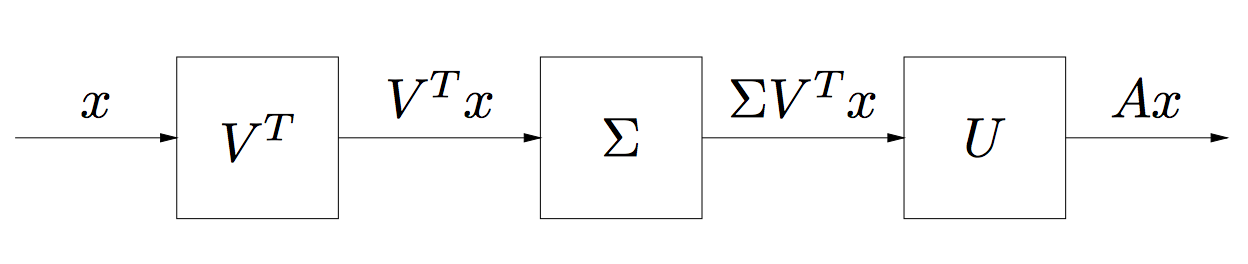
\includegraphics[width=17.33in]{images/math_svd001} 

}

\caption{SVD 그림.}\label{fig:unnamed-chunk-10}
\end{figure}

가 된다. 선형 사상(mapping) \(y=Ax\)는 다음과 같이 분해할 수 있다.

\begin{itemize}
\item
  \(x\)를 input direction들 \(v_{1}, \ldots , v_{n}\)을 따라 계수들을
  계산한다.
\item
  \(\sigma_{i}\)는 척도계수
\item
  이것들을 다시 output directions \(u_{1}, \ldots, u_{n}\)을 따라
  재구성한다.
\end{itemize}

대칭행렬 \(A\)에 대한 고유값 분해와 달라지는 점은 input direction들과
output direction들이 다르다는 것이다.

\begin{itemize}
\item
  \(v_{1}\)는 input direction으로 가장 민감하다.(most sensitive, highest
  gain)
\item
  \(u_{1}\)은 output direction으로 가장 민감하다.
\item
  \(Av_{1}=\sigma_{1}u_{1}\)이다.
\end{itemize}

\BeginKnitrBlock{example}[SVD의 기하학적 의미 예]
\protect\hypertarget{exm:unnamed-chunk-11}{}{\label{exm:unnamed-chunk-11}
\iffalse (SVD의 기하학적 의미 예) \fi{}
}\(A=\mathbb{R}^{2\times 2}\)이며 \(\Sigma=\text{diag}(1,0.5)\)인 경우를
생각해보자. 이 경우 \(x\)를 \(v_{1}\), \(v_{2}\)를 따라 풀면
\(v_{1}^{T}x=0.5, v_{2}^{T}x=0.6\) 즉 \(x=0.5v_{1} + 0.6v_{2}\)이며,
\(Ax=(v_{1}^{T}x)\sigma_{1}u_{1} + (v_{2}^{T}x)\sigma_{2}u_{2}= (0.5)(1)u_{1} + (0.6)(0.5)u_{2}\)
이다.
\EndKnitrBlock{example}

\begin{figure}

{\centering 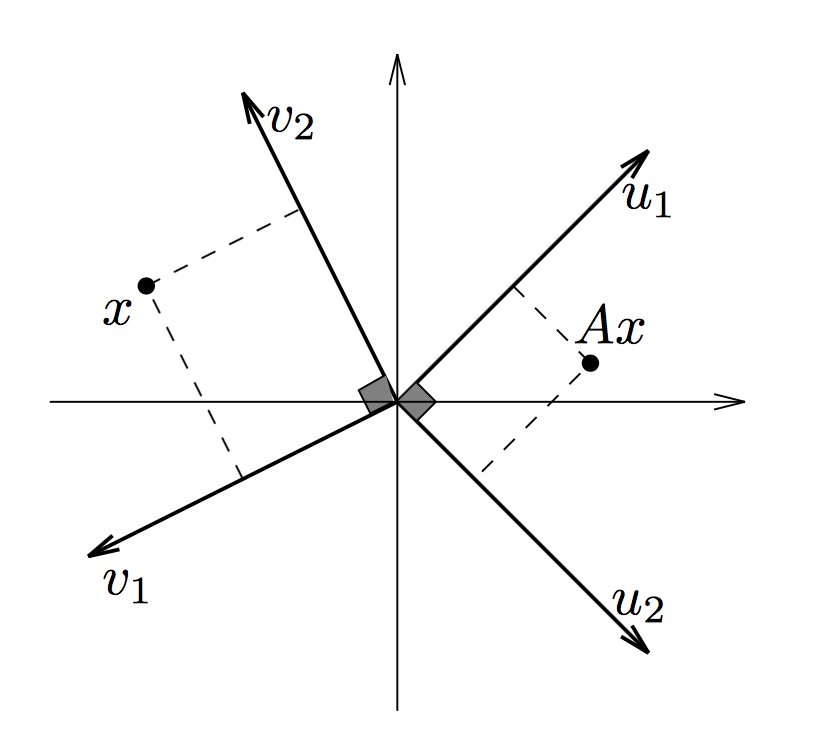
\includegraphics[width=11.5in]{images/math_svd002} 

}

\caption{SVD 예제 그림.}\label{fig:unnamed-chunk-12}
\end{figure}

\subsection{특이값 분해의 기하학적 의미}\label{---}

\href{https://en.wikipedia.org/wiki/Singular_value_decomposition}{위키피디아}를
참고하자.

\section{기저(basis)}\label{basis}

\subsection{Riesz basis}\label{riesz-basis}

In the Hilbert space \(L_{2}[0,1]\), an unconditional basis is called a
\textbf{Riesz basis} if it is ``almost normalized''. This means that
there exist real, positive, non-zero consts \(m\) and \(M\) so that
\[0 < m \leq \| \phi_{i}\|\leq M < \infty.\] A Riesz basis is
characterized by two Riesz constants \(A\) and \(B\), so that for all
\(f=\sum_{i}s_{i}\phi_{i}\in L_{2}[0,1]\),
\[A^{2}\| f \|^{2}\leq \sum_{i\in\mathbb{Z}}s_{i}^{2}\leq B^{2}\|f\|^{2}.\]

(Jensen의 Noise reduction and wavelet thresholding으로부터)

There exists \(\phi_{0}(x)\in\mathcal{V}_{1}\) such that
\(\{ \phi_{0}(x-k) | k\in\mathcal{Z} \}\) forms a Riesz basis of
\(\mathcal{V}_{1}\), i.e, there exists \(0< A \leq B <\infty\) such that
\[A \| c_{k}\|^{2} \leq \| \sum_{k}c_{k}\phi_{0}(x-k)\|^{2} \leq B \| c_{k} \|^{2}\]
for all \(\{c_{k}\}\in l^{2}\), where \(A\) and \(B\) do not depend on
the \(c_{k}\)

(동익이형 박사논문 47쪽)

\subsection{Radial basis function}\label{radial-basis-function}

Radial funtion이란 거리에만 의존하는 함수를 의미한다. 어떤 함수에 대한
근사 모델을 radial function의 선형조합으로 표현할 수 있다.

\begin{itemize}
\tightlist
\item
  Gaussian
\end{itemize}

\[\phi(r)=e^{-(\epsilon r)^{2}}\]

\begin{itemize}
\tightlist
\item
  Multiquadric
\end{itemize}

\[\phi(r)=\sqrt{1+(\epsilon r)^{2}}\]

\begin{itemize}
\tightlist
\item
  Inverse quadratic
\end{itemize}

\[\phi(r)=\frac{1}{1+(\epsilon r)^{2}}\]

\begin{itemize}
\tightlist
\item
  Inverse multiquadric
\end{itemize}

\[\phi(r)=\frac{1}{\sqrt{1+(\epsilon r)^{2}}}\]

\section{공간(space)}\label{space}

이 부분은 전체적으로 \citep{Shima2016}의 정의와 내용들을 따라간다.

\subsection{벡터 공간(vector space)}\label{-vector-space}

\subsubsection{완비 벡터 공간(complete vector
spaces)}\label{--complete-vector-spaces}

벡터 공간이 유한차원일 때, 공간의 완비성(completeness)은 같은 공간의
다른 larger orthonormal set에 포한되어 있지 않는 orthonormal set을
찾음으로써 증명할 수 있다. 예를 들면 3차원 공간에서는 linear
combination이 그 공간의 모든 벡터를 표현할 수 있는 three orthonormal
vector의 set을 찾기만 하면 되는 것이다. 그러나 우리가 무한 차원 공간을
고려할 때, 무한한 숫자의 orthonormal vector를 고려하는 것은 쉽지 않다.
사실 무한한 숫자의 vector의 linear combination은 때대로 같은 공간에
포함된 벡터를 표현하는 데 충분치 않을 수도 있다. 이러한 모호함을
해결하기 위해 무한 차원 공간에서 완비성을 생각하는 것이다.

\BeginKnitrBlock{definition}[벡터의 Cauchy sequence]
\protect\hypertarget{def:unnamed-chunk-13}{}{\label{def:unnamed-chunk-13}
\iffalse (벡터의 Cauchy sequence) \fi{} }벡터의 수열
\(\{ \mathbf{x}_{1},\mathbf{x}_{2},\ldots \}\)가 모든 \(\epsilon >0\)에
대해 적단한 근사 숫자 \(N\)이 존재해 모든 \(m,n > N\)에 대해
\(\| \mathbf{x}_{m} -\mathbf{x}_{n} \| < \epsilon\)을 만족한다면 이를
벡터의 \textbf{코시 수열(Cauchy sequence)}이라고 한다. 쉽게 얘기하자면
\(\mathbf{x}_{m}\)과 \(\mathbf{x}_{n}\)이 \(m,n \rightarrow \infty\)
함체 따라 가까어지는 수열을 코시 수열이라 부르는 것이다.
\EndKnitrBlock{definition}

\BeginKnitrBlock{definition}[코시 수열의 수렴]
\protect\hypertarget{def:unnamed-chunk-14}{}{\label{def:unnamed-chunk-14}
\iffalse (코시 수열의 수렴) \fi{} }벡터의 무한 수열
\(\{\mathbf{x}_{1},\mathbf{x}_{2}, \ldots \}\)가 있을 때, 만약
\(\mathbf{x}\)가 존재해
\(\| \mathbf{x}_{n} -\mathbf{x}\|\rightarrow 0\)을 만족한다면 이 수열이
수렴(convergent)한다고 한다.
\EndKnitrBlock{definition}

\subsection{위상공간(topological space)}\label{topological-space}

\subsection{분해 가능 공간(separable space)}\label{--separable-space}

Countable dense subset을 포함하는 위상공간(topological space)을
\textbf{분해 가능 공간(separable space)}이라고 한다.

\subsection{노름 공간(normed space)}\label{-normed-space}

\BeginKnitrBlock{definition}[노름 공간]
\protect\hypertarget{def:unnamed-chunk-15}{}{\label{def:unnamed-chunk-15}
\iffalse (노름 공간) \fi{} }원소들에 일종의 `길이' 또는 '크기'가 부여된
벡터 공간 \(V\)을 \textbf{노름 공간(normed space)}라고 한다.
\EndKnitrBlock{definition}

\subsection{바나흐 공간(Banach space)}\label{-banach-space}

\BeginKnitrBlock{definition}[힐버트 공간]
\protect\hypertarget{def:unnamed-chunk-16}{}{\label{def:unnamed-chunk-16}
\iffalse (힐버트 공간) \fi{} }Normed space가 complete일 경우 이를
\textbf{바나흐 공간(Banach space)}라고 부른다.
\EndKnitrBlock{definition}

유한차원에서 노름공간은 항상 완비(complete)이다. 그러나 무한차원에서
노름공간은 완비일 수도 있고, 아닐 수도 있다.

\BeginKnitrBlock{definition}[원-힐버트 공간]
\protect\hypertarget{def:unnamed-chunk-17}{}{\label{def:unnamed-chunk-17}
\iffalse (원-힐버트 공간) \fi{} }Inner product spaces들 중 완비가 아닌
공간들을 \textbf{원-힐버트 공간(pre-Hilbert space)}라고 부른다.
\EndKnitrBlock{definition}

\subsection{힐버트 공간(Hilbert space)}\label{-hilbert-space}

\BeginKnitrBlock{definition}[힐버트 공간]
\protect\hypertarget{def:unnamed-chunk-18}{}{\label{def:unnamed-chunk-18}
\iffalse (힐버트 공간) \fi{} }A complete normed space endowed with inner
product is called a \textbf{Hilbert space}
\EndKnitrBlock{definition}

다음 그림은 \citep{Shima2016}에 있는 그림으로 각 공간들 간의 사이의
관계를 이해하는 데 도움이 된다.

\begin{figure}

{\centering 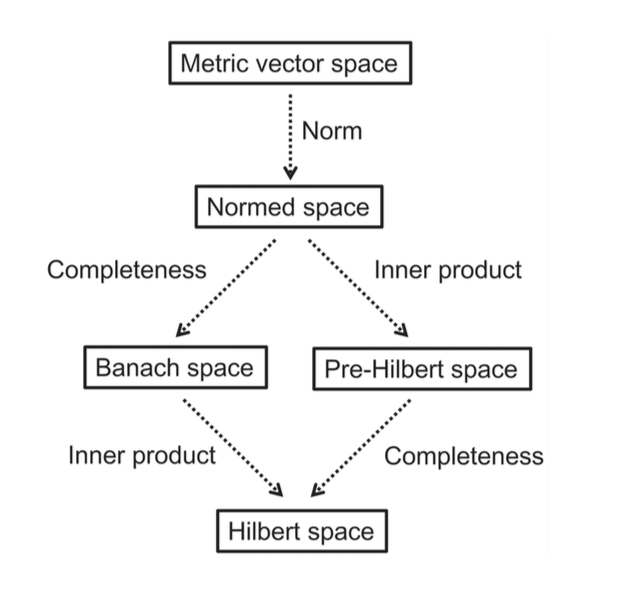
\includegraphics[width=8.58in]{images/math_Hilbertspacemap} 

}

\caption{Metric vector space로부터 힐버트 공간까지의 관계.}\label{fig:unnamed-chunk-19}
\end{figure}

힐버트 공간의 대표적인 예로, \(L^{p}\) 공간이 있다.

\[\| f\|_{p}=(\int_{S}|f|^{p}d\mu)^{1/p}<\infty\]

\subsection{Holder 공간(Holder space)}\label{holder-holder-space}

이 공간의 정의는 \citep{Wasserman2006}를 참고하였다. 어떤 정수 \(m\)과
\(\delta \in (0,1)\)에 대해 \(s=m+\delta\)을 정의하자. \textbf{Holder
공간(Holder space)}(정확하게는 H"\{o\}lder space)은 bounded m차
derivative를 갖는, 즉 모든 \(u,t\)에 대해
\(|f^{m}(u)-f^{m}(t)|\leq |u-t|^{\delta}\)인 bounded function들의
집합니다.

\subsection{Sobolev 공간(Sobolev space)}\label{sobolev-sobolev-space}

이 공간의 정의는 \citep{Wasserman2006}를 참고하였다. 이 책에서 Sobolev
공간의 정의는 smooth function들의 집합이라는 것이다. \(D^{j}f\)를
\(f\)의 \(j\)번째 weak derivative라고 하자. 먼저 weak
differentiability에 대해 알아보자. \(f\)가 모든 bounded interval에서
적분 가능하다고 하자. 만약 다음꽈 같은 함수 \(f'\)가 존재해 모든 bounded
interval에서 적분 가능하다면, 즉 모든 \(x\leq y\)에 대해
\[\int_{x}^{y}f'(s)ds=f(y)-f(x)\] 이라면 이를 \textbf{weakly
differentiable}이라 부른다.

\BeginKnitrBlock{definition}[Sobolev 공간]
\protect\hypertarget{def:unnamed-chunk-20}{}{\label{def:unnamed-chunk-20}
\iffalse (Sobolev 공간) \fi{} }\textbf{m차 Sobolev space}는 다음과 같다.
\[W(m)=\{ f \in L^{2}(0,1): D^{m}f \in L^{2}(0,1)\}\]

반지를 \(c\)를 갖는 \(m\)차 Sobolev space는 다음과 같다.
\[W(m,c)=\{ f \in W(m), \| D^{m}f \|^{2} \leq c^{2}\}\]

\textbf{주기를 갖는 Sobolev class (periodic Sobolev class)}는 다음과
같다.
\[\tilde{W}(m,c)=\{ f \in W(m,c): D^{j}f(0)=D^{j}f(1), j=0,\ldots, m-1 \}.\]
\EndKnitrBlock{definition}

\subsection{Besov 공간(Besov space)}\label{besov-besov-space}

이 공간의 정의 또한 \citep{Wasserman2006}의 9장을 참고하였다. Wavelet
threshold estimator는 Besov space에서 good optimality property를 갖는다.
다음과 같이 \(\Delta_{h}^{(r)}f(x)\)를 정의하자.
\[\Delta_{h}^{(r)}f(x)=\sum_{k=0}^{r}\binom{r}{k}(-1)^{k}f(x+kh).\]
그러면 \(\Delta_{h}^{(0)}f(x)=f(x)\)이고
\[\Delta_{h}^{(r)}f(x)=\Delta_{h}^{(r-1)}f(x+h)-\Delta_{h}^{(r-1)}f(x).\]
이다. 이제 \(w_{r,p}(f;t)\)를 다음과 같이 정의하자.
\[w_{r,p}(f;t)=\sup_{|h|\leq t}\|\Delta_{h}^{(r)}f\|_{p}.\] 이 때
\(\|g\|_{p}=\{ \int |g(x)|^{p}dx \}^{1/p}\)이다. \((p,g,\zeta)\)가
주어졌을 때, \(r\)이 존재해 \(r-1\leq \zeta \leq r\)을 만족한다면,
\textbf{Besov seminorm} \(|f|_{p,q}^{\zeta}\)는
\[|f|_{p,q}^{\zeta}=[\int_{0}^{\infty}(h^{-\zeta}w_{r,p}(f;h))^{q}\frac{dh}{h}]^{1/q}\]
로 정의된다. \(q=\infty\)일 때는 다음과 같이 정의한다.
\[|f|_{p,\infty}^{\zeta}=\sup_{0<h<1}\frac{w_{r,p}(f;h)}{h^{\zeta}}\]

\BeginKnitrBlock{definition}[Besov 공간]
\protect\hypertarget{def:unnamed-chunk-21}{}{\label{def:unnamed-chunk-21}
\iffalse (Besov 공간) \fi{} }\textbf{Besov 공간(Besov space)}
\(B_{p,q}^{\xi}(c)\)는 \([0,1]\)에서 \(\mathbb{R}\)로 가는 함수 \(f\)들
중 \(\int |f|^{p}<\infty\)이고 \(|f|_{p,q}^{\zeta}\leq c\)인 \(f\)들의
집합니다.
\EndKnitrBlock{definition}

Sobolev space \(W(m)\)은 Besov ball \(B_{2,2}^{m}\)에 대응된다.
Generalized Sobolev space \(W_{p}(m)\)은 \(m\)차 미분에서 \(L^{p}\)
노름을 사용하는 데 이것은 거의 Besov space와 비슷하다. 사실
\(B_{p,1}^{m} \subset W_{p}(m) \subset B_{p,\infty}^{m}\)이다.
H"\{o\}lder space는 \(B_{\infty,\infty}^{m+\delta}\)와 같다. \(T\)를
bounded variation을 갖는 함수들을 포함하는 집합이라고 할 때,
\(B_{1,1}^{1}\subset T \subset B_{1,\infty}^{1}\)을 만족한다. 즉 Besov
space는 넓은 범위희 함수 공간들을 포함한다.

\subsection{Skorohod 공간(Skorohod
space)}\label{skorohod-skorohod-space}

\(D[a,b]\)을 right continuous하고 left limit을 갖는 함수들
\(z:[a,b]\rightarrow \mathbb{R}\)의 집합을 \textbf{Skorohod
공간(Skorohod space)}이라고 한다. \citep{VanderVaart2000} 257쪽에
나와있다.

\subsubsection{웨이블릿 expansion의 계수들로 이해하는 Besov 공간(Besov
spaces in terms of the coefficients of the wavelet
expansion)}\label{-expansion---besov-besov-spaces-in-terms-of-the-coefficients-of-the-wavelet-expansion}

\subsection{Reproducing kernel Hilbert
space}\label{reproducing-kernel-hilbert-space}

\section{거리(distance)}\label{distance}

군집분석 방법에서는 관측값들의 거리를 이용해 군집을 나눌 때 사용된다.

\begin{itemize}
\item
  유클리드 거리(Euclidean distance):
  \(d(x,y)=(\sum_{i=1}^{p}(x_{i}-y_{i})^{2})^{1/2}\)
\item
  민콥스키 거리(Minkowski distance):
  \(d(x,y)=(\sum_{i=1}^{p}(x_{i}-y_{i})^{m})^{1/m}\)
\item
  맨하탄 거리(Manhattan distance):
  \(d(x,y)=\sum_{i=1}^{p}|x_{i}-y_{i}|\)
\item
  표준화 거리(standardized distance):
  \(d(x,y)=(\sum_{i=1}^{p}(x_{i}-y_{i})^{2}/s_{i}^{2})^{1/2}\), 여기서
  \(s_{i}\)는 \(i\)번째 변수에 대한 표준편차
\item
  마할라노비스 거리(Mahalanobis distance):
  \(d(x,y)=(x-y)^{T}\boldsymbol{\Sigma}^{-1}(x-y)\), 여기서 \(\Sigma\)는
  공분산행렬
\item
  체비셰프 거리(Chebychev distance):
  \(d(x,y)=\max_{i=1,\ldots ,p}|x_{i}-y_{i}|\)
\end{itemize}

다음 거리들은 유클리드 거리와 더불어 공간통계에서 많이 쓰이는 것들이다.

\begin{itemize}
\item
  chordal distance (현 거리? 잘 모르겠음)
\item
  geodesic distance
\end{itemize}

\chapter{기초 확률론}\label{basicprob}

이 장에서는 앞으로 다룰 내용을 이해하기 위해 필요한 기본적인 확률 개념을
정리하였다. 대학원 과정의 확률론을 다룬 유명한 책들로는
\citep{Durrett2010}, \citep{Billingsley2012} 그리고 \citep{Chung2001}이
있다. 그 밖에 본인이 추천하는 책들은 다음과 같다. \citep{Gut2012}는
최근에 나온 대학원 확률론 입문서 교재로써 비교적 내용이 자세하다.
\citep{Schilling2005}는 삽화가 많고 저자가 연습문제의 답을 웹에
올려놓았다. \citep{Shorack2006}과 \citep{Proschan2016}는 통계학자의
입장에서 필요한 확률론 지식을 비교적 쉽게 서술하였다. 여기서는 앞서
언급한 모든 책들을 참고할 것이다.

\section{표본공간과 사건(sample space and
events)}\label{-sample-space-and-events}

통계학은 무작위(random) 또는 확률적(stochastic) 실험(experiment), 즉
어떤 결과가 나올지 미리 확실히 예측할 수 없는 실험들에 초점을 맞춘다.

\BeginKnitrBlock{definition}[표본공간]
\protect\hypertarget{def:unnamed-chunk-22}{}{\label{def:unnamed-chunk-22}
\iffalse (표본공간) \fi{} }어떤 무작위 실험의 \textbf{표본공간(sample
space)} \(\Omega\)는 그 실험에서 나올 수 있는 모든 결과들의 집합이다.
\EndKnitrBlock{definition}

\BeginKnitrBlock{example}[동전 던지기 실험]
\protect\hypertarget{exm:unnamed-chunk-23}{}{\label{exm:unnamed-chunk-23}
\iffalse (동전 던지기 실험) \fi{} }동전을 두 번 던지는 실험에서
\(\Omega=\{ HH, HT, TH, TT \}\)이다. 이러한 표본공간을 \textbf{(유한)
이산 표본공간(finite discrete sample space)}이라고 한다.
\EndKnitrBlock{example}

\BeginKnitrBlock{example}[동전 계속 던지기 실험]
\protect\hypertarget{exm:unnamed-chunk-24}{}{\label{exm:unnamed-chunk-24}
\iffalse (동전 계속 던지기 실험) \fi{} }이번에는 동전의 뒷 면이
나올때까지 동전을 계속해서 던지는 실험에 대해 살펴보자. 그러면
\[\{ T, HT, HHT, HHHT, \ldots, \{ HHH\ldots\} \}\] 와 같은 결과들의
수얼을 얻을 수 있다. 이를 만약 동전을 던진 횟수로 정리한다면
\[\{ 1,2,3,\ldots, ,\infty\}\] 로 볼 수 있다. 이러한 표본공간을
\textbf{(무한) 이산 표본공간(infinite discrete sample space)}라고 한다.
\EndKnitrBlock{example}

\BeginKnitrBlock{example}[지하철 도착 시간]
\protect\hypertarget{exm:unnamed-chunk-25}{}{\label{exm:unnamed-chunk-25}
\iffalse (지하철 도착 시간) \fi{} }우리가 지하철을 기다리고 있다고
가정해보자. 지하철은 \(T\) 시간마다 한 번씩 도착한다. 그러면 우리가
기다리는 시간에 대한 표본공간은 \[[0,T]=\{t:0\leq y \leq T\}\] 이다.
이러한 표본 공간은 \textbf{연속 표본공간(continuous sample space)}라고
한다.
\EndKnitrBlock{example}

\BeginKnitrBlock{definition}[사건]
\protect\hypertarget{def:unnamed-chunk-26}{}{\label{def:unnamed-chunk-26}
\iffalse (사건) \fi{} }\textbf{사건(event)}란 표본공간 \(\Omega\)의
임의의 부분집합(subset)을 의미한다.
\EndKnitrBlock{definition}

\BeginKnitrBlock{example}[사건의 예]
\protect\hypertarget{exm:unnamed-chunk-27}{}{\label{exm:unnamed-chunk-27}
\iffalse (사건의 예) \fi{} }- 앞서 동전을 두 번 던지는 실험에서 앞면이
하나만 나올 사건을 \(A\)라고 하면 \(A=\{ HT, TH \}\)이다.

\begin{itemize}
\tightlist
\item
  앞서 동전을 두 번 던지는 실험에서 적어도 한 번 앞면이 나올 사건을
  \(B\)라고 하면 \(A=\{ HH, HT, TH \}\)이다.
\end{itemize}
\EndKnitrBlock{example}

\section{시그마-체(sigma-field)}\label{-sigma-field}

앞서 표본공간 \(\Omega\)의 임의의 부분집합인 사건을 생각했는데, 그러면
이 사건들의 집합 \(\mathcal{F}\)에 대해서도 생각해 볼 수 있을 것이다.
그리고 사건들의 집합이 가져야 할 바람직한 성질들을 잘 정의하기 위해
시그마-체라는 개념을 도입한다.

\BeginKnitrBlock{definition}[대수(체)]
\protect\hypertarget{def:unnamed-chunk-28}{}{\label{def:unnamed-chunk-28}
\iffalse (대수(체)) \fi{} }어떤 집합(set) \(\Omega\)의 non-empty
collection (즉 \(\Omega\)의 subset들의 모임)을 \(\mathcal{F}\)라고 하자.
그러면 \(\mathcal{F}\)가

\begin{enumerate}
\def\labelenumi{\arabic{enumi}.}
\item
  \(\Omega \in \mathcal{F}\) (또는 \(\emptyset \in \mathcal{F}\))
\item
  \(A \in \mathcal{F}\)이면 \(A^{C} \in \mathcal{F}\),
\item
  \(A, B \in \mathcal{F}\) 이면 \(A\cup B \in \mathcal{F}\)
\end{enumerate}

를 만족할 때 \(\mathcal{F}\)를 \textbf{대수(algebra)} 또는
\textbf{체(field)}라고 부른다.
\EndKnitrBlock{definition}

시그마-체는 앞선 대수의 정의에서 두 번째 조건이 조금 바뀐 것이다.

\BeginKnitrBlock{definition}[시그마-체]
\protect\hypertarget{def:unnamed-chunk-29}{}{\label{def:unnamed-chunk-29}
\iffalse (시그마-체) \fi{} }어떤 집합(set) \(\Omega\)의 non-empty
collection을 \(\mathcal{F}\)라고 할 때, \(\mathcal{F}\)가

\begin{enumerate}
\def\labelenumi{\arabic{enumi}.}
\item
  \(\Omega \in \mathcal{F}\) (또는 \(\emptyset \in \mathcal{F}\))
\item
  \(A \in \mathcal{F}\)이면 \(A^{C} \in \mathcal{F}\),
\item
  \(A_{1}, A_{2}, \ldots \in \mathcal{F}\) 이면
  \(\bigcup_{i=1}^{\infty}A_{i} \in \mathcal{F}\)
\end{enumerate}

를 만족할 때 \(\mathcal{F}\)를 \textbf{시그마-대수(sigma-algebra)} 또는
\textbf{시그마-체(sigma-field)}라고 부른다.
\EndKnitrBlock{definition}

다음은 체와 시그마-체에 대한 간단한 사실들이다.

\BeginKnitrBlock{corollary}[시그마-체에 대한 사실들]
\protect\hypertarget{cor:unnamed-chunk-30}{}{\label{cor:unnamed-chunk-30}
\iffalse (시그마-체에 대한 사실들) \fi{} }1. 모든 체는 finite union에
대해 닫혀있다. 또한 같은 논리를 적용해 finite intersection에 대해서도
닫혀있다.

\begin{enumerate}
\def\labelenumi{\arabic{enumi}.}
\setcounter{enumi}{1}
\item
  모든 시그마-체 \(\mathcal{F}\)는 countable intersection에 대해서도
  닫혀있다. 즉,
  \[A_{1}, A_{2}, \ldots  \in \mathcal{F} \text{ 이면 }  \bigcap_{i=1}^{\infty}A_{i} = (\bigcap_{i=1}^{\infty}A_{i}^{C})^{C} \in \mathcal{F}.\]
  물론 모든 \(A_{1}^{C}, A_{2}^{C},\ldots\) 또한
  \(A_{1}^{C}, A_{2}^{C}, \ldots \in \mathcal{F}\) 이다.
\item
  \(\mathcal{F}\)가 non-void일 경우에는 모든 체 또는 시그마-체가 \(A\)를
  포함하고 있으면 \(A^{C}\) 또한 포함하고 있기 때문에
  \(\Omega=A \cup A^{C}\)와 \(\emptyset=\Omega^{C}\) 또한
  \(\mathcal{F}\)에 포함되어 있다. 따라서 첫 번째 조건을 생략해도 된다.
\end{enumerate}
\EndKnitrBlock{corollary}

\BeginKnitrBlock{example}[시그마-체의 예]
\protect\hypertarget{exm:unnamed-chunk-31}{}{\label{exm:unnamed-chunk-31}
\iffalse (시그마-체의 예) \fi{} }- 어떤 집합 \(\Omega\)에 대해,
\(\{\emptyset, \Omega\}\)는 시그마-체가 된다. 이 시그마-체는
\(\Omega\)의 부분집합으로 만들 수 있는 가장 작은 시그마-체이다.

\begin{itemize}
\item
  \(\Omega\)의 멱집합(power set, 어떤 집합의 모든 부분집합을 모은 집합)
  또한 시그마-체이며 이는 \(\Omega\)의 부분집합으로 만들 수 있는 가장 큰
  시그마-체이다.
\item
  \(A\in\Omega\)일 때 collection \(\{\emptyset, A, A^{C}, \Omega\}\)
  또한 간단히 만들 수 있는 시그마-체의 예다.
\end{itemize}
\EndKnitrBlock{example}

\BeginKnitrBlock{example}[체이나 시그마-체가 아닌 예]
\protect\hypertarget{exm:unnamed-chunk-32}{}{\label{exm:unnamed-chunk-32}
\iffalse (체이나 시그마-체가 아닌 예) \fi{} }다음은 \(\mathcal{F}\)가
체이나 시그마-체가 아닌 예이다. \(\Omega=(0,1]\)이고, \(\mathcal{F}\)는
\(\emptyset\)과 모든
\[(a,b], \qquad{a,b\in\mathbb{Q}, a,b\in [0,1], a<b}\] 와 \((a,b]\)의
모든 finite union을 포함한다고 하자. 그리고 \([z]\)를 z와 가장 가까운
정수로 반올림해주는 연산자라고 하자. 그러면 정의에 의해
\(\mathcal{F}\)는 체가 된다. 그러나 \(A_{n}=(a_{n},1]\),
\(a_{n}=\frac{10^{n}}{[10^{n}\pi]}\)라고 하면
\[A_{n}\in\mathcal{F} \text{이나 } \cup_{n=1}^{\infty}A_{n}=(\pi,1]\notin \mathcal{F}\]
이다. 따라서 \(\mathcal{F}\)는 시그마-체가 아니다.
\EndKnitrBlock{example}

\BeginKnitrBlock{example}[표본공간이 셀 수 있는 집합이면 멱집합이 사건들의 집합]
\protect\hypertarget{exm:unnamed-chunk-33}{}{\label{exm:unnamed-chunk-33}
\iffalse (표본공간이 셀 수 있는 집합이면 멱집합이 사건들의 집합) \fi{}
}표본공간 \(\Omega\)가 셀 수 있는 집합, 예를 들면
\(\{0,1,2,\ldots, \}\)라고 가정하자. 그리고 이 때 사건들의 집합
\(\mathcal{F}\)가 모든 singleton \(\omega_{i}, i=1,2,\ldots\)들을
포함하는 시그마-체가 되길 원한다고 가정하자. 그러면 \(\Omega\)의 모든
부분집합 \(E\)는 \(\cup_{i=1}^{\infty}\omega_{i}\)로 만들 수 있다. 즉
singleton들의 countable union으로 만들 수 있다. 그리고 countable union에
대해 시그마-체가 닫혀있기 때문에, \(\mathcal{F}\)가 \(\Omega\)의 어떤
부분집합 \(E\)들을 모두 포함한다는 결론에 이른다. 즉, \textbf{표본공간이
셀 수 있는 집합이면, 우리는 항상 멱집합을 사건들의 집합으로 써야 한다.}
\EndKnitrBlock{example}

\section{생성기들(generators)}\label{generators}

시그마-체에 대해 좀 더 자세히 살펴보기 위해,
\textbf{생성기(generator)}에 대해 알아보자. 표본공간 \(\Omega\)의
subset들의 collection \(\mathcal{A}\)가 있다고 하자. 그러면 멱집합은
항상 시그마-체이기 때문에, \(\mathcal{A}\)를 포함하는 시그마-체가 적어도
한 개 이상 있을 것이다. \(\mathcal{F}^{*}\)를 \(\mathcal{A}\)를 포함하는
모든 시그마-체의 모임, 즉
\[\mathcal{F}^{*}=\{\sigma\text{-algebras } \supset \mathcal{A}\}\] 라고
하자. 여기서 \(\mathcal{A}\)를 포함하는 \textbf{가장 작은} 시그마-체를
생각해보자. 즉
\[\mathcal{F}=\sigma(\mathcal{A})=\bigcap_{\{\mathcal{F}` \text{ $\sigma$-algebra }|\mathcal{A}\subset\mathcal{F}` \}}\mathcal{F}`=\bigcap_{\mathcal{G}\in\mathcal{F}^{*}}\mathcal{G}\]
인 \(\mathcal{F}\)가 존재하고 이를 \(\mathcal{A}\)\textbf{로부터 생성된
시그마-체(sigma alegbra genearted by} \(\mathcal{A}\)\textbf{)}라고
부른다.

\BeginKnitrBlock{example}[생성기들]
\protect\hypertarget{exm:unnamed-chunk-34}{}{\label{exm:unnamed-chunk-34}
\iffalse (생성기들) \fi{} }- 만약 \(\mathcal{A}=A\), 즉
\(\mathcal{A}\)가 single set일 경우
\(\sigma(\mathcal{A})=\{ \emptyset, A, A^{C}, \Omega\}\)이다.

\begin{itemize}
\tightlist
\item
  만약 \(\mathcal{A}\)가 시그마-체일 경우,
  \(\sigma(\mathcal{A})=\mathcal{A}\)다.
\end{itemize}
\EndKnitrBlock{example}

\section{확률공간(probability space)}\label{probability-space}

\BeginKnitrBlock{definition}[가측공간]
\protect\hypertarget{def:unnamed-chunk-35}{}{\label{def:unnamed-chunk-35}
\iffalse (가측공간) \fi{} }표본공간 \(\Omega\)와 이와 연관된 시그마-체
\(\mathcal{A}\)를 묶어 \((\Omega, \mathcal{A})\)를
\textbf{가측공간(measurable space)}이라고 한다.
\EndKnitrBlock{definition}

\BeginKnitrBlock{definition}[확률측도]
\protect\hypertarget{def:unnamed-chunk-36}{}{\label{def:unnamed-chunk-36}
\iffalse (확률측도) \fi{} }가측공간 \((\Omega, \mathcal{A})\)가 주어졌을
때 \textbf{확률측도(probability measure)} \(P\)는
\(P:\mathcal{A}\rightarrow [0,1]\)인 함수로

\begin{enumerate}
\def\labelenumi{\arabic{enumi}.}
\item
  \(P(\emptyset)=0\) and \(P(\Omega)=1\)
\item
  어떤 \(A\in\mathcal{A}\)에 대해 \(P(A)\geq 0\)
\item
  \textbf{(가산가법성(countable additivity))}: \(\{A_{n}, n\geq 1\}\)이
  disjoint라고 하면
  \(P(\bigcup_{n=1}^{\infty}A_{n})=\sum_{n=1}^{\infty}P(A_{n}).\)
\end{enumerate}

을 만족한다. 그리고 \((\Omega, \mathcal{A}, P)\)를 묶어
\textbf{확률공간(probability space)}라고 한다.
\EndKnitrBlock{definition}

이 확률측도는 \(\mathcal{A}\)가 시그마-체일 때 뿐 아니라 그냥 체 일때도
위 세 가지를 만족하면 정의할 수 있다.

\section{보렐 시그마-체(Borel sigma field)}\label{--borel-sigma-field}

이제 \(\Omega\)가 비가산집합(uncountable set)일 때 시그마-체에 대해
살펴보자. 비가산집합의 대표적인 예로 \(\mathbb{R}\)이 있으니
\(\Omega=\mathbb{R}\)이라 놓고 전개하기로 한다. 앞서 얘기했듯이
시그마-체의 크기는 우리가 고려하고 싶은 모든 사건들과 그 사건들의
countable union, intersection을 적절히 잘 포함하는 정도여야 한다. 가장
쉽게 만들 수 있는 것은 \(\mathcal{F}\)가 모든 countable subset \(E\)를
포함하게끔 만드는 것이다. 그러나 이 시그마-체는 충분히 크지 않다. 예를
들어 \(\Omega=[0,1]\)일 경우, 앞서 말한 대로 \(\mathcal{F}\)를 만들면
\([0,0.5]\)같은 사건은 countable이나 co-countable이 아니므로
\(\mathcal{F}\)에 포함이 되지 않는 것이다.

즉 우리는 \(\Omega\)의 모든 interval들을 포함하는 시그마-체를 만들고
싶어한다.예를 들면, \(\Omega=[0,1]\)일 때
\[(a,b)\in\mathcal{F}, \qquad{(0\leq a < b \leq 1),}\]
\[P((a,b))=b-a, \qquad{(0\leq a < b \leq 1)}\] 이 되길 원하는 것이다.
가장 간단한 방법으로, 멱집합을 \(\mathcal{F}\)로 나용할 수 있다. 그러나
이 \(\mathcal{F}\)은 너무 크다. \(\mathcal{F}\)가 너무 클 경우,
확률측도가 잘 construct되지 않는 경우가 생길 수 있다고 한다.

\subsection{연속 표본공간에서 시그마-체로 멱집합을 쓰지 않는 이유(no
uniform probablity of power set on continous sample
space)}\label{-------no-uniform-probablity-of-power-set-on-continous-sample-space}

멱집합이 시그마-체로 적합하지 않은 이유로 (\([0,1], 2^{[0,1]}\))에서
균등확률이 존재하지 않음을 보일 것이다. \(P\)를
(\([0,1], 2^{[0,1]}\))에서 균등확률의 한 후보라고 놓자. 우리는 \(P\)가
\[P\{[a,b]\}=P\{(a,b)\}=P\{[a,b)\}=P\{(a,b]\}=b-a, \qquad{\text{for any }[a,b]\subseteq [0,1]}\]
을 만족하길 원한다. 또한 특별히
\[P\{a\}=0, \qquad{\text{for every }0\leq a \leq 1}\] 이다. 그리고
\(P\)는 확률의 공리(the axioms of probability) 중 하나인
가산가법성(countable additivity)을 만족시켜야 한다. 즉
\(0\leq a_{1}<b_{1}<\cdots <a_{n}<b_{n}<\cdots \leq 1\)이면 \(P\)는
\[P\{\bigcup_{i=1}^{\infty}[a_{i},b_{i}]\}=\sum_{i=1}^{\infty}P\{[a_{i},b_{i}]\}=\sum_{i=1}^{\infty}(b_{i}-a_{i})\]
를 만족해야 한다.

또한 \(P\)는 이동불변(shift invariant) 성질을 가져야 한다. 즉, 확률은
interval의 length에만 영향을 받아야 한다.
\[P\{[r,1/4 +r]\}=\frac{1}{4}, \qquad{\text{for every } 0 < r \leq 3/4.}\]
그런데 한 가지 문제가 생기는데 \(3/4 <r < 1\)이면 \([r,1/4+r]\)이
\([0,1]\)의 부분집합이 되지 않는다. 이를 해결하기 위해 ``wrapping
around''라는 방법을 이용한다. 만약 ``wrapping around''를 \(\oplus\)로
나타낸다면

\[
[0,1/4]\oplus r = 
\begin{cases}
[r, 1/4 + r] & \text{if $0 < r \leq 3/4$} \\
[0,1/4+r-1]\cup [r,1] & \text{if $3/4 < r < 1$}\\
\end{cases}
\] 로 정의하는 것이다. 그러면 \(A\subseteq [0,1]\)이라고 할 때 \(A\)를
\(r (0<r<1)\)만큼 이동하는 것을
\[A\oplus r = \{ a+r : a \in A, a+r \leq 1 \} \cup \{ a+r-1: a\in A, a+r > 1\}\]
로 정의할 수 있다.

\begin{figure}

{\centering 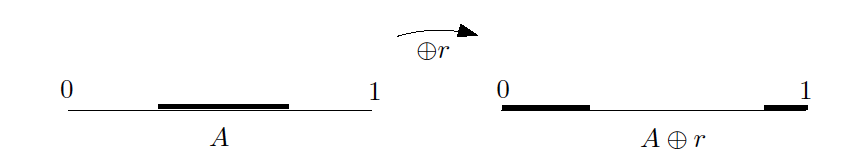
\includegraphics[width=12.06in]{images/basic_shift} 

}

\caption{Shift invariance.}\label{fig:unnamed-chunk-37}
\end{figure}

``wrapping around''를 이용해 \(A\)를 \(r\)만큼 이동해도 길이가 보존되기
때문에, 확률 또한
\[P\{ A \oplus r \}=P\{ A \}, \qquad{\text{for any } 0 < r < 1}\] 이 될
것이라 추론할 수 있다.

이제 모든 \(A \in 2^{[0,1]}\)에 대해 균등확률이 존재하지 않음을 보이기
위해 동치관계(equivalence relation)라는 것에 대해 정의할 것이다. \(x\)와
\(y\) (\(x,y \in [0,1]\))는 \(y-x\in\mathbb{Q}\)를 만족할 경우
동치관계라 정의하고 \(x \sim y\)로 표시한다. 예를 들면
\[\frac{1}{2} \sim \frac{1}{4}, \frac{1}{3} \sim \frac{1}{\pi}, \frac{1}{\pi}-\frac{1}{4} \sim \frac{1}{\pi}+\frac{1}{2} \]
인 것이다.

이 동치관계는 \([0,1]\)을 다음과 같이 분리(disjoint) 합집합들로 표현할
수 있다.
\[[0,1]=\mathbb{Q}_{1} \cup \{ \bigcup_{x\in [0,1] \backslash \mathbb{Q}_{1}} \{ (\mathbb{Q}+x)\cap [0,1] \} \}=\mathbb{Q}_{1} \cup \{ \bigcup_{x\in [0,1] \backslash \mathbb{Q}_{1}} \{ (\mathbb{Q}+x)\oplus x \} \}.\]

\begin{figure}

{\centering 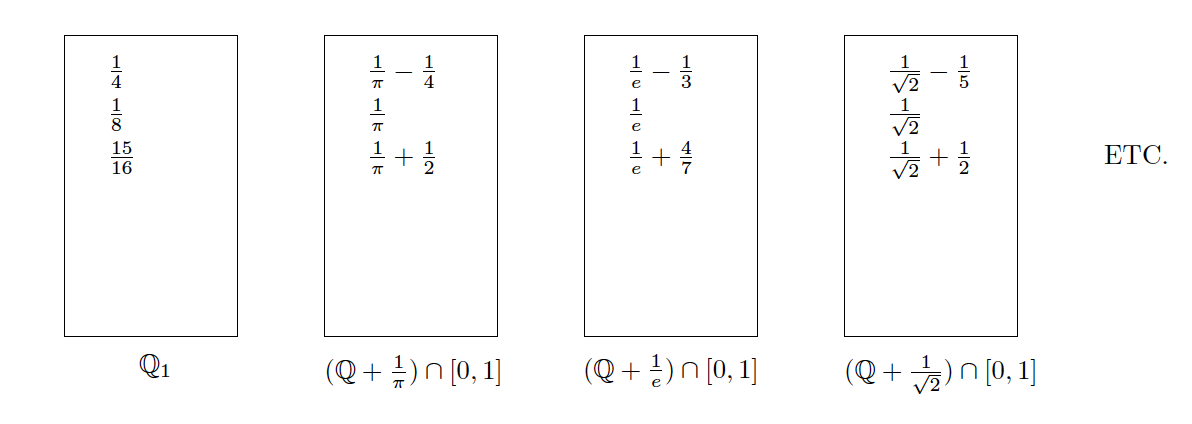
\includegraphics[width=16.56in]{images/basic_disjoint} 

}

\caption{Collection of disjoint unions on [0,1]}\label{fig:unnamed-chunk-38}
\end{figure}

\(H\)를 선택공리(the Axiom of Choice)에 의해 \([0,1]\)의 모든
동치관계에서 원소를 한 개씩 잘 뽑아서 만든 \([0,1]\)의 부분집합이라고
하자. 편의상 \(0\notin H\)라고 하자. 그러면 \((0,1]\)을
\[(0,1]=\bigcup_{r\in\mathbb{Q}_{1}, r\neq 1}\{ H \oplus r\} \qquad{\text{with }\{H\oplus r_{i}\} \cap \{H\oplus r_{j}=\emptyset \text{ for all } i\neq j\} } \]
로 표현할 수 있다. 그러면
\[1=P\{(0,1]\}=P\{ \bigcup_{r\in\mathbb{Q}_{1}, r\neq 1}\{ H \oplus r\} \}=\sum_{r\in \mathbb{Q}_{1},r\neq 1}P\{ H \oplus r\}=\sum_{r\in \mathbb{Q}_{1},r\neq 1}P\{ H\}\]
가 된다. 만약 우리가 \(p=P\{H\}\)로 확률을 부여하고자 한다면

\begin{enumerate}
\def\labelenumi{\arabic{enumi}.}
\item
  \(p=0\)일 때에는
  \(1=\sum_{r\in \mathbb{Q}_{1},r\neq 1}P\{ H\}=\sum_{r\in \mathbb{Q}_{1},r\neq 1} p \sum_{r\in \mathbb{Q}_{1},r\neq 1} 0 = 0\)
  이므로 모순이다.
\item
  마찬가지로 \(0<p\leq 1\)일 때에는
  \(\sum_{r\in \mathbb{Q}_{1},r\neq 1} p =\infty\)이므로 모순이다.
\end{enumerate}

즉 \(H\)는 사건이 아닌 셈이 되고 \(P\{ H \}\)가 존재하지 않는다. 이상의
결과를 다음 정리로 요약해본다.

\BeginKnitrBlock{theorem}[연속 표본공간에서 시그마-체로 멱집합을 쓰지 않는 이유]
\protect\hypertarget{thm:unnamed-chunk-39}{}{\label{thm:unnamed-chunk-39}
\iffalse (연속 표본공간에서 시그마-체로 멱집합을 쓰지 않는 이유) \fi{}
}셀 수 없는 표본공간 \([0,1]\)에서 시그마-체 \(2^{[0,1]}\)을 고려할 경우
\(P\{[a,b]\}=b-a, \text{ for all } 0\leq a \leq b \leq 1\)과
\(P\{ A \oplus r\}=P\{A\}, \text{ for all } A\subseteq [0,1] \text{ and } 0 < r < 1\)을
동시에 만족하는 \(P: 2^{[0,1]}\rightarrow [0,1]\)은 존재하지 않는다.
\EndKnitrBlock{theorem}

다시말하면, 모든 \(A\subseteq [0,1]\)에 대해 균등확률 \(P\{ A \}\)를
정의할 수 없다는 것이다.

\subsection{실수공간에서 보렐 시그마-체(Borel sigma-field on
R)}\label{---borel-sigma-field-on-r}

따라서, 모든 interval을 포함하는 시그마-체들 중 가장 \textbf{작은}
시그마-체 \(\mathcal{F}\)를 찾는 것이 이상적일 것이다. 즉 우리는
\(\sigma(\text{intervals})\)를 찾고자 하는 것이다.

여기서 잠시 \(\mathbb{R}\)에서의 \textbf{보렐 시그마-체(Borel
sigma-algebra)}에 대해 살펴보자. \(\mathbb{R}\)에서의 모든 열린
집합(open set)들의 모임을 \(\mathcal{O}\)라고 하자. 그러면
\(\mathcal{O}\)는 시그마-체가 아니다. (왜냐하면 \(A\in\mathcal{O}\)이면
\(A^{C}\)는 닫힌 집합이고 따라서 \(A^{C}\notin\mathcal{O}\)이다.)

\BeginKnitrBlock{definition}[보렐 시그마-체]
\protect\hypertarget{def:unnamed-chunk-40}{}{\label{def:unnamed-chunk-40}
\iffalse (보렐 시그마-체) \fi{} }\(\mathbb{R}\)에서의 \textbf{보렐
시그마-체(Borel sigma-field, Borel sigma-algebra)} \(\mathcal{B}\)는
\(\mathcal{B}=\sigma(\mathcal{O})\)로 정의한다.
\EndKnitrBlock{definition}

결론은 \(\mathbb{R}\)에서의 보렐 시그마-체를 interval을 포함하는
시그마-체로 만들 수 있다는 것이다. 그 전에 증명을 위해 한 가지 정리를
언급하겠다.

\BeginKnitrBlock{theorem}[열린 집합과 열린 구간들]
\protect\hypertarget{thm:unnamed-chunk-41}{}{\label{thm:unnamed-chunk-41}
\iffalse (열린 집합과 열린 구간들) \fi{} }\(E \subseteq \mathbb{R}\)이
열린 집합이라고 하자. 그러면 기껏해야 셀 수 있는 정도로만 많은(at most
countably many) 열린 구간들(open intervals) \(I_{j}, j=1,2,\ldots,\)가
존재해 다음을 만족한다. \[E=\bigcup_{j=1}^{\infty}I_{j}.\]
\EndKnitrBlock{theorem}

\BeginKnitrBlock{proof}
\iffalse{} {Proof. } \fi{}이 정리의 증명은
\(E=\bigcup_{j=1}^{\infty}I_{j}\)를 만족하는 \(I_{j}\)들이 있음을 보이고
이것이 (1) at most countably many (2) disjoint (3) open (4) intervals
임을 보이면 된다. 증명 방법은 동치 관계를 이용하는 것이다.
\(a, b \in E, (a < b)\)일 때 열린구간 \((a,b)\subseteq E\)이면
\(a \sim b\)로 놓는다. 그러면 \(E\)의 disjoint union of classes는
equivalence relationship partitions \(E\)가 된다. 아직 이것들이
countably many한지 모르므로 이들을
\(I_{j}, j\in J, J \text{ is an arbitrary index set}\)이라고 높자.
임의의 \(a_{j}<b_{j}\in I_{j}\)에 대해 \(a_{j} \sim b_{j}\)이고
\((a_{j}, b_{j}) \in I_{j}\)이므로 \(I_{j}\)는 interval이다. 또
\(x\in I_{j}\)를 임의로 뽑았을 때 \(x\in E\)이고 \(E\)가 open이므로,
\((x-\epsilon, x+\epsilon)\subseteq E\)를 만족하는 \(\epsilon >0\)이
모든 \(x\)에 대해 존재함을 알 수 있고 ahems
\(a\in (x-\epsilon, x+\epsilon)\)에 대해 \(a \sim x\)이므로 \(x\)의
\(\epsilon\)-근방은 \(I_{j}\)에 포함됨을 알 수 있어 \(I_{j}\)는
open이다. 마지막으로 모든 \(I_{j}\)는 적어도 하나의 유리수를 포함하고
있어 이를 통해 \(I_{j}\)의 갯수는 countably many임을 알 수 있다.
\EndKnitrBlock{proof}

\BeginKnitrBlock{theorem}[실수 구간에서의 보렐 시그마-체의 생성]
\protect\hypertarget{thm:unnamed-chunk-43}{}{\label{thm:unnamed-chunk-43}
\iffalse (실수 구간에서의 보렐 시그마-체의 생성) \fi{}
}\(\mathbb{R}\)에서의 보렐 시그마-체(Borel sigma-field, Borel
sigma-algebra) \(\mathcal{B}\)는 \((-\infty, a], a\in\mathbb{Q}\)로
생성할 수 있다.
\EndKnitrBlock{theorem}

\BeginKnitrBlock{proof}
\iffalse{} {Proof. } \fi{}\(\mathcal{O}_{0}\)을 \(\mathbb{R}\)에서의
모든 열린 구간(open interval)들의 collection이라고 하자. 앞선 정리에
의해 \(\mathbb{R}\)에서의 모든 열린 집합은 기껏해야 셀 수 있을 정도의
열린 구간의 합집합으로 나타낼 수 있으므로
\(\sigma(\mathcal{O}_{0})=\mathcal{B}\)가 된다. \(\mathcal{D}\)를
\((-\infty, a], a\in \mathbb{Q}\)인 구간들의 collection이라고 하자.
그리고 구간 \((a,b)\)를
\((a,b)\in \mathcal{O}_{0}, a,b \in \mathbb{Q}, a<b\)와 같이 정의하자.
여기서 \[a_{n}=a+\frac{1}{n} \text{ and } b_{n}=b-\frac{1}{n}\] 으로
놓으면
\[(a,b)=\bigcup_{n=1}^{\infty}(a_{n},b_{n}]=\bigcup_{n=1}^{\infty}\{ (-\infty, b_{n}] \cap (-\infty, a_{n}]^{c}\}\]
이다. 이것은 \((a,b)\in \sigma (\mathcal{D})\)임을 의미한다. 즉
\(\mathcal{O}_{0}\subseteq \sigma(\mathcal{D})\)이고
\(\sigma(\mathcal{O}_{0})\subseteq \sigma(\mathcal{D})\)이다. 그러나
\(\mathcal{D}\)의 모든 원소는 닫힌 집합이고 이는
\(\sigma(\mathcal{D})\subseteq \mathcal{B}\)를 의미한다. 따라서
\[\mathcal{B} = \sigma(\mathcal{O}_{0})\subseteq \sigma(\mathcal{D})\subseteq \mathcal{B}\]
이므로 \(\sigma(\mathcal{D})=\mathcal{B}\)이다.
\EndKnitrBlock{proof}

이제 \([0,1]\subset \mathbb{R}\)에서의 보렐 시그마-체
\(\mathcal{B}_{1}\)을 생각해보자. 이는 \(\mathcal{B}\)와 마찬가지로
\([0,1]\)의 열린 부분집합들의 collection으로부터 생성된 시그마-체라고
생각할 수 있다. 한 가지 주의해야 할 점은 \(\mathcal{B}_{1}\)은
\(\mathcal{B}\)의 부분 시그마-체는 아니라는 것이다. 시그마-체에서 포함
관계를 얘기하려면 두 시그마-체의 표본공간이 같아야 한다.

\subsection{실수공간에서 확률측도의 구성(construction of a probability
measure on R)}\label{--construction-of-a-probability-measure-on-r}

이제 앞서 언급한 보렐 시그마-체 \(\mathcal{B}_{1}\)을 이용해 균등한
확률을 만드는 작업을 진행할 것이다. 전략은 먼저
\textbf{단조족정리(monotone class theorem)}을 증명한 후 그것의
따름정리를 이용해 모든 \(0\leq a \leq b \leq 1\)에서 균등확률
\(P\{[a,b]\}=b-a\)를 정의한 후 이것을 \([0,1]\)의 보렐집합으로 확장하는
것이다.

\(\mathcal{F}_{0}\)를 표본공간 \(\Omega\)에서의 부분집합들의
collection이라고 하자. 그러면 \(\mathcal{F}_{0}\)에서 확률측도
\(P:\mathcal{F}_{0} \rightarrow [0,1]\)을 정의한다. 그리고
\(\mathcal{F}=\sigma(\mathcal{F}_{0})\)의 확률측도
\(Q:\mathcal{F} \rightarrow [0,1]\)가
\(Q\{A\}=P\{A\} \forall A\in \mathcal{F}_{0}\)인 성질을 가진체로
정의된다는 것을 보인다. 마지막으로 이 \(Q\)가 유일함을 보일 것이다.

그 전에 몇 가지 개념들에 대해 정의하겠다.

\BeginKnitrBlock{definition}[유한한 교집합에 대해 닫혀있다]
\protect\hypertarget{def:unnamed-chunk-45}{}{\label{def:unnamed-chunk-45}
\iffalse (유한한 교집합에 대해 닫혀있다) \fi{} }표본공간 \(\Omega\)의
부분집합들의 class \(\mathcal{C}\)가
\[\bigcap_{i=1}^{n}A_{i}\in\mathcal{C}\qquad{\text{for every }n\infty \text{ and } A_{1},\ldots ,A_{n}\in\mathcal{C}}\]
를 만족하면 \textbf{유한한 교집합에 대해 닫혀있다(closed under finite
intersection)}라고 한다.
\EndKnitrBlock{definition}

\BeginKnitrBlock{definition}[증가하는 극한에 대해 닫혀있다]
\protect\hypertarget{def:unnamed-chunk-46}{}{\label{def:unnamed-chunk-46}
\iffalse (증가하는 극한에 대해 닫혀있다) \fi{} }표본공간 \(\Omega\)의
부분집합들의 class \(\mathcal{C}\)가
\[\bigcup_{i=1}^{\infty}A_{i}\in\mathcal{C}\qquad{\text{for every collection } A_{1}, A_{2},\ldots \in \mathcal{C} \text{ with } A_{1}\subseteq A_{2}\subseteq \ldots}\]
를 만족하면 \textbf{증가하는 극한에 대해 닫혀있다(closed under
increasing limits)}라고 한다.
\EndKnitrBlock{definition}

\begin{figure}

{\centering 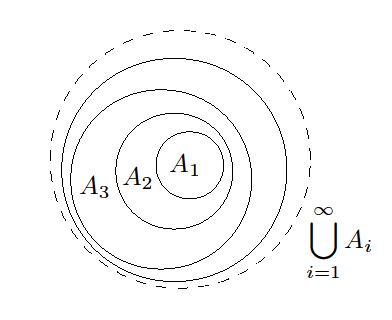
\includegraphics[width=5.44in]{images/basic_cuil} 

}

\caption{Closed under increasing limits.}\label{fig:unnamed-chunk-47}
\end{figure}

\BeginKnitrBlock{definition}[유한한 차에 대해 닫혀있다]
\protect\hypertarget{def:unnamed-chunk-48}{}{\label{def:unnamed-chunk-48}
\iffalse (유한한 차에 대해 닫혀있다) \fi{} }표본공간 \(\Omega\)의
부분집합들의 class \(\mathcal{C}\)가 모든
\(A,B\in\mathcal{C}, A\subseteq B\)에 대해
\(B\backslash A \in \mathcal{C}\)를 만족하면 \textbf{유한한 차에 대해
닫혀있다(closed under finite differences)}라고 한다.
\EndKnitrBlock{definition}

\begin{figure}

{\centering 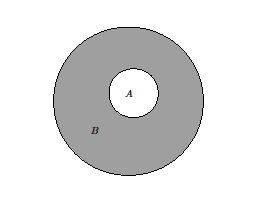
\includegraphics[width=3.67in]{images/basic_cufd} 

}

\caption{Closed under finite differences.}\label{fig:unnamed-chunk-49}
\end{figure}

다음은 단조족에 대한 정의다.

\BeginKnitrBlock{definition}[단조족]
\protect\hypertarget{def:unnamed-chunk-50}{}{\label{def:unnamed-chunk-50}
\iffalse (단조족) \fi{} }표본공간 \(\Omega\)의 부분집합들의 class
\(\mathcal{C}\)가 closed under countable increasing set이거나 closed
under countable decreasing set이면, 즉
\(E_{1},E_{2},\ldots \in \mathcal{C}\)일 때
\[E_{i}\uparrow E \text{ or } E_{i}\downarrow E \Longrightarrow E \in \mathcal{C}\]
이면 \(\mathcal{C}\)를 \textbf{단조족(monotone class)}이라고 한다.
\EndKnitrBlock{definition}

이에 대한 증명은 \citep{Durrett2010}의 Appendix 부분을 참고하자.

\section{측도(measure)}\label{measure}

\textbf{측도(measure)}란 수학에서, \textbf{양(quantity)}이라 개념을
반영하기 위해 만들어진 장치다. \(X\)를 어떤 집합이라고 하고, 이것의
부분집합 \(U \subset X\)가 있을 때,

\subsection{Lebesgue 측도(Lebesgue
measure)}\label{lebesgue-lebesgue-measure}

\subsection{확률측도(probability measure)}\label{probability-measure}

\section{라돈-니코딤 정리(Radon-Nykodim
theorem)}\label{--radon-nykodim-theorem}

\chapter{확률변수}\label{rv}

\BeginKnitrBlock{definition}[가측]
\protect\hypertarget{def:unnamed-chunk-51}{}{\label{def:unnamed-chunk-51}
\iffalse (가측) \fi{} }\((\Omega_{1}, \mathcal{F}_{1})\),
\((\Omega_{2}, \mathcal{F}_{2})\)가 두 가측공간(measurable)이라고 할 때,
함수 \(X:\Omega_{1} \rightarrow \Omega_{2}\)가 임의의 집합
\(E\in \mathcal{F}_{2}\)에 대해 집합 \(X^{-1}(E)\)이
\[X^{-1}(E)=\{ \omega \in \Omega_{1}: X(\omega) \in E\} \mathcal{F}_{1}\]
(또는 위 조건을 \(X^{-1}(\mathcal{F}_{2})\in \mathcal{F}_{1})\)) 일 때
\(X\)가 \textbf{가측(measurable)}이라고 한다. (또는
\(\mathcal{F}_{1}\)-가측 이라고도 부른다.)
\EndKnitrBlock{definition}

\BeginKnitrBlock{definition}[확률변수]
\protect\hypertarget{def:unnamed-chunk-52}{}{\label{def:unnamed-chunk-52}
\iffalse (확률변수) \fi{} }\((\Omega, \mathcal{F}, P)\)가
확률공간(probability space)이라고 하자. 그러면 어떤 실변수 함수
\[X:\Omega \rightarrow \mathbb{R}\] 가 \((\Omega, \mathcal{F})\)에서
\((\mathbb{R}, \mathcal{B})\)로 가는 가측함수(measurable function)일
때(여기서 \(\mathcal{B}\)는 \(\mathbb{R}\)에서의 보렐 시그마-체) 이
\(X\)를 \textbf{확률변수(random variable)}라고 부른다.
\EndKnitrBlock{definition}

(확률변수에 대한 설명 보충 필요)

\section{보렐-칸텔리 따름정리}\label{--}

\BeginKnitrBlock{lemma}[보렐-칸텔리 따름정리]
\protect\hypertarget{lem:unnamed-chunk-53}{}{\label{lem:unnamed-chunk-53}
\iffalse (보렐-칸텔리 따름정리) \fi{} }\textbf{(Borel-Cantelli lemma)}
만약 \(\sum_{n=1}^{\infty}P(A_{n}) < \infty\)라면 \[P(A_{n} i.o.)=0\]
이다.
\EndKnitrBlock{lemma}

\BeginKnitrBlock{lemma}[제 2 보렐-칸텔리 따름정리]
\protect\hypertarget{lem:unnamed-chunk-54}{}{\label{lem:unnamed-chunk-54}
\iffalse (제 2 보렐-칸텔리 따름정리) \fi{} }\textbf{(Second
Borel-Cantelli lemma)} 만약 사건 \(A_{n}\)들이 독립이라면
\(\sum P(A_{n})=\infty\)는 \(P(A_{n} i.o.)=1\)임을 내포한다.
\EndKnitrBlock{lemma}

\chapter{확률변수의 수렴}\label{convergencerv}

\citep{Proschan2016}의 내용을 따라간다.

\section{거의 확실한 수렴(Almost sure
convergence)}\label{--almost-sure-convergence}

\(X_{1}, X_{2},\ldots\)가 확률공간 \((\Omega, \mathcal{F}, P)\)에서의
확률변수의 수열이라고 하자. 고정된 \(\omega\)에 대해
\(X_{n}(\omega)=x_{n}, n=1,2,\ldots\)은 숫자의 수열이라고 하자. 각
\(\omega\)에 대해 \(X_{n}(\omega)\)가 수렴할 수 있지만 극한
\(X(\omega)\)는 \(\omega\)에 따라 다를 수 있다. 예를 들면,
\((\Omega, \mathcal{F}, P)=([0,1],\mathcal{B}_{[0,1]},\mu_{L})\) 이고

\begin{equation}
X_{n}(\omega)=\omega^{n}
\label{eq:almostsureex01}
\end{equation}

이다. 그러면 \(n\rightarrow \infty\)일 때
\(X_{n}(\omega) \rightarrow I(\omega=1)\)이다. 그런데 어떤 \(\omega\)에
대해서는 \(X_{n}(\omega)\)는 극한이 없거나 무한대의 극한을 갖을 수 있다.
예를 들면 앞선 식 \eqref{eq:almostsureex01}을 다음과 같이 바꾸는 것이다.

\begin{equation}
X_{n}(\omega)=(-\omega)^{n}
\label{eq:almostsureex02}
\end{equation}

그러면 \(\omega < 1\)일 때 \(n\rightarrow 0\)이나 \(\omega=1\)일 때는
극한이 존재하지 않는다.

식 \eqref{eq:almostsureex01}과 \eqref{eq:almostsureex02}에서의 행동이
다르다고 하더라도 \(\{\omega=1\}\)이 확률 0을 갖는다면 다른 행동을
무시할 수 있을 것이다. 이것을 확장시키면 확률 0인 집합들을 무시하는
것으로 이해할 수 있고, \textbf{거의 확실한 수렴(Almost sure
convergence)}의 정의를 이끈다.

\section{확률수렴(Convergence in
probability)}\label{convergence-in-probability}

\section{Lp 수렴(Convergence in Lp)}\label{lp-convergence-in-lp}

\section{분포수렴(Convergence in
distribution)}\label{convergence-in-distribution}

\textbf{분포수렴(Convergence in distribution)}은 분포함수의 관계를
다룬다는 것에서 확률변수들의 관계를 고려하는 앞 수렴들과는 다른 타입의
수렴이라고 할 수 있다. \(X_{n}\)의 분포함수 \(F_{n}(x)\)가 \(X\)의
분포함수 \(F(x)\)로 수렴할 때 우리는 \(X_{n}\)이 \(X\)에 대해 분포적으로
가까워진다고 말한다. 가장 단순한 예로 \(X_{n}=1+\frac{1}{n}\)이고
\(X\)는 1인 경우를 생각해 볼 수 있다. 이 때 \(X_{n}\)의 분포함수
\(F_{n}(x)\)는 다음과 같은 분포함수 \(F(x)\)로 가까워지는 것처럼 보인다.

\begin{equation}
F(x)=
\begin{cases}
0 & \text{if } x < 1 \\
1 & \text{if } x \geq 1 
\end{cases}
\label{eq:distnconvex01}
\end{equation}

그러나 \(F_{n}(x)=P(X_{n}\leq x)\)는

\begin{equation}
F_{n}(x)=
\begin{cases}
0 & \text{if } x < 1 + \frac{1}{n} \\
1 & \text{if } x \geq 1 \frac{1}{n}
\end{cases}
\label{eq:distnconvex02}
\end{equation}

이며 이는

\begin{equation}
\begin{cases}
0 & \text{if } x \leq 1 \\
1 & \text{if } x > 1
\end{cases}
\end{equation}

로 수렴한다. 식 \eqref{eq:distnconvex01}과 식 \eqref{eq:distnconvex02}의
분포함수는 \(x=1\)에서 일치하지 않는다. 따라서, \(F_{n}(x)\)가 모든
\(x\)에서 \(F(x)\)로 수렴하는 것은 너무 강한 조건으로 보인다. 분포수렴을
정의할 때에는 앞선 예의 \(x=1\)처럼 불연속인 점들을 제외한 연속인 점들
\(x\)에서 \(F_{n}(x) \rightarrow F(x)\)가 되는 것으로 정의한다.

\section{수렴 사이들의 관계(Connections between modes of
convergence)}\label{--connections-between-modes-of-convergence}

\begin{figure}

{\centering 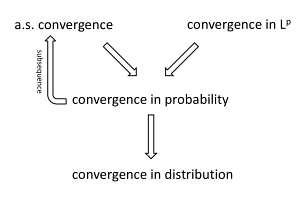
\includegraphics[width=4.28in]{images/basic_convergenceconnection} 

}

\caption{Connections between modes of convergences.}\label{fig:unnamed-chunk-55}
\end{figure}

\section{Convergence of moments: 일양적분가능성(uniform
integrability)}\label{convergence-of-moments-uniform-integrability}

\(X_{n}\)이 점근적으로 \(\mathcal{N}(\mu_{n}, \sigma_{n}^{2})\)에
수렴한다는 문장을 생각해보자. 즉 이 얘기는
\((X_{n}-\mu_{n})/\sigma_{n} \stackrel{D}{\rightarrow} \mathcal{N}(0,1)\)이라는
말이다. 그러나 이것이 \(E(X_{n})=\mu_{n}\)이고
\(\text{var}(X_{n})=\sigma_{n}^{2}\)임을 의미하지는 않는다. 일반적으로
\(X_{n} \stackrel{D}{\rightarrow} X\)는
\(E(X_{n}) \rightarrow E(X)\)임을 의미하지 않는다.

\BeginKnitrBlock{example}[추정량은 무한대의 평균을 갖으나 확률변수의 극한은 유한한 평균을 갖는 예]
\protect\hypertarget{exm:unnamed-chunk-56}{}{\label{exm:unnamed-chunk-56}
\iffalse (추정량은 무한대의 평균을 갖으나 확률변수의 극한은 유한한
평균을 갖는 예) \fi{} }\(\hat{p}_{n}\)이 iid 베르누이 확률변수
\(X_{1}, \ldots, X_{n}\)로부터 나온 표본비(sample proportion)라고 하자.
그러면 CLT에 의해 \(\hat{p}_{n}\)은 점근적으로 평균 \(p=E(X_{1})\)이고
분산 \(p(1-p)/n\)인 정규분포를 따른다. 델타 방법(delta method)에 의해
\(\text{ln}(\hat{p})\)는 점근적으로 평균 \(\ln(p)\), 분산
\((1-p)/(np)\)인 정규분포를 따름을 안다. 그러면
\[Z_{n} = \frac{\text{ln}(\hat{p}_{n})-\text{ln}(p)}{\sqrt{(1-p)/(np)}} \stackrel{D}{\rightarrow} Z \sim \mathcal{N}(0,1)\]
임을 안다. 그러나 모든 \(n\)에 대해
\(E\{\text{ln}(\hat{p}_{n}) \}=-\infty\)인데, 이는 \(\hat{p}_{n}\)은 0이
될 확률이 양수이기 때문이다. 그러므로 \(E(Z_{n})=-\infty\)이나,
\(E(Z)=0\)이다.
\EndKnitrBlock{example}

(Skrohod 정리를 이용한 추가적 설명 필요, Essential of Probability Theory
for Statisticians 193-194쪽)

\BeginKnitrBlock{definition}[일양적분가능]
\protect\hypertarget{def:unnamed-chunk-57}{}{\label{def:unnamed-chunk-57}
\iffalse (일양적분가능) \fi{} }만약 각 \(\epsilon >0\)에 대해
\[E\{ |X_{n}| I(|X_{n}|>A)\}<\epsilon \forall n\] 을 만족하는 \(A\)가
존재한다면 이 확률변수의 수열 \(X_{n}\)을 \textbf{일양적분가능(uniformly
integrable, UI)}이라고 부른다. 또는
\[\lim_{A\rightarrow\infty}\sup_{n}E\{ |X_{n}| I(|X_{n}|>A)\}=0\] 을
만족하는 것으로 정의하기도 한다.
\EndKnitrBlock{definition}

그렇다면 일양적분가능이 말하고자 하는 것은 무엇인가?
\(|X_{n}| I(|X_{n}|>A)\)항부터 살펴보자. 이것은 \(A\)보다 작은
\(|X_{n}|\) 값은 0이 되도록 조절하는 것이다. 다음 그림을 참고하자.

\begin{figure}

{\centering 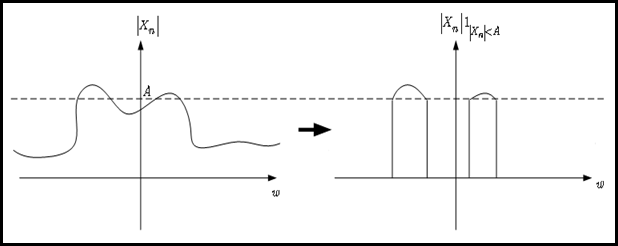
\includegraphics[width=8.58in]{images/basic_UI01} 

}

\caption{Case when function values bigger than A exist.}\label{fig:unnamed-chunk-58}
\end{figure}

다음은 \(E\{|X_{n}| I(|X_{n}|>A)\}\)에 초점을 맞춘다. 이것은 그림
\ref{fig:theoryUI01}의 그래프 아래 면적에 해당하는 것이다(물론
\(\omega \in [0,M]\)에서 균등한 확률 측도 \(dP(\omega)=\frac{1}{M}\)을
줬을 때의 이야기다). 이때 상한(\(\sup_{n}\))의 쓰임은 \(A\)가 고정되었을
때 가장 큰 면적을 반환하는 \(n\)을 찾는 것이다. 마지막으로 극한을
취함으로써(\(lim_{A\rightarrow\infty}\sup_{n}E\{ |X_{n}| I(|X_{n}|>A)\}\))
\(A\)가 점점 커졌을 때 상한이 어떻게 변하는지 관찰할 수 있다.

\begin{figure}

{\centering 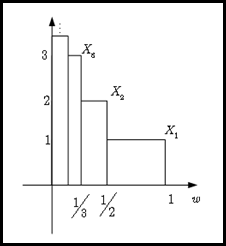
\includegraphics[width=3.14in]{images/basic_UI02} 

}

\caption{An example of sequence of random variables that is not uniformly integrable.}\label{fig:unnamed-chunk-59}
\end{figure}

위 확률변수의 수열은 일양적분가능하지 않다. \(A\)가 커짐에 따라 항상
\(E\{|X_{n}| I(|X_{n}|>A)\}=1\)을 만족하는 \(n\)이 존재한다. 즉
\(|X_{n}| I(|X_{n}|>A)=|X_{n}|\)인 \(n\)이 항상 존재하는 것이다. 따라서
\[\sup_{n}E\{ |X_{n}| I(|X_{n}|>A)\}=\sup_{n}E\{ |X_{n}|\}=\sup_{n}1=1.\]
이다.

\begin{figure}

{\centering 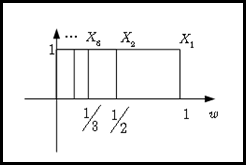
\includegraphics[width=3.42in]{images/basic_UI03} 

}

\caption{An example of sequence of random variables that is uniformly integrable.}\label{fig:unnamed-chunk-60}
\end{figure}

위 예들로부터 얻을 수 있는 직관적 사실들은 다음과 같다. 만약 \(X_{n}\)의
평균 면적이 \(n\)이 커짐에 따라 무한대로 발산하면 그 확률변수의 수열은
항상 일양적분가능하지 않을 것이다. 한편

\begin{itemize}
\item
  모든 유한한 수열을 항상 일양적분가능하다(왜냐하면 모든 고정된 \(n\)에
  대해 \(P(X_{n}>A)\)는 \(A\)가 커짐에 따라 감소한다).
\item
  모든 유계(bounded)인 확률변수의 수열(반대로 유계가 아닌 경우를
  생각해보면 \(n\)이 커짐에 따라 \(X_{n}\)은 어떤 확률로 점점 큰 값을
  갖게 될 것이다)일양적분가능하다. 그러나 그 역은 성립하지 않는다.
\end{itemize}

마지막으로 유계가 아니나 일양적분가능한 확률변수의 수열의 예를 소개한다.

\begin{figure}
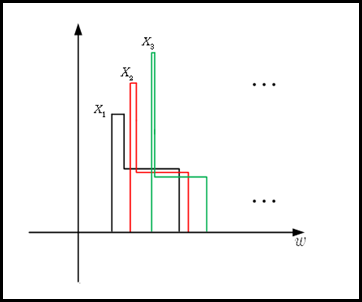
\includegraphics[width=5.03in]{images/basic_UI04} \caption{An example of sequence of random variables that is not bounded but uniformly integrable.}\label{fig:unnamed-chunk-61}
\end{figure}

\section{Big O와 small o (big O and small
o)}\label{big-o-small-o-big-o-and-small-o}

\(x_{n}\)을 무작위 벡터, \(a_{n}\)을 실수라고 하자.

\begin{eqnarray*}
x_{n}\stackrel{n\rightarrow \infty}{=}o(a_{n}) &\Leftrightarrow& \lim_{n\rightarrow\infty}\frac{x_{n}}{a_{n}}=0 \\
&\Leftrightarrow& \frac{x_{n}}{a_{n}}\stackrel{n\rightarrow \infty}{=}o(1)\\
\end{eqnarray*}

\begin{eqnarray*}
x_{n}\stackrel{n\rightarrow \infty}{=}O(a_{n}) &\Leftrightarrow& \text{sup}_{n}|\frac{x_{n}}{a_{n}}| < \infty \\
&\Leftrightarrow& \frac{x_{n}}{a_{n}}\stackrel{n\rightarrow \infty}{=}O(1)\\
\end{eqnarray*}

\section{Big Op와 small op (big Op and small
op)}\label{big-op-small-op-big-op-and-small-op}

이번엔 \(X_{n}\)을 무작위 벡터, \(a_{n}\)을 실수라고 하자.

\begin{eqnarray*}
X_{n}\stackrel{n\rightarrow \infty}{=}o_{p}(a_{n}) &\Leftrightarrow& |\frac{X_{n}}{a_{n}}|\stackrel{P}{\rightarrow}0 \\
&\Leftrightarrow& \frac{X_{n}}{a_{n}}=o_{p}(1)\\
\end{eqnarray*}

\begin{eqnarray*}
X_{n}\stackrel{n\rightarrow \infty}{=}O_{p}(a_{n}) &\Leftrightarrow& \text{sup}_{n} P\{ \frac{X_{n}}{a_{n}}>k\}\stackrel{k\rightarrow\infty}{\rightarrow}0 \\
&\Leftrightarrow& \frac{X_{n}}{a_{n}}\stackrel{n\rightarrow \infty}{=}O_{p}(1)\\
\end{eqnarray*}

\section{절대연속(absolute continuous)}\label{absolute-continuous}

확률변수 \(X_{1}\), \(X_{2}\)가 있을 때 \(X_{1}\)이 \(X_{2}\)에 대해
\textbf{절대연속(absolute continuous)}하다는 것은(정확히 얘기하면
\(X_{1}\)의 분포가 \(X_{2}\)의 분포에 대해 절대연속이다) 적당한 집합
\(F\)에 대해 \(P(X_{2}\in F)=0\)이 \(P(X_{1}\in F)=0\)임을 내포하는 것과
동치이다.

\section{대수의 법칙(law of large numbers)}\label{-law-of-large-numbers}

\BeginKnitrBlock{proposition}[대수의 약법칙과 대수의 강법칙]
\protect\hypertarget{prp:unnamed-chunk-62}{}{\label{prp:unnamed-chunk-62}
\iffalse (대수의 약법칙과 대수의 강법칙) \fi{} }\textbf{대수의
약법칙(weak law of large numbers, WLLN)}은 \(\bar{X}_{n}\)이 \(\mu\)에
확률수렴하는 것이고, \textbf{대수의 강법칙(strong law of large numbers,
SLLN)}은 \(\bar{X}_{n}\)이 \(\mu\)에 거의 확실한 수렴을 하는 것이다.
\EndKnitrBlock{proposition}

\chapter{확률과정론}\label{stoprocess}

참고할만한 책으로 \citep{Lindgren2012}가 있다.

\section{확률과정이란?(stochastic process)}\label{stochastic-process}

\begin{figure}

{\centering 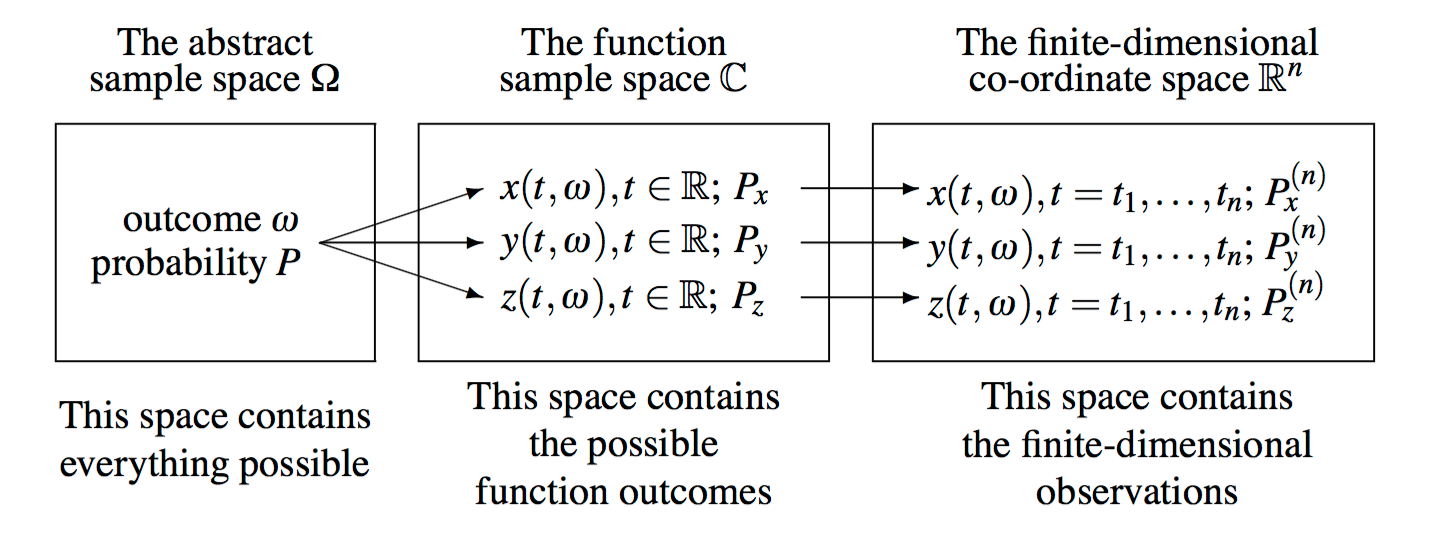
\includegraphics[width=19.94in]{images/basic_stprocess} 

}

\caption{Overview of the threee types of worlds in which our processes live.}\label{fig:unnamed-chunk-63}
\end{figure}

\textbf{확률과정(stochastic process)}란 확률공간에서 정의되는
확률변수들의 모임 \(\{ Z, t \in T\}\)라고 할 수 있다. 이 때
\(T=(-\infty, \infty)\) 등과 같이 연속된 구간의 형태를 갖는 경우를
\textbf{연속형 확률과정(continuous stochastic process)},
\(T=\{ 0, \pm 1, \pm 2 , \ldots\}\) 등과 같이 이산 구간일 경우는
\textbf{이산형 확률과정(discrete stochastic process)}라고 한다.

\section{확률과정에서의 연속성(continuity of stochastic
process)}\label{-continuity-of-stochastic-process}

\subsection{연속표본경로(continuous sample
paths)}\label{continuous-sample-paths}

\BeginKnitrBlock{definition}[연속표본경로]
\protect\hypertarget{def:unnamed-chunk-64}{}{\label{def:unnamed-chunk-64}
\iffalse (연속표본경로) \fi{} }과정 \(X\)가 \(t_{0}\)에서 연속이라 함은
\[\text{For almost all }\omega, t \rightarrow t_{0} \text{ implies } X(t,\omega) \rightarrow X(t_{0},\omega)\]
를 의미한다. 과정 \(X\)가 연속이라 함은
\[\text{For almost all }\omega, X(\cdot, \omega) \text{ is a continuous function}\]
임을 의미한다.
\EndKnitrBlock{definition}

\section{브라운운동(Brownian motion)}\label{brownian-motion}

\BeginKnitrBlock{definition}[저차원에서의 브라운운동]
\protect\hypertarget{def:unnamed-chunk-65}{}{\label{def:unnamed-chunk-65}
\iffalse (저차원에서의 브라운운동) \fi{} }실수값을 갖는 확률과정
\(\{ B(t) : t\geq 0\}\)이 다음 조건들을 만족할 때

\begin{enumerate}
\def\labelenumi{\arabic{enumi}.}
\item
  \(B(0)=x\)
\item
  그 과정이 독립 증분(independent increment)을 갖는다. 즉 모든 시간
  \(0 \leq t_{1} \leq t_{2} \leq \cdots \leq t_{n}\)에 대해 증분
  \(B(t_{n})-B_(t_{n-1}),\ldots, B(t_{2})-B_(t_{1})\)이 독립 확률변수다.
\item
  모든 \(t \geq 0\)과 \(h > 0\)에 대해 증분 이 정규분포를 따른다.
  \[B(t+h)-B(t) \sim \mathcal{N}(0,h).\]
\item
  함수 \(t \rightarrow B(t)\)가 연속이다.
\end{enumerate}

\(x\in\mathbb{R}\)에서 시작하는 (선형) \textbf{브라운운동(Brownian
motion)}이라고 한다. 특별히 \(x=0\)일 때 \(\{ B(t): t\geq 0\}\)을 정규
브라운운동(standard Brownian motion)이라고 부른다.
\EndKnitrBlock{definition}

브라운운동의 정의는 나중에 공간과정에도 잠시 나올 것이다.

\subsection{분수 브라운운동(fractional Brownian
motion)}\label{-fractional-brownian-motion}

\textbf{분수 브라운운동(fractional Brownian motion)}이란 fractional
derivative (또는 fractional integral) of Brownian motion을 일컫는
말이다.

\section{마팅게일(martingale)}\label{martingale}

\BeginKnitrBlock{definition}[마팅게일]
\protect\hypertarget{def:unnamed-chunk-66}{}{\label{def:unnamed-chunk-66}
\iffalse (마팅게일) \fi{} }확률과정 \(\{X_{n}\}\)가

\begin{enumerate}
\def\labelenumi{\arabic{enumi}.}
\item
  \(E |X_{n}| < \infty\)
\item
  \(X_{n}\) is adpated to \(\mathcal{F}_{n}\). (즉 모든 \(n\)에 대해
  \(X_{n}\in\mathcal{F}_{n}\))
\item
  \(E(X_{n+1}|\mathcal{F}_{n})=X_{n}, \text{ for all } n\)
\end{enumerate}

을 만족할 때, 이 확률과정을 filtration \(\mathcal{F}_{n}\)에 대한
\textbf{마팅게일(martingale)}이라 부른다.
\EndKnitrBlock{definition}

\section{마르코프 체인(Markov chain)}\label{-markov-chain}

\BeginKnitrBlock{definition}[마르코프 체인]
\protect\hypertarget{def:unnamed-chunk-67}{}{\label{def:unnamed-chunk-67}
\iffalse (마르코프 체인) \fi{} }\textbf{마르코프 체인(Markov chain)}이란

\[P(X_{n+1}=X|X_{1}=x_{1}, X_{2}=x_{2}, \ldots , X_{n}=x_{n})=P(X_{n+1}=x|X_{n}=x_{n})\]

을 만족하는 확률변수들의 수열 \(X_{1},X_{2},\ldots\)를 일컫는다.
여기서\(x_{i}\)들은 countable set \(S\)에서 뽑힌 값들이며 \(S\)를 체인의
state space라고 부른다.
\EndKnitrBlock{definition}

\section{R 예제(R-stoprocess)}\label{r-r-stoprocess}

\chapter{회귀분석}\label{reg}

AIC, AICc, BIC

\section{선형모형(linear model)}\label{linear-model}

이 절의 내용은 \citep{Yee2015}를 따른다.

\chapter{벌점화 및 축소방법}\label{penalshrink}

때때로 설명변수들이 너무 많아져 특이 관찰값보다도 많아지는 경우가
존재한다. 이런 경우에는 전체 모형을 적합할 경우 prediction interval이
커지고 최소제곱 추정량이 유일하지 않을 수도 있는 등 문제점들이 생기게
된다. 이런 문제점들을 해결하는 방법들을
\textbf{벌점화(penalization)}라고 한다.

최소제곱 추정량은 \((X^{T}X)^{-1}\)에 depend하므로 만약
\((X^{T}X)^{-1}\)이 비정칙(singular)이거나 거의 비정칙일 때
\(\beta_{LS}\)를 계산하는 데 어려움을 겪을 수 있다. 이런 경우에 \(X\)에
약간의 변화만 있어도 \((X^{T}X)^{-1}\)은 크게 달라지게 된다. 이 때
최소제곱 추정량 \(\hat{beta}_{LS}\)는 training data에 적합할 때에는 큰
문제가 되지 않으나 test data에 적합할 때에는 문제가 생길 수도 있다.

\section{능형회귀(ridge regression)}\label{ridge-regression}

앞서 말한 문제점의 한 가지 해결방법으로 추정량의 불편성을 약간 깨는
방법이 있다. \citep{Hoerl1970}은 \(X^{T}X\)에 작은 상수값 \(\lambda\)를
더해 역을 취해 추정량의 불안정성을 해결할 수 있다고 생각하고 다음과 같은
추정량을 제안하였다.
\[\hat{\beta}_{ridge}=(X^{T}X+\lambda I_{p})^{-1}X^{T}Y.\] 이를
\textbf{능형회귀(ridge regression)} 추정량이라고 부른다. 참고로
수학에서는 이 방법을
\href{https://en.wikipedia.org/wiki/Tikhonov_regularization}{Tikhonov
regularization}이라고 부른다.

\(\hat{\beta}_{ridge}\)는 다음 벌점화제곱합
\[\hat{\beta}^{rodge}=\text{arg}\min_{\beta}\{\sum_{i=1}^{n}(y_{i}-\beta_{0}-\sum_{j=1}^{p}x_{ij}\beta_{j})^{2}+\lambda\sum_{j=1}^{p}\beta_{j}^{2}\}\]
을 최소화하여 얻을 수 있다. 또 다른 표현으로는
\[\hat{\beta}^{rodge}=\text{arg}\min_{\beta}\sum_{i=1}^{n}(y_{i}-\beta_{0}-\sum_{j=1}^{p}x_{ij}\beta_{j})^{2}\text{ for some } t, \sum_{j=1}^{p}\beta_{j}^{2}<t^{2}\]
로도 쓸 수 있다.

벌점화 항을 살펴보면, \(\lambda\)는 미리 선택된 상수(constant)에 벡터
\(\beta\)의 제곱합이 곱해진 형태이다. 이는 \(\beta_{j}\)가 큰 값을
가지면 페널티를 주겠다는 뜻이다. \(\beta_{j}\)가 0에 가까울수록 벌점화
항은 작을 것이다.

\subsection{능형회귀의 기하학적 해석(geometrical interpretation of ridge
regression)}\label{--geometrical-interpretation-of-ridge-regression}

\begin{figure}

{\centering 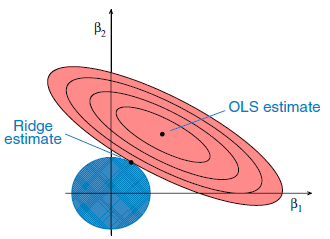
\includegraphics[width=4.58in]{images/basic_ridge} 

}

\caption{Geometric interpretation of ridge regression.}\label{fig:unnamed-chunk-68}
\end{figure}

\(p=2\)인 경우를 생각해보자. 등고선이 있는 붉은색 타원이 residual sum of
squares (RSS)에 해당하며 가장 안쪽에 있는 원이 작은 RSS를 가지고 그
중심에 \(\hat{\beta}_{OLS}\)가 있다. \(p=2\)일 때 능형회귀의 제약조건은
원에 대응된다. 능형회귀의 해는 타원과 원이 만나는 지점이 될 것이다.

여기서 penalty term과 RSS 사이에는 trade-off가 있다고 한다.

\subsection{능형회귀추정량의 성질들(properties of ridge
estimator)}\label{-properties-of-ridge-estimator}

\subsection{SVD를 이용한 능형회귀 해의 계산(computing the ridge
solutions via the
SVD)}\label{svd----computing-the-ridge-solutions-via-the-svd}

능형회귀의 해

\[\hat{\beta}_{ridge}=(X^{T}X+\lambda I_{p})^{-1}X^{T}Y\]

를 다시 상기해보자. \(\hat{\beta}_{ridge}\)를 구할 때 피하고 싶은
역행렬의 계산이 있다. 수치적으로 불안정할 뿐더러 계산량이 대략
\(\mathcal{O}(p^{3})\) 정도 된다. 역행렬의 계산을 피할 수 있는 방법으로
SVD를 이용하는 방법이 있다. 즉

\[X=UDV^{T}\]

임을 이용해 해를 계산하는 것이다.

\section{라쏘(LASSO)}\label{lasso}

능형회귀는 축소 추정치를 주지만 변수선택은 하지 않는다. 따라서 고차원
자료의 경우 최종 모형에 대한 해석이 그리 용이하지 않다.

\chapter{일반화선형모형}\label{glm}

\citep{Nelder1972}는 몇가지 중요한 회귀분석 모형들을 통합한 개념인
\textbf{일반화선형모형(generalized linear model, GLM)}을 발표하였다. 이
논문에서 \textbf{포아송 회귀(Poisson regression)}와 \textbf{로지스틱
회귀(logistic regression)}가 GLM의 특수한 경우임을 보이고 추정을 위해
\textbf{반복재가중최소제곱(iteratively reweighted least squares, IRLS)}
알고리즘이 사용될 수 있음을 보였다.

\section{일반화선형모형의 기본(GLM basics)}\label{-glm-basics}

\section{벡터 일반화선형모형(vector generalized linear
models)}\label{-vector-generalized-linear-models}

이 절의 내용은 \citep{Yee2015}를 따른다.

\section{일반화선형모형의 한계점(limations of
glm)}\label{-limations-of-glm}

\citep{Yee2015}에 의하면 GLM은 잘 알려진 지수족 내의 일차원 분포에서만
잘 적용된다는 한계점을 가지고 있다.

\chapter{일반화가법모형}\label{gam}

일반화가법모형에 대한 참고문헌으로는 \citep{Wood2006}이 있다. 최근에
나온 좋은 책으로는 \citep{Yee2015}가 있으며 이 책은 주로 \textbf{벡터
일반화선형모형(vector genearlized linear model, VGLMs)} 및 \textbf{벡터
일반화가법모형(vector generalized addtive model, VGAMs)}에 초점을 맞추고
있고 R 코드를 포함하고 있다.

\section{가법모형들(additive models)}\label{additive-models}

회귀분석의 \textbf{가법모형(additive model)}은
\[E[Y|\mathbf{X}=\mathbf{x}]=\alpha+\sum_{j=1}^{p}f_{j}(x_j)\] 로
표현한다. 선형모형은 \(f_{j}(x_{j})=\beta_{j}x_{j}\)인 가법모형의 특별한
경우이다. \(f_{j}\)는 임의의 비선형 함수도 될 수 있다는 점에서
가법모형이 좀 더 일반적인 형태의 모형이라고 할 수 있다.

\section{퇴각 적합화(backfitting)}\label{-backfitting}

\textbf{퇴각 적합화(backfitting)}는 \textbf{가우스-자이델
방법(Gauss-Seidel method)}이라고도 불리는 방법으로, GAM을 적합하기 위한
단순하면서도 아름다운 방법이다. 이 알고리즘의 기본 아이디어는 가법모형의
각 smooth component들에 대해 iteratively하게 가법모형의 smooth partial
residuals를 계산하는 것이다.

다음과 같은 가법모형에서 추정을 하고 싶다고 가정하자.
\[y_{i}=\alpha + \sum_{j=1}^{m}f_{j}(x_{ji})+\epsilon_{i},\] 여기서
\(f_{i}\)는 부드러운 함수들(smooth functions)이며 공변량 \(x_{j}\)는
때때로 벡터이기도 하다. \(\hat{\mathbf{f}}_{j}\)를 \(i\)째 원소의
추정값이 \(f_{j}(x_{ji})\)인 벡터라고 하자. 그러면 기본적인 퇴각 적합화
알고리즘은 다음과 같다.

\begin{enumerate}
\def\labelenumi{\arabic{enumi}.}
\item
  Set \(\alpha=\bar{y}\) and \(\hat{\mathbf{f}}_{j}=\mathbf{0}\) for
  \(j=1,\ldots , m\).
\item
  Repeat step 3 to 5 until teh estimates
  \(\hat{\mathbf{f}}_{j}=\mathbf{0}\) stop changing.
\item
  For \(j=1,\ldots ,m\), repeat steps 4 and 5.
\item
  Calculate partial residuals:
  \[\mathbf{e}_{P}^{j}=\mathbf{y}-\hat{\alpha}-\sum_{k\neq j}\hat{\mathbf{f}}_{k}.\]
\item
  Set \(\hat{\mathbf{f}}_{j}\) equal to the result of smoothing
  \(e_{p}^{j}\) with respect to \(x_{j}\).
\end{enumerate}

\section{R 예제(R-gam)}\label{r-r-gam}

알고리즘을 짜면 다음과 같다.

\begin{Shaded}
\begin{Highlighting}[]
\NormalTok{f<-x*}\DecValTok{0}\NormalTok{;alpha<-}\KeywordTok{mean}\NormalTok{(y);ok <-}\StringTok{ }\OtherTok{TRUE}
\NormalTok{while (ok) \{ }\CommentTok{# backfitting loop}
  \NormalTok{for (i in }\DecValTok{1}\NormalTok{:m) \{ }\CommentTok{# loop through the smooth terms}
    \NormalTok{ep <-}\StringTok{ }\NormalTok{y -}\StringTok{ }\KeywordTok{rowSums}\NormalTok{(f[,-i]) -}\StringTok{ }\NormalTok{alpha}
    \NormalTok{b <-}\StringTok{ }\KeywordTok{smooth.spline}\NormalTok{(x[,i],ep,}\DataTypeTok{df=}\NormalTok{edf[i])}
    \NormalTok{f[,i] <-}\StringTok{ }\KeywordTok{predict}\NormalTok{(b,x[,i])$y}
  \NormalTok{\}}
  \NormalTok{rss <-}\StringTok{ }\KeywordTok{sum}\NormalTok{((y-}\KeywordTok{rowSums}\NormalTok{(f))ˆ}\DecValTok{2}\NormalTok{)}
  \NormalTok{if (}\KeywordTok{abs}\NormalTok{(rss-rss0)<}\FloatTok{1e-6}\NormalTok{*rss) ok <-}\StringTok{ }\OtherTok{FALSE}
  \NormalTok{rss0 <-}\StringTok{ }\NormalTok{rss}
\NormalTok{\}}
\end{Highlighting}
\end{Shaded}

\chapter{시계열분석}\label{ts}

내용과 표기는 \citep{Shumway2010}를 따른다. \citep{Cryer2008}또한 R
예제가 이쓴 시계열분석 교재로써 참고할 만 하다.

시계열에서 다루는 대부분의 확률모형들은 확률과정을 설명하는 모형이라고
한다. 관측된 시계열은 표본공간의 각 원소에 대응하는 확률과정
\(\{ Z_{t}(\omega), t=1,2,\ldots \}\)의 관측값으로 시간의 함수이며, 이를
확률과정의 \textbf{실현값(realization)} 또는 \textbf{표본통로(sample
path)}라고 부른다. 우리가 과거로 돌아갈 수 있어 반복 관측을 할 수 있다면
현재 관측된 시계열은 무한히 많은 관측 가능한 확률변수들의 모임 중에서
특별히 실현된 하나에 해당된다. 시계열 분석의 가장 큰 특징은 분석의
대상이 되는 자료가 반복 관측될 수 없다는 점이다.

\section{정상시계열(stationary time
series)}\label{stationary-time-series}

다음 설명은
\href{http://www.dodomira.com/2016/04/21/r-시계열-분석-arima/?subscribe=success\#blog_subscription-2}{DODOMIRA}에서
따온 것이다.

안정적인 시계열이란 다음 세 가지 특징을 가진 시계열을 말한다.

\begin{enumerate}
\def\labelenumi{\arabic{enumi}.}
\tightlist
\item
  시간의 추이와 관계 없이 평균이 불변한다.
\end{enumerate}

\begin{figure}

{\centering 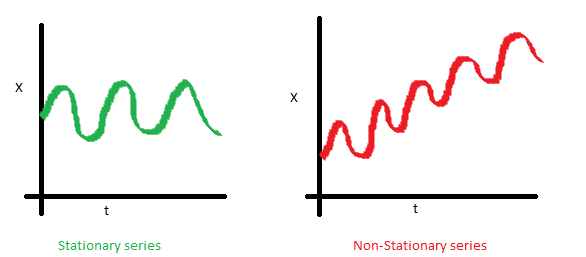
\includegraphics[width=8.14in]{images/basic_mean_nonstationary} 

}

\caption{Time invariant mean.}\label{fig:unnamed-chunk-71}
\end{figure}

\begin{enumerate}
\def\labelenumi{\arabic{enumi}.}
\setcounter{enumi}{1}
\tightlist
\item
  시간의 추이와 관계 없이 분산이 불변한다.
\end{enumerate}

\begin{figure}

{\centering 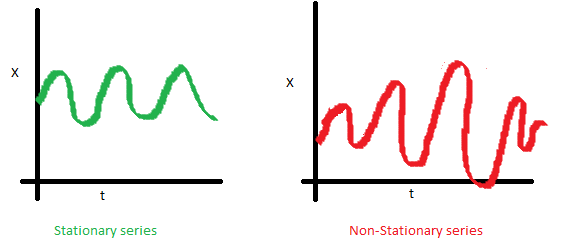
\includegraphics[width=8.01in]{images/basic_var_nonstationary} 

}

\caption{Time invariant variance.}\label{fig:unnamed-chunk-72}
\end{figure}

\begin{enumerate}
\def\labelenumi{\arabic{enumi}.}
\setcounter{enumi}{2}
\tightlist
\item
  시간의 추이와 관계 없이 공분산이 불변한다.
\end{enumerate}

\begin{figure}

{\centering 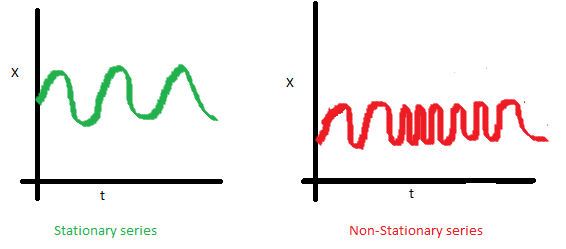
\includegraphics[width=7.86in]{images/basic_cov_nonstationary} 

}

\caption{Time invariant covariance.}\label{fig:unnamed-chunk-73}
\end{figure}

\BeginKnitrBlock{definition}[강정상성]
\protect\hypertarget{def:unnamed-chunk-74}{}{\label{def:unnamed-chunk-74}
\iffalse (강정상성) \fi{} }시계열 \(\{ x_{t}\}\)가 있을 때 두 collection

\[\{ x_{t_{1}}, x_{t_{2}}, \cdots  x_{t_{k}}\}, \{ x_{t_{1+h}}, x_{t_{2+h}}, \cdots  x_{t_{k+h}}\}\]

가 identical하다면, 즉 모든 \(k=1,2,\ldots\), 모든 숫자
\(c_{1},c_{2},\ldots , c_{k}\) 그리고 \(h=0, \pm 1, \pm 2,\ldots\)에
대해

\[P \{ x_{t_{1}} <c_{1}, \ldots , x_{t_{k}} \leq c_{k}\}=P \{ x_{t_{1+h}} <c_{1}, \ldots , x_{t_{k+h}} \leq c_{k}\}\]

일 때 이 시계열을 \textbf{강정상성(strictly stationary)}이라고 한다.
\EndKnitrBlock{definition}

그러나 강정상성의 정의는 대부분의 응용에서 너무 강한 조건인데, 특히
single data set으로부터 강정상성을 assess하기 어렵다고 한다.
시계열에서는 series의 첫 두 moment에만 관련된 약정상성을 생각하여 조건을
부드럽게 한다.

\BeginKnitrBlock{definition}[약정상성]
\protect\hypertarget{def:unnamed-chunk-75}{}{\label{def:unnamed-chunk-75}
\iffalse (약정상성) \fi{} }시계열 \(x_{t}\)가 finite variance를 갖는
process이며

\begin{enumerate}
\def\labelenumi{\arabic{enumi}.}
\item
  평균함수 \(\mu_{t}\)가 상수이며 시간에 따라 변하지 않고
\item
  자기공분산함수 \(\gamma(s,t)\)가 이들의 차이 \(|s-t|\)에만 depend할 때
\end{enumerate}

이 시계열을 \textbf{약정상성(weekly stationary)}이라고 한다.
\EndKnitrBlock{definition}

\BeginKnitrBlock{definition}[자기공분산함수]
\protect\hypertarget{def:unnamed-chunk-76}{}{\label{def:unnamed-chunk-76}
\iffalse (자기공분산함수) \fi{} }정상시계열의
\textbf{자기공분산함수(autocovariance function)}는
\[\gamma(h)=Cov(x_{t+h}, x_{t})=E[(x_{t+h}-\mu)(x_{t}-\mu)]\] 로
정의된다.
\EndKnitrBlock{definition}

\BeginKnitrBlock{definition}[자기상관함수]
\protect\hypertarget{def:unnamed-chunk-77}{}{\label{def:unnamed-chunk-77}
\iffalse (자기상관함수) \fi{} }정상시계열의
\textbf{자기상관함수(autocorrelation function)}는
\[\rho(h)=\frac{\gamma(t+h,t)}{\sqrt{\gamma(t+h,t_h)\gamma(t,t)}}=\frac{\gamma(h)}{\gamma(0)}\]
이다.
\EndKnitrBlock{definition}

\begin{itemize}
\item
  linear process, guassian process
\item
  ACF, PACF, CCF
\end{itemize}

\section{시계열자료의 특성(characteristics of time
series)}\label{-characteristics-of-time-series}

\section{시계열 회귀분석(time series
regression)}\label{-time-series-regression}

\(x_{t},t=1,\ldots ,n\)을 시계열 자료라고 하자. 그리고 이 자료가 다른
투입량 또는 독립적인 시계열 \(z_{t1}, z_{t2}, \ldots ,z_{tq}\)의 영향을
받는다고 하자. 이 가정은 일반적인 회귀분석에서 놓는 가정이다. 이 관계를
회귀분석 모형으로 쓰면

\begin{equation}\label{eq:tsreg}
x_{t}=\beta_{1}z_{t1}+\beta_{2}z_{t2}+\ldots + \beta_{q}z_{tq}+w_{t}
\end{equation}

로 놓을 수 있다. 이 때 \(\beta_{1},\beta_{2}.\ldots , \beta_{q}\)는
알려지지 않은 고정된 회귀계수(regression coefficients)들이고
\(\{ w_{t}\}\)는 i.i.d. 정규분포\((0,\sigma_{w}^{2})\)를 따르는 무작위
오류나 잡음과정(noise process)이라고 놓는다.

선형모형 (\eqref{eq:tsreg})은 일반적으로 벡터
\(\mathcal{z}_{t}=(z_{t1},z_{t2},\ldots , z_{tq})^{T}\),
\(\boldsymbol{\beta}(\beta_{1},\beta_{2},\ldots ,\beta_{q})^{T}\)를 써서
나타낸다. 그러면 (\eqref{eq:tsreg})은

\begin{equation}\label{eq:tsregvec}
x_{t}=\boldsymbol{\beta}^{T}\mathcal{z}_{t}+w_{t}
\end{equation}

으로 간단히 쓸 수 있다. 이 때 알려지지 않은 모수
\(\boldsymbol{\beta}\)의 추정은 다음 식

\begin{equation}\label{eq:tsss}
Q=\sum_{t=1}^{n}w_{t}^{2}=\sum_{t=1}^{n}(x_{t}-\boldsymbol{\beta}^{T}\mathbf{z}_{t})^{2}
\end{equation}

를 \(\beta_{1},\beta_{2},\ldots ,\beta_{q}\)에 대해 풀어 얻을 수 있다.

다시 식 (\eqref{eq:tsreg})를 행렬 형태로 바꿔서 풀어보자. \(n\times q\)
행렬
\(Z= [\mathbf{z}_{1} | \mathbf{z}_{2} | \cdots | \mathbf{z}_{n} ]^{T}\)과
\(n \times 1\) 벡터 \(\mathcal{x}=(x_{1},x_{2},\ldots , x_{n})^{T}\),
\(n \times 1\) 오차의 벡터
\(\mathcal{w}=(w_{1},w_{2}, \ldots, w_{n})^{T}\)를 이용해 식
(\eqref{eq:tsss})를

\begin{equation}\label{eq:tsmatrix}
\mathbf{x}=Z\boldsymbol{\beta}+\mathbf{w}
\end{equation}

로 바꿔 쓸 수 있다. 이것을 \textbf{정규방정식(normal equation)}이라고
쓴다. (\eqref{eq:tsmatrix})의 해는 \(Z^{T}Z\)이 nonsingular일 때

\[\hat{\boldsymbol{\beta}}=(Z^{T}Z)^{-1}Z^{T}\mathbf{x}\]

로 얻을 수 있다.

오차 \(w_{t}\)가 정규분포를 따르면, \(\hat{\boldsymbol{\beta}}\)는
\(\beta\)의 최대가능도추정량(maximum likelihood estimator)을 따르며

\[Cov(\hat{\boldsymbol{\beta}})=\sigma_{w}^{2}(\sum_{t=1}^{n}\mathbf{z}_{t}\mathbf{z}_{t}^{T})^{-1}=\sigma_{w}^{2}(Z^{T}Z)^{-1}=\sigma_{w}^{2}C\]

이다. 여기서

\[C=(Z^{T}Z)^{-1}\]

은 나중에 식을 전개하기 위해 미리 정의해 둔다.

(Hilbert spaces and the Projection theorem)

\section{차분(differencing)}\label{differencing}

시계열 자료가 정상성(stationary)을 유지하기 위해서 인접한 시간들에 있는
값들의 차이를 활용하는 경우가 많다. 왜냐면 이는
자기상관(autocorrelation)과도 관련이 있기 때문이다.

\begin{Shaded}
\begin{Highlighting}[]
\KeywordTok{library}\NormalTok{(astsa)}
\NormalTok{fit =}\StringTok{ }\KeywordTok{lm}\NormalTok{(gtemp~}\KeywordTok{time}\NormalTok{(gtemp), }\DataTypeTok{na.action=}\OtherTok{NULL}\NormalTok{) }\CommentTok{# regress gtemp on time}
\KeywordTok{par}\NormalTok{(}\DataTypeTok{mfrow=}\KeywordTok{c}\NormalTok{(}\DecValTok{2}\NormalTok{,}\DecValTok{1}\NormalTok{))}
\KeywordTok{plot}\NormalTok{(}\KeywordTok{resid}\NormalTok{(fit), }\DataTypeTok{type=}\StringTok{"o"}\NormalTok{, }\DataTypeTok{main=}\StringTok{"detrended"}\NormalTok{)}
\KeywordTok{plot}\NormalTok{(}\KeywordTok{diff}\NormalTok{(gtemp), }\DataTypeTok{type=}\StringTok{"o"}\NormalTok{, }\DataTypeTok{main=}\StringTok{"first difference"}\NormalTok{)}
\end{Highlighting}
\end{Shaded}

\begin{figure}

{\centering 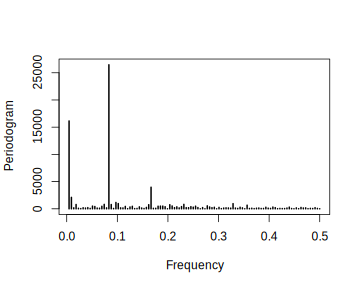
\includegraphics{book_files/figure-latex/unnamed-chunk-78-1} 

}

\caption{Detrended (top) and differenced (bottom) global temperature series.}\label{fig:unnamed-chunk-78}
\end{figure}

\begin{Shaded}
\begin{Highlighting}[]
\KeywordTok{par}\NormalTok{(}\DataTypeTok{mfrow=}\KeywordTok{c}\NormalTok{(}\DecValTok{3}\NormalTok{,}\DecValTok{1}\NormalTok{)) }\CommentTok{# plot ACFs}
\KeywordTok{acf}\NormalTok{(gtemp, }\DecValTok{48}\NormalTok{, }\DataTypeTok{main=}\StringTok{"gtemp"}\NormalTok{)}
\KeywordTok{acf}\NormalTok{(}\KeywordTok{resid}\NormalTok{(fit), }\DecValTok{48}\NormalTok{, }\DataTypeTok{main=}\StringTok{"detrended"}\NormalTok{)}
\KeywordTok{acf}\NormalTok{(}\KeywordTok{diff}\NormalTok{(gtemp), }\DecValTok{48}\NormalTok{, }\DataTypeTok{main=}\StringTok{"first difference"}\NormalTok{)}
\end{Highlighting}
\end{Shaded}

\begin{figure}

{\centering 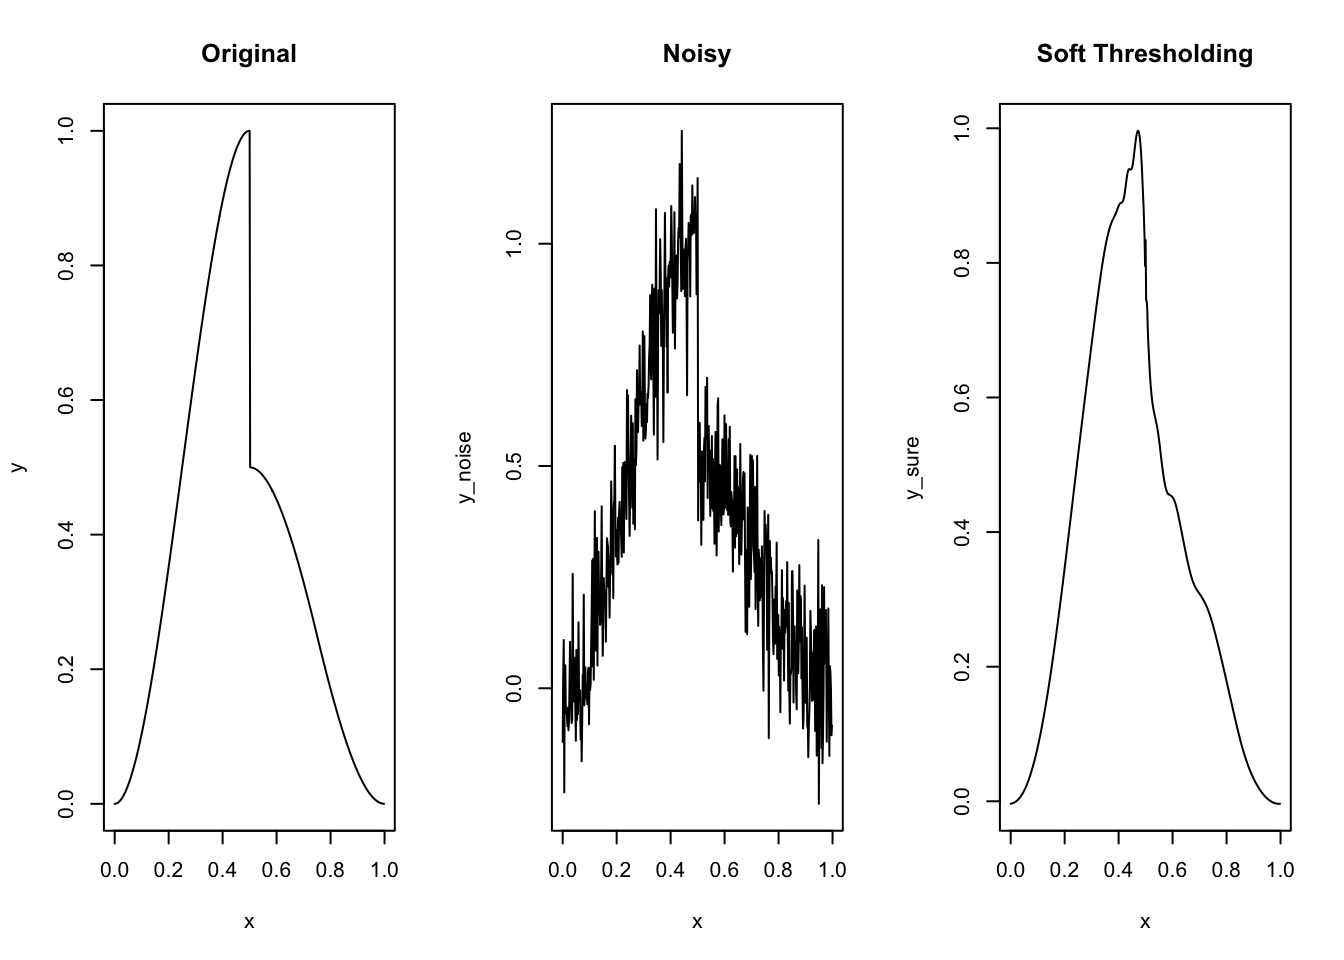
\includegraphics{book_files/figure-latex/unnamed-chunk-79-1} 

}

\caption{Sample ACF (top) detrended sample ACF (middle) and differenced (bottom) global temperature series.}\label{fig:unnamed-chunk-79}
\end{figure}

\section{ARMIA 모델들(ARIMA models)}\label{armia-arima-models}

\subsection{AR 모형(AR models)}\label{ar-ar-models}

이 모형은 현재의 관측값을 과거의 관측값들의 함수형태로 나타내는 것이다.

\BeginKnitrBlock{definition}[자기회귀모형]
\protect\hypertarget{def:unnamed-chunk-80}{}{\label{def:unnamed-chunk-80}
\iffalse (자기회귀모형) \fi{} }\textbf{AR(p)} 차수 p를 갖는
\textbf{자기회귀모형(autoregressive model, AR model)}은
\[x_{t}=\phi_{1}x_{t-1}+\phi_{2}x_{t-2} + \cdots + \phi_{p}x_{t-p}+w_{t}\]
와 같은 형태를 갖는다. 여기서 \(x_{t}\)는 정상과정이며,
\(\phi_{1},\ldots , \phi_{p}\)는 상수이다.
\EndKnitrBlock{definition}

일반적으로 AR과정의 ACF는 지수적으로 감소하며, PACF는 AR과정의 차수에
해당되는 차수 이후에는 0이 되는 성질을 갖고 있다.

\begin{Shaded}
\begin{Highlighting}[]
\KeywordTok{par}\NormalTok{(}\DataTypeTok{mfrow=}\KeywordTok{c}\NormalTok{(}\DecValTok{3}\NormalTok{,}\DecValTok{2}\NormalTok{))}
\NormalTok{ARsim01 <-}\StringTok{ }\KeywordTok{arima.sim}\NormalTok{(}\KeywordTok{list}\NormalTok{(}\DataTypeTok{order=}\KeywordTok{c}\NormalTok{(}\DecValTok{1}\NormalTok{,}\DecValTok{0}\NormalTok{,}\DecValTok{0}\NormalTok{), }\DataTypeTok{ar=}\NormalTok{.}\DecValTok{9}\NormalTok{), }\DataTypeTok{n=}\DecValTok{100}\NormalTok{)}
\NormalTok{ARsim02 <-}\StringTok{ }\KeywordTok{arima.sim}\NormalTok{(}\KeywordTok{list}\NormalTok{(}\DataTypeTok{order=}\KeywordTok{c}\NormalTok{(}\DecValTok{1}\NormalTok{,}\DecValTok{0}\NormalTok{,}\DecValTok{0}\NormalTok{), }\DataTypeTok{ar=}\NormalTok{-.}\DecValTok{9}\NormalTok{), }\DataTypeTok{n=}\DecValTok{100}\NormalTok{)}
\KeywordTok{plot}\NormalTok{(ARsim01, }\DataTypeTok{ylab=}\StringTok{"x"}\NormalTok{, }\DataTypeTok{main=}\NormalTok{(}\KeywordTok{expression}\NormalTok{(}\KeywordTok{AR}\NormalTok{(}\DecValTok{1}\NormalTok{)~}\ErrorTok{~~}\NormalTok{phi==+.}\DecValTok{9}\NormalTok{)))}
\KeywordTok{plot}\NormalTok{(ARsim02, }\DataTypeTok{ylab=}\StringTok{"x"}\NormalTok{, }\DataTypeTok{main=}\NormalTok{(}\KeywordTok{expression}\NormalTok{(}\KeywordTok{AR}\NormalTok{(}\DecValTok{1}\NormalTok{)~}\ErrorTok{~~}\NormalTok{phi==-.}\DecValTok{9}\NormalTok{)))}
\KeywordTok{acf}\NormalTok{(ARsim01); }\KeywordTok{acf}\NormalTok{(ARsim02); }\KeywordTok{pacf}\NormalTok{(ARsim01); }\KeywordTok{pacf}\NormalTok{(ARsim02)}
\end{Highlighting}
\end{Shaded}

\begin{figure}

{\centering 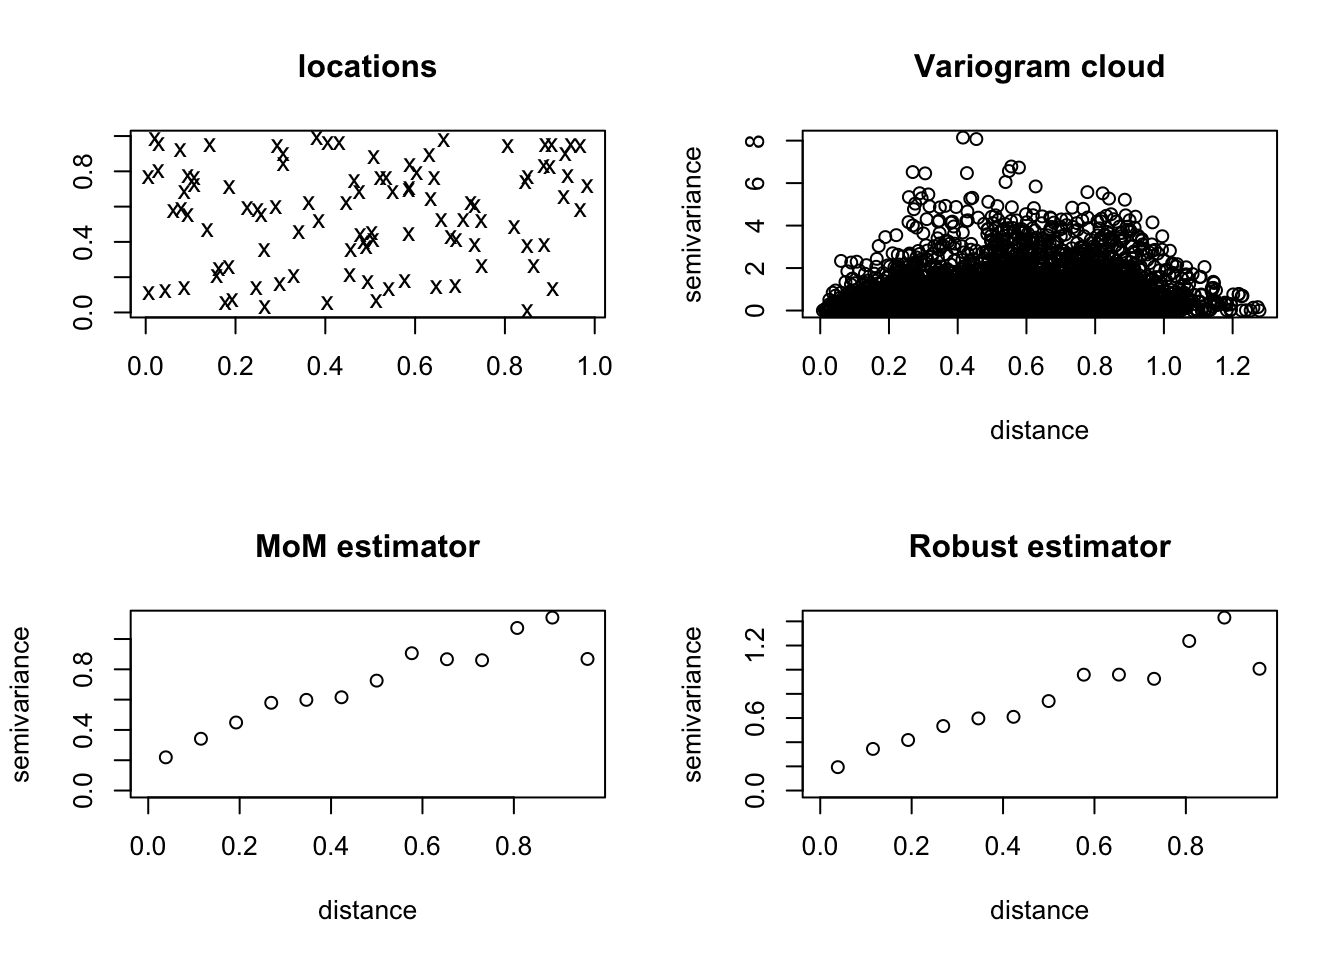
\includegraphics{book_files/figure-latex/unnamed-chunk-81-1} 

}

\caption{Simulated AR model.}\label{fig:unnamed-chunk-81}
\end{figure}

\subsection{MA 모형(MA models)}\label{ma-ma-models}

MA과정의 PACF는 AR과정의 ACF 형태와, MA과정의 ACF는 AR과정의 PACF 형태와
같다.

\begin{Shaded}
\begin{Highlighting}[]
\KeywordTok{par}\NormalTok{(}\DataTypeTok{mfrow=}\KeywordTok{c}\NormalTok{(}\DecValTok{3}\NormalTok{,}\DecValTok{2}\NormalTok{))   }
\NormalTok{MAsim01 <-}\StringTok{ }\KeywordTok{arima.sim}\NormalTok{(}\KeywordTok{list}\NormalTok{(}\DataTypeTok{order=}\KeywordTok{c}\NormalTok{(}\DecValTok{0}\NormalTok{,}\DecValTok{0}\NormalTok{,}\DecValTok{1}\NormalTok{), }\DataTypeTok{ma=}\NormalTok{.}\DecValTok{5}\NormalTok{), }\DataTypeTok{n=}\DecValTok{100}\NormalTok{)}
\NormalTok{MAsim02 <-}\StringTok{ }\KeywordTok{arima.sim}\NormalTok{(}\KeywordTok{list}\NormalTok{(}\DataTypeTok{order=}\KeywordTok{c}\NormalTok{(}\DecValTok{0}\NormalTok{,}\DecValTok{0}\NormalTok{,}\DecValTok{1}\NormalTok{), }\DataTypeTok{ma=}\NormalTok{-.}\DecValTok{5}\NormalTok{), }\DataTypeTok{n=}\DecValTok{100}\NormalTok{)}
\KeywordTok{plot}\NormalTok{(MAsim01, }\DataTypeTok{ylab=}\StringTok{"x"}\NormalTok{, }\DataTypeTok{main=}\NormalTok{(}\KeywordTok{expression}\NormalTok{(}\KeywordTok{MA}\NormalTok{(}\DecValTok{1}\NormalTok{)~}\ErrorTok{~~}\NormalTok{theta==+.}\DecValTok{5}\NormalTok{)))    }
\KeywordTok{plot}\NormalTok{(MAsim02, }\DataTypeTok{ylab=}\StringTok{"x"}\NormalTok{,}\DataTypeTok{main=}\NormalTok{(}\KeywordTok{expression}\NormalTok{(}\KeywordTok{MA}\NormalTok{(}\DecValTok{1}\NormalTok{)~}\ErrorTok{~~}\NormalTok{theta==-.}\DecValTok{5}\NormalTok{))) }
\KeywordTok{acf}\NormalTok{(MAsim01); }\KeywordTok{acf}\NormalTok{(MAsim02); }\KeywordTok{pacf}\NormalTok{(MAsim01); }\KeywordTok{pacf}\NormalTok{(MAsim02)}
\end{Highlighting}
\end{Shaded}

\begin{figure}

{\centering 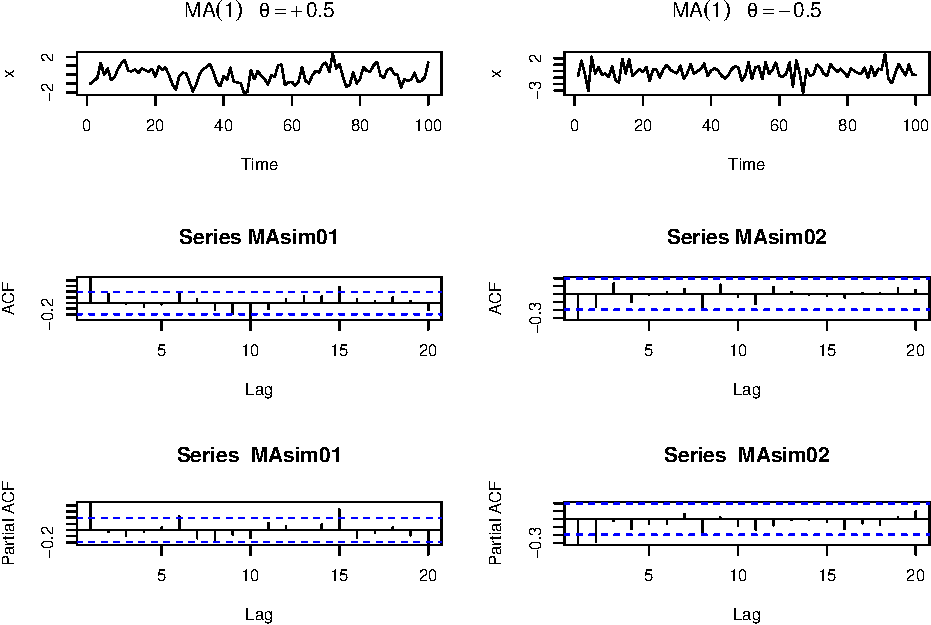
\includegraphics{book_files/figure-latex/unnamed-chunk-82-1} 

}

\caption{Simulated MA model.}\label{fig:unnamed-chunk-82}
\end{figure}

\subsection{ARMA 모형(ARMA models)}\label{arma-arma-models}

\subsection{ARIMA 모형(ARIMA models)}\label{arima-arima-models}

\section{계절성이 있는 ARIMA 모델링(seasonal ARIMA
models)}\label{--arima-seasonal-arima-models}

시계열이 일정한 계절적인 주기를 가지고 변할 때 사용하는 분석 방법으로는
삼각함수 또는 지시함수를 이용한 회귀모형, 계절형 지수평활법 등이 있다.
이러한 방법들은 계절형 시계열이 \[x_{t}=T_{t}+S_{t}+C_{t}+I_{t}\] 와
같이 서로 독립적인 여러 성분들로 구성되어 있을 때 사용 가능하다고 한다.

\begin{itemize}
\item
  \(T_{t}\): 추세성분
\item
  \(S_{t}\): 계절성분
\item
  \(C_{t}\): 순환성분
\item
  \(I_{t}\): 불규칙성분
\end{itemize}

각 성분들은 회귀분석 또는 이동평균법 등을 이용한 전통적인 분해법에 의해
분석할 수 있다. 그러나 이러한 분석법은 시계열을 구성하고 있는 성분들이
결정적이며 서로 독립이라는 가정 하에서 출발하고 있는데, 우리가 접하는
시계열들은 그 구성성분들이 확률적이거나 다른 성분들과 상관이 있는 경우가
많다. 이러한 경우에는 확률적 분석 방법인 ARIMA를 이용한 분석을 한다.

\section{Coherency (section 3.9)}\label{coherency-section-3.9}

\textbf{결맞음(coherency)} 분석은 두 자료의 관계를 quantify하기 위해
많이들 사용한다. 신호 사이의 결맞음 추정은 중요햐며

\section{Self-Similar Process}\label{self-similar-process}

\chapter{전이함수모형}\label{transfer}

시차회귀분석(lagged regression)

입력시계열과 출력시계열로 사용되는 시계열 사이의 관계를 회귀모형의
형태로 표현한 것을 \textbf{전이함수(transfer function)}라고 하며, 이
떄의 모형을 \textbf{전이함수모형(transfer function model)}이라고 한다.
일반적으로 전이함수 모형은 입력시계열이 출력시계열에는 영향을 미치나
반대의 영향은 없다는 가정 하에서 사용한다. 만약 출력시계열도
입력시계열에 영향을 미치는 경우에는 전이함수 모형 대신 벡터 ARIMA 모형을
이용한 분석을 한다.

\begin{equation}\label{eq:lagreg}
y_{t}=\sum_{j=0}^{\infty}\alpha_{j}x_{t-j}+\eta_{t}=\alpha(B)x_{t}+\eta_{t}
\end{equation}

라고 모형을 세우자. 이 때 \(x_{t-j}\)는 입력시계열, \(\eta_{t}\)는
잡음과정이 되며 \[\alpha(B)=\sum_{j=0}^{\infty}\alpha_{j}B^{j}\] 는
전이함수가 된다. 이 때 \(\alpha_{j}\)를 \textbf{충격반응가중값(impulse
response weight)}이라고 부른다.

Box와 Jenkins에 따르면, \(x_{t}\)와 \(\eta_{t}\)에 ARIMA모형을 적합한다.
이 때 \[\phi(B)x_{t}=\theta(B)w_{t} \text{ and }\]
\[\phi_{\eta}(B)\eta_{t}=\theta_{\eta}(B)z_{t}\] 로 표현할 수 있다. 이
때

\begin{itemize}
\tightlist
\item
  \(w_{t},z_{t}\)는 독립이고 분산이 \(\sigma_{w}^{2}\),
  \(\sigma_{z}^{2}\)인 백색잡음과정이다. Box와 Jenkins는
  \(\alpha_{j}, j=1,2,\ldots\)의 형태로 systematic patteren들이 관찰될
  수 있고 이들을 a ratio of polynomials involving a small number of
  coefficients, along with a specified delay \(d\)로 표현할 수 있다고
  한다. 따라서
\end{itemize}

\[\alpha(B)=\frac{\delta (B)B^{d}}{\omega(B)}\] 로 표현할 수 있고(이렇게
표현하면 추정해야 할 모수의 숫자를 줄일 수 있다고 한다), 여기서
\[\omega(B)=1-\omega_{1}B-\omega_{2}B^{2}-\cdots -\omega_{r}B^{r}\] 이며
\[\delta(B)=\delta_{0}+\delta_{1}B+\cdots +\delta_{s}B^{s}\] 들이
지시연산자가 된다. 식 (\eqref{eq:lagreg})를 정리하면
\[\tilde{y}_{t}=\frac{\phi(B)}{\theta(B)}y_{t}=\alpha(B)w_{t}+\frac{\phi(B)}{\theta(B)}\eta_{t}=\alpha(B)w_{t}+\tilde{\eta}_{t}\]
를 얻게 된다. 이 때

\begin{itemize}
\item
  \(\alpha(B)=\sum_{j=0}^{\infty}\alpha_{j}B^{j}\): 전이함수
\item
  \(\tilde{\eta}_{t}\): 변환된 잡음으로 \(w_{t}\)와 독립
\item
  \(\frac{\phi(B)}{\theta(B)}\): \textbf{선형필터(linear filter)}라 부름
\item
  \(w_{t}\): 사전백색화된 input series
\item
  \(\tilde{y}_{t}\): 변환된 output series
\end{itemize}

전이함수모형의 기본 가정은 입력시계열과 반응시계열이 모두
정상시계열이라는 것이다. 따라서 먼저 분석에 사용될 시계열들이 정상성을
갖는지 여부를 판단해야 한다.

\section{안정성과 인과성(stability and
causality)}\label{-stability-and-causality}

(조신섭 교수님 책 참고)

\section{교차상관함수(cross-covariance
function)}\label{cross-covariance-function}

전이함수의 형태를 식별하기 위해서는 충격반응가중값을 먼저 구해야 하는데,
이를 위해 두 개의 시계열 사이의 상관의 정도와 방향을 나타내는
교차상관함수를 이용한다.

\BeginKnitrBlock{definition}[교차상관함수]
\protect\hypertarget{def:unnamed-chunk-83}{}{\label{def:unnamed-chunk-83}
\iffalse (교차상관함수) \fi{} }정상인 두 시계열 \(X_{t}\)와 \(Y_{t}\)
사이의 교차상관함수는
\[\gamma_{XY}(t)=E[(X_{t}-\mu_{X})(Y_{t+k}-\mu_{Y})], \qquad{k=0,\pm 1, \pm 2, \ldots}\]
이다. 단 모든 \(t\)에 대해 \(\mu_{X}=E[X_{t}]\),
\(\mu_{Y}=E[Y_{t}]\)이다.
\EndKnitrBlock{definition}

교차상관함수의 성질 중 중요한 것은 \textbf{자기상관함수와는 달리 대칭이
아니라}는 점이다. 따라서 교차상관함수는 자기상관함수와는 달리 상관의
정도와 영향을 미치는 방향을 같이 측정한다는 점이 특징이다.

\BeginKnitrBlock{definition}[교차상관계수]
\protect\hypertarget{def:unnamed-chunk-84}{}{\label{def:unnamed-chunk-84}
\iffalse (교차상관계수) \fi{} }정상인 두 시계열 \(X_{t}\)와 \(Y_{t}\)
사이의 교차상관함수는
\[\rho_{XY}(k)=Corr(X_{t},Y_{t+k})=\frac{\gamma_{XY}(k)}{\sigma_{X}\sigma_{Y}}=\frac{\gamma_{XY}(k)}{\sqrt{\gamma_{X}(0)\gamma_{Y}(0)}}\]
으로 정의한다.
\EndKnitrBlock{definition}

앞선 모형에서 \(\tilde{y}_{t}\)와 \(w_{t}\)의 교차상관계수는
\[\gamma_{\tilde{y} w}(h)=E[\tilde{y}_{t} w_{t}]=E[\sum_{j=0}^{\infty}\alpha_{j}w_{t+h-j}w_{t}]=\sigma_{w}^{2}\alpha_{h}\]
로 쓸 수 있다. 이는 \(j=h\)일 때를 제외하고 백색잡음의 ACF가 0임을
이용하는 것이다. 이 관계식을 보면
\[\hat{\alpha}_{h}=\frac{\hat{\gamma}_{\tilde{y}w}(h)}{\hat{\sigma}_{w}^{2}}\]
임을 유추해 낼 수 있다.

\section{전이함수모형의 적합(fitting transfer function
model)}\label{-fitting-transfer-function-model}

\begin{enumerate}
\def\labelenumi{\arabic{enumi}.}
\item
  먼저 분석에 이용될 시계열들이 정상이라는 가정을 만족하도록 정상화한다.
\item
  전이함수모형의 식별을 위해 시계열을 사전백색화(prewhitening)한다.
\item
  잠정적인 전이함수모형을 추정한다.
\item
  장차를 이용하여 오차모형을 식별하고 추정한다.
\end{enumerate}

\chapter{칼만 필터}\label{kalman}

자연계에서 나타나는 시계열은 많은 경우, 직전의 상태와 밀접하 관계를
갖으면서 끊임없이 변화하는 형태를 보이고 있어 선형모형으로는 예측의
정확도를 높이는 데 한계가 있을 때가 있다. 실제와 닮은 모형이 더
우수하다는 원칙에서 동적모형에 대한 연구와 적용이 예보의 정확성을 높여줄
것이다.

\textbf{칼만필터(kalman filter)}란 공정제어를 위해 칼만(Kalman)이 1960년
제안한 알고리즘으로, 시간의 흐름에 따라 모형식이 변화하는 동적
모형(dynamic model)으로 선형과 비선형의 중간 형태를 지니고 있다고 한다.
예측 문제도 해결하는 등 여러 가지 장점이 있어 경제 에측, 신호 처리, 기상
예보 등 응용 범위가 넓은 동적 모형이라고 한다.

칼만 필터 모형은 다음의 생성 구조로 이루어진다.

\begin{enumerate}
\def\labelenumi{\arabic{enumi}.}
\item
  초기치가 필요하다.
\item
  주어진 \textbf{상태방정식(state equation)}에 의해 전 상태로부터
  내적오차와 합하여 현 상태값이 결정되며,
\item
  주어진 \textbf{출력방정식(output equation)}에 의해 고려된 입력변수값과
  동적회귀계수 역할을 하는 현 상태의 내적과 출력오차의 합 형태로
  관측치가 생성된다는 가정 아래 구성된 모형으로,
\item
  새로운 관측치가 얻어지면, 모형이 \textbf{최신화(updating)}되도록
  알고리즘이 주어져야 한다.
\end{enumerate}

\(F_{t}\), \(G_{t}\), \(W\), \(V\), \(m_{0}\), \(C_{0}\),
\(t=1,2,\ldots,\) 가 주어진 경우 다음의 생성식으로 이루어진 모형식을
칼만필터 모형이라고 한다.

\[\text{(초기 분포) } \theta_{0} \sim \mathcal{N}(m_{0},C_{0})\]
\[\text{(상태방정식) } \theta_{t}=G_{t}\theta_{t-1}+w_{t}, \qquad{w_{t} \sim \mathcal{N}(0,W)}\]
\[\text{(출력방정식) } Y_{t}=F_{t}\theta_{t}+v_{t}, \qquad{v_{t}\sim \mathcal{N}(0,V)}\]

여기에서

\begin{itemize}
\item
  \(\theta_{t}\): \textbf{상태벡터(state vector)}
\item
  \(G_{t}\): \textbf{전이행렬(transition matrix)}
\item
  \(w_{t}\): \textbf{내적오차벡터(innovational error vector)}
\item
  \(Y_{t}\): \textbf{관측치(observation)}
\item
  \(F_{t}\): \textbf{입력벡터(input vector)}로 상태벡터가 관측치에
  영향을 주는 설명변수들로 이루어져있음
\item
  \(v_{t}\): \textbf{출력오차(output error)}
\end{itemize}

\(\theta_{t-1}\)과 \(w_{t}\)는 독립이며, \(\theta_{t}\)는 \(v_{t}\)와
독립이고, 두 오차는 서로 독립이다.

칼만필터 모형은 두 개 이상의 선형식의 모임으로 연결되어 있으므로
전체적으로는 비선형적 특성을 지니고 있고, 각 식은 선형모형이므로 모형의
설명력과 예측력이 우수하며, 이론적 전개가 용이하다.

\BeginKnitrBlock{example}[칼만필터 모형의 예]
\protect\hypertarget{exm:unnamed-chunk-85}{}{\label{exm:unnamed-chunk-85}
\iffalse (칼만필터 모형의 예) \fi{} }시간에 따라 생성되는 종속변수가
하나이며 설명변수가 두 개인 선형모형을 생각해보자.

\begin{enumerate}
\def\labelenumi{\arabic{enumi}.}
\item
  회귀모형은 회귀계수가 미지의 상수인 경우로 정적 모형이다. 즉
  \[Y_{t}=m_{0}+m_{1}X_{1t}+m_{2}X_{2t}+v_{t}\] 인 형태가 된다.
\item
  회귀동적모형은 회귀계수가 시간에 따라 변화하는 경우로 동적모형이다. 즉
  \[Y_{t}=m_{0t}+m_{1t}X_{1t}+m_{2t}X_{2t}+v_{t}\] 인 형태가 되며 각
  회귀계수들을 함수형태로 추정해 주어야 한다.
\item
  회귀동적선형모형은 회귀계수가 전 시점의 회귀계수에 의하여 결정되는
  경우로 회귀동적모형의 특수한 경우가 된다. 예를 들어, 전이행렬이
  단위행렬인 경우(상태벡터가 임의보행인 경우)
  \[Y_{t}=m_{0t}+m_{1t}X_{1t}+m_{2t}X_{2t}+v_{t}\]
\end{enumerate}

그리고

\[
\theta_{t} =
 \begin{pmatrix}
  m_{0t} \\
  m_{1t} \\
  m_{2t} 
 \end{pmatrix}
= 
 \begin{pmatrix}
  1 & 0 & 0 \\
  0 & 1 & 0 \\
  0 & 0 & 1
 \end{pmatrix}
 \begin{pmatrix}
  m_{0,t-1} \\
  m_{1,t-1} \\
  m_{2,t-1} 
 \end{pmatrix} 
+
 \begin{pmatrix}
  w_{0t} \\
  w_{1t} \\
  w_{2t} 
 \end{pmatrix}
\] 이와 같은 형태를 지닌다.
\EndKnitrBlock{example}

\section{칼만필터 모형의 종류(types of Kalman
filter)}\label{--types-of-kalman-filter}

\subsection{은닉 마르코프 모형(hidden Markov
model)}\label{--hidden-markov-model}

오차항이 없는 칼만필터 모형으로 다음과 같다.

\[
\begin{cases}
\mu_{t}=G\mu_{t-1} \\
Y_{t}=F\mu_{t}.\\
\end{cases}
\]

여기서 전이행렬 \(G\)와 출력행렬 \(F\)는 시간에 따라 변화하지 않으므로
상태방정식은 확률과정에서의 상태벡터 \(\mu_{t}\)의 전이행렬이 \(G\)인
마르코프 연쇄로 생각할 수 있다. 관측치 \(Y_{t}\)만 주어져 있고
\(\mu_{t}\)는 모르는 경우 모수 \(G\)와 \(F\)를 추정하여 생성구조를
완성하는 과정을 이룬다. 은닉 마르코프 모형은 범주형 자료에도 적용이
가능하며, 신호처리에 바탕을 두고 있는 음성인식, 영상인식, 문장인식에
널리 사용되고 있는 통계적 기법이다.

\subsection{일차 칼만필터 모형(simple Kalman filter
model)}\label{--simple-kalman-filter-model}

\textbf{일차 칼만필터 모형(simple Kalman filter model)}은 오차항을
포함한 칼만필터 모형 중 가장 간단한 형태로 \(t\) 시점의 상태열이
임의보행과정(random walk)으로 직전 상태값 주위에서 흔들리며 변화할 때
사용한다.

\[
\begin{cases}
\mu_{t}=\mu_{t-1}+w_{t} \\
Y_{t}=\mu_{t}+v_{t}.\\
\end{cases}
\]

\subsection{회귀 칼만필터 모형(regression Kalman filter
model)}\label{--regression-kalman-filter-model}

\textbf{회귀 칼만필터 모형(regression Kalman filter model)}은
입력변수(설명변수)가 있는 경우에 사용하는 동적모형으로 계수(상태열)가
시간에 따라 변화하는 동적 계수가 된다.

\[
\begin{cases}
\theta_{t}=\theta_{t-1}+w_{t} \\
Y_{t}=F_{t}\theta_{t}+v_{t}.\\
\end{cases}
\]

\subsection{일반적 칼만필터 모형(general Kalman filter
model)}\label{--general-kalman-filter-model}

\textbf{일반적 칼만필터 모형(general Kalman filter model)}은 회귀
칼만필터 모형에서 동적 계수가 임의보행이 아닌 경우에 전이행렬을 고려하는
동적모형이다.

\[
\begin{cases}
\theta_{t}=G_{t}\theta_{t-1}+w_{t} \\
Y_{t}=F_{t}\theta_{t}+v_{t}.\\
\end{cases}
\]

\subsection{확장된 칼만필터 모형(extended Kalman filter
model)}\label{--extended-kalman-filter-model}

칼만필터 모형에서 상태방정식과 출력방정식이 선형모형이 아닌 비선형모형인
경우를 \textbf{확장된 칼만필터 모형(extended Kalman filter model)}이라고
한다. 추정과 최시노하는 주어진 식을 선형화하여 해결하며, 시스템에 대한
물리적 이해가 필요하다.

\[
\begin{cases}
\theta_{t}=f(\theta_{t-1},w_{t}) \\
Y_{t}=h(\theta_{t},v_{t})\\
\end{cases}
\]

\section{최신화 알고리즘(updating algorithm)}\label{-updating-algorithm}

\textbf{칼만필터링(Kalman filtering)}은 칼만필터 모형의 상태열
\(\{ \theta_{t}\}\)의 추정에 사용된다. 칼만필터링은 다음의 특징을 지니고
있어 이공계 분야 모델링에 많이 응용된다.

\begin{itemize}
\item
  미지의 상태열 \(\{\theta_{t}\}\)를 추정하는 반복처리과정이다.
\item
  동적처리기법이다. 즉 시간의 흐름에 따라 진행하면서 과거와 현재의
  출력값들을 보고 현재의 상태를 추정해간다.
\item
  평균제곱오차를 최소로 하는 최적 상태열을 추정하는 통계적 이론을
  바탕으로 한다.
\item
  체계적 기법(systematic method)이다. 즉 일단 칼만필터 모형이 만들어지면
  칼만필터 알고리즘을 쉽게 사용할 수 있다.
\item
  나쁜 초기치의 영향이 오래가지 않는다. 즉 로버스트하다.
\item
  프로그래밍이 쉽다.
\end{itemize}

칼만필터링은 다변량 정규분포이론에 근거하며 최적 상태값을 추정하는
아래와 같은 \textbf{동적순환과정(dynamic recursive procedure)}으로
이루어진다. 이를 \textbf{최신화 알고리즘(updating algoritm)}이라고 한다.
\(t=1,2,\ldots\)로 변화시키며

\begin{enumerate}
\def\labelenumi{\arabic{enumi}.}
\item
  \(t-1\)시점까지의 모든 정보 \(D_{t}\)에 의한 \(\theta_{t-1}\)의 분포
  \[\theta_{t-1}|Y_{t-1} \sim \mathcal{N}(m_{t-1},C_{t-1})\]
\item
  \(t\)시점에서의 \(\theta_{t}\)의 사전분포: 상태방정식
  \(\theta_{t}=G_{t}\theta_{t-1}+w_{t}, w_{t} \sim \mathcal{N}(0,W_{t})\)에
  의하여,
  \[\theta_{t}|D_{t-1} = (G_{t}\theta_{t-1}+w_{t})|D_{t-1}\sim \mathcal{N}(a_{t},R_{t})\]
  여기에서 \(a_{t}=G_{t}m_{t-1}, R_{t}=G_{t}C_{t-1}G_{t}'+W_{t}\)이다.
\end{enumerate}

\section{동적선형모형(dynamic linear model)}\label{dynamic-linear-model}

\section{R-예제(R-dlm)}\label{r-r-dlm}

\chapter{스펙트럼 분석}\label{spectral}

이 절의 내용은 \citep{Shumway2010}를 참고하였다.

시간영역의 분석 방법이 자기상관함수 등을 이용해 시간에 따른 상관 정도를
분석하고 변수들 사이의 관계를 가장 잘 설명해 주는 모형을 찾는 데 반해,
진동수영역의 분석 방법은 시계열이 다양한 주기를 갖는 성분들의
선형결합으로 표현될 수 있다는 성질을 이용해 어떤 주기성분이 중요한
역할을 하는지 알아보는 데 초점을 둔다.

진동수영역의 분석에서는 자기공분산의 \textbf{푸리에변환(Fourier
transform)}으로 정의되는 \textbf{스펙트럼(spectrum)}을 추정하여 각
진동수에 대응되는 주기성분들의 선형결합으로 시계열을 표현한다. 즉,
시계열이 긴 주기 또는 짧은 주기를 갖는지를 각 주기성분들의 기여도를
이용하여 설명 및 분석하는 데, 이 기여도를 자기공분산의 형태로 표현하는
것이 \textbf{스펙트럼분석(spectral analysis)}이다.

\section{순환 움직임과 주기성(cyclical behavior and
periodicity)}\label{--cyclical-behavior-and-periodicity}

다음과 같은 주기과정(periodic process)을 생각해보자.
\[x_{t}=A\cos(2\pi\omega t + \phi), \qquad{\text{for } t=0,\pm 1, \pm 2, \ldots,}\]
여기서

\begin{itemize}
\item
  \(\omega\): \textbf{진동수 지수(frequency index)} (단위 시간 당 순환의
  갯수, 일례로 \(\omega=1/50\)이면 50 포인트마다 한 번씩 주기가 돈다는
  뜻이다)
\item
  \(A\): \textbf{진폭(amplitude)} (신호의 높이 결정)
\item
  \(\phi\): \textbf{위상(phase)} (코사인 함수의 시작 지점)
\end{itemize}

이다. 다음과 같은 삼각함수 공식
\(\cos (\alpha \pm \beta)= \cos (\alpha) \cos (\beta) \mp \sin(\alpha)\sin(\beta)\)을
이용하면 위 식은

\begin{equation}\label{eq:periodrp}
x_{t}=U_{1}\cos(2\pi\omega t) + U_{2}\sin(2\pi\omega t)
\end{equation}

가 되며 \(U_{1}=A\cos \phi\), \(U_{2}=-\sin\phi\)는 종종 정규분포를
따르는 확률변수로 취급한다. 그리고 이 때
\(A=\sqrt{U_{1}^{2}+U_{2}^{2}}\), \(\phi=\tan^{-1}(-U_{2}/U_{1})\)이다.
이 사실로부터, \(A\)와 \(\phi\)가 독립인 확률변수면,
\(A^{2}\sim \chi_{2}\), \(\phi \sim \text{Unif}(-\pi, \pi)\)이며
\(U_{1}\)과 \(U_{2}\)는 독립인 표준 정규분포를 따른다.

앞선 랜덤과정(random process)는 진동수 \(\omega\)를 모수로 하여 표현할
수 있다.

\subsection{중첩 주파수(folding frequency)}\label{-folding-frequency}

\subsection{앨리어싱(aliasing)}\label{aliasing}

\begin{figure}

{\centering 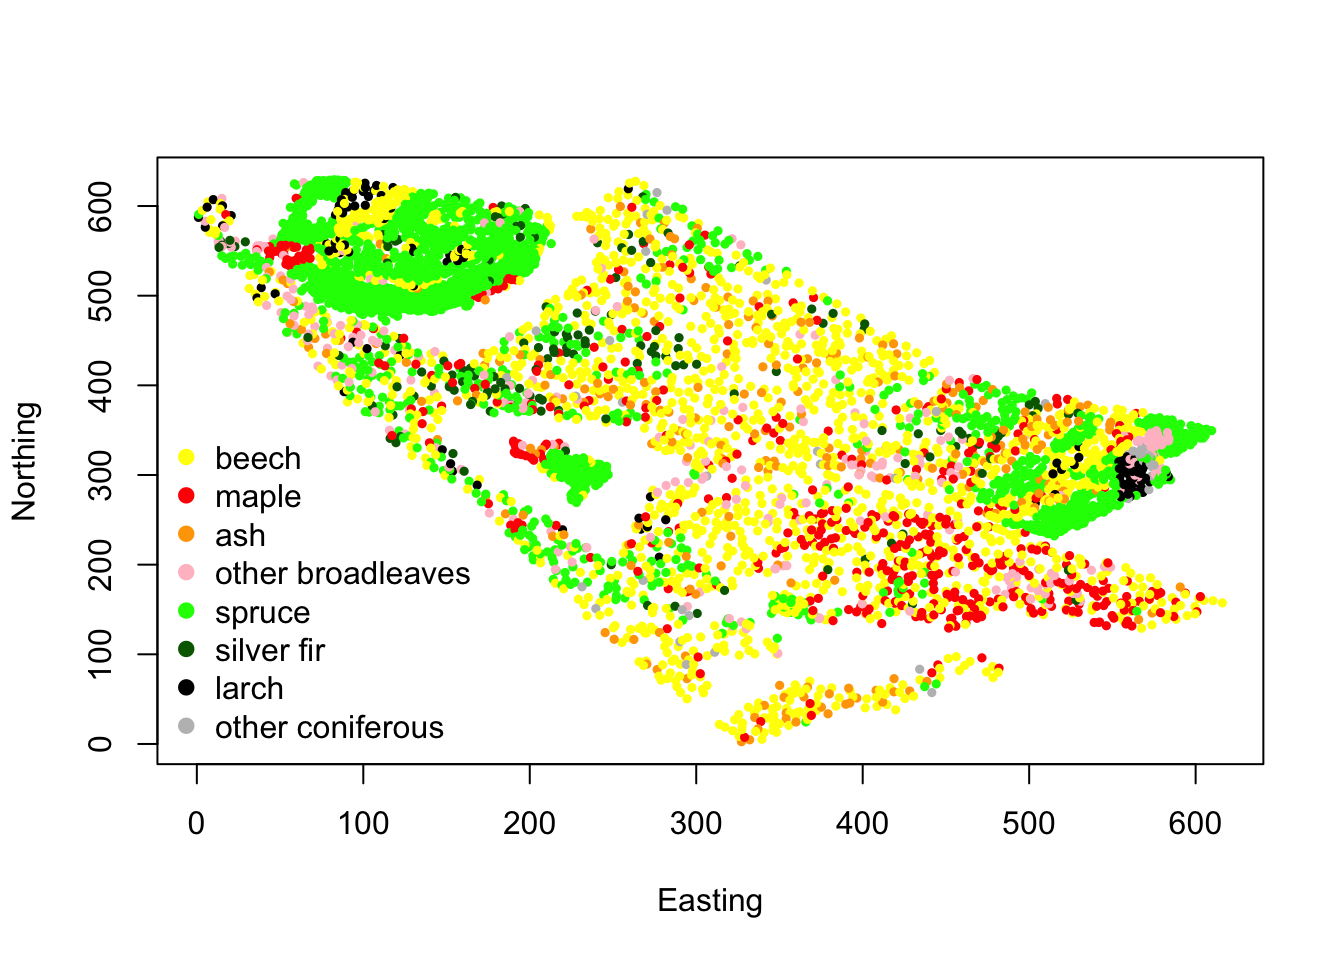
\includegraphics{book_files/figure-latex/unnamed-chunk-87-1} 

}

\caption{Periodic components and their sums.}\label{fig:unnamed-chunk-87}
\end{figure}

\section{스펙트럼이란(spectrum)}\label{spectrum}

\BeginKnitrBlock{theorem}[정상과정의 스펙트럼 표현]
\protect\hypertarget{thm:unnamed-chunk-88}{}{\label{thm:unnamed-chunk-88}
\iffalse (정상과정의 스펙트럼 표현) \fi{} } 어던 정상 시계열이든
근사적으로라도 random superposition of sines and cosines oscillating at
various frequencies로 생각할 수 있다. 즉 자기공분산은 각 주기성분들을
이용해 표현할 수 있으며, 역으로 각 주기성분들도 자기공분산을 이용하여
나타낼 수 있다.
\EndKnitrBlock{theorem}

식 (\eqref{eq:periodrp})의 고정된 진동수 버전 \(\omega_{0}\)를 생각해보자.
\[x_{t}=U_{1}\cos (2\pi\omega_{0}t) + U_{2}\sin(2\pi\omega_{0}t).\]
그리고 \(U_{1}\)과 \(U_{2}\)를 평균이 0이고 분산이 \(\sigma^{2}\)이며
독립인 확률변수들이라고 하자. 위 식에서 한 사이클을 이루기 위해 필요한
시간 길이는 \(1/\omega_{0}\)다. 그러면 자기공분산 \(\gamma(h)\)은 다음과
같이

\begin{eqnarray*}
\gamma(h)&=&\sigma^{2}\cos (2\pi \omega_{0}h)=\frac{\sigma^{2}}{2}e^{-2\pi i \omega_{0}h}+\frac{\sigma^{2}}{2}e^{2\pi i \omega_{0}h}\\
&=&\int_{-1/2}^{1/2}e^{2\pi i \omega h }dF(\omega)
\end{eqnarray*}

리만-스틸체스 적분을 이용해 나타낼 수 있다고 한다. 여기서
\(F(\omega)\)는

\[
F(\omega) 
\begin{cases}
0 & \text{if $\omega < -\omega_{0}$}\\
\sigma^{2}/2 & \text{if $-\omega_{0} \leq \omega < \omega_{0}$}\\
\sigma^{2} & \text{if $\omega \geq \omega_{0}$}
\end{cases}
\] 이다. 여기서 \(F(\omega)\)는 이산확률변수의 누적분포함수처럼
행동하지만, \(F(\infty)=\sigma^{2}=var(x_{t})\neq 1\)이라는 점이 다르다.
비슷한 점에 착안하여 이 \(F(\omega)\)를 \textbf{스펙트럼
분포함수(spectral distribution function)}이라고 부른다.

만약 \(x_{t}\)가 자기공분산 \(\gamma(h)=E[(x_{t+h}-\mu)(x_{t}-\mu)]\)를
갖는 정상과정이라면 단조증가함수 \(F(\omega)\)가 유일하게 존재한다고
한다.

이제 주기성분들의 시계열에 대한 기여도를 나타내는
\textbf{스펙트럼(spectrum)}을 정의해보자. 만약 자기공분산함수
\(\gamma(h)\)가 다음과 같이 절대값의 합이 유한(absolutely summable)
\[\sum_{h=-\infty}^{\infty}|\gamma(h)|<\infty\] 한 확률과정이라고 한다면
다음과 같이
\[\gamma(h)=\int_{-1/2}^{1/2}e^{2\pi i \omega h }f(\omega)d\omega, h=0,\pm 1, \pm 2,\ldots\]
쓸 수 있고 \(\gamma(h)\)의 푸리에 변환(Fourier transform)이 존재하여
(\(f(\omega)\)의 역푸리에 변환)
\[f(\omega)=\sum_{h=-\infty}^{\infty}\gamma(h)e^{-2\pi i \omega h}\] 로
쓸 수 있다. 이 때 \(f(\omega)\)를 \textbf{스펙트럼(spectrum)}이라고
부른다. 이를 이용해 확률과정의 총분산(또는 total power)을 각 진동수별로
분해할 수 있다. 스펙트럼은 자기상관함수의 푸리에 변환이므로
자기상관함수와 일대일 관계에 있으며 다음의 성질을 가지고 있다.

\begin{enumerate}
\def\labelenumi{\arabic{enumi}.}
\item
  \(f(\omega)\geq 0\): 음의 값을 갖지 않는 연속 실수함수
\item
  \(f(\omega)=f(\omega + 2\pi)\): 주기가 \(2\pi\)인 주기함수
  (\(f(\omega)=f(-\omega)\)인 우함수이므로 일반적으로
  \(0\leq \omega \leq \pi\)일 때만 고려한다.)
\item
  \(f(\omega)\)는 확률과정의 \textbf{분산분해(variance
  decomposition)}으로 해석할 수 있으며, \(f(\omega)d\omega\)는
  \((\omega, \omega+d\omega)\)에 속하는 진동수들을 갖는 성분들의 분산에
  대한 기여도를 의미한다. 다시 말해 스펙트럼이 어느 영역의 진동수에서 큰
  값을 갖는다는 것은 해당 진동수들의 분산에 대한 기여도가 크다는 것을
  의미하며, \textbf{이 진동수에 해당되는 주기성분이 시계열의 구성하는 데
  가장 중요한 역할을 한다는 것을 의미한다}.
\item
  스펙트럼과 자기공분산함수는 쌍을 이루어 존재하기 때문에 동일한 정보를
  제공하는 것이며, 어느 통계량이 더 유용한지는 사용하고자 하는 상황에
  따라 다르다고 할 수 있다.
\end{enumerate}

\section{주기가 있는 시계열의 회귀분석(using regression to discover a
periodic
signal)}\label{---using-regression-to-discover-a-periodic-signal}

다음과 같은 모형 \[x_{t}=A\cos (2\pi\omega t + \phi) + w_{t}\] 을
생각해보자. \(\omega=1/50, A=2,\phi=0.6\pi, \sigma_{w}=5\)일 때 모형은
\[x_{t}=2\cos (2\pi t /50 + 0.6 \pi) + w_{t}\] 가 되며 그림으로 출력하면
다음과 같다.

\begin{figure}

{\centering 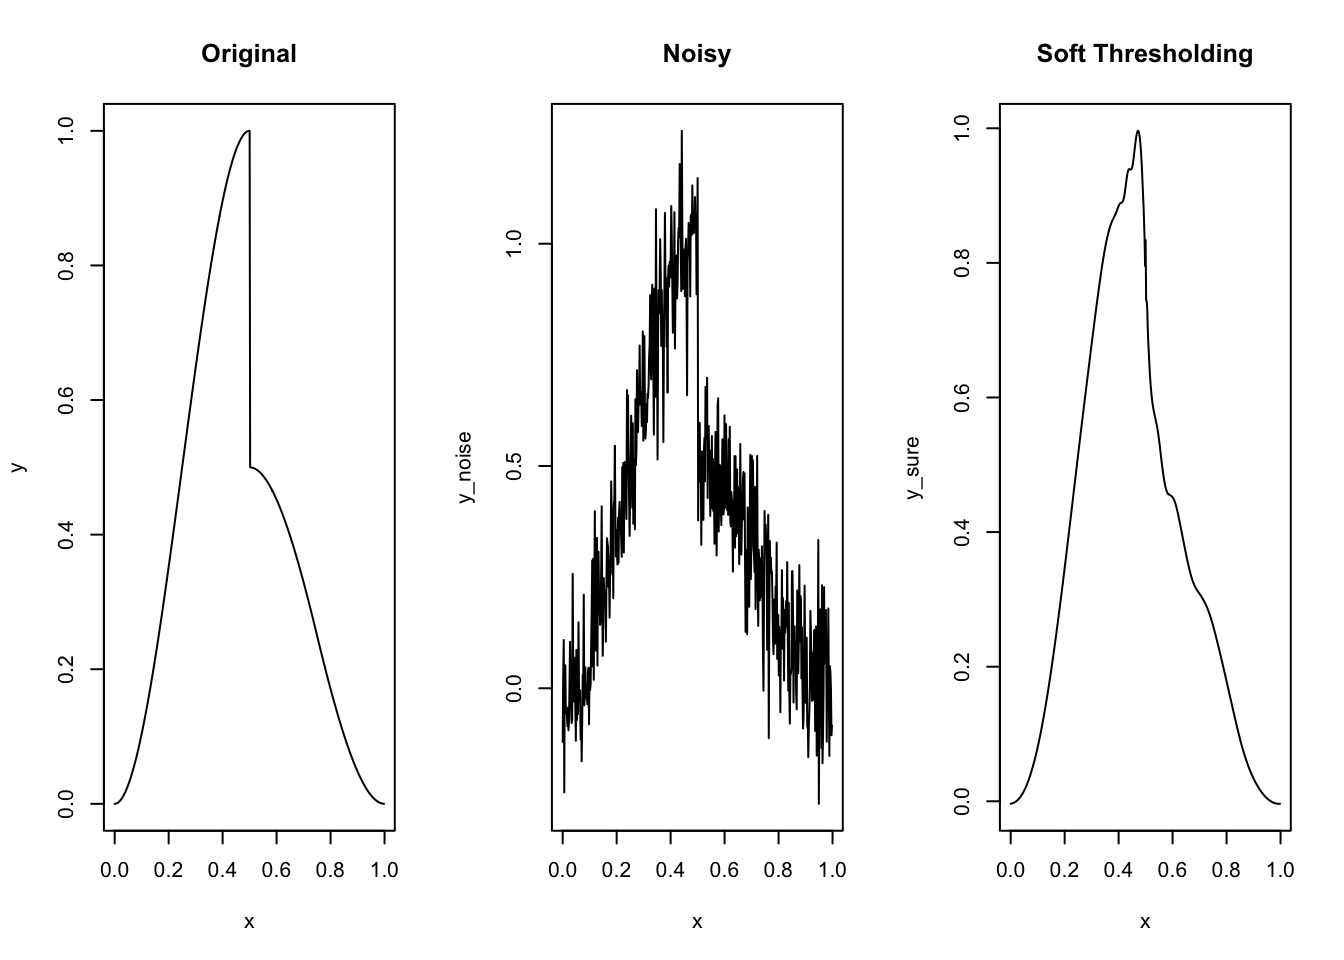
\includegraphics{book_files/figure-latex/unnamed-chunk-89-1} 

}

\caption{Cosine wave with period 50 points (top) with standard Gaussian noise (middle) and with heavy Gaussian noise (bottom).}\label{fig:unnamed-chunk-89}
\end{figure}

진동수 \(\omega=1/50\)이 알려져 있다고 가정하자. 그러나 \(A\)와
\(\phi\)는 모르는 모수라고 가정하자. 삼각함수 공식에 의해
\[A\cos (2\pi \omega t + \phi)=\beta_{1}\cos (2\pi \omega t) + \beta_{2}\sin (2\pi\omega t)\]
이며 \(\beta_{1}=A\cos(\phi), \beta_{2}=-A\sin(\phi)\)이다. 따라서 이
모형은 intercept term을 넣지 않은 일반적인 회귀분석으로 적합할 수 있다.

\section{스펙트럼의 추정(estimation of
spectrum)}\label{-estimation-of-spectrum}

\subsection{푸리에분석(Fourier analysis)}\label{fourier-analysis}

시계열이 관측되었을 때 이들을 진동수에서 정의된 주기성분들로 분해하는
방법을 \textbf{푸리에분석(Fourier analysis)}이라고 한다. 이를 통해 어느
진동수가 중요한 성분이지 따라서 어떤 주기가 시계열에서 중요한 역할을
하는지를 알아낼 수 있다.

\subsection{피리오도그램(periodogram)}\label{periodogram}

스펙트럼을 추정하는 방법을 이해하기 위해서는
\textbf{피리오도그램(periodogram)}에 대한 이해가 필요하다. 이 절의
서술은 \citep{Lim2013}을 참고하였다. 또 다른 참고자료로는
\citep{Shumway2010}이 있다.

다음과 같은 시계열 자료의 수열 \(\{Y_{1}, \ldots, Y_{n}\}\)을 관측한다고
하자. 그러면 \textbf{피리오도그램(periodogram)} \(I_{n}(\omega)\)는
\[I_{n}(\omega)=\frac{1}{n}| \sum_{i=1}^{n}Y_{i}e^{-it\omega}|^{2}\] 로
정의된다. 이 때 \(\omega\in (0,\pi)\)는 \textbf{진동수모수(frequency
parameter)}이다. \(\omega\)가 푸리에
진동수(\(\omega=\frac{2\pi k}{n}, k\in\mathbb{Z}\))일 때 이
피리오도그램은
\[I_{n}(\omega)=\frac{n}{4}\| \tilde{\boldsymbol{\beta}}_{n}(\omega)\|^{2}\]
으로 표현할 수 있다고 한다\citep{Li2008}. 여기서 \(\| \cdot \|\)은
벡터의 \(l_{2}\) 노름이며 \(\tilde{\boldsymbol{\beta}}_{n}(\omega)\)은
최소자승법
\[\tilde{\boldsymbol{\beta}}_{n}(\omega)=\text{arg}\min_{\boldsymbol{\beta}\in\mathbb{R}^{2}}\sum_{i=1}^{n}| Y_{i}-\mathbf{x}_{t}^{T}(\omega)\boldsymbol{\beta}|^{2}\]
의 해다. 그리고 이 때
\(\mathbf{x}_{t}(\omega)=(\cos(\omega t), \sin (\omega t))^{T}\)로
harmonic regressor다.

\section{분위수 피리오도그램(quantile
periodogram)}\label{-quantile-periodogram}

\section{R 예제(R-periodogram)}\label{r-r-periodogram}

여기서는 R에서 피리오도그램을 그리는 방법에 대해 다뤄보겠다.

\begin{enumerate}
\def\labelenumi{\arabic{enumi}.}
\tightlist
\item
  직접 구현
\end{enumerate}

다음 예제는 \citep{Shumway2010}에 있는 scaled periodogram을 구하는
예제이다.

\begin{enumerate}
\def\labelenumi{\arabic{enumi}.}
\setcounter{enumi}{1}
\tightlist
\item
  이미 구현된 패키지 안의 함수들을 이용하는 경우
\end{enumerate}

여기서는 서울특별시 PM10의 1998년 1월부터 2014년 12월까지의 월별 시계열
자료를 이용해 피리오도그램을 그려보겠다.

\begin{Shaded}
\begin{Highlighting}[]
\NormalTok{dataspec <-}\StringTok{ }\KeywordTok{read.csv}\NormalTok{(}\StringTok{'~/Dropbox/Data/PM/MonthlyPMSeoul.csv'}\NormalTok{, }\DataTypeTok{header=}\NormalTok{T)}
\NormalTok{dataspec <-}\StringTok{ }\NormalTok{dataspec[,-}\DecValTok{1}\NormalTok{]}
\NormalTok{dataspec <-}\StringTok{ }\KeywordTok{t}\NormalTok{(dataspec)}
\NormalTok{time_index_month <-}\StringTok{ }\KeywordTok{seq}\NormalTok{(}\DataTypeTok{from =} \KeywordTok{as.POSIXct}\NormalTok{(}\StringTok{"1998-01-01"}\NormalTok{), }\DataTypeTok{to =} \KeywordTok{as.POSIXct}\NormalTok{(}\StringTok{"2014-12-01"}\NormalTok{), }\DataTypeTok{by =} \StringTok{"month"}\NormalTok{)}
\NormalTok{dataspec <-}\StringTok{ }\KeywordTok{xts}\NormalTok{(dataspec[,}\DecValTok{1}\NormalTok{], }\DataTypeTok{order.by=}\NormalTok{time_index_month)}
\KeywordTok{plot}\NormalTok{(dataspec, }\DataTypeTok{type=}\StringTok{'o'}\NormalTok{, }\DataTypeTok{ylim=}\KeywordTok{c}\NormalTok{(}\DecValTok{0}\NormalTok{,}\DecValTok{150}\NormalTok{), }\DataTypeTok{xlab=}\StringTok{"Month"}\NormalTok{, }\DataTypeTok{main=}\StringTok{"Monthly"}\NormalTok{)}
\end{Highlighting}
\end{Shaded}

\begin{figure}

{\centering 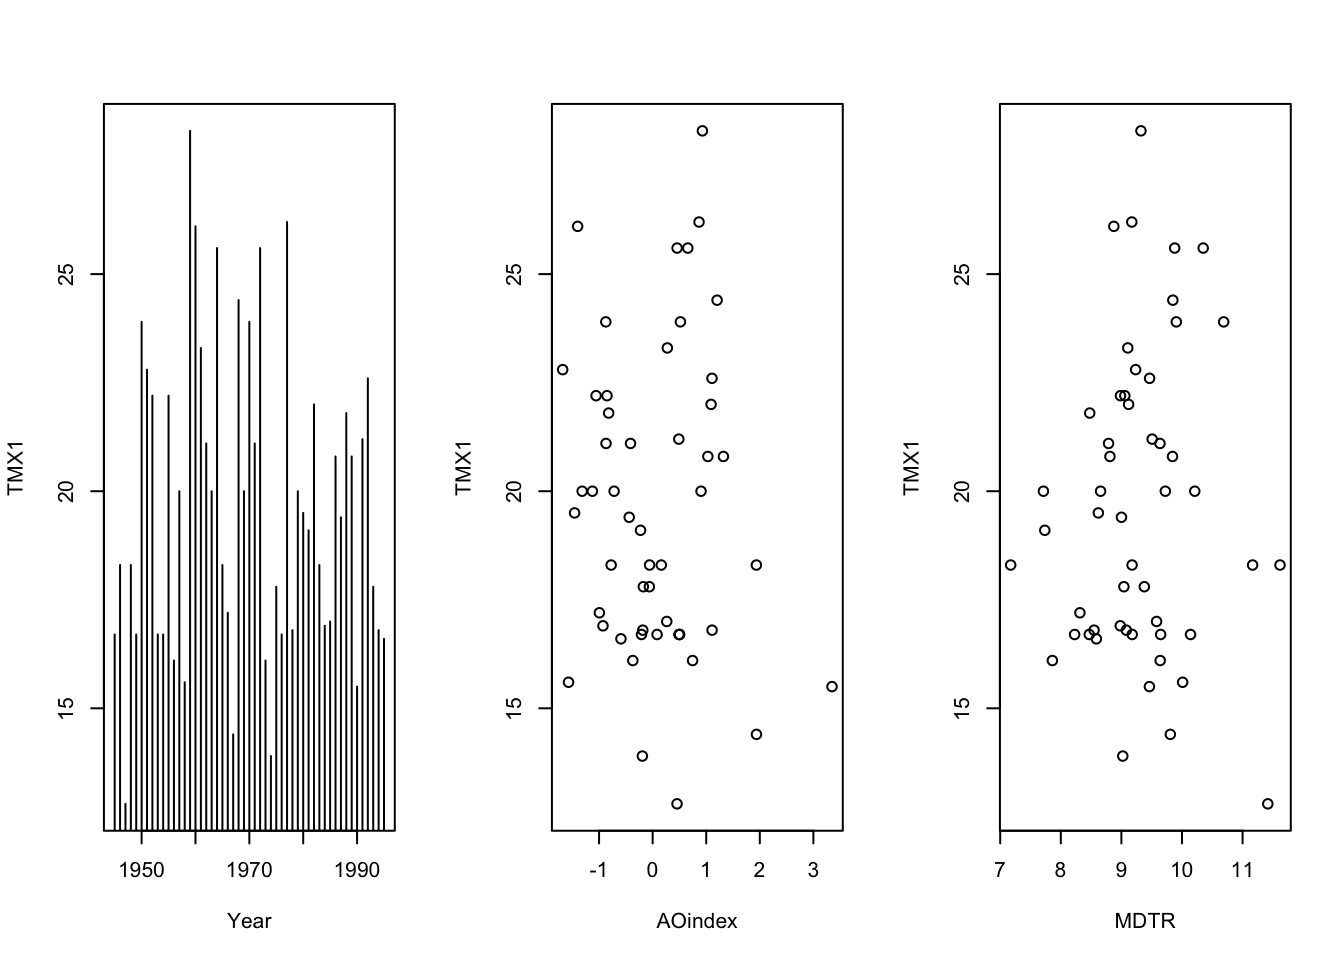
\includegraphics{book_files/figure-latex/unnamed-chunk-90-1} 

}

\caption{Time series of Seoul PM10.}\label{fig:unnamed-chunk-90}
\end{figure}

\texttt{TSA}, \texttt{kza}, \texttt{itsmr} 패키지를 이용한다. 같은
이름의 함수를 사용하기 때문에 실행할 때 주의해야 한다.

\begin{Shaded}
\begin{Highlighting}[]
\NormalTok{TSA::}\KeywordTok{periodogram}\NormalTok{(dataspec, }\DataTypeTok{log=}\StringTok{'yes'}\NormalTok{)}
\end{Highlighting}
\end{Shaded}

\begin{figure}

{\centering 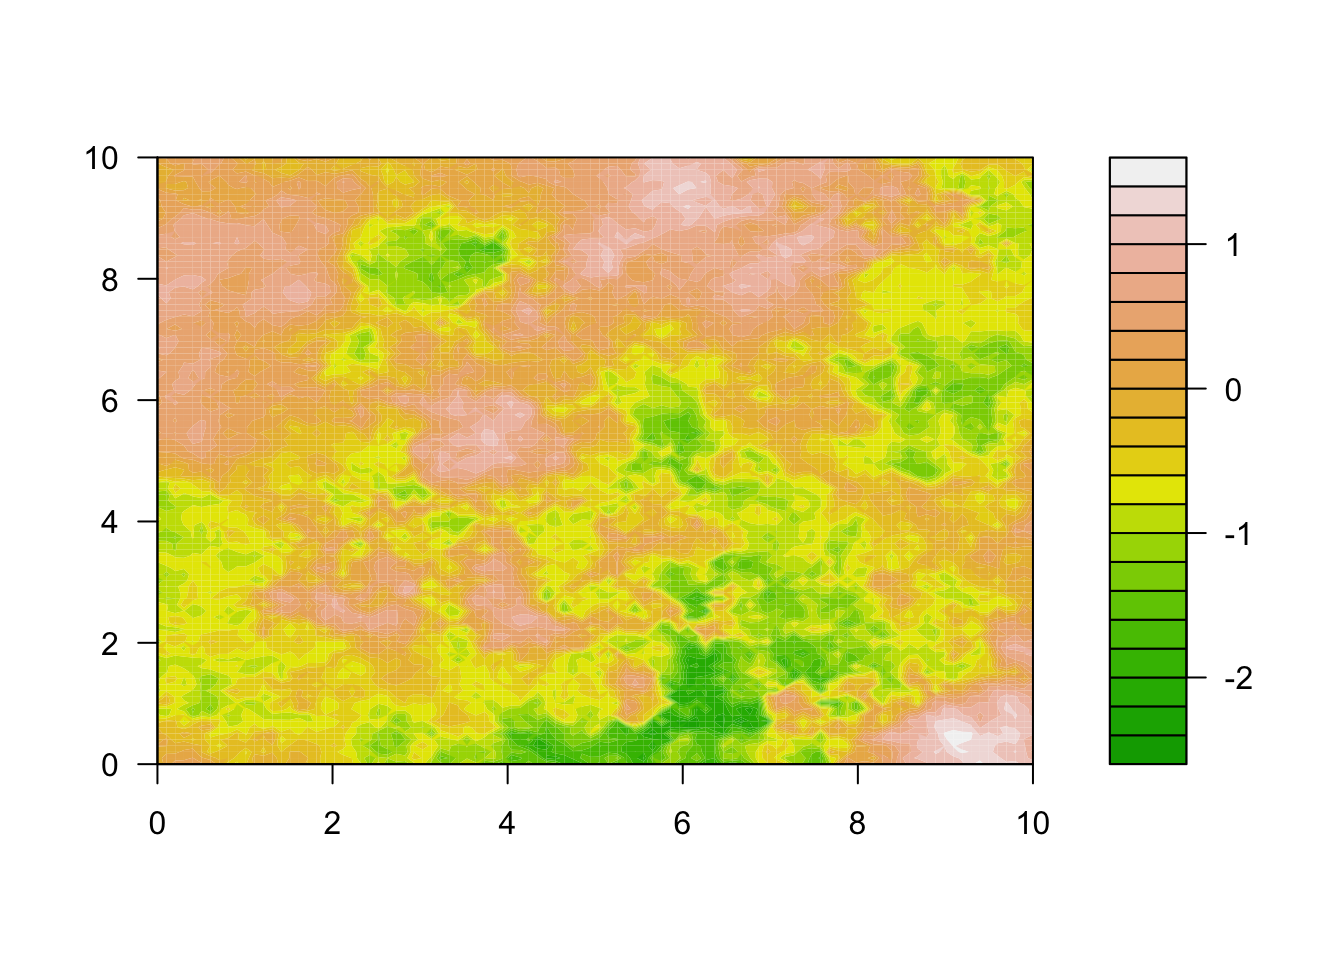
\includegraphics{book_files/figure-latex/unnamed-chunk-91-1} 

}

\caption{Periodogram (using R package TSA).}\label{fig:unnamed-chunk-91}
\end{figure}

\begin{Shaded}
\begin{Highlighting}[]
\KeywordTok{plot}\NormalTok{(kza::}\KeywordTok{periodogram}\NormalTok{(}\KeywordTok{as.numeric}\NormalTok{(dataspec)), }\DataTypeTok{type=}\StringTok{'o'}\NormalTok{)}
\end{Highlighting}
\end{Shaded}

\begin{figure}

{\centering 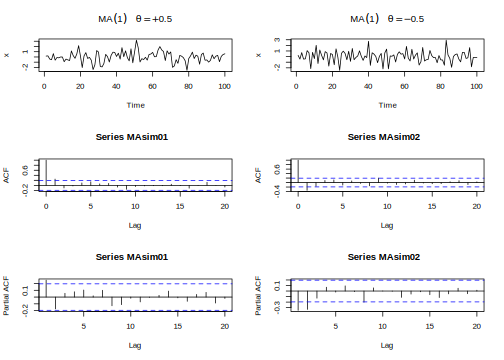
\includegraphics{book_files/figure-latex/unnamed-chunk-92-1} 

}

\caption{Periodogram (using R package kza).}\label{fig:unnamed-chunk-92}
\end{figure}

\begin{Shaded}
\begin{Highlighting}[]
\KeywordTok{plot}\NormalTok{(itsmr::}\KeywordTok{periodogram}\NormalTok{(dataspec))}
\end{Highlighting}
\end{Shaded}

\begin{figure}

{\centering 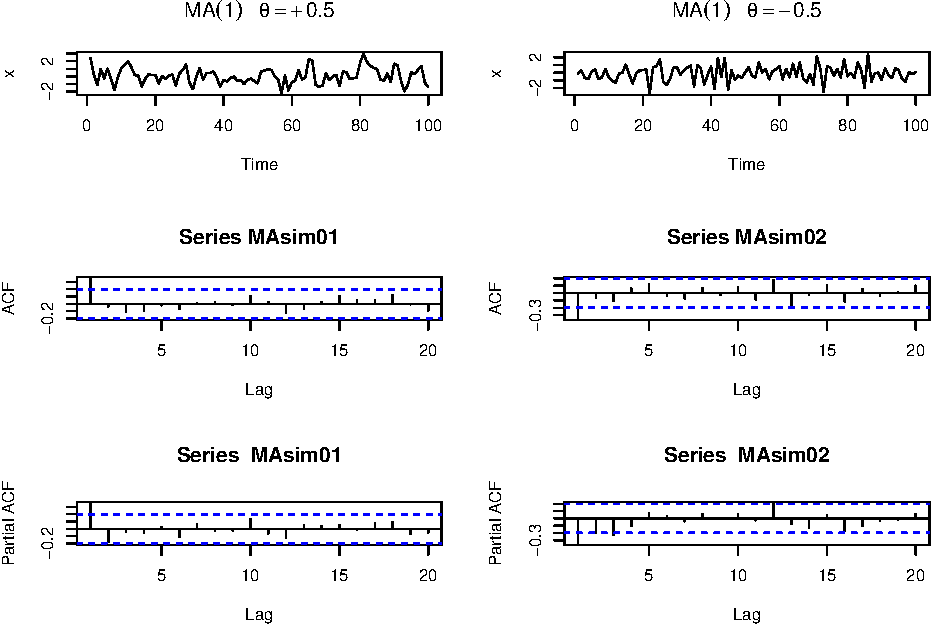
\includegraphics{book_files/figure-latex/unnamed-chunk-93-1} 

}

\caption{Periodogram (using R package itsmr).}\label{fig:unnamed-chunk-931}
\end{figure}\begin{figure}

{\centering 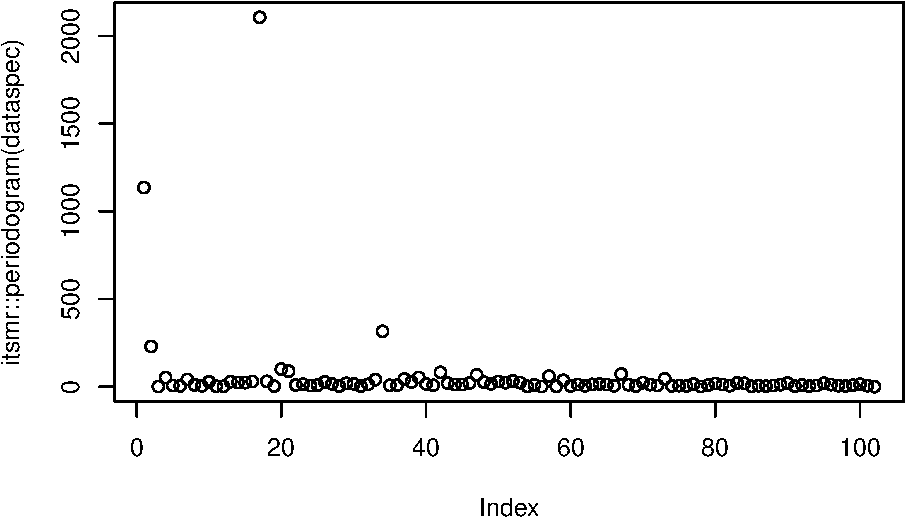
\includegraphics{book_files/figure-latex/unnamed-chunk-93-2} 

}

\caption{Periodogram (using R package itsmr).}\label{fig:unnamed-chunk-932}
\end{figure}

\part{Multiscale Methods in
Statistics}\label{part-multiscale-methods-in-statistics}

\chapter{푸리에로부터 웨이블릿으로}\label{fouriertowavelet}

이 절의 초반부 내용은 \citep{Ogden2012}를 참고하였다.

\section{이산 푸리에변환(discrete Fourier
transform)}\label{-discrete-fourier-transform}

\BeginKnitrBlock{definition}[L2]
\protect\hypertarget{def:unnamed-chunk-94}{}{\label{def:unnamed-chunk-94}
\iffalse (L2) \fi{} }어떤 함수 \(f\)가 \(L^{2}[a,b]\)에 속한다는 것은
\[\int_{a}^{b}f^{2}(x)dx <\infty\] 를 만족할 때이다.
\EndKnitrBlock{definition}

푸리에의 결과는 \(f\in L^{2}[-\pi, \pi]\)인 어떤 함수 \(f\)는 다음과
같이 사인함수와 코사인함수의 무합급수로 표현할 수 있다는 것이다.
\[f(x)=\frac{1}{2}a_{0}+\sum_{j=1}^{\infty}(a_{j}\cos (jx) + b_{j}\sin (jx)),\]
여기서 \(\{ a_{0}, a_{1}, b_{1}, \ldots \}\)들은 계수다.

\BeginKnitrBlock{definition}[직교]
\protect\hypertarget{def:unnamed-chunk-95}{}{\label{def:unnamed-chunk-95}
\iffalse (직교) \fi{} }두 함수 \(f_{1},f_{2}\in L^{2}[a,b]\)는
\(<f_{1},f_{2}=0\)일 때 \textbf{직교(orthogonal)}라고 부른다.
\EndKnitrBlock{definition}

\BeginKnitrBlock{definition}[직교정규]
\protect\hypertarget{def:unnamed-chunk-96}{}{\label{def:unnamed-chunk-96}
\iffalse (직교정규) \fi{} }함수들의 수열 \(\{ f_{j} \}\)는 모든
\(f_{j}\)들이 짝지은 직교(pairwise orthogonal)이며 \(\| f_{j}\|=1\)일 때
\textbf{직교정규(orthonormal)}이라고 한다.
\EndKnitrBlock{definition}

\section{시간주파수해석(time-frequency
analysis)}\label{time-frequency-analysis}

신호를 시간의 관점에서 해석하는 것을 \textbf{시간해석(time
analysis)}라고 한다. 반면에 푸리에해석은 주파수의 관점에서 해석하는
\textbf{주파수해석(frequency analysis)}이다. 우리가 일상생활에서 접하는
신호들은 시간과 주파수를 동시에 고려해야 하는 것들이 많다. 예를 들어,
악보의 각 음표는 어느 시점에 그 음을 발성할 것인지를 나타내는 동시에
어떤 음높이로 발성할 것인지를 나타낸다. 즉 발성할 시점은 시간해석의
관점에서 보는 것이고, 음높이는 주파수해석의 관점에서 보는 것이다.
따라서, 노래라는 신호를 시간해석 또는 주파수해석 각각으로 해석해서는
결코 만족스러운 결과를 얻을 수 없을 것이다. 오늘날 가장 널리 연구되고
사용되는 시간주파수해석법은 웨이블릿의 사용하는 것이다.

\section{웨이블릿(wavelet)}\label{wavelet}

웨이블릿은 뒷장에서도 다시 설명하겠지만, 여기서는 \citep{Shima2016}의
내용을 다룬다.

앞서 보았듯이, 푸리에 변환은 시간 영역에서 진동이 있는 요소들을
추출해낸다는 점에서 효율적인 툴로 알려져있다. 그러나 푸리에 변환은 시간
영역과 주파수 영역을 동시에 보지 못한다는 한계가 있고, 이를 극복하고자
웨이블릿이 등장했다. 웨이블릿 분석의 큰 장점은 신호에 있는 복잡한
정보들을 \textbf{웨이블릿(wavelet)}이라고 하는 기본적인 함수들로
분해(decomposition)할 수 있다는 것이다. 웨이블릿은 localized
waveform으로 시간 및 주파수 스케일의 다양한 범위를 컨트롤할 수 있게
해준다. 또 이 성질은 복구(reconstruction)를 가능하게 해 준다.

푸리에 해석에서의 주파수와는 달리, 웨이블릿 해석에서는
\textbf{척도(scale)}가 중요한 역할을 한다. 척도가 큰 창(window)을 통해서
신호를 관찰하면, 그 신호의 전반적인 특징을 관찰할 수 있다. 즉
웨이블릿이라는 창을 사용해서 신호를 분석하면 신호의 전체적인 모습뿐
아니라 세부적인 모습까지도 분석할 수 있다. 따라서 신호가 가지고 있는
비정상적(nonstationry) 성질들을 나타내는 데 웨이블릿이 유용하다. 예를
들어, 푸리에 해석에서는 신호의 불연속성, 단절(rupture) 등을 잘 식별할 수
없지만 웨이블릿 해석을 사용하면 식별이 가능하다. 이는 웨이블릿이 단순히
신호의 자세한 부분까지를 반영하기 때문이 아니라 신호가 변화하는 부분을
잘 나타내기 때문이다.

\BeginKnitrBlock{definition}[웨이블릿]
\protect\hypertarget{def:unnamed-chunk-97}{}{\label{def:unnamed-chunk-97}
\iffalse (웨이블릿) \fi{} }\textbf{웨이블릿(wavelet)} \(\psi(t)\)는
실변수함수로, localized waveform을 갖으며

\begin{enumerate}
\def\labelenumi{\arabic{enumi}.}
\item
  \(\int_{-\infty}^{\infty}\psi(t)dt=0\)
\item
  \(\int_{-\infty}^{\infty}\psi(t)^{2}dt=1\)
\item
  \(\psi(t)\)의 푸리에 변환 결과인 \(\Psi(t)\)가 \textbf{admissibility
  condition}이라 불리는 다음 성질
  \[C_{\Psi}\equiv\int_{0}^{\infty}\frac{|\Psi(\omega) |^{2}}{\omega}d\omega <\infty\]
  를 만족한다. 이 때 \(C_{\Psi}\)를 \textbf{admissibility constant}라고
  부르며 이 값은 \(\psi(t)\)의 explicit t-dependence에 의존한다고 한다.
\end{enumerate}
\EndKnitrBlock{definition}

\BeginKnitrBlock{example}[Haar 웨이블릿]
\protect\hypertarget{exm:unnamed-chunk-98}{}{\label{exm:unnamed-chunk-98}
\iffalse (Haar 웨이블릿) \fi{} }\textbf{Haar 웨이블릿(Haar wavelet)}은

\begin{equation} 
\psi(t) \equiv
  \begin{cases}
    \frac{1}{\sqrt{2}}       & \quad t\in (0,1],\\
    \frac{-1}{\sqrt{2}}  & \quad t\in (-1,0],\\
    0   & \quad \text{otherwise} \\
  \end{cases}
\end{equation}

으로 정의된다.
\EndKnitrBlock{example}

\begin{figure}

{\centering 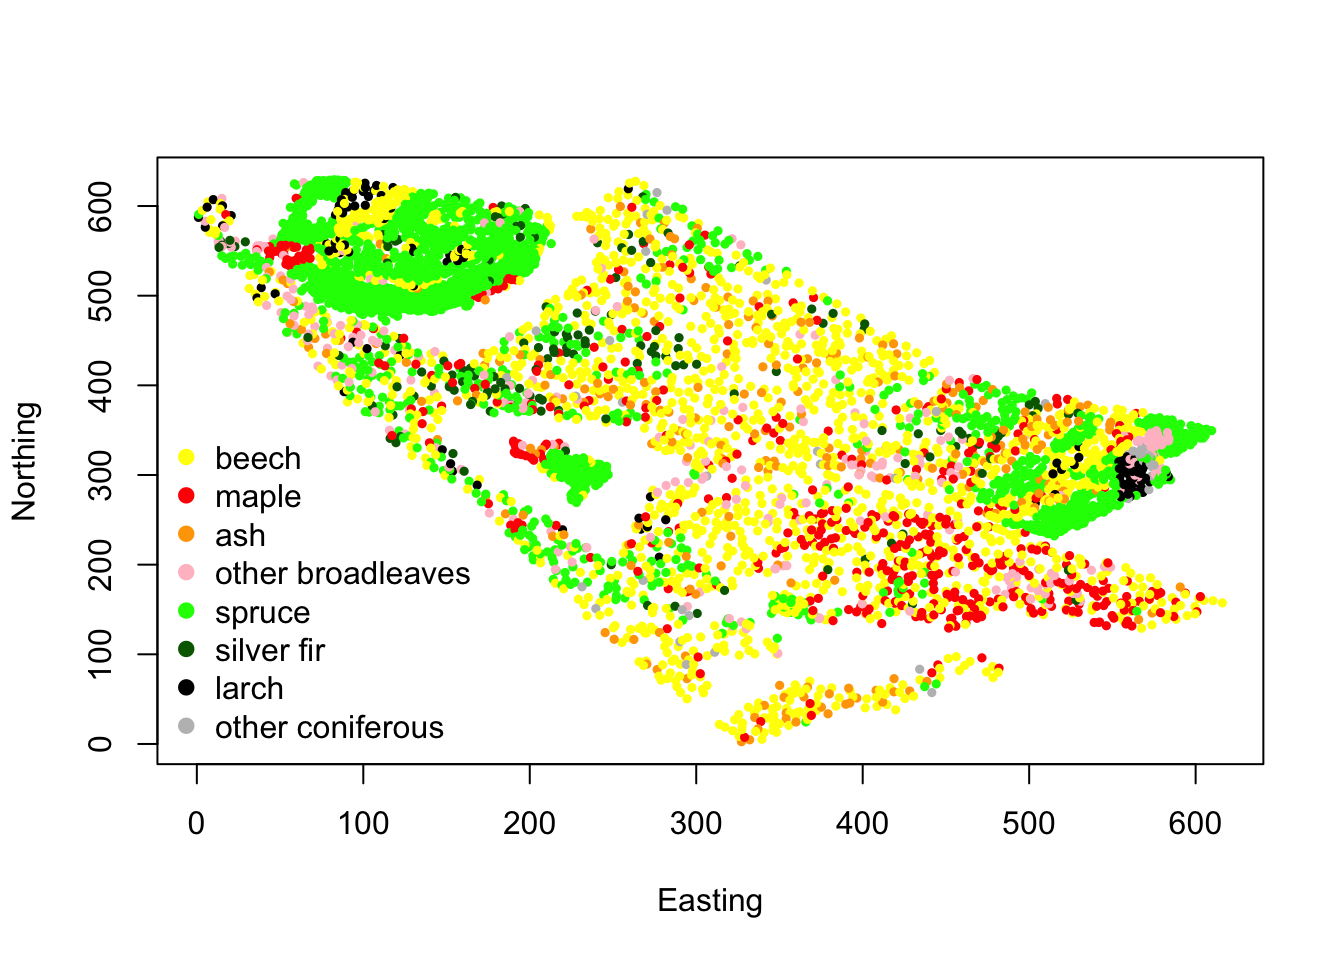
\includegraphics{book_files/figure-latex/unnamed-chunk-99-1} 

}

\caption{Haar wavelet function.}\label{fig:unnamed-chunk-99}
\end{figure}

한 마디로 정리하자면 웨이블릿은 localized oscillating wave라고 볼 수
있다.

\section{웨이블릿 변환(wavelet transform)}\label{-wavelet-transform}

수학적 용어로 \textbf{웨이블릿 변환}은 웨이블릿의
\textbf{합성곱(convolution)}이다. 여기서 잠시 합성곱에 대해 살펴보면,
\(f\), \(g\)라는 두 함수의 \([0,t]\)까지 범위에서 합성곱은
\[\int_{0}^{\tau}f(\tau)g(t-\tau)d\tau\] 이다.

이 합성곲은 웨이블릿의 모양을 변화시키기 위해 두 모수를 갖는다. 하나는
\(a\)로 표시되는 \textbf{팽창모수(dilatation parameter)}이며, domain에서
웨이블릿의 팽창과 수축을 결정해준다. 다른 하나는 \(b\)로 표시되는
\textbf{이동모수(translation parameter)}로, 축을 따라 웨이블릿을
움직여준다.

\begin{figure}

{\centering 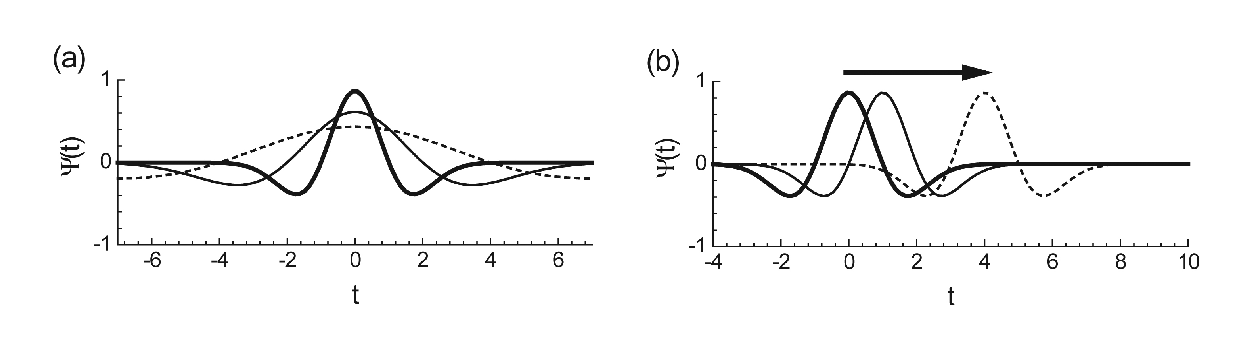
\includegraphics[width=17.5in]{images/multiscale_Transform} 

}

\caption{(a) Dilatation and (b) translation of a wavelet.}\label{fig:unnamed-chunk-100}
\end{figure}

일례로 이동하고 전이된 버전의 Mexican hat wavelet은
\[\psi(\frac{t-b}{a})=[1-(\frac{t-b}{a})^{2}]e^{[-\frac{1}{2}\cdot (\frac{t-b}{a})^{2}]}\]
이 된다. (\(\sigma=1\)인 경우)

\BeginKnitrBlock{definition}[웨이블릿 변환]
\protect\hypertarget{def:unnamed-chunk-101}{}{\label{def:unnamed-chunk-101}
\iffalse (웨이블릿 변환) \fi{} }연속신호 \(x(t)\)의 웨이블릿
\(\psi(t)\)에 대한 \textbf{웨이블릿 변환(wavelet transform)}
\(T(a,b)\)는
\[T(a,b)=w(a)\int_{-\infty}^{\infty}x(t)\psi(\frac{t-b}{a})dt\] 로
정의된다. 여기서 \(w(a)\)는 \textbf{가중치함수(weighted function)}이라고
부른다.

여기서 좀 더 컴팩트한 표현으로
\[\psi_{a,b}(t)=\frac{1}{\sqrt{a}}\psi(\frac{t-b}{a})\] 를 정의해 앞선
식을 \[T(a,b)=\int_{-\infty}^{\infty}x(t)\psi_{a,b}(t)dt\] 로 쓸 수
있다. 앞으로 \(\psi_{a,b}(t)\)을 단순히 \textbf{웨이블릿}으로 부르기로
한다.
\EndKnitrBlock{definition}

일반적으로 \(w(a)=\frac{1}{\sqrt{a}}\)로 정의하는데 그 이유는
\[\int_{-\infty}^{\infty}[\frac{1}{\sqrt(a)}\psi(\frac{t-b}{a})]^{2}dt=\int_{-\infty}^{\infty}\psi(u)^{2}du = 1 \qquad{ \text{ with } u=\frac{t-b}{a}}\]
이기 때문이다.

정리하면 웨이블릿 변환은 time-varying signal에 대한 현미경 역할을 한다.

\section{웨이블릿 공간(wavelet space)}\label{-wavelet-space}

\subsection{다중해상도 분석(multiresolution
analysis)}\label{-multiresolution-analysis}

다중해상도 분석은 사실 함수공간의 집합(a set of function space)이다.
혼란스럽게 용어가 정의되어 있어 주의를 필요로 한다.

\BeginKnitrBlock{definition}[다중해상도 분석]
\protect\hypertarget{def:unnamed-chunk-102}{}{\label{def:unnamed-chunk-102}
\iffalse (다중해상도 분석) \fi{} }\textbf{다중해상도
분석(multiresolution analysis)}란 \(L^{2}(\mathbb{R})\)의 닫힌
부분공간(closed subspace)의 함수공간의 집합
\(\mathcal{V}_{j}:j\in\mathbb{Z}\)으로 \(\mathcal{V}_{j}\)는 다음 조건을
만족한다.

\begin{enumerate}
\def\labelenumi{\arabic{enumi}.}
\item
  \(\cdots \subset \mathcal{V}_{-2} \subset \mathcal{V}_{-1} \subset \mathcal{V}_{0} \subset \mathcal{V}_{1} \subset \mathcal{V}_{2} \ldots \subset L^{2}(\mathbb{R})\)
\item
  \(\bigcap_{j=-\infty}^{\infty}\mathcal{V}_{j}=\{0\}\)
\item
  \(f(t)\in\mathcal{V}_{j}\) if and only if
  \(f(2t)\in\mathcal{V}_{j+1}\) for all integer \(j\)
\item
  집합 \(\{ \phi (t-n), n \in \mathbb{Z}\}\)가 \(\mathcal{V}_{0}\)의
  직교정규기저(orthonormal basis)가 되도록 하는 함수
  \(\phi(t)\in\mathcal{V}_{0}\)이 존재한다.
\end{enumerate}
\EndKnitrBlock{definition}

이 때 \(\phi(t)\)를 \textbf{척도함수(scaling function)} 또는
\textbf{부웨이블릿(father wavelet)}이라고 부른다. 참고할만한 사항으로
다중해상도 분석의 정의는 \(\phi(t)\)의 존재에 대한 어떤 정보도 주지
않는다. 그러나 우리가 만약 바람직한 함수 \(\phi(t)\)를 찾는다면
\(\{ \phi(t-n), n\in\mathbb{Z}\}\)가 span하는 함수공간
\(\mathcal{V}_{0}\)를 정의할 수 있고 앞선 정의의 3번을 이용해
\(V_{j}\)들을 계속해서 만들어내 다중해상도 분석 \(\mathcal{V}_{j}\)를
만들 수 있다. 즉 다시말하면 척도함수 \(\phi(t)\)가 다중해상도 분석
\(\{ \mathcal{V}_{j}\}\)를 생성한다.

\BeginKnitrBlock{definition}[다중해상도 분석의 예]
\protect\hypertarget{def:unnamed-chunk-103}{}{\label{def:unnamed-chunk-103}
\iffalse (다중해상도 분석의 예) \fi{} }\(L^{2}(\mathbb{R})\)에서 어떤
구간 \([2^{-m}n, 2^{-m}(n+1)], \forall n\in\mathbb{Z}\)에서만 상수값을
갖는 모든 함수들의 집합 \(\mathcal{V}_{m}\)을 생각해보자. 그러면
\(\mathcal{V}_{m}\)은 다중해상도 분석의 조건 1부터 3까지를
만족시킨다(\(\phi\)들은 기저이다. 잘 생각해 볼 것)
\EndKnitrBlock{definition}

\begin{figure}

{\centering 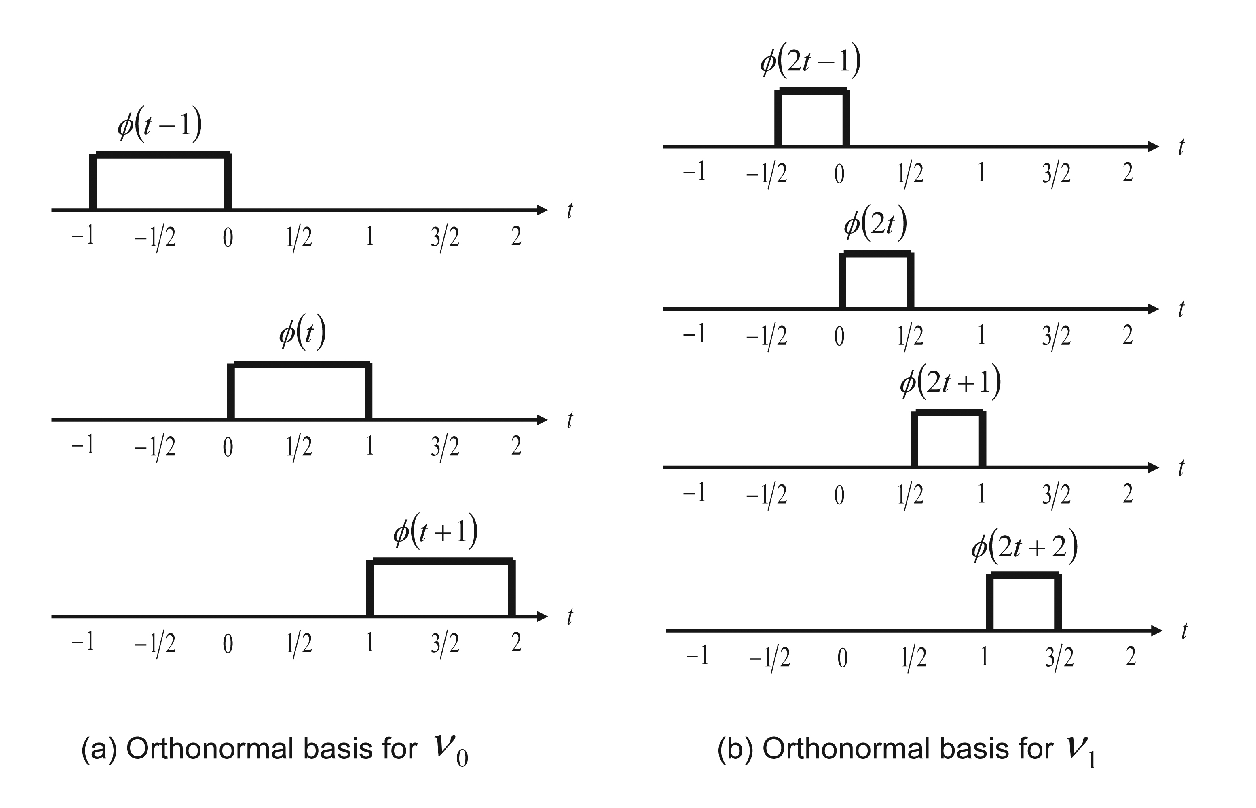
\includegraphics[width=17.44in]{images/multiscale_Multiscaleanalysis} 

}

\caption{(a) Dilatation and (b) translation of a wavelet.}\label{fig:unnamed-chunk-104}
\end{figure}

위 그림에 나오는 \(\{\phi(t-n),n\in\mathbb{Z}\}\)는

\begin{equation} 
\phi(t) \equiv
  \begin{cases}
    1    & \quad 0 \leq t \leq 1\\
    0    & \quad \text{otherwise} \\
  \end{cases}
\end{equation}

로 정의되며 다중해상도분석의 4번 조건을 만족한다. 즉, 어떤 함수
\(f\in\mathcal{V}_{0}\)은
\[f(t)=\sum_{n=-\infty}^{\infty}c_{n}\phi(t-n)\] 으로 표현가능하다.
여기서 \(c_{n}\)은 적절한 상수이다. 따라서 공간 \(\mathcal{V}_{m}\)은
\(\phi(t)\)로 생성되어지는 다중해상도 분석이다.

\subsection{직교분해(orthogonal
decomposition)}\label{orthogonal-decomposition}

다중해상도 분석이 중요한 것은 이것이 \(L^{2}(\mathbb{R})\)에서의
직교정규 기저(orthonormal basis, i.e.~a complete orthonormal set of
functions)를 구성할 수 있게 해준다는 것이다. 이 말을 입증하기 위해 우선
다중해상도 분석 \(\{\mathcal{V}_{j}\}\)가 다음 관계
\[\mathcal{V}_{0}\subset\mathcal{V}_{1}\subset\mathcal{V}_{2}\subset\cdots \subset L^{2}\]
를 만족한다는 것이다.

이제 다음과 같이 \(\mathcal{V}_{0}\)와 \(\mathcal{V}_{1}\)의
\textbf{직교 여공간(orthogonal complement)} \(\mathcal{W}_{0}\)
\[\mathcal{V}_{1}=\mathcal{V}_{0}\oplus\mathcal{W}_{0}\] 을 정의한다.
여기서 \(\oplus\)는 주어진 벡터공간들의 \textbf{직합(direct sum)}이다.
공간 \(\mathcal{W}_{0}\)을 0차원에서의 \textbf{웨이블릿 공간(wavelet
space)}이라고 부른다.

\begin{figure}

{\centering 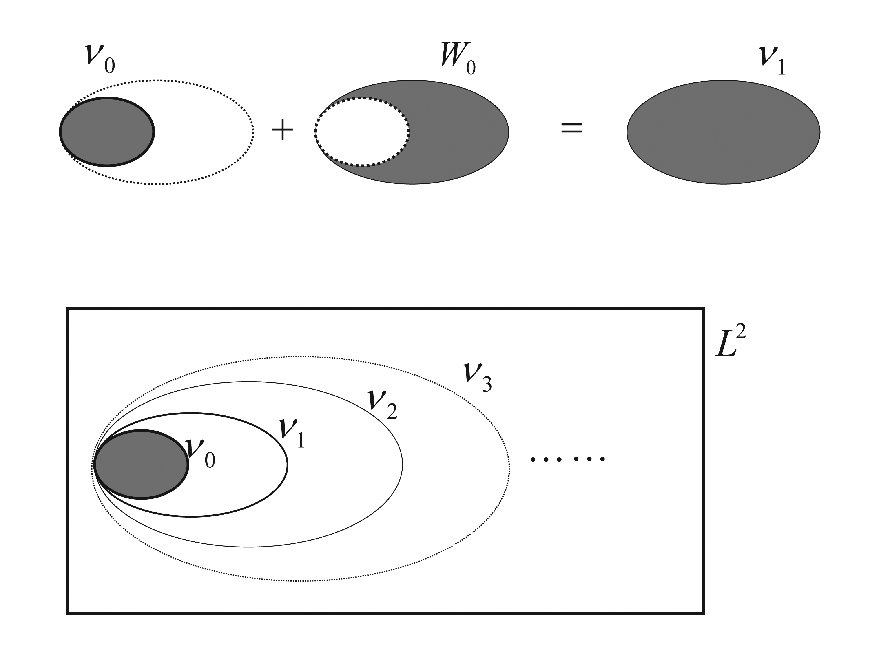
\includegraphics[width=12.17in]{images/multiscale_Orthogonalcomplement} 

}

\caption{Hierarchical structure of the space V and W as subspace of L2.}\label{fig:unnamed-chunk-105}
\end{figure}

위 식은
\[\mathcal{V}_{2}=\mathcal{V}_{1}\oplus\mathcal{W}_{1}=\mathcal{V}_{0}\oplus\mathcal{W}_{0}\oplus\mathcal{W}_{1}\]
으로 확장할 수 있으며, 일반적으로 확장하면
\[L^{2}=\mathcal{V}_{\infty}=\mathcal{V}_{0}\oplus \mathcal{W}_{0} \oplus \mathcal{W}_{1} \oplus \mathcal{W}_{2} \oplus \cdots\]
로 쓸 수 있다. 여기서 \(\mathcal{V}_{0}\)은 함수들의 집합
\(\{ \phi(t-n), n\in\mathbb{Z}\}\)으로 span하는 initial space이다.

최초 공간을 임의로 설정할 수 있기 때문에, 다음과 같이
\[L^{2}=\mathcal{V}_{5}\oplus \mathcal{W}_{5} \oplus \mathcal{W}_{6}\cdots\]
으로 높게 고르거나 또는
\[L^{2}=\mathcal{V}_{-3}\oplus \mathcal{W}_{-3} \oplus \mathcal{W}_{-2}\cdots\]
와 같이 낮은 해상도를 고를 수도 있다. 극단적으로는
\[L^{2}=\cdots\oplus \mathcal{W}_{-1} \oplus \mathcal{W}_{0} \oplus \mathcal{W}_{1}\cdots\]
로 \(-\infty\)를 취하기도 한다. 이와 같은 표현을 \(L^{2}\)에서의
\textbf{직교분해(orthogonal decomposition)}으로 부른다. 이것은 즉 어떤
함수 \(x\in L^{2}(\mathbb{R})\)은 다음과 같이
\[x(t)=\cdots + g_{-1}(t)+g_{0}(t)+g_{1}(t)+\cdots .\]
\(g_{j}\in\mathcal{W}_{j}\)의 무한합으로 분해할 수 있다.

\subsection{직교정규 기저 구성(orthonormal basis
construction)}\label{--orthonormal-basis-construction}

웨이블릿 공간 \(\{ W_{j} \}\)들의 직교 성질에 대해 좀 더 자세히
살펴보자. 앞선 직합으로 표시된 식들에 의해
\[\mathcal{W}_{0}\subset \mathcal{V}_{1} \text{ and } \mathcal{W}_{1} \subset \mathcal{V}_{2}\]
관계를 갖는다. 다중해상도 분석 \(\{\mathcal{V}_{j}\}\)의 정의의 관점에서
봤을 때,
\[f(t)\in \mathcal{V}_{1} \Longleftrightarrow f(2t)\in \mathcal{V}_{2}\]
이고 그러므로
\[f(t)\in \mathcal{W}_{0} \Longleftrightarrow f(2t)\in \mathcal{W}_{1}\]
이다. 더 나아가서, 다중해상도 분석의 4번 조건은
\[f(t)\in \mathcal{W}_{0} \Longleftrightarrow f(t-n)\in\mathcal{W}_{0} \text{ for any } n\in\mathbb{Z}\]
가 되게 만든다.

이제 위 사실들을 가지고 \(L^{2}(\mathbb{R})\)에서의 직교정규 기저들을
만들어보자. 우선 \(\mathcal{W}_{0}\)에서 직교정규 기저
\(\{\psi(t-n),n\in\mathbb{Z}\}\)를 만드는 함수\(\psi(t)\)가 있다고 하자.
그러면 다음과 같은 표기
\[\phi_{0,n}(t)\equiv\psi(t-n)\in\mathcal{W}_{0]}\] 를 이용해 이것의
scaled version을 \[\phi_{1,n}(t)=\sqrt{2}\psi(2t-n)\] 으로 정의하고
이것은 \(\mathcal{W}_{1}\)의 직교정규 기저가 된다. \(\sqrt{2}\)는 정규
조건을 유지하기 위해 들어간 상수다.
\[\int_{-\infty}^{\infty}\psi_{0,n}(t)^{2}dt=\int_{-\infty}^{\infty}\psi_{1,n}(t)^{2}dt=1.\]

같은 과정들을 반복하면 \[\psi_{m,n}(t)=2^{m/2}\psi(2^{m}t-n)\] 이라는
관계식을 얻을 수 있으며 이 때 \(\psi_{m,n}\)은 \(\mathcal{W}_{m}\)의
직교기저가 된다. 이러한 결과물들을 앞선 함수
\(x\in L^{2}(\mathbb{R})\)의 직교분해 식에 넣을 경우

\begin{eqnarray*}
x(t)&=& \cdots + g_{-1}(t)+g_{0}(t)+g_{1}(t)+\cdots\\
&=&\cdots + \sum_{n=-\infty}^{\infty}c_{-1,n}\psi_{-1,n}(t)+\sum_{n=-\infty}^{\infty}c_{0,n}\psi_{0,n}(t) + \sum_{n=-\infty}^{\infty}c_{1,n}\psi_{1,n}(t)+\cdots \\
&=&\sum_{m=-\infty}^{\infty}\sum_{n=-\infty}^{\infty}c_{m,n}\psi_{m,n}(t).
\end{eqnarray*}

결과적으로 family \(\psi_{m,n}(t)\)가 \(L^{2}(\mathbb{R})\)의 직교정규
기저가 된다. 위 결과를 다음 정리로 요약할 수 있다.

\BeginKnitrBlock{theorem}[직교정규 기저의 구성]
\protect\hypertarget{thm:unnamed-chunk-106}{}{\label{thm:unnamed-chunk-106}
\iffalse (직교정규 기저의 구성) \fi{} }\(\{ \mathcal{V}_{j}\}\)를
다중해상도 분석이라고 하고 공간 \(\mathcal{W}_{0}\)를
\(\mathcal{W}_{0}=\mathcal{V}_{1}/\mathcal{V}_{0}\)으로 정의한다. 만약
어떤 함수 \(\psi(t)\)가 \(\mathcal{W}_{0}\)의 정규직교 기저
\(\{ \psi(t-n),n\in\mathbb{Z}\}\)를 만들어 낸다면, 함수들의 집합
\(\{\psi_{m,n},m,n\in\mathbb{Z}\}\)는
\[\psi_{m,n}(t)=2^{m/2}\psi(2^{m}t-n)\] \(L^2{\mathbb{R}}\)에서의
직교정규 기저를 구성한다.
\EndKnitrBlock{theorem}

여기서 소개된 \(\psi(t)\)는 웨이블릿을 결정하는 데, 즉 Haar wavelet이냐
mexican hat wavelet이냐 등을 결정하는 데 쓰이므로, \(\mathcal{W}_{m}\)을
\textbf{웨이블릿 공간(wavelet space)}이라고 부르며 함수 \(\psi(t)\)를
\textbf{모웨이블릿(mother wavelet)}이라고 부른다.

\subsection{두-스케일 관계(two-scale
relation)}\label{--two-scale-relation}

앞서 언급한 내용들은 \(L^{2}(\mathbb{R})\)에서의 직교정규 기저
\(\{\psi_{m,n} \}\)을 모웨이블릿 \(\psi(t)\)의 명시적 함수 형태를
특정지음으로써 구성할 수 있다는 것을 암시한다. 그럼 이제 남아있는 일은
모웨이블릿 \(\psi(t)\)를 이용해 다중해상도 분석이 주어졌을 때
\(\mathcal{W}_{0}=\mathcal{V}_{1}/\mathcal{V}_{0}\)이 포함된 공간에서
정규직교 기저 \(\{ \psi(t-n), n\in\mathbb{Z}\}\)를 이끌어내는 일이다.
우리는 \(\psi(t)\)를 척도함수 \(\phi(t)\)를 잘 살펴봄으로써 찾아낼 수
있었음을 상기해야 한다.

다음에는 주어진 다중해상도 분석에서 모웨이블릿 \(\psi(t)\)를 구성하기
위한 척도함수의 중요한 특징인 \textbf{두-스케일 관계(two-scale
relation)}에 대해 언급하겠다. 우리는 \(\mathcal{V}_{m}\)에 있는 모든
함수들이 \(\mathcal{V}_{0}\)에 있는 것들에서 \(2^{m}\)만큼 스케일링하여
얻을 수 있다는 걸 안다. 이 결과를 스케일링 함수에 적용시키면
\[\phi_{0,n}(t)\equiv \phi(t-n) \in \mathcal{V}_{0}\] 이고 이것은
\[\phi_{m,n}(t)=2^{m/2}\phi(2^{m}t-n), m\in\mathbb{Z}\] 가
\(\mathcal{V}_{m}\)의 직교정규 기저가 되는 것으로 이어진다. 특히
\(\phi \in \mathcal{V}_{0}\subset \mathcal{V}_{1}\)이고
\(\phi_{1,n}(t)=\sqrt{2}\phi(2t-n)\)이 \(\mathcal{V}_{1}\)의 직교정규
기저이기 때문에, \(\phi(t)\)는 \(\phi_{1,n}(t)\)에 의해 확장되어질 수
있다. 이것은 다음 정리로 요약할 수 있다.

\BeginKnitrBlock{theorem}[두-스케일 관계]
\protect\hypertarget{thm:unnamed-chunk-107}{}{\label{thm:unnamed-chunk-107}
\iffalse (두-스케일 관계) \fi{} }척도함수 \(\phi(t)\)가 다중척도 해석
\(\{ \mathcal{V}_{j}\}\)을 생성할 때, 다음과 같은 관계식을 얻을 수 있다.
\[\phi(t)=\sum-{n=-\infty}^{\infty}p_{n}\phi_{1,n}(t)=\sqrt{2}\sum_{n=-\infty}^{\infty}p_{n}\phi(2t-n),\]
이 때 \[p_{n}=\int_{-\infty}^{\infty}\phi(t)\phi_{1,n}(t)dt\] 이다. 이
식을 \(\phi(t)\)의 \textbf{두-스케일 관계(two-scale relation)}식이라고
부른다. 그리고 계수 \(p_{n}\)을 \textbf{척도함수계수(scaling function
coefficients)}라고 부른다.
\EndKnitrBlock{theorem}

\BeginKnitrBlock{example}[두-스케일 관계의 예]
\protect\hypertarget{exm:unnamed-chunk-108}{}{\label{exm:unnamed-chunk-108}
\iffalse (두-스케일 관계의 예) \fi{} }다음과 같이
\(L^{2}(\mathbb{R})\)의 함수들을 모두 포함하고 구간
\([2^{-m}n, 2^{-m}(n+1)], n\in\mathbb{Z}\)에서 상수값을 갖는 공간
\(\mathcal{V}_{m}\)에 대해 생각해보자. 이 다중해상도 해석은 앞 예제에서
등장했던 척도함수 \(\phi(t)\)에 의해 생성됨이 알려져있다.
\[p_{0}=p_{1}=\frac{1}{2} \text{ and } p_{n}=0 \text{ for }n\neq 0,1.\]
따라서, 이 예의 두-스케일 관계식은 \[phi(t)=\phi(2t)+\phi(2t-1)\] 이
된다.
\EndKnitrBlock{example}

\begin{figure}

{\centering 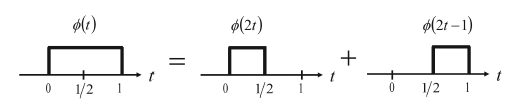
\includegraphics[width=7.33in]{images/multiscale_Twoscale} 

}

\caption{Two-scale relation of phi(t).}\label{fig:unnamed-chunk-109}
\end{figure}

\subsection{모웨이블릿(mother wavelet)}\label{mother-wavelet}

이제 \(L^{2}(\mathbb{R})\)에서 직교정규 기저를 만들 수 있도록 하는
모웨이블릿 \(\psi(t)\)를 결정할 차례다. 모웨이블릿
\(psi(t)=\psi_{0,0,}(t)\in\mathcal{W}_{0}\)가 \(\mathcal{V}_{1}\)에 의해
spanned되어짐을 상기하자. 즉
\(\mathcal{W}_{0}\subset \mathcal{V}_{1}\)이다. 정리하면, \(\psi(t)\)는
\(\phi(2t)\)들의 가중합으로 표현할 수 있다.
\[\psi(t)=\sum_{n=-\infty}^{\infty}q_{n}\sqrt{2}\phi(2t-n), n\in\mathbb{Z}.\]
이 때 계수 \(q_{n}\)은 \textbf{웨이블릿 계수(wavelet coefficients)}라고
불리며 \[q_{n}=(-1)^{n-1}p_{-n-1}\] 로 주어진다.

\BeginKnitrBlock{theorem}[모웨이블릿]
\protect\hypertarget{thm:unnamed-chunk-110}{}{\label{thm:unnamed-chunk-110}
\iffalse (모웨이블릿) \fi{} } 만약 \(\{ \mathcal{V}_{m}\}\)이 척도함수
\(\phi(t)\)를 갖는 다중해상도 해석이라고 한다면, 모웨이블릿
\(\psi(t)\)는
\[\psi(t)=\sqrt{2}\sum_{n=-\infty}^{\infty}(-1)^{n-1}p_{-n-1}\phi(2t-n), n\in\mathbb{Z}\]
로 주어진다. 이 때 \(p_{n}\)은 척도함수 \(phi(t)\)의 계수이다. 그리고 이
\(p_{n}\)은 유일하게 정해진다.
\EndKnitrBlock{theorem}

즉 위 정리에 의하면 모웨이블릿 \(\psi(t)\)는 주어진 다중해상도 해석에서
척도함수 \(\phi(t)\)를 특정화하면 얻을 수 있다.

\subsection{다중해상도 표현(multiresolution
representation)}\label{-multiresolution-representation}

앞서 했던 내용들을 종합하면, \(L^{2}(\mathbb{R})\)을 span하는 척도함수들
\(\phi_{j,k}(t)\)와 웨이블릿들 \(\psi_{j,k}(t)\)의 직교정규 기저를 얻을
수 있었다.
\[L^{2}=\mathcal{V}_{j_{0}}\oplus\mathcal{W}_{j_{0}}\oplus\mathcal{W}_{j_{0}+1}\oplus\cdots,\]
이 식을 이용해, 어떤 함수 \(x(t)\in L^{2}(\mathbb{R})\)은
\[x(t)=\sum_{k=-\infty}^{\infty}S_{j_{0},k}\phi_{j_{0},k}(t)+\sum_{k=-\infty}^{\infty}\sum_{j=j_{0}}^{\infty}T_{j,k}\psi_{j,k}(t)\]
로 확장해 표현할 수 있다. 이 때, 최초의 척도 \(j_{0}\)은 0 또는 다른
정수 또는 어떤 척도함수를 쓰지 않을때에는 \(-\infty\)까지 될 수도 있다.
계수 \(T_{j,k}\)는 이산 웨이블릿 변환이 이미 주어졌을때 identified
되어진다. 종종 \(T_{j,k}\)를 \textbf{웨이블릿 계수(wavelet
coefficient)}라고 부르며, 대응되는 \(S_{j,k}\)를
\textbf{근사계수(approximation coefficient)}라고 부른다.

앞의 식을 좀 더 단순화하기 위해
\[x_{j_{0}}(t)=\sum_{k=-\infty}^{\infty}S_{j_{0},k}\phi_{j_{0},k}(t)\]
신호 \(x(t)\)의 척도 \(j_{0}\)에 대한 \textbf{연속 근사(continous
approximation)}을 생각하자. 연속 근사를 보면
\(j_{0}\rightarrow \infty\)일 때 \(x_{j_{0}}(t)\rightarrow x(t)\)가
된다. (왜냐면 \(L^{2}=\mathcal{V}_{\infty}\)이기 때문이다)

더불어, 다음과 같이
\[z_{j}(t)=\sum_{k=-\infty}^{\infty}T_{j,k}\psi_{j,k}(t)\] 라는 표기를
도입한다. 이 때 \(z_{j}(t)\)는 척도 \(j\)에서의 \textbf{신호 상세(signal
detail)}라고 부른다. 그러면 다중해상도 표현은
\[x(t)=x_{j_{0}}(t)+\sum_{j=j_{0}}^{\infty}z_{j}(t)\] 가 된다. 이 표현은
원래 신호 \(x(t)\)를 이것의 연속 근사인 임의의 척도 색인 \(j_{0}\)에서의
\(x_{j_{0}}\)와 척도 \(j_{0}\)에서 무한대까지의 신호 상세를 더한 값으로
내타낼 수 있다다.

또한 \(\mathcal{V}_{j+1}=\mathcal{V}_{j}\oplus\mathcal{W}_{j}\)를 이용해
\[x_{j+1}(t)=x_{j}(t)+z_{j}(t)\] 로 쓸 수 있다. 이것은 우리가 어떤 척도
\(j\)에서의 연속 근사 신호에 신호 상세를 더하면 더 작은 척도
\(j+1\)에서의 연속 근사식을 얻을 수 있다는 것이다. 이 식을
\textbf{다중해상도 표현(multiresolution representation)}이라고 부른다.

\chapter{다중척도 방법론}\label{multiscale}

이 장에서는 통계학에서의 다중척도 방법론을 다룬다. 주된 내용은 2015년
지도교수님의 특강 수업 내용이다. 이 문서에 담겨있는 그림들은
\citep{Nason2010}을 참고하였다.

\section{다중척도 변환(multiscale
transform)}\label{-multiscale-transform}

다음과 같은 형태의 벡터 자료를 생각해보자.
\[ \mathbf{y}=(y_{1},\ldots,y_{n}), n=2^{J}\] 여기서 \(n=2^{J}\)는
굉장히 강하고 불편한 조건이다. 예를 들어, 자료의 길이가 800개 또는 900개
정도라면 자료의 길이가 2의 배수라는 조건에 맞게 데이터를 일부를 버려야
한다. 또한 \(\mathbf{y}\)는 등간격 자료(equally spaced data)여야 한다.
예를 들어, 시계열 자료의 경우 오늘 10시, 내일 10시에 관측된 값이 자료에
있으면 그 다음 값은 모레 10시에 관측된 값이여야 하며, 11시에 관측된 값이
와서는 안 된다는 것이다.

다중척도 방법론에서 알고 싶어하는 가장 중요한 정보는 각기 다른
\textbf{척도(scale)}와 \textbf{위치(location)}에서의 \(\mathbf{y}\)의
\textbf{상세(detail)}이다. 여기서 척도는 수준(level), 해상도(resolution)
등으로 불리기도 하며 통계학 용어로 번역하자면 분산, 파워(power),
도수(frequency) 등으로 말할 수 있다. 장소라는 것은 관측값을 관찰한
정의역(domain)을 의미하며, 시간 자료면 시간, 공간 자료면 공간이
로케이션이 된다. 한편 상세의 정의는 다음과 같다.

\BeginKnitrBlock{definition}[상세]
\protect\hypertarget{def:unnamed-chunk-111}{}{\label{def:unnamed-chunk-111}
\iffalse (상세) \fi{} }주어진 자료 \(\mathbf{y}\)의
\textbf{상세(detail)} \(d_{k}\)는

\begin{equation}
d_{k}=y_{2k}-y_{2k-1},\qquad{k=1,2,\ldots,\frac{n}{2}}
\end{equation}

이다.
\EndKnitrBlock{definition}

\BeginKnitrBlock{example}[상세의 계산]
\protect\hypertarget{exm:unnamed-chunk-112}{}{\label{exm:unnamed-chunk-112}
\iffalse (상세의 계산) \fi{} }다음과 같이 길이 8인 자료
\(\mathbf{y}=(y_{1},y_{2},\ldots,y_{8})\)가 있다고 하자. 그러면 이
자료의 상세는

\begin{equation}
d_{1}=y_{2}-y_{1}, d_{2}=y_{4}-y_{3}, d_{3}=y_{6}-y_{5}, d_{4}=y_{8}-y_{7}
\end{equation}

와 같이 4개가 존재한다. 여기서 특이한 점은 \(y_{3}-y_{2}\)와 같은 값들은
고려하지 않는다는 것이다. 이는 어떻게 관측하느냐에 따라 \(d_{k}\)가
완전히 달라질 수도 있다는 말이다. 즉 상세는 평행 이동 불변(translation
invariant)하지 않다.
\EndKnitrBlock{example}

한편, 상세와 유사한 개념으로 \textbf{성김(coarser)}을 정의한다.

\BeginKnitrBlock{definition}[성김]
\protect\hypertarget{def:waveletcoarser}{}{\label{def:waveletcoarser}
\iffalse (성김) \fi{} }주어진 자료 \(\mathbf{y}\)의
\textbf{성김(coarser)} \(c_{k}\)은

\begin{equation}
c_{k}=y_{2k}+y_{2k-1},\qquad{k=1,2,\ldots,\frac{n}{2}}
\end{equation}

이다.
\EndKnitrBlock{definition}

성김은 \textbf{매끄러움(smooth)}으로 불리기도 하며, +의 개념이다. 상세는
\textbf{차이(difference)}로 불리기도 하며, -의 개념이다. \(c_{k}\)와
\(d_{k}\)를 알고 있으면 원래 자료들의 원소 \(y_{i}\)들도 다 알아낼 수
있다. 이렇게 다중척도 변환은 원래 신호를 재구성(reconstruction)할 수
있어야 한다.

한편, 앞선 예제에서처럼 자료의 길이가 8일 때, (특정 수준에서) 얻을 수
있는 최대 상세는 4개이다. 이것을 \textbf{가장 섬세한
상세(finest-detail)}라고 한다. 그런데 우리가 \(c_{k}\)를 이용해서
\(d_{k}(=d_{J-1})\)보다 좀 더 엉성한 상세를 얻고 싶을 수 있다. 그러면 그
것보다 낮은 수준, 즉 \(J-2\) 수준을 생각하면 된다. \(J-2\) 수준에서의
상세는

\begin{eqnarray}
d_{J-2,l}&=&c_{J-1,2l}-c_{J-1,2l-1},l=1,2,\ldots,\frac{n}{4}\nonumber\\
&=&(y_{4l}+y_{4l-1})-(y_{4l-2}+y_{4l-3})
\end{eqnarray}

로 정의된다. 예를 들어, \(d_{J-2,1}=(y_{4}+y_{3})-(y_{2}+y_{1})\)이다.
마찬가지로 \(J-2\) 레벨에서의 성김은

\begin{equation}
c_{J-2,l}=c_{J-1,2l}+c_{J-1,2l-1},l=1,2,\ldots,\frac{n}{4}
\end{equation}

이다. 앞서 말한 다중척도 과정을 그림으로 요약하면 다음과 같다.

\begin{figure}

{\centering 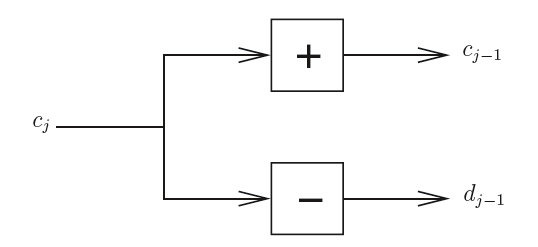
\includegraphics[width=7.47in]{images/multiscale_001} 

}

\caption{Generic step in multiscale transform.}\label{fig:unnamed-chunk-113}
\end{figure}

다중척도 변환은 다음과 같이 같은 차원의 새로운 벡터를 정의하는 과정으로
볼 수 있다. \[(1,1,7,9,2,8,8,6) \rightarrow (42,6,14,4,0,2,6,-2).\] 바뀐
벡터를 살펴보면, 42는 평균(global trend)에 해당되고, 6은 \(J=0\)일 때의
상세, \((14,4)\)는 \(J=1\)일 때의 상세, \((0,2,6,-2)\)는 \(J=2\)일 때의
상세이다. \(d_{j,k}\)는 \textbf{웨이블릿 계수(wavelet coefficient)}로,
\(c_{j,k}\)는 \textbf{압축 계수(scaling coefficient)} 또는
\textbf{부드러움 계수(smooth coefficient)}라 부른다. 여기서 \(j\)는
수준(level), 척도(scale), 또는 해상도(resolution)을 나타내며, \(k\)는
위치(location)를 나타낸다.

\section{역(inverse)}\label{inverse}

우리는 \(\{ d_{j,k} \}\)와 \(\{ c_{j,k} \}\)를 가지고 \(\mathbf{y}\)를
구할 수 있다. 이를 위해서는
\[c_{j-1,2k}=\frac{(c_{j-1,2k}+d_{j-2,k})}{2}, c_{j-1,2k-1}=\frac{(c_{j-1,2k}+-d_{j-2,k})}{2}\]
이 두 가지만 알고 있으면 된다.

\BeginKnitrBlock{example}[다중척도 역변환]
\protect\hypertarget{exm:unnamed-chunk-114}{}{\label{exm:unnamed-chunk-114}
\iffalse (다중척도 역변환) \fi{} }앞서 다룬 자료
\(\mathbf{y}=(1,1,7,9,2,8,8,6)\)를 생각해보자. 이것의 다중척도 변환
결과는
\((c_{01},d_{0,1},d_{11},d_{12},d_{21},d_{22},d_{23},d_{24})=(42,6,14,4,0,2,6,-2)\)였다.
이를 가지고 역변환을 해 보면,

\begin{eqnarray*}
c_{12}&=&\frac{(42+6)}{2}=24, c_{11}=\frac{(42-6)}{2}=18,\\
c_{24}&=&\frac{(24+4)}{2}=14, c_{23}=\frac{(24-4)}{2}=10, c_{22}=\frac{(18+14)}{2}=16, c_{21}=\frac{(18-14)}{2}=2,\\
c_{38}&=&\frac{(14-2)}{2}=6, c_{37}=\frac{(14+2)}{2}=8, c_{36}=\frac{(10+6)}{2}=8, c_{35}=\frac{(10-6)}{2}=2,\\
c_{34}&=&\frac{(16+2)}{2}=9, c_{33}=\frac{(16-2)}{2}=7, c_{32}=\frac{(2+0)}{2}=1, c_{31}=\frac{(2-0)}{2}=1.
\end{eqnarray*}

이다. 여기서 알 수 있는 사실 중 하나는 가장 섬세한 부드러움 계수는
데이터, 즉 자료라는 것이다.
\EndKnitrBlock{example}

그런데 데이터를 부드러움 계수로 다루는 것이 과역 적절한가? 라는 의문이
들 수 있다. 예를 들어, 자료에 잡음이 너무 많은 경우 부드러움 계수 또한
오류가 많이 생길 것이다. 통계학에서는 이를 보완하기 위해 \(\mathbf{y}\)
또는 \(d\)에 적절한 추정을 한 \(\hat{y}\) 또는 \(\hat{d}\) 등을
고려하기도 한다. (통계학자들은 데이터를 언제나 잡음이 끼어있는 신호라고
생각하고 있음을 명심해야 한다. 이 점이 통계학자와 다른 분야의 학자들이
자료를 보는 관점의 가장 큰 차이점 중 하나이다.)

\section{희소성(sparsity)}\label{sparsity}

\begin{figure}

{\centering 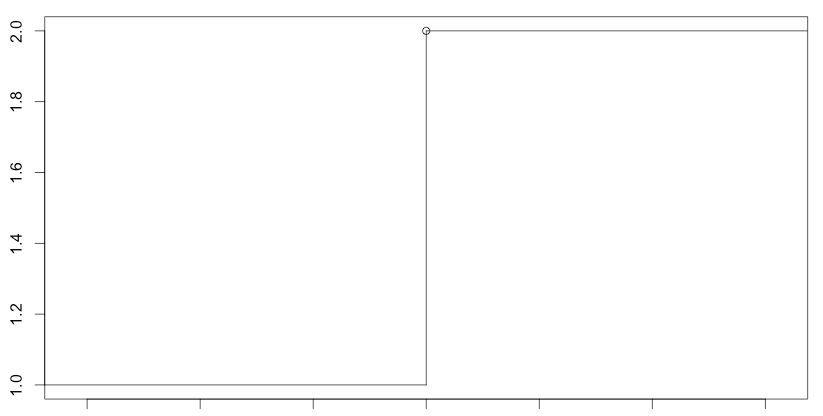
\includegraphics[width=11.43in]{images/multiscale_003} 

}

\caption{Example of sparse function.}\label{fig:unnamed-chunk-115}
\end{figure}

위 그림은 희소성을 갖는 함수의 전형적인 예 중 하나이다. 이 자료는 왼쪽은
항상 1, 오른쪽은 항상 2의 값을 갖고 있는 부드러운(smooth) 함수이며
변화가 없다. 그러나 가운데 지점에서는 함숫값이 1에서 2로 바뀌면서 급격한
점프가 일어난다. 이 지점은 다른 지역과는 달리 굉장히 다른 정보를 갖고
있는 것이다. 기존 회귀분석에서는 근본적인 함수(underlying function)들의
동질성(homogeneous) 가정을 바탕으로 분석한다. 이 말은 변동이 항상
일정하다는 뜻으로, 함수가 어떤 지역에서 두 번 미분 가능하면 다른
지역에서도 똑같이 두 번 미분 가능해야 한다는 것이다. 그러나 위 그림의
함수처럼 어떤 지역에서는 한 번만 미분 가능하거나 아예 미분 가능하지 않을
수도 있다. 이런 함수들을 다룰 때에는 다중척도 방법으로 접근하는 것이
필요하다.

\citep{Donoho1994}의 논문 이전까지 통계학자들의 관심사는 부드러운 함수의
평균 추정에 집중되어 있었다. Donoho는 논문에서 몇 가지 혁신적인 개념들을
제시했는데, 임계화(thresholding), \textbf{희소성(sparsity)} 등이
그것이다. 그의 아이디어는 당시에는 이해하기 힘든 것들이었다. 그러나 이
논문은 후대에 들에 고차원 자료 분석의 밑거름이 되게 해 주었고,
\textbf{least absolute sharinkage and selection operator (LASSO)}와 거의
같은 개념을 먼저 제시하였다. Donoho의 제자인 Fan은 후에 스승의
아이디어를 알기 쉽게 해석하여 \textbf{smoothly clipped absolute
deviation (SCAD)}라는 것을 제안하기도 하였다.

우리가 지금까지 일반적으로 배운 회귀분석 모형은 다음과 같이 나타낼 수
있다. \[y=f+\epsilon, \qquad{\epsilon \sim \mathcal{N}(0,\sigma^{2}).}\]
다시 말하면, 우리가 지금까지 다뤘던 모든 자료에는 오차(\(\epsilon\))와
\(f\)가 공존하는 형태의 모형이다. 이러한 모형에서는, 평균이 매우
중요하며 큰 의미를 갖게 된다. 그러나 성긴 모형에서는 상황이 조금
달라진다. 어떤 \(y\)는 \(f\)만 갖기도 하고, 또는 \(\epsilon\)만 갖기도
한다. \(\mathbf{y}=(y_{1},y_{2},y_{3},y_{4})\)라는 자료가 있을 때 이들
중 \(y_{3}\)만 \(f\)의 정보가 들어있는 진짜 신호이고 나머지
\(y_{1},y_{2},y_{4}\)는 잡음만 있을 수도 있는 것이다. 이런 자료에서 가장
좋은 추정량은 평균이 아니라 \(y_{3}\)이다.

\BeginKnitrBlock{theorem}[다중척도 변환의 희소성]
\protect\hypertarget{thm:unnamed-chunk-116}{}{\label{thm:unnamed-chunk-116}
\iffalse (다중척도 변환의 희소성) \fi{} } 다음과 같은 자료
\(\mathbf{y}=(1,1,1,1,2,2,2,2)\)를 생각해보자. 이 자료를 다중척도 변환해
보면 \[(1,1,1,1,2,2,2,2) \rightarrow (1,2,4,0,0,0,0,0)\] 과 같이 0이
많은 벡터로 변환될 것이다.
\EndKnitrBlock{theorem}

위 예제와 같이 0이 많이 있는 자료들을 \textbf{희소성(sparsity)}이 있는
자료라 하며, 다중척도 변환은 희소성이 있는 자료를 다룰 때 많은 도움이 될
수 있다.

\section{신호처리에서의 필터(filter in signal
processing)}\label{-filter-in-signal-processing}

이 절의 내용은 위키피디아의 것을 참조하였다. 신호처리에서
\textbf{필터(filter)}란 신호에서 원하지 않는 특징들을 제거해주는 장치다.
필터는

\begin{itemize}
\item
  linear or non-linear
\item
  time-invariant or time-variant
\item
  causal or not-causal: depending if present output depends or not on
  ``future'' input; of course, for time related signals processed in
  real-time all the filters are causal; it is not necessarily so for
  filters acting on space-related signals or for deferred-time
  processing of time-related signals.
\item
  analog or digital
\item
  discrete-time (sampled) or continuous-time
\item
  passive or active type of continuous-time filter
\item
  infinite impulse response (IIR) or finite impulse response (FIR) type
  of discrete-time or digital filter.
\end{itemize}

등으로 구분할 수 있다.

다음은 \textbf{선형 필터(linear filter)}에서 쓰이는 용어들이다. 여기서
원하지 않는 특징들은 주로 주파수를 의미하는 것이라 볼 수 있다.

\begin{figure}

{\centering 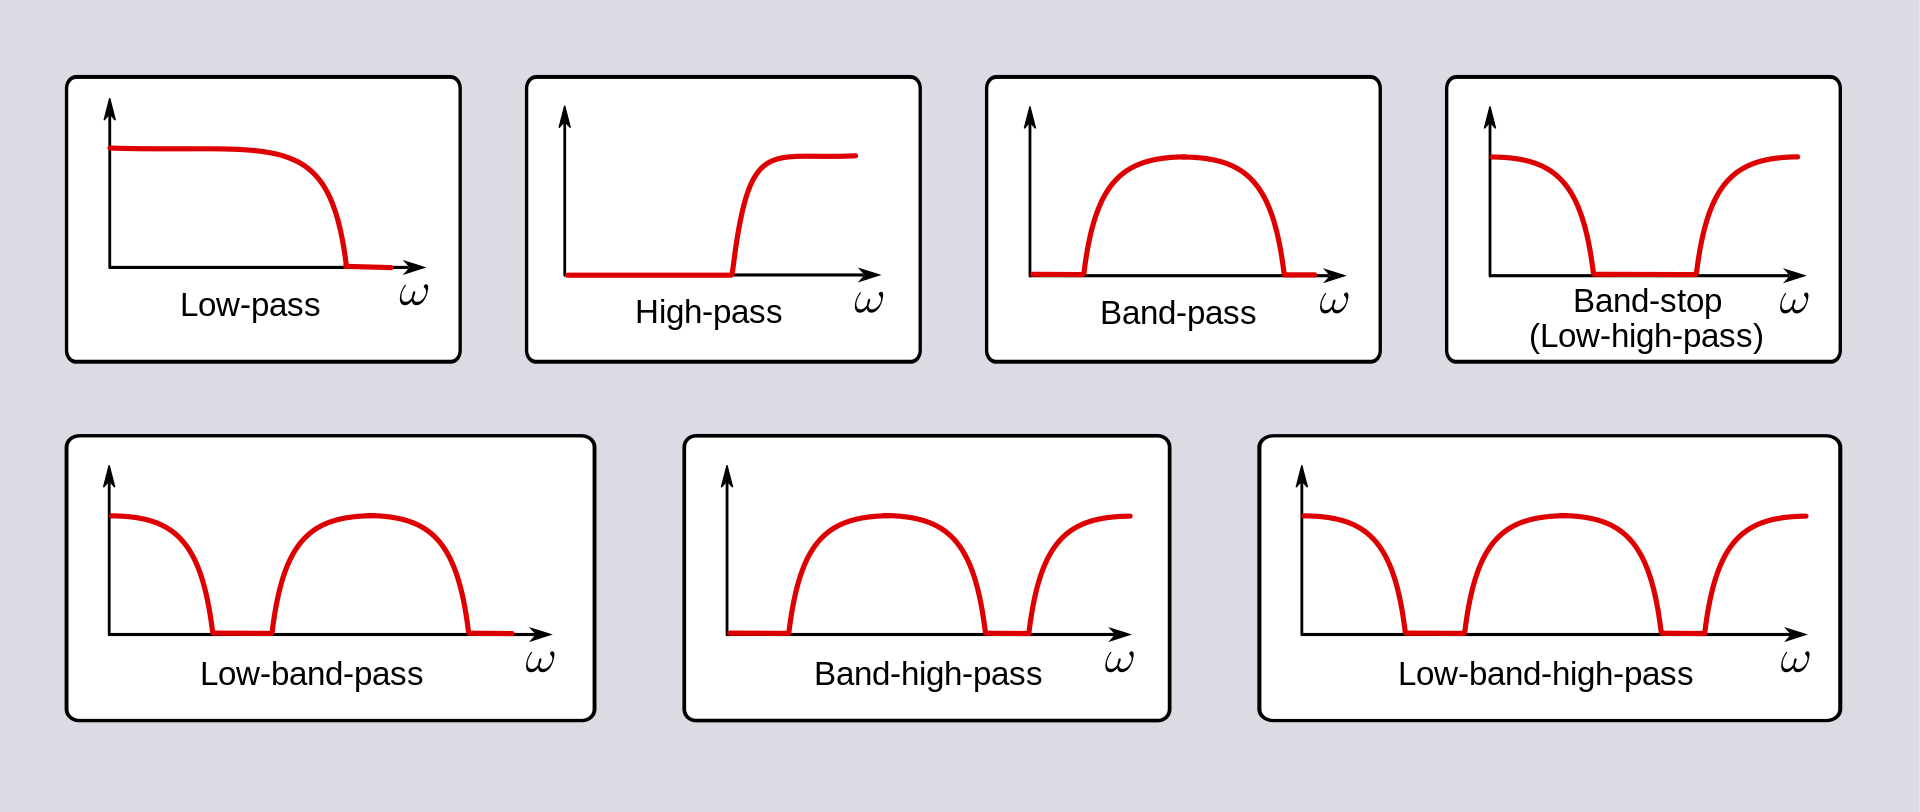
\includegraphics[width=26.67in]{images/multiscale_Bandform} 

}

\caption{Various forms of linear filters.}\label{fig:unnamed-chunk-117}
\end{figure}

\begin{itemize}
\item
  Low-pass filter -- 낮은 주파수는 통과시키고(low frequencies are
  passed), 높은 주파수는 감쇠, 즉 약하게 한다(high frequencies are
  attenuated).
\item
  High-pass filter -- 높은 주파수는 통과시키고(high frequencies are
  passed), 낮은 주파수는 감쇠하도록 한다(low frequencies are
  attenuated).
\item
  Band-pass filter -- only frequencies in a frequency band are passed.
\item
  Band-stop filter or band-reject filter -- only frequencies in a
  frequency band are attenuated.
\item
  Notch filter -- rejects just one specific frequency - an extreme
  band-stop filter.
\item
  Comb filter -- has multiple regularly spaced narrow passbands giving
  the bandform the appearance of a comb.
\item
  All-pass filter -- all frequencies are passed, but the phase of the
  output is modified.
\item
  Cutoff frequency is the frequency beyond which the filter will not
  pass signals. It is usually measured at a specific attenuation such as
  3 dB.
\item
  Roll-off is the rate at which attenuation increases beyond the cut-off
  frequency.
\item
  Transition band, the (usually narrow) band of frequencies between a
  passband and stopband.
\item
  Ripple is the variation of the filter's insertion loss in the
  passband.
\end{itemize}

\section{선형 필터(linear filter)}\label{-linear-filter}

이 절의 내용은 \citep{Shumway2010}를 참고하였다. 여기서는 선형 필터가
시계열로부터 신호를 어떻게 뽑아내는지에 대해 설명한다. 선형 필터는
시계열 자료의 스펙트럼 특성을 변형시켜 예측 가능하게끔 한다고 한다.

선형필터는 특정화한 계수들 \(a_{j}, j=0,\pm 1, \pm 2, \ldots\)를
사용한다. 이것은 투입된 시계열 \(x_{t}\)를 다음 관계를 통해
\[y_{t}=\sum_{j=-\infty}^{\infty}a_{j}x_{t-j}, \sum_{j=-\infty}^{\infty}|a_{j}| <\infty\]
\(y_{t}\)라는 시계열로 변화시킨다. 통계 용어로 이 식은 convolution에
해당한다. 이 계수들은 특별히 \textbf{임펄스 응답 함수(impulse response
function)}이라고 부른다.

\section{R 예제(R-multiscale)}\label{r-r-multiscale}

웨이블릿과 관련된 R 예제를 담고 있는 책은 \citep{Nason2010}이 있다. 이
책의 저자는 \texttt{wavethresh}란 R 패키지를 만들기도 했다. 또 다른 R
패키지로 \texttt{waveslim}이라는 것도 있다. 여기서는 \citep{Nason2010}의
예제를 일부 다뤄보기로 한다.

\texttt{wavethresh} 라이브러리를 실행시킨 상황에서, 다음 벡터의 웨이블릿
변환을 실행해본다. \texttt{wd}라는 함수가 이를 가능케 해 준다.
\texttt{wr}이라는 함수는 reconstruction을 시킨다.

\begin{Shaded}
\begin{Highlighting}[]
\NormalTok{y <-}\StringTok{ }\KeywordTok{c}\NormalTok{(}\DecValTok{1}\NormalTok{,}\DecValTok{1}\NormalTok{,}\DecValTok{7}\NormalTok{,}\DecValTok{9}\NormalTok{,}\DecValTok{2}\NormalTok{,}\DecValTok{8}\NormalTok{,}\DecValTok{8}\NormalTok{,}\DecValTok{6}\NormalTok{)}
\NormalTok{## wd: wavelet transform}
\NormalTok{ywd <-}\StringTok{ }\KeywordTok{wd}\NormalTok{(y, }\DataTypeTok{filter.number=}\DecValTok{1}\NormalTok{, }\DataTypeTok{family=}\StringTok{"DaubExPhase"}\NormalTok{)}
\KeywordTok{names}\NormalTok{(ywd)}
\end{Highlighting}
\end{Shaded}

\begin{verbatim}
> [1] "C"        "D"        "nlevels"  "fl.dbase" "filter"   "type"    
> [7] "bc"       "date"
\end{verbatim}

\begin{Shaded}
\begin{Highlighting}[]
\NormalTok{## what filter produced a particular wavelet decomposition object}
\NormalTok{ywd$filter}
\end{Highlighting}
\end{Shaded}

\begin{verbatim}
> $H
> [1] 0.7071068 0.7071068
> 
> $G
> NULL
> 
> $name
> [1] "Haar wavelet"
> 
> $family
> [1] "DaubExPhase"
> 
> $filter.number
> [1] 1
\end{verbatim}

\begin{Shaded}
\begin{Highlighting}[]
\NormalTok{## level 2 detail coefficients}
\KeywordTok{accessD}\NormalTok{(ywd, }\DataTypeTok{level=}\DecValTok{2}\NormalTok{)}
\end{Highlighting}
\end{Shaded}

\begin{verbatim}
> [1]  0.000000 -1.414214 -4.242641  1.414214
\end{verbatim}

\begin{Shaded}
\begin{Highlighting}[]
\NormalTok{## plot wavelet decomposition coefficients}
\KeywordTok{plot}\NormalTok{(ywd)}
\end{Highlighting}
\end{Shaded}

\begin{figure}

{\centering 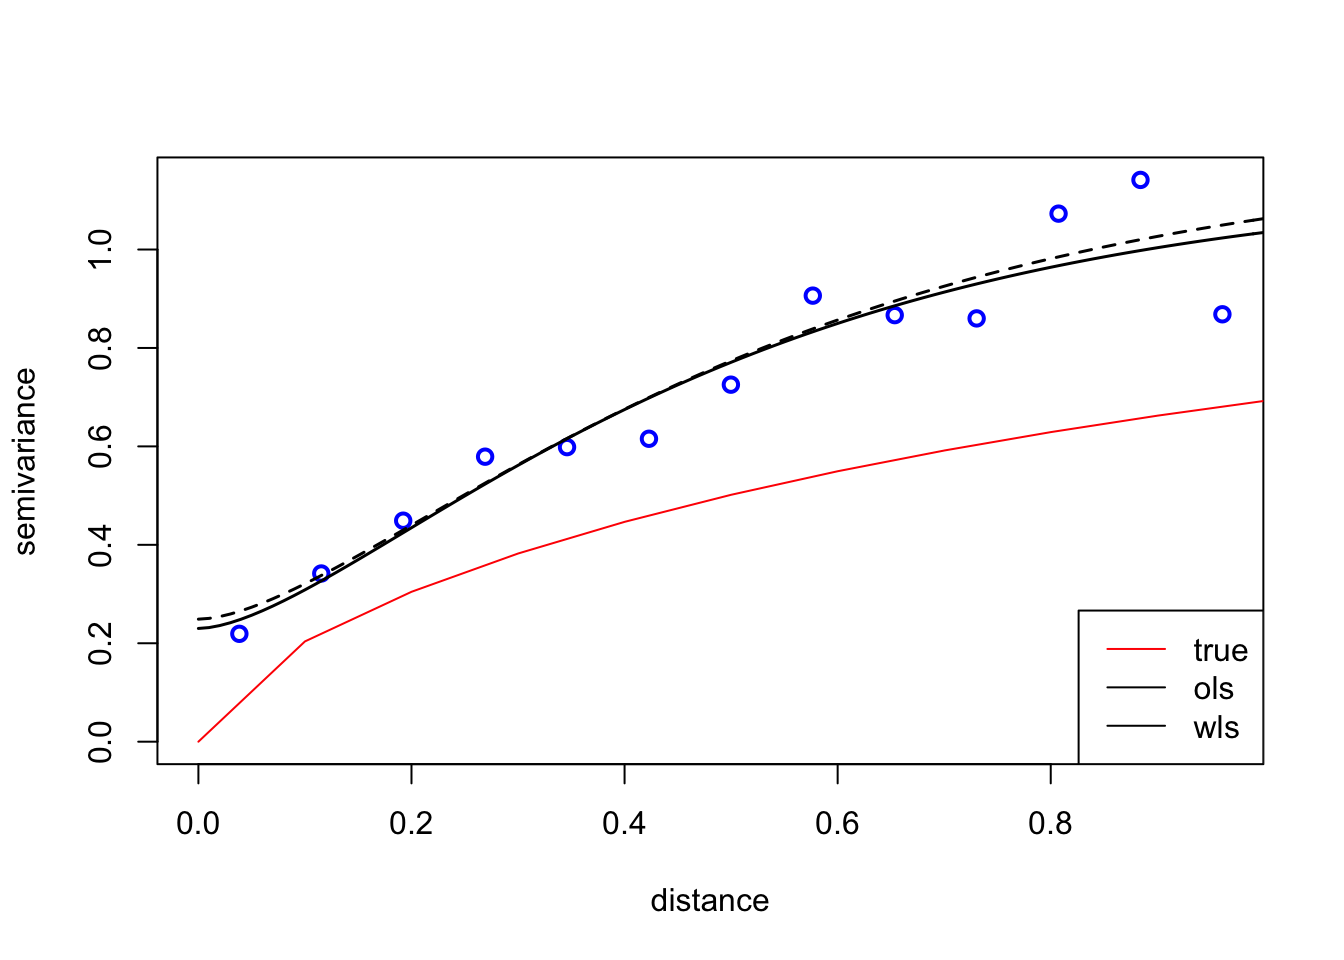
\includegraphics{book_files/figure-latex/unnamed-chunk-119-1} 

}

\caption{Wavelet decomposition coefficients.}\label{fig:unnamed-chunk-119}
\end{figure}

\begin{verbatim}
> [1] 7 7 7
\end{verbatim}

\begin{Shaded}
\begin{Highlighting}[]
\NormalTok{## wr: wavelet reconstruction}
\KeywordTok{wr}\NormalTok{(ywd)}
\end{Highlighting}
\end{Shaded}

\begin{verbatim}
> [1] 1 1 7 9 2 8 8 6
\end{verbatim}

\chapter{웨이블릿 변환}\label{wavelettransform}

웨이블릿은 'Wave'와 프랑스어 'let'의 합성어로, 'let'은 'small'이라는
뜻을 가지고 있다. 즉 웨이블릿은 'small wave'라는 뜻으로, \textbf{컴팩트
받침(compactly supported)}인 함수들을 일컷는 말이다. 사인(Sine),
코사인(cosine) 기저(basis)는 \((-\infty, \infty)\)에서 정의되는 매우 큰
파동이므로 웨이블릿에 해당하지 않는다.

\textbf{웨이블릿 변환(wavelet transform)}이란 웨이블릿 기저함수를 이용해
데이터를 변환하는 것을 말한다. 여기서 웨이블릿 기저함수라는 건 적분하면
0이 되고, 진동하면서 진폭이 0으로 수렴하는 함수를 말한다.

\section{이산 Haar 웨이블릿 변환(discrete Haar wavelet
transform)}\label{-haar--discrete-haar-wavelet-transform}

가장 단순한 웨이블릿 변환으로 \textbf{Haar 웨이블릿 변환(Haar wavelet
transform)}이 있다.

앞서 상세와 성김은 다음과 같이 구할 수 있었음을 상기하자.
\[d_{k}=y_{2k}-y_{2k-1}, c_{k}=y_{2k}+y_{2k-1}.\] 에너지를 보존하기 위해
다음과 같이 \(\alpha\)라는 상수를 고려하자.
\[d_{k}=\alpha(y_{2k}-y_{2k-1}), c_{k}=\alpha(y_{2k}+y_{2k-1}).\] 그러면

\begin{eqnarray*}
d_{k}^{2}+c_{k}^{2}&=&\alpha^{2}(y_{2k}^{2}-2y_{2k}y_{2k-1}+y_{2k-1}^{2}+\alpha^{2}(y_{2k}^{2}+2y_{2k}y_{2k-1}+y_{2k-1}^{2})\\
&=&2\alpha^{2}(y_{2k}^{2}+y_{2k-1}^{2})
\end{eqnarray*}

즉 \(2\alpha^{2}=1 \Rightarrow \alpha=\frac{1}{\sqrt{2}}\)이면 \(y\)와
\(d\)의 에너지가 보존(conserved)된다. 이렇게
\[d_{k}=\frac{1}{\sqrt{2}}(y_{2k}-y_{2k-1}), c_{k}=\frac{1}{\sqrt{2}}(y_{2k}+y_{2k-1}).\]
하는 것을 \textbf{표준화(normalization)}라고 말하기도 한다. 정리하면
\textbf{Haar 웨이블릿 변환(Haar wavelet transform)}의 \textbf{이산
웨이블릿 계수(discrete wavelet coefficient)} \(d_{k}\)는
\[d_{k}=g_{0}y_{2k}+g_{1}y_{2k-1}=\sum_{l=-\infty}^{\infty}g_{l}y_{2k-l}\]
이며 여기서 \[
g_{l} = 
\begin{cases}
\frac{1}{\sqrt{2}} & \text{if $l=0$} \\
-\frac{1}{\sqrt{2}} & \text{if $l=1$}\\
0 & \text{o.w.}\\
\end{cases}
\]

여기서 \(g_{l}\)을 \textbf{고역 필터(high-pass filter)}라고 부른다.
마찬가지로 성김에 대해서도 \[
c_{k}=
\sum_{l=-\infty}^{\infty}h_{l}y_{2k-l},
h_{l} = 
\begin{cases}
\frac{1}{\sqrt{2}} & \text{if $l=0$}\\
\frac{1}{\sqrt{2}} & \text{if $l=1$}\\
0 & \text{o.w.}
\end{cases}
\] 로 나타낼 수 있고 \(h_{l}\)을 \textbf{저역 필터(low-pass filter)}라
부른다.

세부와 성김은 앞서 언급한 피라미드 알고리즘으로 구할 수도 있지만
여기서는 \(\mathbf{d}=\mathbf{Wy}\)처럼 통계학자들에게 익숙한 행렬 꼴로
바꾸어 표현한다.

\BeginKnitrBlock{example}[행렬을 이용한 웨이블릿 계수의 계산]
\protect\hypertarget{exm:unnamed-chunk-120}{}{\label{exm:unnamed-chunk-120}
\iffalse (행렬을 이용한 웨이블릿 계수의 계산) \fi{} }행렬을 이용해
웨이블릿 계수를 계산해보자. 다음과 같은 자료
\(\mathbf{y}=(1,1,7,9,2,8,8,6)\)에 행렬 \(W\)을 다음과 같이 정의하면

\[
W =
\begin{bmatrix}
\frac{\sqrt{2}}{4} & \frac{\sqrt{2}}{4} & \frac{\sqrt{2}}{4} & \frac{\sqrt{2}}{4} & \frac{\sqrt{2}}{4} & \frac{\sqrt{2}}{4} & \frac{\sqrt{2}}{4} & \frac{\sqrt{2}}{4}\\
\frac{1}{\sqrt{2}} & -\frac{1}{\sqrt{2}} & 0 & 0 & 0 & 0 & 0 & 0\\
 0 & 0 & \frac{1}{\sqrt{2}} & -\frac{1}{\sqrt{2}} & 0 & 0 & 0 & 0\\
 0 & 0 & 0 & 0 &  \frac{1}{\sqrt{2}} & -\frac{1}{\sqrt{2}} & 0 & 0\\
 0 & 0 & 0 & 0 & 0 & 0 &  \frac{1}{\sqrt{2}} & -\frac{1}{\sqrt{2}}\\
 \frac{1}{2} & \frac{1}{2} & -\frac{1}{2} & -\frac{1}{2} & 0 & 0 & 0 & 0 \\
 0 & 0 & 0 & 0 &  \frac{1}{2} & \frac{1}{2} & -\frac{1}{2} & -\frac{1}{2}\\
 \frac{\sqrt{2}}{4} & \frac{\sqrt{2}}{4} & \frac{\sqrt{2}}{4} & \frac{\sqrt{2}}{4} & -\frac{\sqrt{2}}{4} & -\frac{\sqrt{2}}{4} & -\frac{\sqrt{2}}{4} & -\frac{\sqrt{2}}{4}\\
\end{bmatrix}
\]

\(\mathbf{d}=(\frac{21\sqrt{2}}{2},0,-\sqrt{2},-3\sqrt{2},\sqrt{2},-7,-2,\frac{3\sqrt{2}}{2})\)를
얻을 수 있다. (이 예제에서는 \citep{Nason2010}의 정의를 따라갔다.)
\EndKnitrBlock{example}

위 예제의 \(W\)처럼 Haar 웨이블릿의 \(W\)는
\textbf{정규직교(orthonormal)}라는 성질을 갖는데, 정규직교의 의미는
\(W^{T}W=I\)이다. 그러나 모든 웨이블릿의 \(W\)가 정규직교인 것은 아니다.
그리고
\[\| \mathbf{d} \|^{2}=\mathbf{d}^{T}\mathbf{d}=(W\mathbf{y})^{T}(W\mathbf{y})=\mathbf{y}^{T}W^{T}W\mathbf{y}=\| \mathbf{y} \|^{2}.\]
이 식은 \textbf{Parseval 등식(Parseval's identity)}에 대응된다.

정규직교인 웨이블릿의 \(W\)은 다음과 같은 장점을 갖는다. 다음과 같이
원래 자료와 추정량에 대한 공식이 다음과 같이 주어졌을 때,
\[y=f+\epsilon, \epsilon \sim (\cdot, \sigma^{2}I) \rightarrow d=\theta +e, Wy=d, Wf=\theta, W\epsilon=e\]
정규직교인 \(W\)이면
\[Var(W\epsilon)=WVar(\epsilon)W^{T}=\sigma^{2}I=Var(\epsilon)\] 이다.
즉 원래 자료와 추정량의 분산 구조가 같다.

\section{압축계수(scaling coefficient)와 전이계수(translation
coefficient) 개념}\label{scaling-coefficient-translation-coefficient-}

\(p(x)\)라는 함수가 주어졌을 때, 이것의 \textbf{압축 및 전이된
버전(scaled and translated version)}은 다음과 같이 정의된다.

\[p_{j,k}(x)=2^{\frac{j}{2}}p(2^{j}x-k)\]

\[
\| p_{j,k}(x) \|^{2}=\int_{\infty}^{\infty}p_{j,k}^{2}(x)dx=\int_{\infty}^{\infty}2^{j}p^{2}(2^{j}x-k)dx=\int_{\infty}^{\infty}p^{2}(y)dy=\| p(y) \|^{2}
\]

\section{섬세한 척도 근사(fine-scale
approximation)}\label{--fine-scale-approximation}

다음과 같이 \textbf{Haar 함수(Haar function)}를 정의한다.

\[
\phi(x) = 
\begin{cases}
1 & \text{if $x \in [0,1]$}\\
0 & \text{o.w.}
\end{cases}
\]

\begin{figure}

{\centering 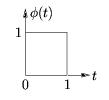
\includegraphics[width=1.51in]{images/multiscale_004} 

}

\caption{Plot of Haar function.}\label{fig:unnamed-chunk-121}
\end{figure}

이 때 \(\phi(x)=\phi_{0,0}(x)\)이다. 즉 척도도 바꾸지 않고 어떤
전이(translation)도 없을 때의 \(\phi\)인 것이다.

\begin{figure}

{\centering 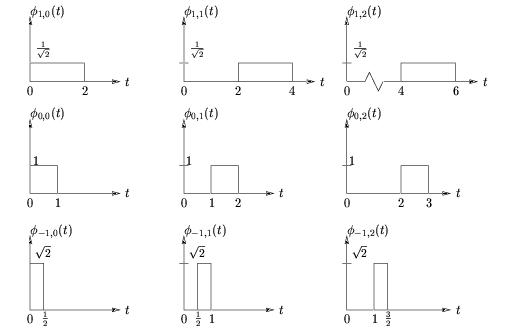
\includegraphics[width=7.1in]{images/multiscale_005} 

}

\caption{Scaling and translation version of Haar function.}\label{fig:unnamed-chunk-122}
\end{figure}

가장 섬세한 레벨의 (Haar) \textbf{척도 웨이블릿(scaling wavelet, father
wavelet)}은
\[c_{J,k}=\int f(x) \phi_{J,k}(x)dx=\int f(x) 2^{\frac{J}{2}}\phi(2^{J}x-k)dx\]
이다. 이것은 앞서 말한 \(p\)를 \(\phi\)로 바꾸면 되며 또한 데이터와
같음을 알고 있다. 그리고 앞의 정의들을 이용하면

\[
\phi_{J,k} =
\begin{cases}
2^{\frac{J}{2}} & \text{if $x \in [2^{-J}k,2^{-J}(k+1)]$}\\
0 & \text{o.w.}
\end{cases}
\]

이다. 여기서 정의하는 간격을 \(I_{J,k}\)라 한다. 우리는 다양한 척도에서
\(f\)를 근사할 수 있다. 가장 섬세한 척도로는
\[f_{J}=\sum_{k=0}^{2^{J}-1}c_{J,k}\phi_{J,k}(x)\] 가 있으며, 가장 성긴
척도로 근사하고 싶으면
\[f_{0}=\sum_{k=0}^{2^{0}-1}c_{0,k}\phi_{J,k}(x)\] 로 \(f\)를 근사한다.

\section{섬세한 척도로부터 성긴 척도 계수의 계산(computing coarser scale
coefficients from fine
scale)}\label{-----computing-coarser-scale-coefficients-from-fine-scale}

앞에서 말한대로, 우리는 섬세한 척도의 계수들로부터 좀 더 성긴 척도의
계수들을 구할 수 있다.

\begin{eqnarray*}
c_{J-1,k}&=&\int_{2^{-(J-1)}k}^{2^{-(J-1)}(k+1)}f(x)\phi_{J-1,k}(x)dx\\
&=&\int_{2^{-J}(2k)}^{2^{-J}(2k+2)}f(x)2^{(\frac{J-1}{2})}\phi(2^{J-1}x-k)dx\\
&=&2^{-\frac{1}{2}}\int_{2^{-J}(2k)}^{2^{-J}(2k+2)}f(x)2^{\frac{J}{2}}\phi(2^{J-1}x-k)dx\\
&=&2^{-\frac{1}{2}}[\int_{2^{-J}(2k)}^{2^{-J}(2k+2)}f(x)2^{\frac{J}{2}}\phi(2^{J}x-2k)dx + \int_{2^{-J}(2k)}^{2^{-J}(2k+2)}f(x)2^{\frac{J}{2}}\phi(2^{J}x-2k-1)dx]\\
&=&2^{-\frac{1}{2}}(c_{J,2k}+c_{J,2k+1}).\\
\end{eqnarray*}

즉 \({J-1}\)척도 계수는 \(J\)척도 계수로부터 구할 수 있다. 여기서 중간에
\[\phi(x)=\phi(2x)+\phi(2x-1)\] 이라는 사실을 이용하였는데, 이것은 매우
중요하다. 이것을 \textbf{척도방정식(two-scale relationship)} 또는
\textbf{팽창방정식(dilation relationship)}이라고 한다.

\begin{figure}

{\centering 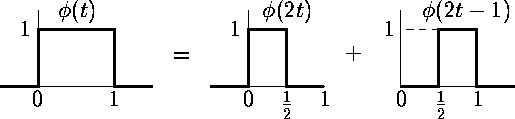
\includegraphics[width=7.15in]{images/multiscale_006} 

}

\caption{Relationship between Haar scale function.}\label{fig:unnamed-chunk-123}
\end{figure}

\section{척도 근사들 사이의 차이(defference between scale
approximations)(이를 웨이블릿이라
부름)}\label{---defference-between-scale-approximations--}

척도 근사들의 차이에서 도출된 함수들이 작은 파도(small wave) 형태를
띄므로 이것을 웨이블릿이라 부른다. 앞서 근사식
\(f_{J}=\sum_{k=0}^{2^{J}-1}c_{J,k}\phi_{J,k}(x)\)과
\(p_{j,k}(x)=2^{\frac{j}{2}}p(2^{j}x-k)\)으로부터 \(J=1\)일 때에는 \[
f_{1}(x)=c_{10}\phi_{10}(x)+c_{11}\phi_{11}(x)=c_{10}2^{\frac{1}{2}}\phi(2x)+c_{11}2^{\frac{1}{2}}\phi(2x-1)
\] 이다. 여기서 \(f_{0}(x)=c_{00}\phi_{00}(x)\)라 하고
\(c_{J-1,k}=\frac{c_{J,2k}+c_{J,2k-1}}{\sqrt{2}}\)를 이용하면

\begin{eqnarray*}
f_{1}(x)-f_{0}(x)&=&c_{10}\phi_{10}(x)+c_{11}\phi_{11}(x)-c_{00}\phi_{00}(x)\\
&=&c_{10}2^{\frac{1}{2}}\phi(2x)+c_{11}2^{\frac{1}{2}}\phi(2x-1)-c_{00}(\phi(2x)+\phi(2x-1))\\
&=&(c_{10}2^{\frac{1}{2}}-c_{00})\phi(2x)+(c_{11}2^{\frac{1}{2}}-c_{00})\phi(2x-1)\\
&=&(\frac{c_{10}-c_{11}}{\sqrt{2}})\phi(2x)-(\frac{c_{10}-c_{11}}{\sqrt{2}})\phi(2x-1)\\
&=&(\frac{c_{10}-c_{11}}{\sqrt{2}})(\phi(2x)-\phi(2x-1))\\
&=&d_{00}\psi(x).\\
\end{eqnarray*}

여기서 \((\frac{c_{10}-c_{11}}{\sqrt{2}})\)은 웨이블릿 상수에 해당하고,
\(\psi(x)=\phi(2x)-\phi(2x-1)\)은 \textbf{Haar 모웨이블릿(Haar mother
wavelet)}이라고 한다.

\[
\psi(x) = 
\begin{cases}
1 & \text{if $x \in [0,\frac{1}{2})$}\\
-1 & \text{if $x \in [\frac{1}{2},1)$}\\
0 & \textrm{o.w.}
\end{cases}
\]

\begin{figure}

{\centering 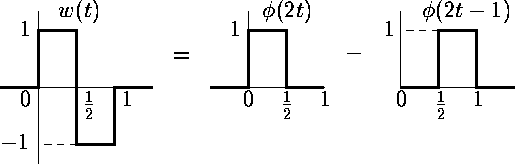
\includegraphics[width=7.15in]{images/multiscale_007} 

}

\caption{Haar mother wavelet function.}\label{fig:unnamed-chunk-124}
\end{figure}

우리는 웨이블릿을 가지고 어떤 함수를 분해(decompose)할 수 있다. 앞의
결과는 \[
f_{1}(x)=f_{0}(x)+d_{00}\psi(x)=c_{00}\phi(x)+d_{00}\psi(x)
\]

로 쓸 수 있으며 \(f_{1}\)을 좀 더 성긴 척도함수인 \(f_{0}\)과
차이(difference)에 해당하는 \(\psi(x)\)로 분해할 수 있음을 보여준다.
일반적으로 \(f_{j+1}(x)\)는 다음과 같이 쓸 수 있다.

\begin{eqnarray*}
f_{j+1}(x)&=&\sum_{k=0}^{2^{j}-1}c_{jk}\phi_{jk}(x)+\sum_{k=0}^{2^{j}-1}d_{jk}\psi_{jk}(x)\\
&=&f_{j}(x)+g_{j}(x)\\
&=&f_{j-1}(x)+g_{j-1}(x)+g_{j}(x)\\
&=& \vdots \\
&=&f_{0}(x)+\sum_{l=0}^{j}g_{l}(x).\\
\end{eqnarray*}

즉 \(f_{j+1}(x)\)은 가장 성긴 근사함수인 \(f_{0}\)와 각 수준에서의
차이인 \(g_{l}\)들의 합으로 표현할 수 있다.

\section{웨이블릿의 종류들(types of wavelets)}\label{-types-of-wavelets}

\subsection{Haar 웨이블릿(Haar wavelet)}\label{haar-haar-wavelet}

다음과 같이 \textbf{Haar 함수(Haar function)}의 정의를 다시 상기하자. \[
\phi(x) =
\begin{cases}
1 & \text{if $x \in [0,1]$}\\
0 & \text{o.w.}
\end{cases}
\]

\(x\)를 \textbf{물리적 영역(physical domain)} 또는 \textbf{시간
영역(time domain, t)}이라 생각하면, 시간에 대해 컴팩트 받침(compactly
supported)인 함수이다. 우리의 궁금점은 이 함수과 과연 \textbf{주파수
영역(frequency domain)}에서도 컴팩트 받침인가이다.

\BeginKnitrBlock{definition}[유니터리 푸리에 변환]
\protect\hypertarget{def:unnamed-chunk-125}{}{\label{def:unnamed-chunk-125}
\iffalse (유니터리 푸리에 변환) \fi{} } 주어진 함수의
\textbf{각진동수(angular frequency)를 이용한 유니터리 푸리에
변환(Fourier transform with unitary and angular frequency)}은 다음과
같다.
\[\hat{f}(\omega)=\frac{1}{\sqrt{2\pi}}\int_{-\infty}^{\infty}f(x)e^{-i\omega x}dx\]

여기서 \(\frac{1}{\sqrt{2\pi}}\)는 이 변환을 유니터리 푸리에 변환으로
만들기 위해 곱해지는 상수이다. 유니터리 변환과 푸리에 변환에 대한 보다
자세한 나용은 인터넷을 참조하기 바란다.
\EndKnitrBlock{definition}

앞서 나온 푸리에 변환을 이용해 Haar 함수를 푸리에 변환한 결과는 다음과
같다.
\[\hat{\phi}(\omega)=\frac{1}{\sqrt{2\pi}}e^{-\frac{i\omega}{2}}\text{sinc}(\frac{\omega}{2}).\]
여기서 \[
\text{sinc}(\omega)=
\begin{cases}
\frac{\sin (\omega)}{\omega} & \text{if $\omega \neq 0$}\\
1 &\text{if $\omega = 0$}
\end{cases}
\]

이다. \(\hat{\phi}(\omega)\)는 \(| \omega |^{-1}\)만큼의 감쇠(decay)를
가지며 꼬리가 굉장히 긴 함수이다. 즉 주파수 영역에서 이 함수는 컴팩트
받침과 거리가 먼 함수가 된다. 시간 영역과 주파수 영역 사이에 불확정성
원리(uncertainty principle)이 있다는 것은 알려진 사실이다.

\begin{figure}

{\centering 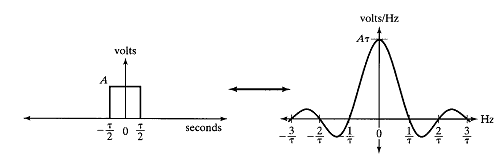
\includegraphics[width=6.96in]{images/multiscale_008} 

}

\caption{Haar function (left) and Haar function in frequency domain after Fourier transform (right).}\label{fig:unnamed-chunk-126}
\end{figure}

\section{데시메이티드되지 않은 웨이블릿(non-decimated
wavelets)}\label{--non-decimated-wavelets}

\chapter{일반적인 웨이블릿 변환}\label{generalDWT}

\section{일반적인 이산 웨이블릿 변환(the general fast
DWT)}\label{---the-general-fast-dwt}

앞선 내용들에서는 어떻게 성긴 스케일의 Haar 웨이블릿 계수들을 구하는지에
대해 설명했다. 여기서는 좀 더 일반적인 경우에 대해 설명한다.

\subsection{이산웨이블릿 변환에서의 전방변환(the forward transform in
DWT)}\label{--the-forward-transform-in-dwt}

다음과 같은 함수 \(f(x)\in L^{2}(\mathbb{R})\)이 있다고 하자. 그러면
레벨 \(J\)의 웨이블릿 계수로부터 레벨 \(J-1\)의 웨이블릿 계수를 어떻게
구할 수 있을까? 일단 다시한 번 \(J-1\) 레벨의 척도웨이블릿 (또는
부웨이블릿) \(c\)를 구하는 방법에 대해 생각해보자.

\begin{equation}\label{eq:fatherj1}
c_{J-1,k}=\int_{\mathbb{R}}f(x)\phi_{J-1,k}(x)dx
\end{equation}

왜냐하면 \(\{ \phi_{J-1,k(x)}\}_{k}\)가 \(V_{j-1}\)의 직교정규기저이기
때문이다. (?) (\(\phi\): 척도함수 또는 부웨이블릿) 이제 \(J-1\) 레벨의
\(\phi_{J-1,k}(x)\)를 \(\phi_{J,l}(x)\)와 dilation eqn
\(\phi(x)=\sum_{n\in\mathbb{Z}}h_{n}\phi_{1n}(x)\)를 이용해 나타내보자.

\begin{eqnarray}\label{eq:fatherj2}
\phi_{J-1,k}(x)&=&s^{(J-1)/2}\phi(2^{J-1}x-k)\nonumber\\
&=&2^{(J-1)/2}\sum_{n}h_{n}\phi_{1,n}(2^{J-1}x-k)\nonumber\\
&=&2^{(J-1)/2}\sum_{n}h_{n}2^{1/2}\phi\{2(2^{J-1}x-k)-n\}\nonumber\\
&=&2^{J/2}\sum_{n}h_{n}\phi(2^{J}x-2k-n)\nonumber\\ 
&=&\sum_{n}h_{n}\phi_{J,n+2k}(x).
\end{eqnarray}

이 때 위 식에 (\eqref{eq:fatherj1})을 넣으면

\begin{eqnarray}\label{eq:fatherj3}
c_{J-1,k}&=&\int_{\mathbb{R}}f(x)\sum_{n}h_{n}\phi_{J,n+2k}(x)dx\nonumber\\
&=&\sum_{n}h_{n}\int_{\mathbb{R}}f(x)\phi_{J,n+2k}(x)dx\nonumber\\
&+&\sum_{n}h_{n}c_{J,n+2k}
\end{eqnarray}

이며, 약간 re-arrange하면

\begin{equation}\label{eq:fatherj4}
c_{J-1,k}=\sum_{n}h_{n-2k}c_{J,n}
\end{equation}

으로 쓸 수 있다. 같은원리로

\begin{equation}\label{eq:motherj1}
d_{J-1,k}=\sum_{n}g_{n-2k}c_{J,n}
\end{equation}

을 얻을 수 있다고 한다.

\subsection{Filtering, dyadic decimation,
downscaling}\label{filtering-dyadic-decimation-downscaling}

앞서 언급한 (\eqref{eq:fatherj4}), (\eqref{eq:motherj1})을 다른 방법으로
생각해 볼 수도 있다. 예를 들면, 우리는 (\eqref{eq:fatherj4})와 같은 결과를
처음에 수열 \(\{c_{J,n}\}\)에 대해 \(\{h_{n}\}\)이라는 필터를
적용함으로써 \[c_{J-1,k}^{*}=\sum_{n}h_{n-k}c_{J,n}\] 이라는 결과를 얻을
수 있다는 것이다. 이는 일반적인 convolution 식이다. 여기서 'every other
one'을 pick해 \(c_{J-1,k}=c_{J-1,2k}^{*}\)을 만드는 것이다. 이 연산을
\textbf{이진 데시메이션(dyadic decimation)}이라고 한다(by an integer
factor of 2).

\BeginKnitrBlock{definition}[이진 데시메이션]
\protect\hypertarget{def:unnamed-chunk-127}{}{\label{def:unnamed-chunk-127}
\iffalse (이진 데시메이션) \fi{} }\textbf{(even dyddic decimation
operator)} 어떤 수열 \(x_{i}\)에 대한 \textbf{(even) dyadic decimation
operator} \(\mathcal{D}_{0}\)는 \[(\mathcal{D}_{0}x)_{l}=x_{2l}\] 로
정의한다.
\EndKnitrBlock{definition}

그러면 식 (\eqref{eq:fatherj4})와 (\eqref{eq:motherj1})는 (even) dyadic
decimation operator를 활용해
\[c_{J-1}=\mathcal{D}_{0}\mathcal{H}c_{J} \text{ and } d_{J-1}=\mathcal{D}_{0}\mathcal{G}c_{J}\]
로 나타낼 수 있다. 이 때 \(\mathcal{H}\)와 \(\mathcal{G}\)는
\textbf{regular filtering operation}을 나타낸다. 이러한 연산자의 사용은
식의 표현을 좀 더 효율적으로 만든다.

이를 응용해, DWT 계수들의 whole set은
\[d_{j}=\mathcal{D}_{0}\mathcal{G}(\mathcal{D}_{0}\mathcal{H})^{J-j-1}c_{J},\]
\[c_{j}=(\mathcal{D}_{0}\mathcal{H})^{J-j}c_{J}\] 로 표현할 수 있다.
(\(j=0,\ldots , J-1\)) 이 때 \(d_{j}\), \(c_{j}\)는 길이 \(2^{j}\)인
벡터임을 상기하자.

\subsection{최초의 부웨이블릿 계수 얻어내기(obtaining the initial
fine-scale father
coefficients)}\label{---obtaining-the-initial-fine-scale-father-coefficients}

\begin{enumerate}
\def\labelenumi{\arabic{enumi}.}
\item
  deterministic approach (특별하지 않으면 이것을 사용)
\item
  stochastic approach
\end{enumerate}

\subsection{역 이산 웨이블릿 변환(inverse discrete wavelet
transform)}\label{---inverse-discrete-wavelet-transform}

\section{엡실론-데시메이티드 웨이블릿 변환(the epsilon-decimated wavelet
transform)}\label{---the-epsilon-decimated-wavelet-transform}

(Wavelet methods in statistics with R 57쪽)

Dyadic decimation \(\mathcal{D}_{0}\)는 벡터의 even element들만을
pick하게 된다. 그런데 반대로 벡터의 모든 odd element들만 이용해서
연산자를 만들 수도 있다. 이를 이용해 새로운 \textbf{odd dyadic
decimation operator} \(\mathcal{D}_{1}\)을
\[(\mathcal{D}_{1}x)_{l}=x_{2l+1}\] 과 같이 정의한다. 그러면 level
\(j\)의 부, 모웨이블릿 계수들 또한 \(\mathcal{D}_{0}\)를
\(\mathcal{D}_{1}\)으로 대체함으로써 모두 얻어낼 수 있을 것이다. 이것은
어떤 직교기저를 선택하느냐라는 것과 같은 문제이다. Nason과 Silverman
(1995)는 더 나아가 모든 레벨에서 \(\mathcal{D}_{0}\)를 쓸지 아니면
\(\mathcal{D}_{1}\)를 쓸지 사용자가 결정할 수 있고 이에 따라 특별한
직교기저가 만들어진다고 지적했다. 이 논리에 따르면 특별한 기저는
\[\epsilon=\epsilon_{J-1}\epsilon_{J-2}\cdots\epsilon_{0}\] 로 쓸 수
있으며 이 때 \[
\epsilon_{j} = 
\begin{cases}
1 & \text{if $\mathcal{D}_{1}$ is used} \\
0 & \text{if $\mathcal{D}_{0}$ is used}\\
\end{cases}
\] 이다. 이 변환은 \textbf{epsilon-decimated wavelet transform}이라고
부른다.

다시 finest scale에서 일어나는 일들을 살펴보자. 이 때
\(\mathcal{D}_{1}\)은 수열을 cyclically 'rotating'함으로써, 즉
\[x_{k+1} \leftarrow x_{k}, x_{0} \leftarrow x_{2^{J}-1}\] 로 놓고
\(\mathcal{D}_{0}\)를 적용시키면 된다. 즉
\[\mathcal{D}_{1}=\mathcal{D}_{0}\mathcal{S}\] 이며 이 때
\(\mathcal{S}\)는 \textbf{이동 연산자(shift operator)}라고 하며
\[(\mathcal{S}x)_{j}=x_{j+1}\] 로 정의한다.

이 논리를 확장하여,
\[\mathcal{S}\mathcal{D}_{0}=\mathcal{D}_{0}\mathcal{S}^{2}\] 이며
\(\mathcal{S}\)는 \(\mathcal{H}\), \(\mathcal{G}\)와 관련을 갖는다.
Nason과 Silverman (1995)는 epsilon-decimated wavelet transform의
기저벡터를 DWT에 특별한 이동 연산자를 붙임으로써 얻을 수 있음을 보였다.

한 가지 상기해야 할 사실은 standard DWT는 origin의 선택에 의존한다는
점이다. 즉 input data를 이동시키면 완전히 다른 웨이블릿 계수를 얻을 수도
있다는 것이다. 그러나 비모수 회귀분석 등에서 우리는 우리의 회귀분석
방법이 origin의 선택에 민감하지 않았으면 할 것이다. 즉, 우리는 이동
불변(translation invariant)한 방법을 선호한다.

\section{비-데시메이티드 웨이블릿 변환(the non-decimated wavelet
transform, NDWT)}\label{---the-non-decimated-wavelet-transform-ndwt}

일반적인 \textbf{데시메이티드 웨이블릿 변환(the decimated wavelet
transform, DWT)}은 직교이며 어떤 기저에서 다른 기저로의 변환 정보를 담고
있는 것이다. Parseval 관계식은 변환 후에도 total energy가 보존됨을
보장해준다.

그러나 추가적인 정보를 더 담고 싶어할 수도 있다.

\[d_{2,1}=(y_{2}-Y_{1})/\sqrt{2} \text{ and } d_{2,2}=(y_{4}-y_{3})/\sqrt{2}\]

처음 두 개의 계수들은 \((y_{1}, y_{2})\)의 차, \((y_{3}, y_{4})\)의 차를
encoding하고 있다. 그렇다면 \(y_{2}\)와 \(y_{3}\)의 차이 정보는 담을 수
없는 것인가? 만약 \(y_{2}\)와 \(y_{3}\)의 차이가 심하다면 우리는 중요한
정보를 놓치고 있는 것일 수 도 있다. \textbf{비-데시메이티드 웨이블릿
변환(the non-decimated wavelet transform, NDWT)}의 아이디어는 각
스케일에서 odd와 even decimation들을 모두 저장하는 것이다.

\begin{figure}

{\centering 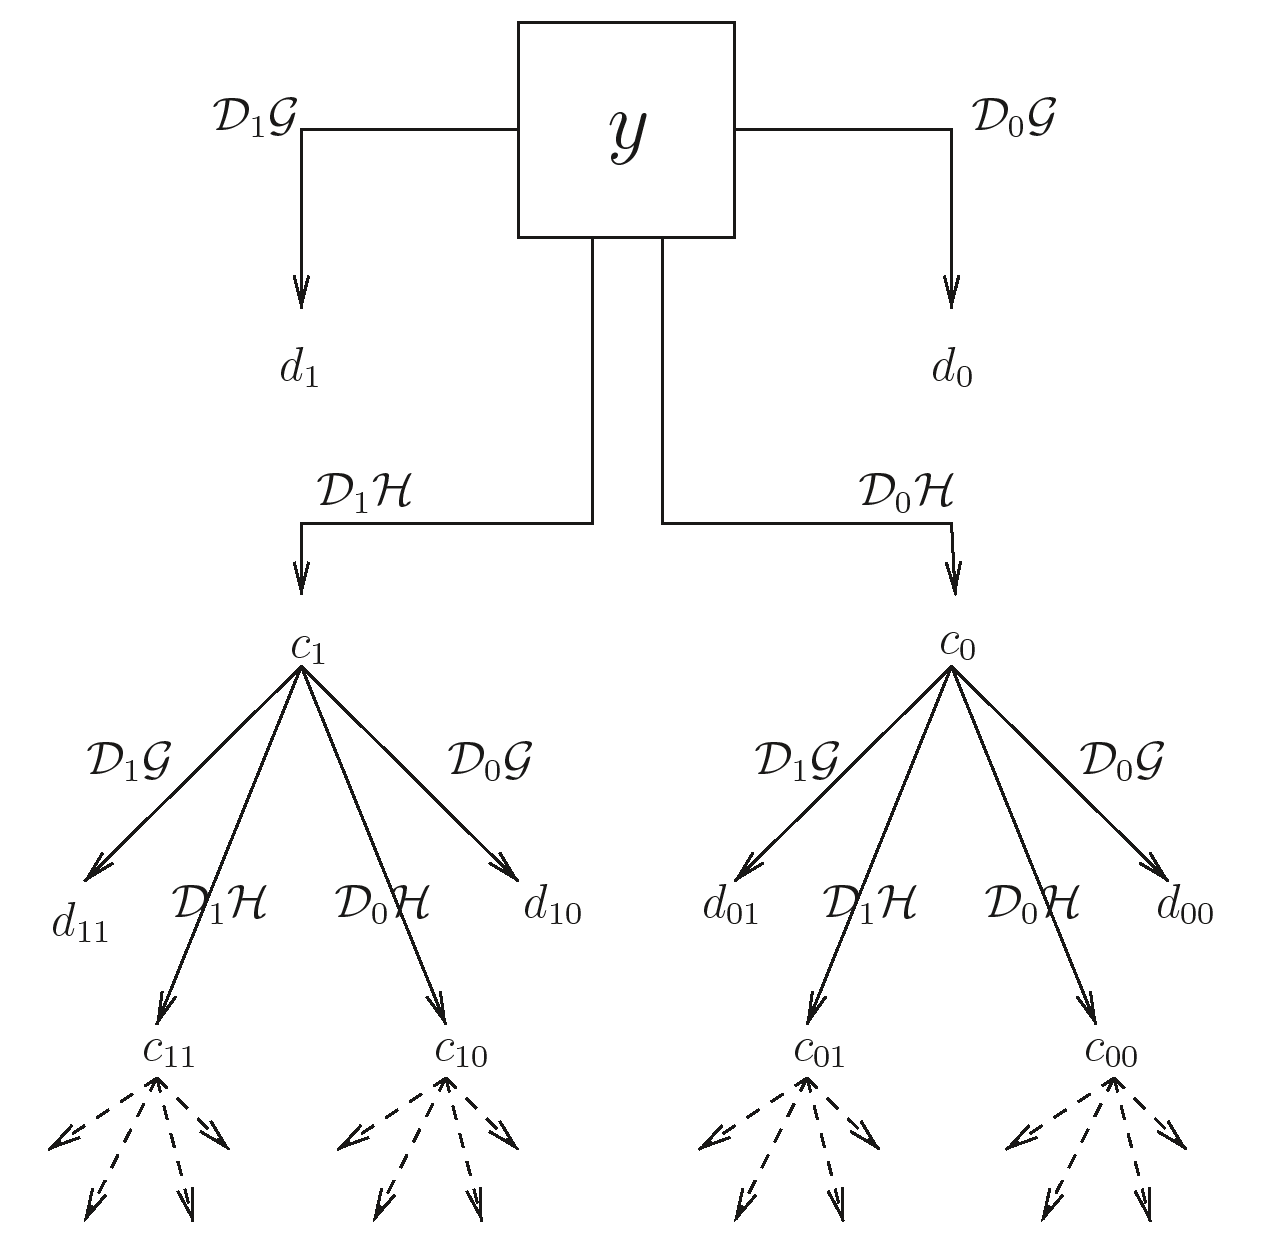
\includegraphics[width=17.58in]{images/advmultiscale_nondecimated} 

}

\caption{Non-decimated wavelet transform flow diagram.}\label{fig:unnamed-chunk-128}
\end{figure}

비-데시메이티드 웨이블릿 변환의 실행 절차는 다음과 같다.

\begin{enumerate}
\def\labelenumi{\arabic{enumi}.}
\item
  주어진 자료를 \(\mathcal{y}=(y_{1},\ldots ,y_{n})^{T}\)라고 하자.
  그러면 even and odd indexed `wavelet' filtered observations
  \[\mathbf{d}_{0}=\mathcal{D}_{0}\mathcal{G}\mathbf{y} \text{ and }\mathbf{d}_{1}=\mathcal{D}_{1}\mathcal{G}\mathbf{y}\]
  를 저장해 놓는다. 이 두 상세계수는 각각 \(\frac{n}{2}\)개로, 합치면
  \(n\)개가 되고 임의 레벨에서의 계수 숫자는 줄지 않는다.
\item
  \(\mathbf{c}_{0}=\mathcal{D}_{0}\mathcal{H}\mathbf{y}\),
  \(\mathbf{c}_{1}=\mathcal{D}_{1}\mathcal{H}\mathbf{y}\)를 계산한다.
  (역시 각각 \(\frac{n}{2}\)개다)
\item
  계속 반복한다. 즉
  \(\mathcal{D}_{0}\mathcal{G}, \mathcal{D}_{1}\mathcal{G}, \mathcal{D}_{0}\mathcal{H}, \mathcal{D}_{1}\mathcal{H}\)를
  \(\mathbf{c}_{0}\)와 \(\mathbf{c}_{1}\)에 적용한다. 자세한건 그림을
  참조하자. 참고로
  \(\mathbf{d}_{00}, \mathbf{d}_{01}, \mathbf{d}_{10}, \mathbf{d}_{11}\)은
  각각 \(\frac{n}{4}\)개만큼 있다.
\end{enumerate}

이러한 방법을 따라 계속하면, \(J-j\) scale에는 \(2^{j}\) set of 계수들이
존재하며 각각의 길이는 \(2^{-j}n, j=1,\ldots, J\)이다. (참고
\(n=2^{J}\)) 각 레벨에서의 웨이블릿 계수들의 수는
\(2^{-j}n\times s^{j}=n\)으로 항상 일정하다. 스케일이 \(J\)만큼 있으면
계수들의 총 수는 \(Jn\)이며, \(J=\log_{2}n\)이므로, 계수들의 총 수는
다시 \(n\log_{2}n\)으로 쓸 수 있다. 즉 NDWT를 위한 computational effort
또한 \(\mathcal{O}(n\log_{2}n)\)이다. 이는 DWT의 computation effort
\(\mathcal{O}_{n}\)보다는 느리나 그래도 빠른 편으로 생각할 수 있다.

우리는 종종 계수들의 set을 \textbf{패킷(packet)}으로 부르기도 한다.
그러나 이 패킷은 뒤에 나올 웨이블릿 패킷과는 다른 얘기다.

\subsection{시간순서 NDWT와 패킷순서 NDWT(time and packet NDWT
orderings)}\label{-ndwt--ndwttime-and-packet-ndwt-orderings}

다음과 같은 자료 \(\mathbf{y}=(y_{1}, \ldots , y_{8})\)이 있다고 하자.

\begin{itemize}
\tightlist
\item
  Time-ordered NDWT: 시간 순서에 따라 NDWT르 하는 것이다. 즉
\end{itemize}

\[(y_{2}-y_{1}), (y_{3}-y_{2}), (y_{4}-y_{3}), (y_{5}-y_{4}), (y_{6}-y_{5}), (y_{7}-y_{6}), (y_{8}-y_{7}), (y_{1}-y_{8})\]
이다. 이 방법은 시계열자료에 많이 사용한다.

\begin{itemize}
\tightlist
\item
  Packet-ordered NDWT: 패킷 두 개로 나누어 계산한다.
\end{itemize}

\[\mathcal{D}_{0}\mathcal{G}\text{관련: } (y_{2}-y_{1}), (y_{4}-y_{3}), (y_{6}-y_{5}), (y_{8}-y_{7})\]

\[\mathcal{D}_{1}\mathcal{G}\text{관련: } (y_{3}-y_{2}), (y_{5}-y_{4}), (y_{7}-y_{6}), (y_{1}-y_{8})\]

이 방법은 operator에 따라 함수의 특성을 잘 찾아내는 게 있으므로
함수자료에 좋다(ex.regression)

종합하면 두 방법은 같은 방법이다. 다만 순서가 다르다.

\section{R 예제(R-NDWT)}\label{r-r-ndwt}

데이터 \(\mathbf{y}=(1,1,7,9,2,8,8,6)\)이 있다고 하자. R 패키지
\texttt{wavethresh}에서 시간순서 DWT를 하려면 \texttt{wd} 함수에서
\texttt{type="station"}을 입력하면 된다.

(filter number와 family에 대한 설명 필요)

\begin{Shaded}
\begin{Highlighting}[]
\NormalTok{ywdS <-}\StringTok{ }\KeywordTok{wd}\NormalTok{(y, }\DataTypeTok{filter.number=}\DecValTok{1}\NormalTok{, }\DataTypeTok{family=}\StringTok{"DaubExPhase"}\NormalTok{, }\DataTypeTok{type=}\StringTok{"station"}\NormalTok{)}
\KeywordTok{accessD}\NormalTok{(ywdS, }\DataTypeTok{level=}\DecValTok{2}\NormalTok{) }\CommentTok{#finest-scale non-decimated wavelet coefficients(time-order)}
\end{Highlighting}
\end{Shaded}

\begin{verbatim}
> [1]  0.000000 -4.242641 -1.414214  4.949747 -4.242641  0.000000  1.414214
> [8]  3.535534
\end{verbatim}

이번에는 패킷순서 DWT이다. 이때는 \texttt{wd} 대신 \texttt{wst} 함수를
쓴다.

\begin{Shaded}
\begin{Highlighting}[]
\NormalTok{ywst <-}\StringTok{ }\KeywordTok{wst}\NormalTok{(y, }\DataTypeTok{filter.number=}\DecValTok{1}\NormalTok{, }\DataTypeTok{family=}\StringTok{"DaubExPhase"}\NormalTok{)}
\KeywordTok{accessD}\NormalTok{(ywst, }\DataTypeTok{level=}\DecValTok{2}\NormalTok{) }\CommentTok{#finest-scale non-decimated wavelet coefficients(packet-order)}
\end{Highlighting}
\end{Shaded}

\begin{verbatim}
> [1]  0.000000 -1.414214 -4.242641  1.414214 -4.242641  4.949747  0.000000
> [8]  3.535534
\end{verbatim}

이들 중 odd-decimated coefficient들만 뽑으려면 다음과 같이 하면 된다.

\begin{Shaded}
\begin{Highlighting}[]
\KeywordTok{getpacket}\NormalTok{(ywst, }\DataTypeTok{level=}\DecValTok{2}\NormalTok{, }\DataTypeTok{index=}\DecValTok{1}\NormalTok{)}
\end{Highlighting}
\end{Shaded}

\begin{verbatim}
> [1] -4.242641  4.949747  0.000000  3.535534
\end{verbatim}

\texttt{index}를 바꾸어 레벨을 바꿀 수 있다.

\begin{Shaded}
\begin{Highlighting}[]
\KeywordTok{getpacket}\NormalTok{(ywst, }\DataTypeTok{level=}\DecValTok{1}\NormalTok{, }\DataTypeTok{index=}\DecValTok{3}\NormalTok{)}
\end{Highlighting}
\end{Shaded}

\begin{verbatim}
> [1] -2.5 -0.5
\end{verbatim}

다음은 \texttt{ywst}로 얻은 계수들을 \texttt{ywd}타입으로 바꾸는
명령어다.

\begin{Shaded}
\begin{Highlighting}[]
\KeywordTok{accessD}\NormalTok{(}\KeywordTok{convert}\NormalTok{(ywst), }\DataTypeTok{level=}\DecValTok{2}\NormalTok{)}
\end{Highlighting}
\end{Shaded}

\begin{verbatim}
> [1]  0.000000 -4.242641 -1.414214  4.949747 -4.242641  0.000000  1.414214
> [8]  3.535534
\end{verbatim}

\subsection{chirp 신호 예제}\label{chirp--}

대칭 chirp 함수를 \[y(x)=\sin(\pi/x)\] 로 정의한다. 이 때
\(x=\epsilon ' +(-1,-1,+\delta,-1+2\delta, \ldots, 1-2\delta)\)이며
\(\epsilon ' =10^{-5}\)이며 \(\delta=1/512\)이다. 이 함수의 그림은
다음과 같다.

\begin{Shaded}
\begin{Highlighting}[]
\NormalTok{y <-}\StringTok{ }\KeywordTok{simchirp}\NormalTok{()}
\KeywordTok{plot}\NormalTok{(y, }\DataTypeTok{type=}\StringTok{'l'}\NormalTok{, }\DataTypeTok{xlab=}\StringTok{"Time"}\NormalTok{, }\DataTypeTok{ylab=}\StringTok{"Chirp value"}\NormalTok{)}
\end{Highlighting}
\end{Shaded}

\begin{figure}

{\centering 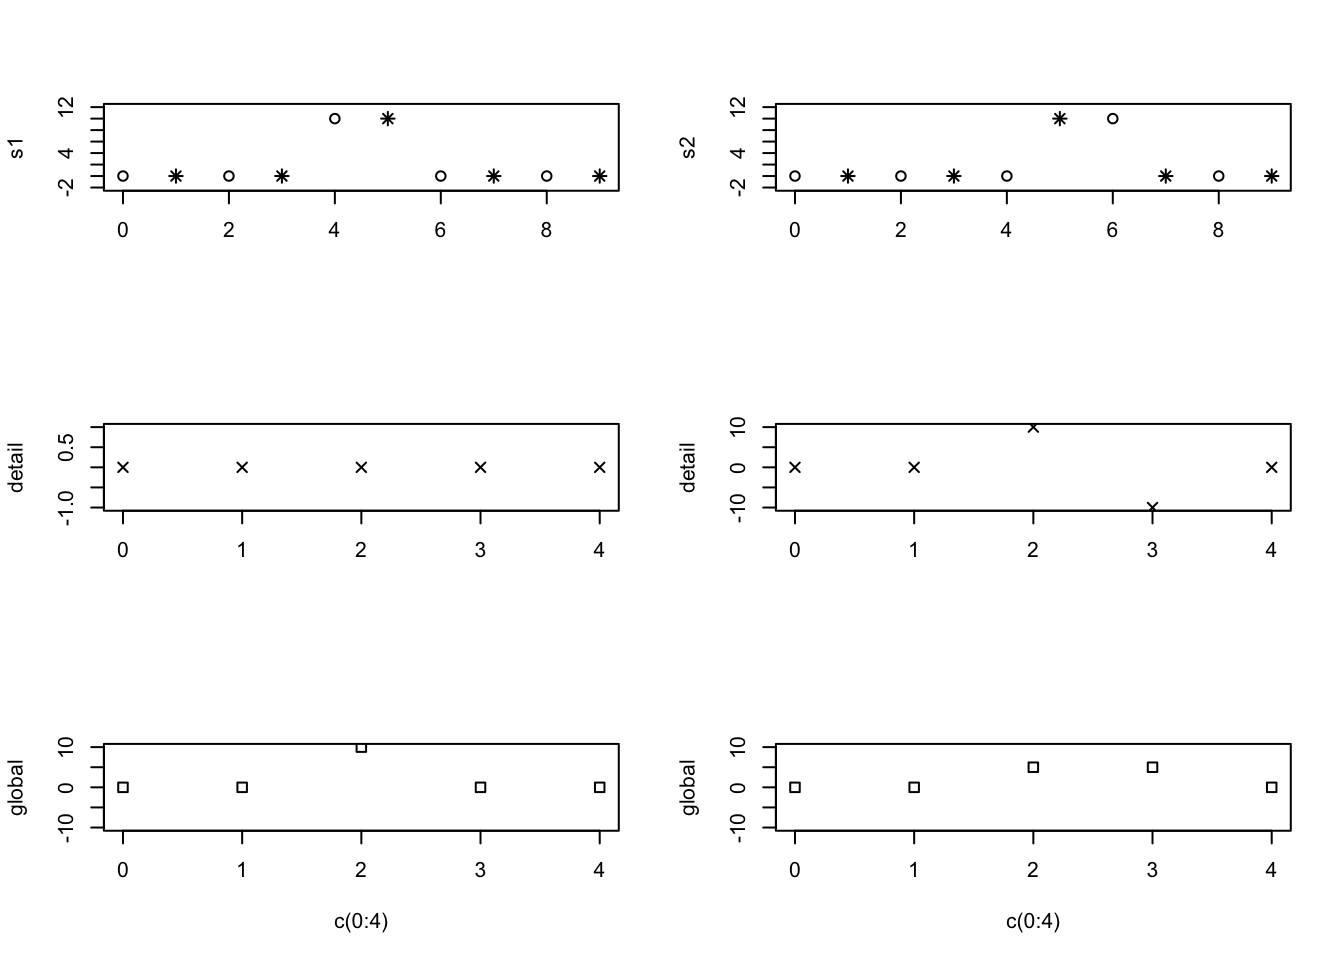
\includegraphics{book_files/figure-latex/unnamed-chunk-135-1} 

}

\caption{Simulated chirp signal.}\label{fig:unnamed-chunk-135}
\end{figure}

\begin{Shaded}
\begin{Highlighting}[]
\NormalTok{ywd <-}\StringTok{ }\KeywordTok{wd}\NormalTok{(y$y, }\DataTypeTok{filter.number=}\DecValTok{2}\NormalTok{, }\DataTypeTok{family=}\StringTok{"DaubExPhase"}\NormalTok{)}
\KeywordTok{plot}\NormalTok{(ywd, }\DataTypeTok{scaling=}\StringTok{"by.level"}\NormalTok{, }\DataTypeTok{main=}\StringTok{""}\NormalTok{)}
\end{Highlighting}
\end{Shaded}

\begin{figure}

{\centering 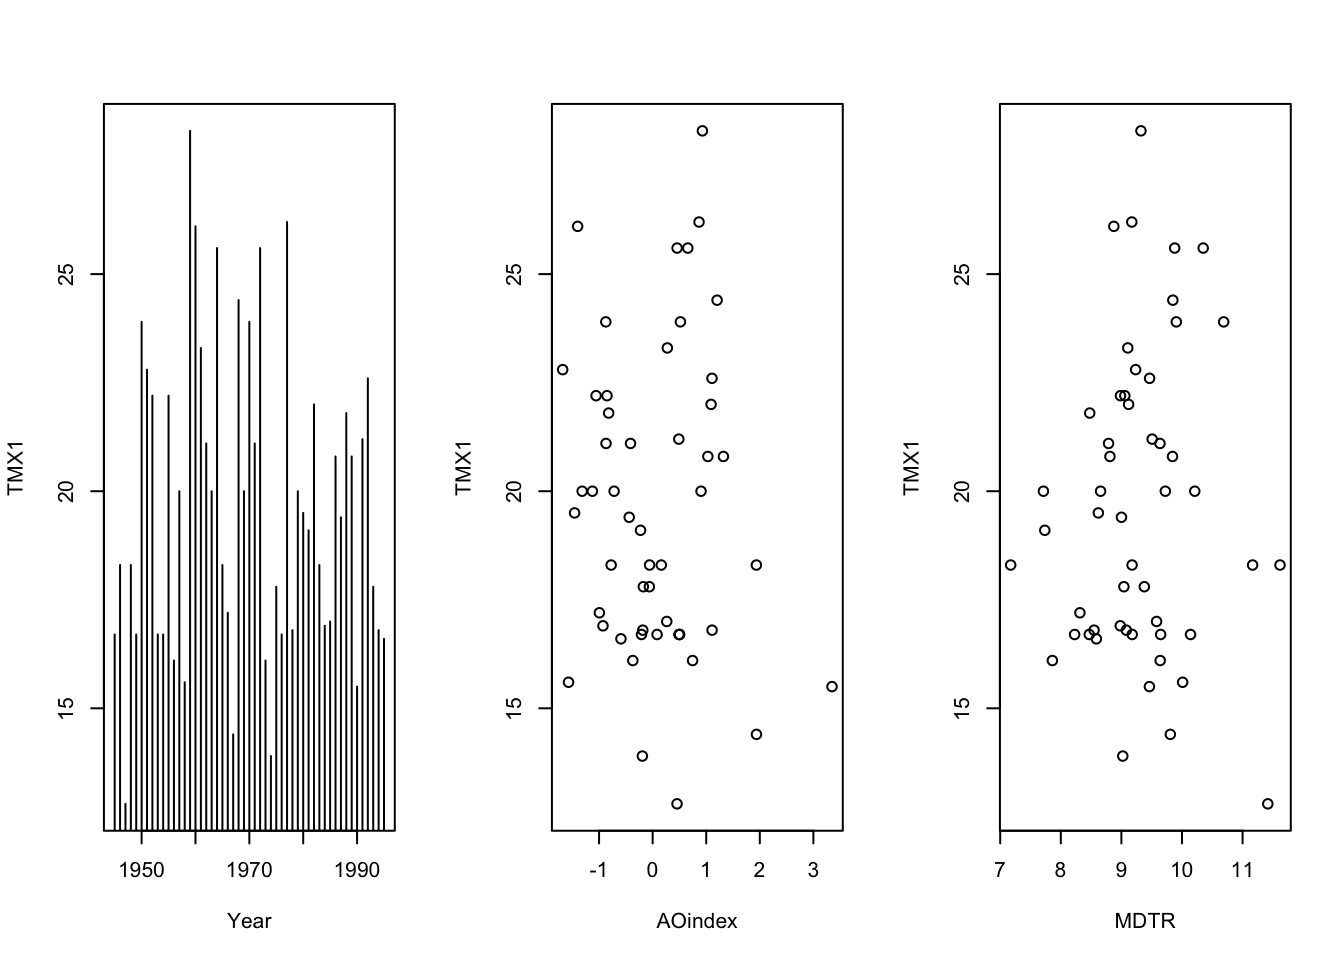
\includegraphics{book_files/figure-latex/unnamed-chunk-136-1} 

}

\caption{Discrete wavelet coefficients of simulated chirp signal.}\label{fig:unnamed-chunk-136}
\end{figure}

\begin{verbatim}
>  [1] 1.415688 1.704746 2.534105 3.084061 4.387454 5.564347 8.284556
>  [8] 7.484166 8.769223 4.756466
\end{verbatim}

\begin{Shaded}
\begin{Highlighting}[]
\NormalTok{ywd <-}\StringTok{ }\KeywordTok{wd}\NormalTok{(y$y, }\DataTypeTok{filter.number=}\DecValTok{2}\NormalTok{, }\DataTypeTok{family=}\StringTok{"DaubExPhase"}\NormalTok{, }\DataTypeTok{type=}\StringTok{"station"}\NormalTok{)}
\KeywordTok{plot}\NormalTok{(ywd, }\DataTypeTok{scaling=}\StringTok{"by.level"}\NormalTok{, }\DataTypeTok{main=}\StringTok{""}\NormalTok{)}
\end{Highlighting}
\end{Shaded}

\begin{figure}

{\centering 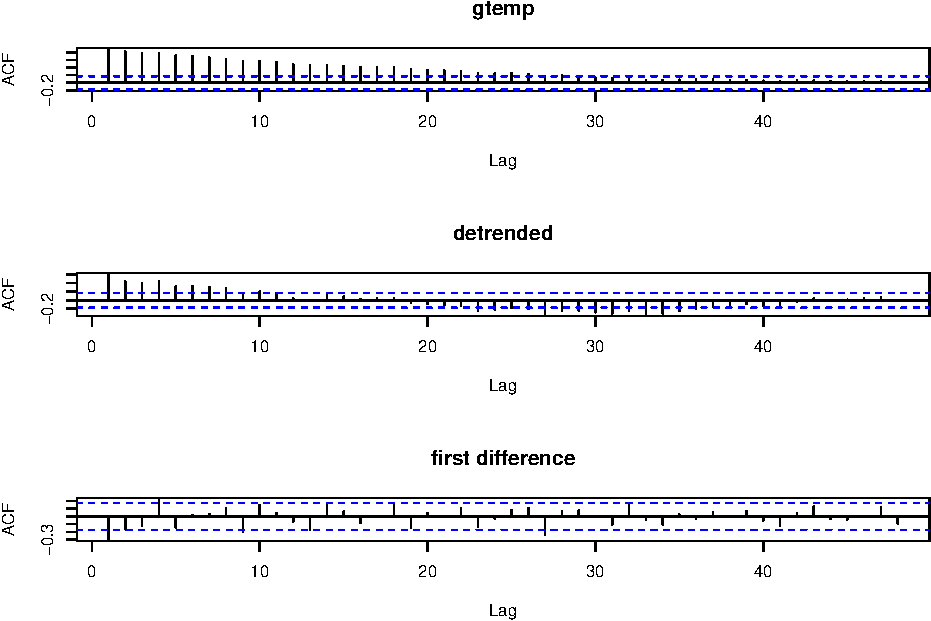
\includegraphics{book_files/figure-latex/unnamed-chunk-137-1} 

}

\caption{Time-ordered non-decimated wavelet coefficients of simulated chirp signal.}\label{fig:unnamed-chunk-137}
\end{figure}

\begin{verbatim}
>  [1]  1.570985  1.704746  2.534105  3.558442  5.030347  6.526141  8.756509
>  [8] 11.736733 13.175435  7.737538
\end{verbatim}

\begin{Shaded}
\begin{Highlighting}[]
\NormalTok{ywst <-}\StringTok{ }\KeywordTok{wst}\NormalTok{(y$y, }\DataTypeTok{filter.number=}\DecValTok{2}\NormalTok{, }\DataTypeTok{family=}\StringTok{"DaubExPhase"}\NormalTok{)}
\KeywordTok{plot}\NormalTok{(ywst, }\DataTypeTok{scaling=}\StringTok{"by.level"}\NormalTok{, }\DataTypeTok{main=}\StringTok{""}\NormalTok{)}
\end{Highlighting}
\end{Shaded}

\begin{figure}

{\centering 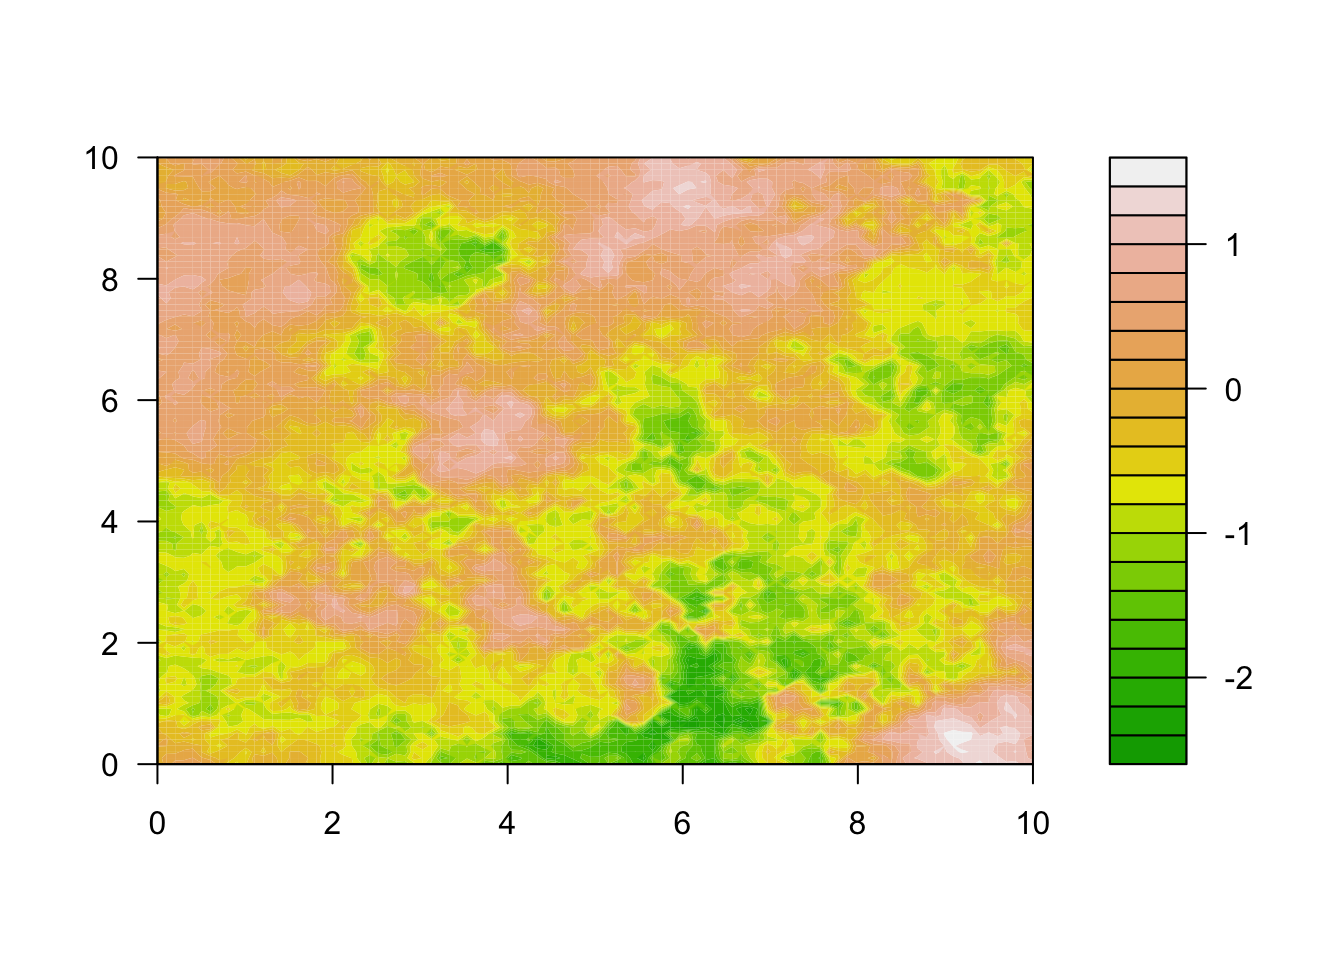
\includegraphics{book_files/figure-latex/unnamed-chunk-138-1} 

}

\caption{Packet-ordered non-decimated wavelet coefficients of simulated chirp signal.}\label{fig:unnamed-chunk-138}
\end{figure}

\section{Biorthogonal wavelet}\label{biorthogonal-wavelet}

이 내용은 \citep{Gomes2015}를 참고하였다. Orthogonality는 wavelet을
만드는 데 매우 큰 제약조건이다. 이것은 wavelet basis를 고르는 데 큰
제약을 준다. 예를 들면, Haar wavelet은 symmetric compact support를 갖는
유일한 orthogonal basis다. 웨이블릿 함수의 바람직한 조건들을
유지시키면서 좀 더 flexible한 선택을 위해 orthogonality를
biorthogonality로 바꾼다.

\subsection{Biorthogonal 기저 함수들(Biorthogonal basis
functions)}\label{biorthogonal--biorthogonal-basis-functions}

\begin{figure}

{\centering 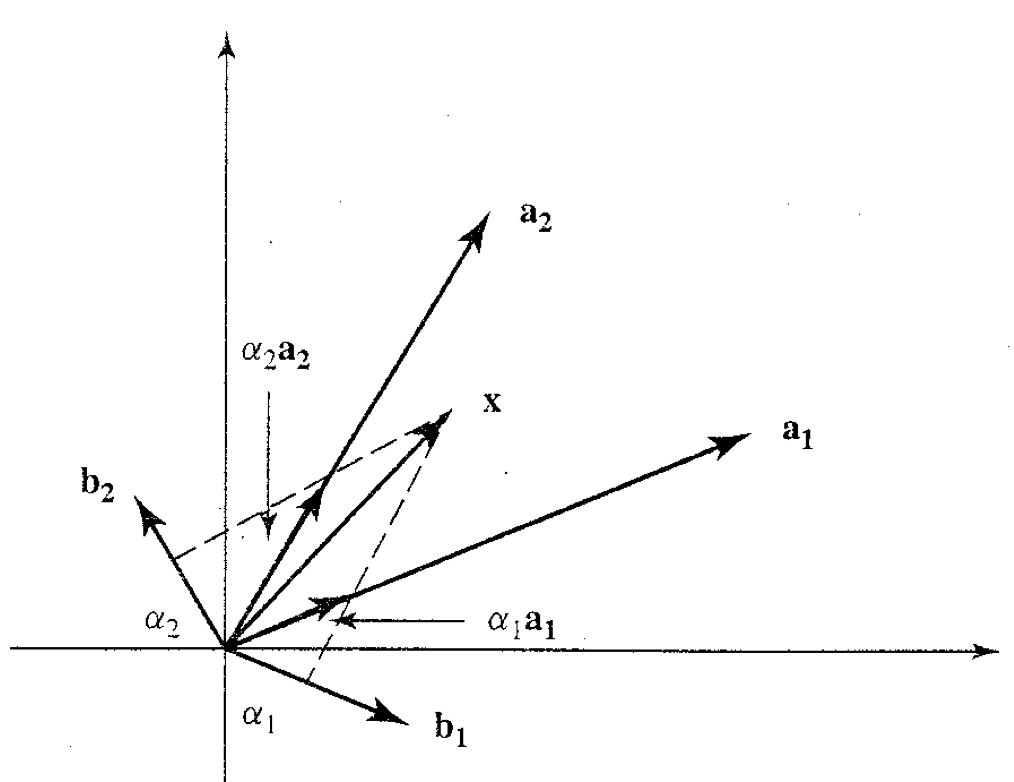
\includegraphics[width=14.08in]{images/multiscale_Dualbasis} 

}

\caption{Dual basis.}\label{fig:unnamed-chunk-139}
\end{figure}

\chapter{웨이블릿 수축}\label{waveletshrinkage}

이 장의 주된 내용과 그림들은 \citep{Nason2010}를 참고하였다.

다음과 같이 자료를 관찰하는 도메인(domain)인 physical domain (physical
model)에서의 모델 \(y_{i}=g(x_{i})+e_{i}, i=1,\cdots,n\)에서 관측한 길이
\(n\)의 자료 \(\mathbf{y}=(y_{1},\cdots,y_{n})^{T}\)이 있다고 하자.
여기서 \(x_{i}=\frac{i}{n} \text{ (designed point)}\)이라고 하자. 이
공간(space)은 equally-spaced이고 \(x \in (0, 1]\)이다. 우리의 목표는
알려지지 않은 함수 \(g(x), x \in [0,1]\)를 추정하는 것이다.

일반적으로 \(e_{i} \stackrel{iid}{\sim} \mathcal{N}(0,\sigma^{2})\)으로
가정한다. \textbf{독립 동일 분포 가정(independent and identically
distributed, iid)}이 없으면 모형이 좀 더 복잡해진다.
\textbf{정규분포(normal distribution, Gaussian distribution)} 가정도
중요한데, 정규분포처럼 대칭(symmetric)인 분포를 가정하지 않을 경우 평균
추정이 힘들어지므로 보통 \textbf{분위수(quantile)} 추정을 하게 된다.

우리가 얻는 자료 \(\mathbf{y}\)가 noise가 전혀 없는 순수한 signal이라고
하면, wavelet transform후 바로 wavelet reconstruction을 통해 원래 자료를
얻을 수 있다.
\[\mathbf{y} \xrightarrow{W} \boldsymbol{\delta} \xrightarrow{W^{-1}} \mathbf{y}\]
그런데 자료에 \textbf{잡음(noise)}이 있는 경우 얘기가 좀 달라진다.
\[\mathbf{d}=\mathbf{Wy} =\mathbf{Wg}+\mathbf{We}=\boldsymbol{\theta}+\boldsymbol{\epsilon}\]
이 경우에는 위와 같은 방법을 적용하면 잡음이 낀 신호가 그대로 나오게
된다. 우리는 적당한 방법을 통해 noise가 거의 없는 \(\hat{\mathbf{d}}\)를
추정해
\(\mathbf{W}^{-1}\hat{\mathbf{d}} \rightarrow \hat{\mathbf{g}}\)를 하고
싶다. 이럴 떄 쓰는 방법이 \textbf{임계화(thresholding)}이다.

\section{웨이블릿 수축의 주된 개념(main concept of wavelet
shrinkage)}\label{---main-concept-of-wavelet-shrinkage}

다시 원래 얘기로 돌아가서 우리는 웨이블릿 변환을 통해 \(g\)를 추정하고자
한다. \(\mathbf{W}\)를 이산 웨이블릿 변환 \textbf{연산자(연산자)}라고
하면, 다음과 같은 웨이블릿 변환을 생각해 볼 수 있다.

\[\mathbf{y}=\mathbf{g}+\mathbf{e} \rightarrow \mathbf{Wy} =\mathbf{Wg}+\mathbf{We} \text{ or } \mathbf{d}=\boldsymbol{\theta}+\boldsymbol{\epsilon}.\]

웨이블릿 변환 연산자는 physical domain에 있는 자료를 wavelet domain
(model in the wavelet domain, wavelet-transformed model or wavelet
model)으로 보내주는 역할을 한다. 웨이블릿 변환은
정규직교(orthonormal)이므로 변환된 오차항 또한
\(\epsilon \sim \mathcal{N}(0,\sigma^{2}\mathbf{I})\)로 정규분포를
따르는 좋은 성질을 가진다. 또 웨이블릿 변환은 오차(error(가 약하게
correlated (stationary process)된 경우 웨이블릿 변환을 하면 변환된
오차가 de-correlated(whitening, 더 약하게 correlated되는 것)되는 좋은
성질이 있다.

\textbf{웨이블릿 수축(wavelet shrinkage)}을 위해 알아두어야 할 컨셉들은
다음과 같다.

\begin{itemize}
\item
  \(\boldsymbol{\theta}\)는 많은 함수들의 \textbf{성긴 벡터(sparse
  vector)}이다. 그리고 \(\boldsymbol{\theta}\)는 다음과 같이 Parseval's
  identity를 만족시킨다. 즉 데이터의 에너지와 계수들의 에너지가
  같다(보존된다). \[\sum g^{2}(x)=\sum \theta_{i}^{2}.\]
\item
  \(\boldsymbol{\theta}\)는 ``concentrated''되어있다.
\item
  \(\epsilon \sim \mathcal{N}(0,\sigma^{2}\mathbf{I})\), 즉 웨이블릿
  계수 \(\mathbf{d}\)에는 \(\boldsymbol{\theta}\)뿐 아니라
  \(\mathbf{\epsilon}\)의 정보도 들어있다.
\item
  위의 사실에 기초하여 \(\mathbf{d}\)중 값이 큰 원소의 경우에는 진짜
  신호 + 잡음의 형태로 이루어져 있을 것이다.
\item
  \(\mathbf{d}\)중 값이 작은 원소의 경우에는 잡음만 있을 것이다.
\end{itemize}

이런 상황에서는 평균이 틀리게 된다. 즉
\(\hat{\theta}=\frac{1}{n}\sum_{i=1}^{n}d_{i}\)가 \(\theta\)의 좋은
추정량이 될 수 없다는 것이다. 그래서 이를 해결하기 위해 도입된
아이디어가 \textbf{임계화(thresholding)}이다. 임계화가 등장하기 전까지
모든 추정량에는 평균 개념이 있었다. (ex. Ridge) 기존의 자료분석들은
``aggregation''에 치중했다. 모든 변수에 다 신호가 존재한다고 생각한
것이다. 이런 방식으로는 위의 문제를 해결할 수 없다. 그러나 웨이블릿
변환의 등장 이후에는 ``sparsity'' 개념이 등장하였고 몇 개의 신호만
선택하게 되었다. 이 개념 덕분 에 고차원(high-dimensional)
자료(\(n \ll p\))를 분석할 수 있게 되었다.

수축 방법에는 두 가지가 있다. \textbf{하드 임계화(hard thresholding)}와
\textbf{소프트 임계화(soft thresholding)}가 그것이다. 두 임계화를 다음과
같이 정의한다.

\BeginKnitrBlock{definition}[하드 임계화와 소프트 임계화]
\protect\hypertarget{def:unnamed-chunk-140}{}{\label{def:unnamed-chunk-140}
\iffalse (하드 임계화와 소프트 임계화) \fi{} }주어진 (empirical)
웨이블릿 상수 d와 \textbf{threshold} \(\mathbf{\lambda}\)가 있을 때,
그것의 \textbf{하드 임계화(hard thresholding)}는
\[\hat{\theta}_{H}=\eta_{H}(d,\lambda)=d\mathbb{I}\{ |d| > \lambda \}\]
이다. 그리고 \textbf{소프트 임계화(soft thresholding)}는
\[\hat{\theta}_{S}=\eta_{S}(d,\lambda)=\text{sgn}(d)(|d|-\lambda)\mathbb{I}\{ |d| > \lambda \}\]
이다.
\EndKnitrBlock{definition}

\begin{figure}

{\centering 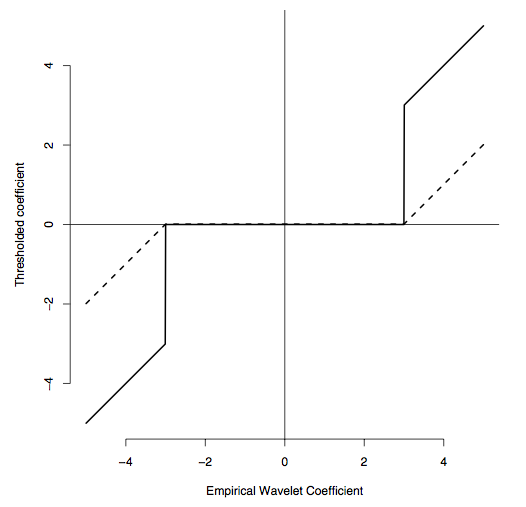
\includegraphics[width=7.31in]{images/waveletshrinkage_thresholding} 

}

\caption{Hard thresholding (dotted line) and soft thresholding.}\label{fig:unnamed-chunk-141}
\end{figure}

두 방법 다 공통적으로 \(\mathbf{d} \in (-\lambda, \lambda)^{n}\)이면 0이
된다.

하드 임계화는 ``keep or kill'' 방법이라고도 불린다. 그 이유는 값이 어떤
threshold(\(\mathbf{\lambda}\))보다 작을 경우 무조건 0으로 놓기
때문이다. 이것은 회귀분석의 변수 선택(variable selection)과 동일한
아이디어이다. 변수 선택에서도 변수를 넣기 또는 빼기 두 가지 선택지만
있다는 것을 생각하기 바란다. 그리고 하드임계화에서는 축소를 하지 않는다.
소프트 임계화는 하드 임계화를 함과 동시에 신호 변환 함수가 연속이 되도록
값이 큰 signal도 같이 축소(shrinkage)하는 방법이다. 이는 변수선택에서
LASSO와 대응되는 방법이다.

때때로 굉장히 큰 \(\mathbf{d}\)에는 오차가 작게 들어있을 것이라 생각할
수도 있다. 이를 보완하기 위해 SCAD 같은 방법들이 나중에 제안되었는데,
원래 이는 웨이블릿을 연구하는 학자들이 생각했던 개념으로 이를 통계학
언어로 옮긴 것에 불과하다.

여기서 등장하는 \(\lambda\)는 \textbf{핵평활(kernel smoothing)}이나
\textbf{평활 스플라인(smoothing spline)}에서 나오는
\textbf{띠너비(bandwidth)}와 비슷한 개념이라고 생각하면 된다.
\(\lambda\)의 선택 또한 중요한 이슈가 된다. 이것을 어떻게 선택하느냐에
따라 performance가 굉장히 변하고 \(\hat{g}\)의 질(quality)에 영향을
미친다.
\[y \xrightarrow{W} d \xrightarrow{\text{th}} \hat{\theta}_{Shrink} \xrightarrow{W^{-1}} \hat{g}.\]

\section{오라클(oracle)}\label{oracle}

만약 우리가 \(g\)를 알고 있다면, \(\hat{g}\)의 quality를 계산하는 방법
중 하나로 다음과 같은 \textbf{적분제곱오차(integrated squared error,
ISE, \(\hat{M}\))}를 생각해 볼 수 있다.

\[\hat{M}=\frac{1}{n}\sum_{i=1}^{n}(\hat{g}(x_{i})-g(x_{i}))^{2}.\]
그러나 우리는 \(g\)를 모르기 때문에 실제로 ISE를 계산할 수는 없다. 대신
`평균(average)' 개념을 적용한 \textbf{평균적분제곱오차(mean integrated
squared err, MISE)} \(E(\hat{M})\)을 정의한다.

\[ M \triangleq E(\hat{M})=\text{Risk of }\hat{g}.\] 웨이블릿에서
\(\hat{g}\)는 \(\lambda, \eta, \theta\)에 좌우(depend)한다. 참고로 보통
\(g\)가 정의되는 함수공간 \(g \in \mathcal{F}\)은 일반적으로
\(L^{2}(\mathbb{R})\)에서만 생각한다. 웨이블릿은 점프가 있는 함수도 다룰
수 있긴 하다. 결국 통계적 추정의 목표는 이 MISE를 최소화하는
\(\hat{g}\)를 찾는 것이다.

웨이블릿에서
\(\hat{M}=\sum_{j,k}(\hat{\theta}_{jk}-\theta_{jk})^{2}\)이다. 여기서
웨이블릿 변환은 정규직교이므로 'decoupling'이라는 성질을 이용할 수 있다.
이 얘기는 위의 값을 계산할 때 \(j,k\)를 무시하고 마치 하나만 있는 것처럼
계산해도 된다는 것이다. 마치 벡터(vector)를 스칼라(scalar)처럼 볼 수
있다는 것이다.

잠시 선형 회귀분석 모형을 복습해보자. 다음과 같은 선형 회귀분석 모형
\[\mathbf{y}=\mathbf{X}\boldsymbol{\beta}+\boldsymbol{\epsilon}\] 이
있다고 하자. 여기서 \(\mathbf{y}\)는 \(n \times 1\) 행렬,
\(\mathbf{X}\)는 \(n \times d\) 행렬, \(\boldsymbol{\beta}\)는
\(d \times 1\) 행렬, 그리고 \(\boldsymbol{\epsilon}\)은 \(n \times 1\)
행렬이다. 만약 여기서 \(X\)의 열(column)이 정규직교라고 해보자. 그러면

\begin{eqnarray*}
\hat{\boldsymbol{\beta}}&=&(\hat{\beta}_{1},\cdots,\beta_{d})^{T}=(\mathbf{X}^{T}\mathbf{X})^{-1}\mathbf{X}^{T}\mathbf{y}=\mathbf{X}^{T}\mathbf{y}\\
&\Longrightarrow& \hat{\beta}_{1}=\sum X_{i1}y_{i}, \hat{\beta}_{2}=\sum X_{i2}y_{i}, \cdots
\end{eqnarray*}

로 모든 \(\boldsymbol{\beta}\)의 원소들이 separate(decoupled)되는 것을
볼 수 있다. 참고로 \((\mathbf{X}^{T}\mathbf{X})^{-1}\neq \mathbf{I}\)인
경우 \(\hat{\beta}\)가 다 연결되므로 이렇게 분석할 수 없다. 그리고
\[\hat{\boldsymbol{\beta}}=\min \| \mathbf{y}-\mathbf{X}\boldsymbol{\beta} \|^{2} \Leftrightarrow \min \| \mathbf{X}^{T}\mathbf{y} - \mathbf{X}^{T}\boldsymbol{\beta} \|^{2}=\min \| \hat{\boldsymbol{\beta}}-\boldsymbol{\beta} \|^{2}\]
가 된다. \citep{Donoho1994} 논문에 갑자기 이 사실을 이용해 전개하는
내용이 있다.

더 나아가 벌점화 최소자승법(penalized least square) 문제를 생각해보자.
\(\mathbf{z}=\mathbf{X}^{T}\mathbf{y}\),
\(\hat{\mathbf{y}}=\mathbf{Xz}=\mathbf{XX}^{T}\mathbf{y}\)를 정의하면

\begin{eqnarray*}
\| \mathbf{y}-\mathbf{X}\boldsymbol{\beta}\|^{2}+\lambda \sum_{j=1}^{d}P(| \beta_{j} |) &=& \| \mathbf{y}-\hat{\mathbf{y}}+\hat{\mathbf{y}}-\mathbf{X}\boldsymbol{\beta}\|^{2}+\lambda \sum_{j=1}^{d}P(|\beta_{j}|)\\
&=&\| \mathbf{y} -\hat{\mathbf{y}} \|^{2} + \sum_{j}(z-{j}-\beta_{j})^{2}=\lambda\sum_{j}P(|\beta_{j}|)\\
\end{eqnarray*}

여기서 \(\| \mathbf{y} -\hat{\mathbf{y}} \|^{2}\)는 \(\beta_{j}\)와 관련
없으므로 뒤의 두 항만 최소화(minimize)하면 된다. 그런데 \(\beta_{j}\)는
seperate되므로 벌점화 최소자승법의 해는
\[\hat{\beta}=\min_{\beta}(z-\beta)^{2}+\lambda P(| \beta |)\] 이다.

다시 웨이블릿 문제로 돌아가서, 웨이블릿 변환 행렬 \(\mathbf{W}\)
(회귀분석에서 \(\mathbf{X}\)와 같은 역할을 함)이 정규직교이므로, 우리는
\(E(\hat{\theta}-\theta)^{2}\)(=risk)만 보면 된다. 참고로
\(\mathbf{W}\)는 정방행렬(square matrix)이라는 점에서 \(\mathbf{X}\)와
다르다. Separated 성질에 의해

\[
M(\hat{\theta},\theta)=E(\hat{\theta}-\theta)^{2} =
\begin{cases}
E(d-\theta)^{2}=E\epsilon^{2} & \text{if $|d| > \lambda$}\\
E(\theta^{2})=\theta^{2} & \text{o.w.}
\end{cases}
\] 이 된다. 결론적으로 임계화(thresholding)를 위해서는 신호와 오차의
크기를 비교해 보면 되는데, 만약 신호가 오차보다 굉장히 큰 경우,
\(\theta \gg \sigma\)인 경우면 우리는 \(|d| > \lambda\)인 경우를
취하는게 유리하므로 \(\lambda\)를 작게 선택하면 된다. 반대의 경우에는
\(\lambda\)를 크게 취하는 것이 유리하다.

통계학에서 오라클이라는 개념을 처음 사용한 사람은 Dave Donoho이다.
오라클이라는 개념이 처음 등장하는 논문은 \citep{Donoho1994}인데,
오라클을``With ideal spatial adaptation, an oracle furnishes information
about how best to adapt a spatially variable estimator, whether
piecewise constant, piecewise polynomial, variable knot spline, or
variable bandwidth kernel to the unknown function''이라고 소개하고 있다.
교수님의 요약은 다음과 같다. ``The oracle is notional device that tells
you which coefficients you should select.''

오라클에 의한 ideal risk는(hard thresholding의 경우)
\(M_{ideal}=\sum_{j,k}\min(\theta_{j,k}^{2},\sigma^{2})\)이다. 그렇다면
\(\hat{\theta}\)를 어떻게 구하는가? 이 문제는 결국
\(\eta_{H}, \eta_{S}, \lambda\)를 선택하는 문제로 귀착된다. Donoho와
Johnstone은 \(M_{ideal}\approx M\)이 되게 하는 \(\hat{\theta}\)를 몇
가지 제시하였다. \citep{Donoho1994}에서
\(\hat{\theta}=\eta_{x}(d,\lambda)\),
\(\lambda=\sigma\sqrt{2\log n}\)으로 할 시
\[M_{\text{universal}}\leq(2\log n +1)(\sigma^{2}+M_{\text{ideal}})\]
임을 증명하였다. 다시 말하면 이 \(\hat{\theta}\)가 오라클 성질(oracle
property)과 굉장히 유사하며 \(M_{\text{ideal}}\)에
가깝게(대략\(2\log n\)배 보다 작다) 행동한다는 것이다. 위 논문에 따르면
핵평활(kernel smoothing)이나 평활 스플라인(smoothing spline)도
\(2\log n\)을 만족하지 못한다(n). 가장 이상적인 fitting은 정확한 knot
point들을 모두 알고 있는 piecewise polynomial이다. 그러나 ideal한 knot을
모두 안다는 것은 true을 안다는 것이므로 이는 불가능하다. Bandwidth나
knot selection을 잘 한다는 것은 true의 분산을 안다는 것과 거의 같은
얘기다.

\section{만능 임계화(universal
thresholding)}\label{-universal-thresholding}

앞서 등장한 \(\lambda^{u}=\sigma \sqrt{2 \log n}\)을 특별히 \textbf{만능
임계화(universal Thresholding)}라고 한다. 실제로는 \(\sigma\)를 모르므로
\(\hat{\sigma}\)를 사용한다.

\BeginKnitrBlock{theorem}[만능 임계화]
\protect\hypertarget{thm:unnamed-chunk-142}{}{\label{thm:unnamed-chunk-142}
\iffalse (만능 임계화) \fi{} }\(X_{1},\cdots , X_{n}\)을
\(EX_{i}=0, EX_{i}^{2}=1, EX_{i}X_{i+k}=\gamma(k)\)인 stationary
Gaussian process (Lag-k covariance structure를 갖는 Gaussian
process)라고 하고 특별히 \(X_{(n)}=\max \{ X_{i} \}\)라 하자. 만약
\(\lim_{k \rightarrow \infty} \gamma (k) =0\)이면,
\[\frac{X_{(n)}}{\sqrt{2 \log n}} \rightarrow 1 \text{ as } n \rightarrow \infty\]
이다.
\EndKnitrBlock{theorem}

위 정리는 n Gaussian 확률 변수들 중 가장 큰 것은(독립일 필요는 없다)
대략 \(\sqrt{2 \log n}\) 사이즈라는 것이다. 이 정리에 비추어 만능
임계화를 생각하면 이 임계화는 오차(error)가 Gaussian random variable을
따르는 것이라면 모두 다 임계화하겠다는 뜻으로 해석할 수 있다. 이 방법은
이론적으로는 완벽해 보이기는 하나 너무나 많은 잡음(noise)을 줄이는
underfit한 임계화이다. 결국 SURE와 같은 실용적인 임계화 방법을 생각하게
된 것이다. 이 얘기는 추후에 다시 나올 것이다.

만능 임계화로 돌아가서, 우리는 \(\sigma\)를 모르므로 대신
\(\hat{\lambda}^{u}=\hat{\sigma}\sqrt{2 \log n}\)을 이용해야 할 것이다.
그렇다면 \(\sigma\)를 어떻게 추정할 것인가? 대부분의 방법은 data를
제외한 가장 finest scale (ex.J-1)의 detail 웨이블릿 계수(\(d_{J-1}\))를
이용해 추정한다. \(y\)를 이용해 \(\epsilon\)의 분산을 추정하려고 할 경우
\(f\)의 정보가 너무 강해서 \(\epsilon\)의 분산구조를 알 수 없을 것이다.
그리고 좀 더 성긴 스케일(coarser scale)로 갈수록 잡음보다는 신호 정보가
많을 것이라는 생각을 하면, \(d_{J-1}\)를 이용해 분산 구조를 추정하는
것이 당연하다.

가장 널리 알려진 방법은
\[\hat{\sigma}=\sqrt{\frac{1}{n/2-1}\sum_{k=1}^{n/2}(d_{J-1,k}-\bar{d_{J-1}})^{2}}\]
이다. 이 방법은 자료가 희소(sparse)한 경우에는 잘 맞지 않음이 알려져
있다. 그런 경우에는 대신 중앙값(median)을 이용하여 \[
\hat{\sigma}=1.4826 \times \text{median}(|d_{J-1,1}-\tilde{d_{J-1}}|,\cdots,|d_{J-1,\frac{n}{2}}-\tilde{d_{J-1}}|\\
\text{ where } \tilde{d}_{J-1}=\text{median}(\mathbf{d}_{J-1})
\] 이런 식으로 추정하기도 한다.

지금까지 했던 방법은 universal threshold rule(\(\lambda^{u}\))에 soft
thresholding function \(\eta_{s}\)를 적용한
\(\hat{\theta}=\eta_{s}(d,\lambda^{u})\)로 이것을
\textbf{VisuShrink}라고 부른다. 이 방법은 앞서 말한 대로 noise-free
reconstrunction이나 oversmooth (underfit)하는 문제가 생긴다. 즉
noise-free하지만 signal도 너무 많이 죽일 가능성이 있다는 것이다. 한편
\(\lambda^{u}\)는 noise-free reconstruction을 하는 최소의
\(\lambda\)이므로, \(0< \lambda^{*} \ll \lambda^{u}\)인
\(\lambda^{*}\)를 생각할 수 있을 것이다. 이런 \(\lambda^{*}\) 중의
하나로 \citep{Donoho1994}에서는 \textbf{RiskShrink}라는 것을 제시했다.
이 방법은 \(\Lambda_{n}^{*}(=2 \log n +1)\)에 해당하는
\(\Lambda_{n}^{*}\)과 이에 대응되는 \(\lambda^{*}\)을 table 형태로
계산한 것이다. 예를 들어 \(n=1024\) 일 때
\(\lambda^{u}=3.72, \lambda^{*}=2.23, \Lambda_{n}^{*}=5.976\)이다.

참고로 이 논문의 결과와 더불어 일반적으로 알려져 있는 사실은 함수가
부드럽(smooth)지 않을 때 웨이블릿이 다른 어떤 비모수 방법들보다 좋다는
것이다.

\section{Stein의 불편 위험 추정량(Steins Unbiased Risk Estimator
(SURE))}\label{stein---steins-unbiased-risk-estimator-sure}

앞서 얘기했던 VisuShirnk나 RiskShrink는 이론상으로는 완벽하나 실용성이
떨어져 실제로는 많이 쓰이지 않고 있다. 실제로 많이 쓰이는 shrinkage 방법
중 하나가 \textbf{Steins Unbiased Risk Estimator (SURE)}이다. Shrinkage
추정량들은 Bayesian과 밀접한 관련이 있다. Bayesian들이 주로 하는 것은
자료를 prior의 정보에 민감하게 반응하도록 수축(shrinkage)해 주는 것이다.

SURE가 처음 등장한 논문은 \citep{Donoho1995}로, \citep{Stein1981}의
내용을 웨이블릿 도메인으로 갖고 온 것이다. 다음과 같은 data domain에서의
모델
\(y_{i}=g(x_{i})+e_{i}, i=1,\cdots,n,e_{i} \stackrel{iid}{\sim} \mathcal{N}(0,\sigma^{2})\)과
이를 웨이블릿 도메인(domain)으로 옮긴
\(\mathbf{d}=\boldsymbol{\theta}+\boldsymbol{\epsilon}, \boldsymbol{\epsilon} \sim \mathcal{N}(0,\sigma^{2}\mathbf{I})\)를
생각하자. Stein의 논문에서는 이 notation을 다음과 같이 썼다.
\[\mathbf{x}=\boldsymbol{\mu}+\boldsymbol{\epsilon}.\]

\BeginKnitrBlock{theorem}[Stein]
\protect\hypertarget{thm:unnamed-chunk-143}{}{\label{thm:unnamed-chunk-143}
\iffalse (Stein) \fi{} }\citep{Stein1981} 만약
\(\hat{\boldsymbol{\mu}}\mathbf{(x)}=\mathbf{x}+\mathbf{g(x)}\),
\(g:\mathbb{R}^{n} \rightarrow \mathbb{R}^{n}\) is weakly differentiable
조건이면
\[E \| \hat{\boldsymbol{\mu}}\mathbf{(x)}-\boldsymbol{\mu} \|^{2} =n+ E\{ \|\mathbf{g(x)}\|^{2}+2\bigtriangledown \cdot \mathbf{g(x)} \}, \bigtriangledown\cdot \mathbf{g}=\sum_{i} \frac{\partial}{\partial x_{i}}g_{i}\]
이다.
\EndKnitrBlock{theorem}

그리고
\(\hat{\mu}_{i}(\lambda)=\eta_{s}(x_{i},\lambda) \Rightarrow \frac{\partial}{\partial x_{i}}\hat{\mu}_{i}(\lambda)=I( |x_{i}|>\lambda)\)과
\(\| \mathbf{g(x)} \|^{2}=\sum \hat{\mu}_{i}(\lambda, x)^{2}=\sum_{i=1}^{n}(|x_{i}|-\lambda)^{2}I(|x_{i}>\lambda)\)
사실을 이용해 SURE를 정의한다.

\BeginKnitrBlock{theorem}[SURE]
\protect\hypertarget{thm:unnamed-chunk-144}{}{\label{thm:unnamed-chunk-144}
\iffalse (SURE) \fi{}
}\(\text{SURE}(\lambda,\mathbf{x})=n-2\#\{ i: |x_{i}| \leq \lambda \} + \sum_{i=1}^{n}(|x_{i}| \wedge \lambda)^{2}\)는
risk의 불편추정량이다.
\[E \| \eta_{s}(\mathbf{x},\lambda)-\mu \|^{2}=E\text{SURE}(\lambda, \mathbf{x}).\]
실제로,
\(\lambda=\text{argmin}_{0<\lambda \leq lambda^{u}}\text{SURE}(\lambda,\mathbf{x})\)이며,
이 방법을 \textbf{SUREShrink}라고 한다.
\EndKnitrBlock{theorem}

\section{R 예제(R-waveletshrinkage)}\label{r-r-waveletshrinkage}

다음은 R 패키지 \texttt{wavethresh}를 이용한 축소 예제이다. 임계화를
위해 \texttt{threshold}라는 함수를 사용하며 \texttt{type} 및
\texttt{policy}를 선택할 수 있다.

\begin{Shaded}
\begin{Highlighting}[]
\KeywordTok{par}\NormalTok{(}\DataTypeTok{mfrow=}\KeywordTok{c}\NormalTok{(}\DecValTok{1}\NormalTok{,}\DecValTok{3}\NormalTok{))}
\KeywordTok{set.seed}\NormalTok{(}\DecValTok{1234}\NormalTok{)}
\NormalTok{data_bump <-}\StringTok{ }\KeywordTok{example.1}\NormalTok{()}
\NormalTok{x <-}\StringTok{ }\NormalTok{data_bump$x; y <-}\StringTok{ }\NormalTok{data_bump$y}
\KeywordTok{plot}\NormalTok{(x,y, }\DataTypeTok{type=}\StringTok{'l'}\NormalTok{, }\DataTypeTok{main=}\StringTok{"Original"}\NormalTok{)}
\NormalTok{y_noise <-}\StringTok{ }\NormalTok{y +}\StringTok{ }\KeywordTok{rnorm}\NormalTok{(}\KeywordTok{length}\NormalTok{(y), }\DataTypeTok{sd=}\FloatTok{0.1}\NormalTok{)}
\KeywordTok{plot}\NormalTok{(x,y_noise, }\DataTypeTok{type=}\StringTok{'l'}\NormalTok{, }\DataTypeTok{main=}\StringTok{"Noisy"}\NormalTok{)}
\NormalTok{y_noise_wd <-}\StringTok{ }\NormalTok{wavethresh::}\KeywordTok{wd}\NormalTok{(y_noise)}
\NormalTok{y_noise_threshold <-}\StringTok{ }\NormalTok{wavethresh::}\KeywordTok{threshold}\NormalTok{(y_noise_wd, }\DataTypeTok{type=}\StringTok{"soft"}\NormalTok{, }\DataTypeTok{policy=}\StringTok{"sure"}\NormalTok{)}
\NormalTok{y_sure <-}\StringTok{ }\NormalTok{wavethresh::}\KeywordTok{wr}\NormalTok{(y_noise_threshold)}
\KeywordTok{plot}\NormalTok{(x,y_sure, }\DataTypeTok{type=}\StringTok{'l'}\NormalTok{, }\DataTypeTok{main=}\StringTok{"Soft Thresholding"}\NormalTok{)}
\end{Highlighting}
\end{Shaded}

\begin{figure}

{\centering \includegraphics{book_files/figure-latex/unnamed-chunk-146-1} 

}

\caption{Wavelet shrinkage example.}\label{fig:unnamed-chunk-146}
\end{figure}

\chapter{웨이블릿 수축의 고등 논제들}\label{advwaveletshrinkage}

이 장의 내용은 앞 장의 내용과 이어진다.

\section{교차타당성(cross-validation)}\label{cross-validation}

다음과 같은 일반적인 모델 \(y_{i}=f(x_{i})+e_{i}\)이 있고, \(f\)를
회귀적합 \(f_{lambda}\)를 통해 추정하려고 한다(\(\lambda\): smoothing
parameter). 그렇다면 \(\lambda\)를 어떻게 선택할 것인가? 이를 해결하기
위해 등장한 방법이 \textbf{교차타당성(cross-validation)}이다.
교차타당성의 정의는 다음과 같다.
\[\text{CV}(\lambda)=\frac{1}{n}\sum_{i=1}^{n}(y_{i}-\hat{f}_{\lambda}^{-i}(x_{i}))^{2}.\]
여기서 \(\hat{f}_{\lambda}^{-i}(x_{i})\)는 i번째 자료를 제외하고 \(f\)를
적합한 다음 \(x_{i}\)의 예측값이다(\(x_{i}\)값이 없으므로 추정값이
아니라 예측값이 된다). 그렇다면 왜 교차타당성이 쓰이게 되었는가? 이것을
이해하기 위해서는 \textbf{Mean squared error (MSE)}와 \textbf{Predicted
squared error (PSE)}에 대해 알아야 한다.

위와 같은 모형 하에서 MSE와 PSE는
\[\text{MSE}(\lambda)=\frac{1}{n}\sum_{i=1}^{n}E(\hat{f}_{\lambda}(x_{i})-f(x_{i}))^{2}, \text{PSE}(\lambda)=\frac{1}{n}\sum_{i=1}^{n}E(y_{i}^{*}-\hat{f}_{\lambda}(x_{i}))^{2}\]
이다. 여기서 \(y_{i}^{*}\)는 \(x_{i}\)에서의 새로운 관찰값이다. 즉,
\(y_{i}^{*}=f(x_{i})+\epsilon_{i}^{*}, (\epsilon_{i}^{*}\)는
\(\epsilon_{i}\)와 독립)이다.

위의 PSE를 약간 변형해 보면

\begin{eqnarray*}
\text{PSE}(\lambda)&=&\frac{1}{n}\sum_{i=1}^{n}E(y_{i}^{*}-\hat{f}_{\lambda}(x_{i}))^{2}\\
&=&\frac{1}{n}\sum_{i=1}^{n}E(y_{i}^{*}-f(x_{i}))^{2}+\frac{1}{n}\sum_{i=1}^{n}E(f(x_{i})-\hat{f}_{\lambda}(x_{i}))^{2}\\
&=&\sigma^{2}+\text{MSE}(\lambda).
\end{eqnarray*}

중간에 두 항은 독립이라고 보고 cross-product term을 생략하였다. 이
전개는 회귀분석에서 prediction interval이 커지는 것과 일맥상통한다.
한편, CV의 기댓값은

\begin{eqnarray*}
E(y_{i}-\hat{f}_{\lambda}^{-i}(x_{i}))^{2}&=&E(y_{i}-f(x_{i})+f(x_{i})-\hat{f}_{\lambda}^{-i}(x_{i}))^{2}\\
&=&E(y_{i}-f(x_{i}))^{2}+E(f(x_{i})-\hat{f}_{\lambda}^{-i}(x_{i}))^{2}+2E(y_{i}-f(x_{i}))(f(x_{i})-\hat{f}_{\lambda}^{-i}(x_{i}))\\
&=&\sigma^{2}+E(f(x_{i})-\hat{f}_{\lambda}^{-i}(x_{i}))^{2}.\\
\end{eqnarray*}

만약
\(\hat{f}_{\lambda}^{-i}(x_{i}) \approx \hat{f}_{\lambda}(x_{i})\)이면
\(E(\text{CV})=\text{PSE}(\lambda)\)이고
\(\min_{\lambda}E(\text{CV}) \approx \min_{\lambda}\text{PSE}(\lambda) \approx \min_{\lambda}\text{MSE}(\lambda)\)이다.
물론 \(\min_{\lambda}E(\text{CV}) \neq \min_{\lambda}\text{CV}\)이나
아주 틀린 생각은 아니다.

\citep{Nason1996}에서는 웨이블릿에서 교차타당성을 하기 위한 몇 가지
방법을 제시했다. 첫 번째 방법은 하나의 자료 대신 절반의
자료(\(\frac{n}{2}\))를 제거하는 \textbf{two-fold CV}이다. 다음과 같은
\(y_{1}, \cdots, y_{n}, y_{i}=g(x_{i})+\epsilon_{i}, n=2^{J}\)이라는
자료가 있다고 가정하자. 그러면 two-fold CV를 하는 방법은 다음과 같다.

\begin{enumerate}
\def\labelenumi{\arabic{enumi}.}
\tightlist
\item
  \(\lambda\)의 후보군 \(\lambda \in (\lambda_{L}, \lambda^{U})\)를
  설정한다.
\end{enumerate}

2 먼저 모든 홀수번째 항의 \(y_{i}\)를 제거하고 남은 \(y_{j}\)에 대해
re-index를 한다(\(y_{j},j=1,\cdots,\frac{n}{2}\)).

\begin{enumerate}
\def\labelenumi{\arabic{enumi}.}
\setcounter{enumi}{2}
\tightlist
\item
  웨이블릿 축소를 이용해 \(y_{j},j=1,\cdots,\frac{n}{2}\)로부터
  \(\hat{g}^{E}\)를 얻는다(이 때 bound problem이 생기므로 bound
  treatment를 해 줘야 한다).
\end{enumerate}

\[\mathbf{y} \xrightarrow{\text{DWT}} \mathbf{d} \text{ (thresholding $\lambda$) } \xrightarrow{\text{IDWT}}  \hat{g}^{E}\]
4. Even-index 자료를 가지고 odd index의 함수값을 예측하기 위해 다음과
같은 예측값
\(\bar{g}_{\lambda,j}^{E}=\frac{(\hat{g}_{\lambda,j+1}^{E}+\hat{g}_{\lambda,j}^{E})}{2}, j=1,2,\cdots,\frac{n}{2}\)를
계산한다.

\begin{enumerate}
\def\labelenumi{\arabic{enumi}.}
\setcounter{enumi}{4}
\item
  비슷한 방법으로 \(\bar{g}_{\lambda,j}^{O}\)를 계산한다.
\item
  \(\hat{M}(\lambda)=\sum_{j=1}^{\frac{n}{2}}\{(\bar{g}_{\lambda,j}^{E}-y_{2j+1})^{2}+(\bar{g}_{\lambda,j}^{O}-y_{2j})\}^{2}\)를
  계산한다. 여기서 앞 항은 even-index 자료를 가지고 odd 자료를 예측한
  것이고, 뒤 항은 odd-index 자료를 가지고 even 자료를 예측한 것이다.
\item
  \(\hat{M}(\lambda)\)가 제일 작은
  \(\lambda^{*}=\text{argmin}_{\lambda \in (\lambda_{L},\lambda^{U})} \hat{M}(\lambda)\)를
  최종적으로 선택한다.
\end{enumerate}

\begin{figure}

{\centering \includegraphics[width=8.49in]{images/advwaveletshrinkage_foldlarge} 

}

\caption{Relation between the large number of folds and CV.}\label{fig:unnamed-chunk-147}
\end{figure}

\begin{figure}

{\centering \includegraphics[width=8.49in]{images/advwaveletshrinkage_fold} 

}

\caption{Relation between the small number of folds and CV.}\label{fig:unnamed-chunk-148}
\end{figure}

Fold 수가 커지면 bias가 줄어드나(더 정밀함) estimator의 variance는
커지고 계산 시간도 길어진다. Fold 수가 작아지면 계산 시간도 작아지고
estimator의 variance는 작아지나 bias는 커진다. 보통 K-fold 방법이 K의
선택은 data-dependent하게 한다. 매우 큰 자료에서는 K=3이어도 정밀하며,
성긴 자료에서는 가능한 한 많은 자료를 training하기 위해 leave-one out
cross-validation (LOCV)를 사용하게 된다. 일반적인 선택은 K=10이다.

\section{다중 비교(multiple testing)}\label{-multiple-testing}

다음과 같은 성긴 웨이블릿 모형
\(\mathbf{d}=\mathbf{\theta}+\mathbf{\epsilon}\)을 고려하자. 여기서
다음과 같은 여러 개의 귀무가설을 동시에 생각해 볼 수 있다.
\[H_{0}=\theta_{j,k}=0, \forall j,k.\] 이러한 여러 개의 귀무가설을
동시에 생각해보는 문제는 천문학, 뇌과학, 마이크로어레이, 전기공학 등에서
볼 수 있다. 이 문제를 좀 더 일반적으로 설명해보면 다음과 같이 \(m\)개의
귀무가설 \(H_{0i} \text{ vs. } H_{1i}, i=1,\cdots ,m\)의 검정을 하는
문제로 볼 수 있다. \(p_{1},\cdots , p_{m}\)을 대응되는 p-value로
정의하자.

\textbf{다중 비교(multiple testing)} 중 가장 널리 알려진
\textbf{본페로니 방법(Bonferroni method)}은
\(p_{i} < \frac{\alpha}{m}\)일 경우 \(H_{0i}\)를 기각하는 방법이다.
그러나 이 방법은 m이 많아지면 너무 보수적으로 바뀌는 경향이 있다.

\begin{longtable}[]{@{}llll@{}}
\toprule
& \(H_{0}\) 기각 안함 & \(H_{0}\) 기각 & 계\tabularnewline
\midrule
\endhead
\(H_{0}\)가 참 & \(U\) & \(V\) & \(m_{0}\)\tabularnewline
\(H_{0}\)가 거짓 & \(T\) & \(S\) & \(m_{1}\)\tabularnewline
& \(m-R\) & \(R\) & \(m\)\tabularnewline
\bottomrule
\end{longtable}

\textbf{오류 발견율(false discovery rate, FDR)}을 정의하기 위해 다음과
같은 표를 생각해보자. \textbf{False discovery proportion}은 \(H_{0}\)를
기각한 가설들 중 실제 \(H_{0}\)가 true (false positive)인 것의 비율이다.
다시 말하면

\[
\text{FDP}=
\begin{cases}
\frac{V}{R} & \text{if R $>$ 0}\\
0 & \text{o.w.}
\end{cases}
\] 이다. 그리고 \(E(\text{FDP})=\)FDR로 정의한다.

\textbf{Benjamini-Hocheberg 방법(Benjamini-Hocheberg method)}은 level
\(\alpha\)에 맞춰 FDR을 조절하기 위해 고안되었다. 이 방법은 다음과 같이
진행된다.

\begin{enumerate}
\def\labelenumi{\arabic{enumi}.}
\item
  \(m\)개의 p-value들을 \(p_{(1)}, < \cdots < p_{(m)}\)으로 순서를
  매긴(ordering)다.
\item
  \(l_{i}=\frac{i\alpha}{c_{m}m}\)과 \(R=\max \{i: p_{(i)}< l_{i}\}\)를
  정의한다. 여기서
\end{enumerate}

\[
c_{m}=
\begin{cases}
1 & \text{if p-values are independent}\\
\sum_{i=1}^{m}(\frac{1}{i}) & \text{o.w.}
\end{cases}
\] 이다. 일반적으로 모든 가설들은 독립이니 거의 1을 쓴다고 봐도
무방하다.

\begin{enumerate}
\def\labelenumi{\arabic{enumi}.}
\setcounter{enumi}{2}
\item
  Threshold \(T=p_{R}\)을 정의한다.
\item
  \(p_{i} \leq T\)일 경우 \(H_{0i}\)를 기각한다.
\end{enumerate}

이 방법은 다중 비교를 할 때 가장 안정적으로 값을 준다고 알려져 있다.
그러면 이 방법을 웨이블릿에 똑같이 적용해보자. 다음과 같은 다중 비교
문제에서의 FDR control 방법은 다음과 같다.
\[H_{0i}:\theta_{jk}=0 \text{ vs. } H_{1}:\theta_{jk} \neq 0, j=0,\cdots, J-1 \text{ and } k=0, \cdots, 2^{j}-1.\]

\begin{enumerate}
\def\labelenumi{\arabic{enumi}.}
\item
  각각의 \(d_{jk}\)에 대해 양뱡향 p-value를
  \(p_{jk}=2(1-\Phi (\frac{| d_{jk}|}{\sigma}))\)와 같이
  정의한다(\(\sigma\)는 주로 MAD로 추정한다).
\item
  \(p_{(1)} \leq \cdots \leq p_{(m)}\)으로 순서를 매긴다.
\item
  \(i_{0}\)을 \(p_{(i)} \leq (\frac{i\alpha}{m})\)을 만족하는 가장 큰
  \(i\)라고 정의한다. 각각의 \(i_{0}\)에 대해
  \(\lambda = \sigma \Phi^{-1}(1-\frac{p_{i0}}{2})\)를 계산한다. 이는
  \(|d_{jk}|\)를 \(\lambda\)와 비교하기 위함이다.
\item
  각 level에서 \(\lambda\)보다 작은 것을 kill하도록 \(d_{jk}\)를
  threshold한다.
\end{enumerate}

\section{베이지안 웨이블릿 축소(Bayesian wavelet
shrinkage)}\label{--bayesian-wavelet-shrinkage}

희소(sparse)한 성질을 갖는 웨이블릿 축소의 특징은 \(\theta\)에 대한 사전
정보를 갖고 있다(거의 대부분의 \(\theta\)는 0이다)고도 볼 수 있고,
따라서 Bayesian 방법을 적용할 수 있다. 여기서 다루는 모든 Bayesian
방법은 prior의 모수를 미리 추정하고 사후 평균(posterior mean)을 구해놓는
\textbf{경험적 베이즈(empirical Bayes)} 방법이다.

\subsection{Prior mixture of Gaussian}\label{prior-mixture-of-gaussian}

가장 처음 등장한 베이지안 웨이블릿 축소 방법은 ``prior mixture of
Gaussian''이다. 이는 가우스 분포 두 개를 합성한 것을 prior로 생각한
것이다.
\[\theta_{jk}|\gamma_{jk} \sim \gamma_{jk} \mathcal{N}(0,c_{j}^{2}, \tau_{j}^{2})+(1-\gamma_{jk}) \mathcal{N}(0,\tau_{j}^{2}).\]
여기서 \(\gamma_{jk}\)는 \(P(\gamma_{jk}=1)=p_{j}\)를 만족시키는
베르누이 확률변수이다. 그리고 \(p_{j},c_{j},\tau_{j}\)는
\textbf{초모수(hyperparamer)}이다. 초모수란 prior의 모수를 의미한다.
성김 성질을 만들기 위해서는 \(\tau_{j}\)는 작게, \(c_{j}\)는 1보다 크게
설정한다. 초모수들을 data로부터 계산하는 방법을 \textbf{경험적
베이지안(empirical Bayesian)}이라고 한다. 그 후 우도 \(d|\theta\)를
다음과 같이 계산한다. \[d|\theta \sim \mathcal{N}(\theta, \sigma^{2}).\]
그 다음에는 posterior distribution \(F(\theta | d)\)를 계산한다. 문제는
\(F\)의 계산이 쉽지 않다는 것이다. 그래서 대신 계산이 쉬운 점추정값
\(E(\theta | d)\)를 주로 계산한다.
\[\hat{d}\approx \hat{\theta} \approx E(\theta | d)=s(d)d,\]
\[s(d)=\frac{(c\tau)^{2}}{\sigma^{2}+(c\tau)^{2}}P(\gamma=1 | d)+\frac{\tau^{2}}{\sigma^{2}+\tau^{2}}P(\gamma=0 | d).\]

\begin{figure}

{\centering \includegraphics[width=7.56in]{images/advwaveletshrinkage_Bayesian} 

}

\caption{Posterior mean and variance of parameter uwing prior mixture of Gaussian.}\label{fig:unnamed-chunk-149}
\end{figure}

여기서
\(\frac{(c\tau)^{2}}{\sigma^{2}+(c\tau)^{2}}, \frac{\tau^{2}}{\sigma^{2}+\tau^{2}}\)이
기울기(slope)를 결정해준다. 예를 들어 만약 \(\tau^{2}\)이 작으면
\(\frac{\tau^{2}}{\sigma^{2}+\tau^{2}}\) 또한 작아질 것이다.
\(\sigma^{2}\)의 선택 또한 매우 중요하다. 그런데 이 방법은 그림에서 볼
수 있듯이 축소(shrinkage)는 하나 임계화(thresholding)는 하나도 못한다는
단점이 있다.

\subsection{Prior mixture of point mass and
Gaussian}\label{prior-mixture-of-point-mass-and-gaussian}

이러한 단점을 보완하기 위해 등장한 방법이 ``prior mixture of point mass
and Gaussian''로, \citep{Abramovich1998}이 제안한 방법이다. 이는 다음과
같이 prior를 바꾸는 것에서 출발한다.
\[\theta_{j} \sim \gamma_{j}\mathcal{N}(0,\tau_{j}^{2})+(1-\gamma_{j})\delta_{0} \text{ where $\delta_{0}$ is a point mass at zero}.\]
이를 이용해 posterior distribution \(F(\theta | d)\)를 구한 후 그것의
median를 점추정값으로 삼는다.
\[\text{median}(\theta |d)=\text{sgn}(d)\max(0,\xi),\]
\[\text{ where } \xi =\frac{t_{j}^{2}}{\sigma^{2}+\tau_{j}^{2}}|d| -\frac{\tau_{j}\sigma}{\sqrt{\sigma^{2}+\tau_{j}^{2}}}\Phi^{-1}(\frac{1+\min(\omega,1)}{2}).\]
또 책에 의하면
\(\omega=\frac{1-p}{p}\frac{\sigma^{2}+\tau_{j}^{2}}{\tau_{j}^{2}}\exp(-\frac{d^{2}(\sigma^{2}+\tau_{j}^{2})^{2}}{2\sigma^{2}\tau_{j}^{4}})\)이다.

\begin{figure}

{\centering \includegraphics[width=8.51in]{images/advwaveletshrinkage_Abramovich} 

}

\caption{Posterior median plot using prior mixture of point mass and Gaussian.}\label{fig:unnamed-chunk-150}
\end{figure}

이 그림은 prior mixture of point mass and Gaussian 방법을 이용했을 때
모수의 posterior median 그림. 절대 \(\hat{d} = d\)가 되지 않는다는
사실을 참고하자.

\subsection{Mixture of point mass and heavy-tail
distribution}\label{mixture-of-point-mass-and-heavy-tail-distribution}

또 다른 방법은 \citep{Johnstone2005}에 등장하는 ``Mixture of point mass
and heavy-tail distribution''이다. 이 논문에는 sparse에 대한 설명도 잘
되어있다. 이 논문의 저자들은 이 방법의 idea를 건초더미에서 바늘
찾기(finding a needle in a haystack)로 요약하였다. 이 방법에서는 다음과
같은 spike-flat prior를 고려한다.
\[f_{\text{prior}}(\theta)=w \tau(\theta)+ (1-w)\delta_{0}.\] 여기서
\(\tau(\theta)\)는 Laplace distribution과 같은 두꺼운 꼬리 분포를
의미한다. 이는 ``sparse signal을 Normal보다 두꺼운 꼬리를 갖는 분포로
표현하는 것이 더 정확할 것이다''라는 믿음을 가지고 있는 것이다. 이는
매우 훌륭한 임계화(thresholding) 방법이나
\(F(\theta |d), \text{median}(\theta |d)\)계산이 복잡하다는 단점이 있다.

마지막으로 이들 Bayesian 방법들을 frequentist 방법들과 비교해보자.
\(p(\theta,\lambda)=l(\theta, d)+\lambda p(\theta)\)라는 벌점화
최소자승(penalized least square) 방법을 생각해보자. 여기서 목표는
\(p(\theta,\lambda)\)를 최소화 하는 것이다. 이 때 \(d\)와 \(\lambda\)
사이에는 일대일 대응관계가 있어 \(d\)가 매우 크면 \(d\)의 분산 역할을
하는 \(\lambda\) 또한 0이 된다. 따라서 웨이블릿 변환을 고려하는 것이다.
오라클을 이용할 경우 \(p(\theta)\)에 대한 조건이 필요하며 SCAD 등
frequentist 방법들이 이를 만족한다. 미리 p를 정해놓는 것은
frequentist들의 접근 방법으로 오라클은 frequentist 관점에서의 성질이다.
Bayesian에게 이를 적용하기에는 무리가 있다.

Bayesian은 p를 자료에 맞게 정하자는 것이다. ``EBayes''는 \(\lambda\)와
p를 동시에 계산하는 매우 강력한 방법이다. 일반적으로
\(E(\hat{f}_{\lambda, \text{EBayes}}-f)^{2}\)이 다른 방법보다 더 좋은
수렴속도를 자랑하며 EBayes 자체를 physical domain에서 써도 매우
우수하다. 그리고 change point of detection등 다른 문제에도 쓰일 수 있다.

\section{선형 웨이블릿 평활화(linear wavelet
smoothing)}\label{--linear-wavelet-smoothing}

다음과 같이 웨이블릿을 이용한 f의 추정 문제를 생각해보자.
\[f_{J}=\sum c_{0k}\phi_{k}(x)+\sum_{j=1}^{J}\sum d_{jk}\psi_{jk}(x).\]
이때
\[y \rightarrow Wy \rightarrow d \xrightarrow{\text{계산}} \hat{d} \xrightarrow{\text{IWT}} W^{T}\hat{d} \rightarrow \hat{f}\]
로 \(\hat{f}\)를 얻는다. 결과적으로 얻어진 \(\hat{f}_{J}\)는
\[\hat{f}_{J}=\sum c_{0k}\phi_{k}(x)=\sum_{j=1}^{L}\sum d_{jk}\psi_{jk}(x), L<J.\]
즉 \(L\)보다 높은 레벨의 \(\mathbf{d}_{i}\)들은 모두 영벡터로 만드는
것이다. 그 동안은 invidual에 대해 임계화(thresholding)를 했으나 이
방법은 각 레벨에 대해 thresholding을 하는 것으로 이해할 수 있다. 그러나
performance가 그리 좋지는 않다.

이 방법에서 L을 결정하는 방법은 cross-validation으로 하는 것이 괜찮다.
이 방법은 지금까지 방법과는 달리 선형 방법으로 회귀분석의 내용을 그대로
가져올 수 있어 asymptotic이 쉬워진다. 그러나 잘 맞지는 않는다.

\section{블록 임계화(block thresholding)}\label{-block-thresholding}

그림과 같은 모자 함수는 한 지점에서만 값이 달라지나 이 변하는 것을
나타내기 위해 여러 개의 nonzero 웨이블릿 계수를 써야한다는 문제점이
있다.

\begin{figure}

{\centering \includegraphics[width=7.18in]{images/advwaveletshrinkage_hat} 

}

\caption{Posterior median plot using prior mixture of point mass and Gaussian.}\label{fig:unnamed-chunk-151}
\end{figure}

다음과 같은 모형 \(y_{i}=g(x_{i})+e_{i}\)를 생각해보자. \(g(x_{i})\)의
\((j,k)\)번째 true 웨이블릿 계수는
\(\theta_{jk}=\int g(x)\psi_{jk}(x)dx\)이다. \(\theta_{jk}\)를 잘
계산하기 위해 다음과 같은 경험적 quantity
\(\hat{d}_{jk}=\frac{1}{n}\sum_{k=1}^{n}y_{i}\psi_{jk}^{2}(x_{i})\)를
생각해보자. 이것의 분산은

\begin{eqnarray*}
var(\hat{d}_{jk})&=&\frac{1}{n}\sum_{i=1}^{n}var(y_{i})\psi_{jk}^{2}(x_{i})\\
&=&\frac{1}{n}\sum_{i=1}^{n}\sigma^{2}\psi_{jk}^{2}(x_{i})\\
&\simeq& \frac{1}{n}\sigma^{2}\int \psi_{jk}^{2}(x)dx=\frac{\sigma^{2}}{n}.
\end{eqnarray*}

로 분산이 커지는 문제가 발생한다고 한다.

이 방법에 대한 해결책으로 ``blockwise''하는 방법이 있다. \(j\)
스케일(레벨)에서 길이 l인 겹치지 않는 블록들 \(B_{b}\)를 만드는 것이다.
``block truth''를 다음과 같이 정의한다.
\[B_{jb}=\frac{1}{l}\sum_{(b)}\theta_{jk}^{2}.\] 여기서 \(\sum_{(b)}\)는
\(k \in B_{b}\)에 대해 모두 더하라는 것이다. 이것에 대한 추정량은
\(\hat{B}_{jb}=\frac{1}{l}\sum_{(b)}d_{jk}^{2}\)이며 블록 웨이블릿 계수
contribution은 다음과 같이 구할 수 있다.
\[\sum_{j=0}^{q}\sum_{-\infty < b < \infty} \{ \sum_{(b)}\hat{d}_{jk}\psi_{jk}(x_{i})\}I(\hat{B}_{jb} > \lambda^{2}).\]
물론 length \(l\)의 선택과 overlapping을 하는 것이 좋은지에 대한 문제가
남아 있다.

\chapter{다중척도 시계열분석}\label{multiscalets}

\(y_{i}=g(x_{i})+e_{i}\)라는 자료 분석을 할때, 지금까지는 error가
independent인 자료들만을 주로 다루었으나, 이제는 correlated 되어있는
자료들을 생각해보자. 가장 간단한 경우로
\(\mathbf{e} \sim \mathcal{N}(\mathbf{0},\boldsymbol{\Gamma}), \boldsymbol{\Gamma}=[ \gamma_{|r-s|}]_{r,s} \neq \sigma^{2}I\)
가 \textbf{정상 과정(stationary process)} 이라고 가정하는 것이다. 이런
경우에 웨이블릿 임계화(thresholding)를 어떻게 될 것인가?

그 전에 왜 \textbf{상관자료(correlated data)}에서 웨이블릿을
고려하는지에 대해 잠시 설명하자면 이는 웨이블릿의 ``whitening'' 성질과
관련이 있다. \(\mathbf{y}\)가 정상 과정일 경우 웨이블릿 계수 d가 독립에
가까워지는 \(corr(d_{j},d_{j'})\approx 0\)인 \(|j-j'|>\delta\)를
만족하는 \(\delta\)가 존재한다는 것이 ``whitening''이다. 이로 인해
웨이블릿이 상관자료(correlated data)를 다룰 때 도움을 줄 수 있다.

\section{시계열 자료의 정상성(stationary time
series)}\label{--stationary-time-series}

\(\{ X_{t} \}\)는 다음과 같은 \textbf{자기공분산 함수(autocovariance
function)}
\[\gamma_{X}(r,s)=Cov(X_{r},X_{s})=E(X_{r}-EX_{r})(X_{s}-EX_{s}) \text{ is finite for any } r,s.\]
를 갖는 랜덤 프로세스라고 하자. 여기서 staionary보다 조금 더 약한
\textbf{약정상과정(weakly stationary process)}에 대해 생각해보자.

\BeginKnitrBlock{definition}
\protect\hypertarget{def:unnamed-chunk-152}{}{\label{def:unnamed-chunk-152}
}다음과 같은 세 가지 조건

\begin{enumerate}
\def\labelenumi{\arabic{enumi}.}
\item
  \(E|X_{t}|^{2} < \infty\).
\item
  \(EX_{t}=m\)(constant), \(\forall t\).
\item
  \(Cov(X_{t+h},X_{t})=\gamma_{X}(h) (\text{ t에 독립})\)
\end{enumerate}

을 만족하는 \(\{ X_{t} \}\)를 \textbf{약정상성(weakly stationary)}을
갖는다라고 한다. \textbf{순정상 시계열(strictly stationary time
seres)}은 모든 \(t_{i}, n\) 그리고 \(\tau\)에 대해
\((X_{t_{1}}, \ldots, X_{t_{n}})\)의 결합분포가
\(X_{t_{1}+\tau}, \ldots, X_{t_{n}+\tau})\)의 결합 분포와 항상 같은 것을
의미한다. 그러나 이 정의는 너무 강해 \textbf{약정상 시계열(weakly
stationary time seres)}을 많이 쓰게된다. 보통 정상과정(stationary
process)을 말하면 약정상성을 의미한다.
\EndKnitrBlock{definition}

\BeginKnitrBlock{example}[백색 잡음 과정]
\protect\hypertarget{exm:unnamed-chunk-153}{}{\label{exm:unnamed-chunk-153}
\iffalse (백색 잡음 과정) \fi{} }백색 잡음 과정 \(\{Z_{t}\}\)는
\[E(Z_{t})=0, \forall t,\]
\[\gamma(h)=\sigma^{2}\delta_{h}=E(Z_{t+h},Z_{t})=\sigma^{2}I\{h=0\}\]
이므로 정상 과정이다.
\EndKnitrBlock{example}

\BeginKnitrBlock{example}[AR(1) 과정]
\protect\hypertarget{exm:unnamed-chunk-154}{}{\label{exm:unnamed-chunk-154}
\iffalse (AR(1) 과정) \fi{} }AR(1) 과정 \(\{X_{t}\}\)는
\[X_{t}-\phi X_{t-1}=Z_{t}, Z_{t} \sim WN(0,\sigma^{2}), \]
\[\gamma(h)=\sigma^{2}\frac{\phi^{|h|}}{1-\phi}\] 이므로 정상 과정이다.
\EndKnitrBlock{example}

다시 상기하는 의미에서 \(X(t)\)의 이산 웨이블릿 변환은
\(\{ d_{jk} \}=\int_{\mathbb{R}}X(t)\psi_{jk}(t)dt\)이고,
\[E d_{jk}d_{j'k'}=\int \int_{\mathbb{R}^{2}}\gamma(t,s)\psi_{jk}(t)\psi_{j'k'}(s)dtds\]
이다. 다음은 웨이블릿 변환과 정상성에 관련된 정리이다.

\BeginKnitrBlock{theorem}[약정상과정 관련 정리]
\protect\hypertarget{thm:unnamed-chunk-155}{}{\label{thm:unnamed-chunk-155}
\iffalse (약정상과정 관련 정리) \fi{} }\(X(t)\)가 약한 정상 과정이고
\(\gamma(t,s)\)가 \(\mathbb{R}^{2}\)에서 유계(bounded)이고 연속이면,
\(X(t)\)가 약정상과정인 것과 \(\{ d_{jk} \}\)가 약정상과정인 것은
동치이다(만약 \(\psi\)가 compactly supported이면 당연히 유계이므로 유계
조건이 따로 필요 없다).
\EndKnitrBlock{theorem}

\section{정상과정의 백색화(whitening of stationary
process)}\label{-whitening-of-stationary-process}

\(X(t)\)를 정상 과정이라고 하자. 그러면
\[X_{m}(t)=\sum c_{mk}\phi_{mk}(t)=\text{ projection on $V_{m}$}=\sum_{j}^{m}d_{jk}\psi_{jk}(t)\]
와 같이 웨이블릿의 선형 결합으로 나타낼 수
있다(\(d_{jk}=\int X(t)\psi_{jk}(t)dt\)). 그리고

\begin{eqnarray*}
E d_{jk}d_{j'k'}&=&\int \int_{\mathbb{R}^{2}}\gamma(t,s)\psi_{jk}(t)\psi_{j'k'}(s)dtds\\
&=&\frac{1}{2 \pi}\int_{\mathbb{R}}\hat{\gamma}(\omega)\hat{\psi}(\frac{\omega}{2^{j}})\bar{\hat{\psi}}(\frac{\omega}{2^{j}})e^{-i\omega k 2^{-j}}e^{-i\omega k' 2^{-j'}}2^{-\frac{j}{2}}2^{-\frac{j'}{2}}d\omega.\\
\end{eqnarray*}

이다. 갑자기 notation들이 막 튀어나오는데 자세한 내용은
\citep{Zhang1994}를 참고하라.

\BeginKnitrBlock{theorem}[정상과정의 백색화]
\protect\hypertarget{thm:unnamed-chunk-156}{}{\label{thm:unnamed-chunk-156}
\iffalse (정상과정의 백색화) \fi{} }\(d_{jk}\)와 \(d_{j'k'}\)는

\begin{enumerate}
\def\labelenumi{\arabic{enumi}.}
\item
  \(|j-j'|>1\)일 경우 \textbf{무상관(uncorrelated)}이다(에를 들어
  \(d_{1}\)과 \textbf{상관(correlated)}된 것은 \(d_{0}, d_{2}\)이다).
\item
  \(|j-j'|=1\)일 경우 약간의 correlation을 갖는다.
\item
  \(j \neq j'\)일 경우 \(O(|j-j'|^{-p})\)의 correlation을 갖는다.
\end{enumerate}
\EndKnitrBlock{theorem}

\citep{Johnstone1997}에서는 위 정리의 결과를 그대로 웨이블릿 축소에
가져왔다. 즉 각 level끼리 독립이므로 level별로 따로
임계화(thresholding)를 하는 방법을 생각한 것이다. 이 때 레벨 \(j\)에서
\[\hat{\lambda}_{j}=\sqrt{2\log n_{j}}\hat{\sigma}_{j} \text{ or } \hat{\lambda}_{j}=\min_{\lambda}\text{SURE}(\lambda_{j})\]
를 이용한다. \(n_{j}\)는 레벨 \(j\)에서의 계수의 총 갯수이고,
\(\hat{\sigma}_{j}\)는 MAD로 계산한다.

그러나 자료가 정상성이 아닐 경우 방법이 없다. 왜냐하면 비정상
시계열(nonstationary time series)은 너무 광범위한 개념이기 때문이다.
따라서 사람들은 비정상 시계열들 중 다루기 쉬운 일부를 제한해 그것을
분석한다. Evolutionary stationary process가 그 예이다.

\section{정상과정의 스펙트럼 표현(spectral representation of stationary
process)}\label{--spectral-representation-of-stationary-process}

\(\{ X(t) \}\)를 평균이 0인 정상과정이라고 하자. 그러면 다음
\[X(t)=\int_{-\infty}^{\infty} e^{it\omega}dZ(\omega)\] 를 만족시키는
\textbf{직교과정(orthogonal process)} \(\{Z(\omega)\}\)가 존재한다.

여기서 잠시 \textbf{직교증분과정(orthogonal increment process)}라는 것에
대해 소개하겠다.

\BeginKnitrBlock{definition}[직교증분과정]
\protect\hypertarget{def:unnamed-chunk-157}{}{\label{def:unnamed-chunk-157}
\iffalse (직교증분과정) \fi{} }두개의 다른 주파수 \(\omega\),
\(\omega'\) \((\omega \neq \omega')\)가 있다고 하자. 만약 두 개의
process
\[dZ(\omega)=\{Z(\omega +d\omega)-Z(\omega)\} \text{ and } dZ(\omega')=\{Z(\omega' +d\omega')-Z(\omega')\}\]
가 무상관\((\text{Cov}(dZ(\omega), dZ(\omega'))=0)\)일 때
\(dZ(\omega)\)는 \textbf{직교증분과정}이라고 한다.
\EndKnitrBlock{definition}

다시 직교과정으로 돌아가서, \(\{Z(\omega)\}\)는 다음 성질들을
만족시킨다.

\begin{enumerate}
\def\labelenumi{\arabic{enumi}.}
\item
  \(E(dZ(\omega))=0, \forall \omega\).
\item
  \(E|dZ(\omega)|^{2}=d H(\omega)=h(\omega), \forall \omega, \text{ where } H(\omega)=\int h(\omega)=\text{integrated spectrum of } X(t)\).
\item
  \(Cov(dZ(\omega), dZ(\omega'))=0\). (직교증분과정)
\end{enumerate}

\citep{Nason2010}에 의하면, 어떤 시계열
\(\{Z_{t} \}_{t\in \mathbb{Z}}\)가 정상확률과정이라면 다음과 같이 표현할
수 있다고 한다. 즉 \(\sin\), \(\cos\) basis function으로 expansion할 수
있는 것이다.

\begin{equation}
X_{t}=\int_{-\pi}^{\pi}A(\omega)e^{it\omega}d\xi(\omega)
\end{equation}

이 때 \(A(\omega)\), \(d\xi(\omega)\)가 \(dZ(\omega)\) 역할을 하게 되는
것이며, 가장 영향력 있는 계수들의 제곱이 \textbf{스펙트럼(spectrum)}이
된다.

\[|A(\omega)|^{2}=\hat{h}(\omega): \text{ periodogram (point estimator but not consistent)}\]
\[|\tilde{A}(\omega)|^{2}: \text{ smoothing시 consistent 해짐}\]

\[Cov(X(t), X(t+\tau))=\int_{-\infty}^{\infty}e^{it\omega}dH(\omega)\]
이며, 여기서 \(Cov(X(t), X(t+\tau))\)는 \(X(t)\)의 공분산함수이며,
\(dH(\omega)\)는 \(X(t)\)의 스펙트럼이고, 이들은 \(e^{it\omega}\) 라는
푸리에변환을 통해 일대일변환(one-to-one transform)된다.

다음 내용은 \citep{Priestley1981} 및 \citep{Dahlhaus1996}에서 발췌한
내용이다. 비정상과정 \(X(t)\)는 다음과 같이 간주할 수 있다.
\[\phi_{t}(\omega) \text{ instead of } e^{it\omega}\]

\begin{eqnarray*}
X(t)&=&\int \phi_{t}(\omega)dZ(\omega)=\int A(\omega)e^{it\omega}d\xi(\omega)\\
&=&\int A_{t}(\omega)e^{i\theta(\omega)t}dZ(\omega) \Longrightarrow \text{ "Oscillatory process"}\\
\end{eqnarray*}

여기서 \(A_{t}(\omega)\)는 일종의 가중치(weight)이며 시간에 따라 계속
바뀐다. 이 내용은 비정상과정의 시계열을 분할하여 \textbf{스펙트럴
표현(spectral representation)}이 되도록 제한할 수 있다는 것이다. 그러나
유일(unique)하게 정의되지 않는다는 것은 문제이다.

함수추정에서 웨이블릿은 희소(sparsity) 장점을 준다. 그러나 시계열에서의
웨이블릿 사용은 희소와는 큰 관련이 없다. 다만 다음과 같이 변환하였을 때,

\[X(t) \stackrel{\omega}{\rightarrow}d_{jk}(t) \text{ j: scale, k: location}\]

\(d\)는 \(\omega\)와 \(t\)의 성질을 동시에 갖으며 이를 통해 비정상
시계열을 다룰 수 있지 않을까 하는 기대감 때문이다. 이러한 분석 방법을
\textbf{time (k) - scale (j) analysis}라고 한다.

\section{압축 표본화되지 않은 이산 웨이블릿(non-decimated discrete
wavelets)}\label{----non-decimated-discrete-wavelets}

일반적인 웨이블릿은 시계열 자료를 다루기에는 information이 너무 작아지는
경향이 있는데, \textbf{압축 표본화되지 않은 웨이블릿(non-decimated
wavelets)}은 그렇지 않아 temporal resolution에 좋다고 한다.

\citep{Nason2000}은 \textbf{컴팩트 지지 웨이블릿(compactly supported
wavelets)}이라는 것을 만들었다.
\(\psi_{j}=(\psi_{j,0},\ldots,\psi_{j,N_{j}-1})\)를 길이가 \(N_{j}\)
(\(j\)는 scale)인 웨이블릿의 수열 값이라고 하자. 그러면
\[\psi_{-1,n}=\sum_{k}g_{n-2k}\delta_{0,k}=g_{n},\qquad{n=0,\ldots, N_{-1}-1},\]
\[\psi_{j-1,n}=\sum_{k}h_{n-2k}\psi_{j,k},\qquad{n=0,\ldots, N_{-1}-1},\]
\[N_{j}=(2^{-j}-1)(N_{h}-1)+1,\] 여기서 \(\delta_{0,k}\)는 크로네커
델타(Kronecker delta)이며 \(N_{h}\)는 \(\{h_{k}\}\)의 0이 아닌 원소들의
수이다.

\BeginKnitrBlock{example}[이산 Haar 웨이블릿]
\protect\hypertarget{exm:unnamed-chunk-158}{}{\label{exm:unnamed-chunk-158}
\iffalse (이산 Haar 웨이블릿) \fi{} }이산 Haar 웨이블릿의 경우
\[\psi_{-1}=(g_{0},g_{1})=(1,-1)/\sqrt{2},\]
\[\psi_{-2}=(h_{0}g_{0},h_{1}g_{0},h_{0}g_{1},h_{1}g_{1})=(1,1,-1,-1)/2\]
이다.
\EndKnitrBlock{example}

\section{국소 정상 웨이블릿 과정(locally stationary wavelet
process)}\label{---locally-stationary-wavelet-process}

국소 정상성의 정의는 \citep{Nason2000}에 등장한다.

\chapter{고급 다중척도 방법론}\label{admultiscale}

이 장에서는 앞 장에서 다룬 다중척도 방법론 중 심화된 웨이블릿 방법론 및
최신 동향에 대해 다룬다. 이 분야의 대표적인 참고문헌에는
\citep{Jansen2005}가 있다.

\section{2세대 웨이블릿 변환(second-generation wavelet
transform)}\label{--second-generation-wavelet-transform}

푸리에 변환을 가지고 만들어진 웨이블릿을 \textbf{1세대
웨이블릿(first-generation wavelet)}이라고 부른다. 이와 다르게 푸리에
변환을 이용하지 않고 만들어진 웨이블릿을 \textbf{2세대 웨이블릿
변환(second-generation wavelet)}이라고 부른다. 이 2세대 웨이블릿 변환은
다음에 소개될 리프팅 스킴이라는 것에 의해 만들어진다.

\section{리프팅 스킴(lifting scheme)}\label{-lifting-scheme}

\textbf{리프팅 스킴(lifting scheme)}은 확장(enhancement)이라는 개념이다.
지금 존재하는 웨이블릿에 우리가 원하는 성질들을 추가하는 것이다. Haar
웨이블릿을 새로운 관점에서 보도록 하자. \(s_{j+1}\)을 \(j+1\)
스케일에서의 투입값이라고 하자. 그러면 Haar 변환은 이것들을 \(j\) 척도의
평균 \(s_{j,k}\)과 차이(detail) \(d_{j,k}\)로 바꿔준다.

\begin{equation}
    s_{j,k}=\frac{s_{j+1,2k}+s_{j+1,2k+1}}{2}
\end{equation}

\begin{equation}
    d_{j,k}=s_{j+1,2k+1}-s_{j+1,2k}
\end{equation}

위 식들의 역변환(inverse transform)은 다음과 같다.

\begin{equation}
    s_{j+1,2k+1}=s_{j,k}+\frac{d_{j,k}}{2}
\end{equation}

\begin{equation}
    s_{j+1,2k}=s_{j,k}-\frac{d_{j,k}}{2}\label{eq:four}
\end{equation}

식 (\eqref{eq:four})를 이항하여 정리하면 다음과 같은 식을 얻는다.

\begin{equation}
    s_{j,k}=s_{j+1,2k}+\frac{d_{j,k}}{2}.
\end{equation}

웨이블릿 변환에서는 \(s_{j,k}\)와 \(d_{j,k}\)를 동시에 얻지만 리프팅
스킴에서는 \(d_{j,k}\)를 얻은 후 순차적으로 \(s_{j,k}\)를 얻는다.

\begin{figure}

{\centering \includegraphics[width=6.42in]{images/advmultiscale_lifting} 

}

\caption{Forward lifting scheme using Haar transform.}\label{fig:unnamed-chunk-159}
\end{figure}

정리하면
\[\text{차이(difference)=홀(odd)-짝(even)} \qquad{\text{듀얼 리프팅(dual lifting)}}\]
\[\text{평균(average)=짝(even)+0.5차이} \qquad{\text{프라이멀 리프팅(primal lifting)}}\]
이며 여기서 짝과 홀을 어떻게 정하느냐에 따라 계산값이 달라진다.

리프팅 스킴의 계산 절차를 다음과 같이 세 단계로 요약할 수 있다.

\begin{enumerate}
\def\labelenumi{\arabic{enumi}.}
\item
  \textbf{분할(split)}: 관찰값들을 짝과 홀 두 개의 분리 집합(disjoint
  set)으로 분할(partition)한다(꼭 짝과 홀로 나누지 않아도 된다).
\item
  \textbf{에측(predict)}: 홀로 색인(index)된 투입값을 이 값과 짝의
  데이터만을 이용해 예측된 값으로 대체한다.
  \(d_{j,k}=s_{j+1,2k+1}-s_{j+1,2k}\) (듀얼 리프팅)
\item
  \textbf{갱신(update)}: \(s_{j,k}=s_{j+1,2k}+\frac{d_{j,k}}{2}\)
  (프라이멀 리프팅)
\end{enumerate}

일반적인 리프팅 스킴의 프라이멀 리프팅과 듀얼 리프팅의
\textbf{정변환(forward transform)}은 다음과 같다.
\[\text{차이(difference)=홀(odd)-p짝(even)} \qquad{\text{듀얼 리프팅(dual lifting)}}\]
\[\text{평균(average)=짝(even)+u차이} \qquad{\text{프라이멀 리프팅(primal lifting)}}\]
이 때 \(p=1\), \(u=0.5\)인 경우를 특별히 Haar 웨이블릿 변환(Haar wavelet
transformation)이라고 부르는 것이다.

\begin{figure}

{\centering \includegraphics[width=6.53in]{images/advmultiscale_lifting02} 

}

\caption{Standard lifting scheme using primal and dual lifting.}\label{fig:unnamed-chunk-160}
\end{figure}

리프팅의 \textbf{역변환(backward transform)}은 다음과 같다.
\[\text{짝(even)=평균(average)-u차이(difference)} \]
\[\text{홀(odd)=차이(difference)+p짝} \]

\begin{figure}

{\centering \includegraphics[width=6.03in]{images/advmultiscale_invlifting} 

}

\caption{Backward lifting scheme.}\label{fig:unnamed-chunk-161}
\end{figure}

리프팅 스킴 방법은 데이터가 일정한 간격(equally space)으로 있어야 한다는
가정이 불필요하며 \(n=2^{J}\)일 필요도 없다. 그러나 \(p\)와 \(u\)를 바꿀
경우 직교성(orthogonality)이 안되기 시작하며 2차원 자료인 경우에도 잘
작동하지 않는다. 만약 시공간 자료(spatio-temporal data)에 리프팅을
적용할 수 있다면 군집 분석(clustering analysis)을 할 때 군집의
크기(clustering size)를 고민할 필요가 없다는 장점이 생긴다.

\BeginKnitrBlock{example}[리프팅 스킴]
\protect\hypertarget{exm:unnamed-chunk-162}{}{\label{exm:unnamed-chunk-162}
\iffalse (리프팅 스킴) \fi{} }다음과 같은 벡터
\[\mathbf{z}_{3}=(1,2,3,4,5,6,7,8), n=8, J=3.\] 가 있다고 하자. 이
벡터에 리프팅 스킴을 적용하면 다음과 같다.

\begin{enumerate}
\def\labelenumi{\arabic{enumi}.}
\item
  \textbf{Spilt}: \(\mathbf{z}_{3}\)을 \(\mathbf{y}=(1,3,5,7)\) (홀에
  해당)와 \(\mathbf{x}=(2,4,6,8)\) (짝에 해당)로 나눈다.
\item
  \textbf{Predict}: \(\mathbf{x}\)의 주변값의 평균을 이용해
  \(\hat{\mathbf{y}}\)를 만든다. 첫 번째 원소를 예측할 때에는 첫 번째
  \(\mathbf{x}\)값만 쓰기로 한다. 그러면
  \(\hat{\mathbf{y}}=(2,3,5,7)\)가 되고
  \(\mathbf{e}_{2}=\mathbf{y}-\hat{\mathbf{y}}=(-1,0,0,0)\)가 된다.
\item
  \textbf{Update}: 평균을 맞춰주는 작업을 진행해
  \(\mathbf{z}_{2}=\bar{\mathbf{x}}=\mathbf{x}+\mathbf{e}_{2}/2 = (1.5,4,6,8)\)를
  만든다.
\end{enumerate}

이제 \(\mathbf{z}_{2}\)를 가지고 같은 작업을 반복한다. 그러면

\begin{enumerate}
\def\labelenumi{\arabic{enumi}.}
\item
  \textbf{Spilt}: \(\mathbf{y}=(1.5,6)\), \(\mathbf{x}=(4, 8)\).
\item
  \textbf{Predict}: \(\hat{\mathbf{y}}=(4,6)\),
  \(\mathbf{e}_{1}=(-2.5,0)\).
\item
  \textbf{Update}: \(\mathbf{z}_{1}=\bar{\mathbf{x}}=(2.75,8)\).
\end{enumerate}

한 번 더 반복한다.

\begin{enumerate}
\def\labelenumi{\arabic{enumi}.}
\item
  \textbf{Spilt}: \(\mathbf{y}=(2.75)\), \(\mathbf{x}=8\)
\item
  \textbf{Predict}: \(\hat{\mathbf{y}}=(8)\), \(\mathbf{e}_{0}=(-5.25)\)
\item
  \textbf{Update}: \(\mathbf{z}_{0}=\bar{\mathbf{x}}=(5.375)\).
\end{enumerate}

최종적으로 남는 detail과 global은 다음과 같다. 0이 많아져 리프팅
스킴으로 좋은 결과를 얻었다고 말할 수 있다고 한다.

\[\mathbf{e}_{2}=(-1,0,0,0), \mathbf{e}_{1}=(-2.5,0), \mathbf{e}_{0}=(-5.25), \mathbf{z}_{0}=(5.375).\]
\EndKnitrBlock{example}

\BeginKnitrBlock{example}[리프팅 스킴의 복원]
\protect\hypertarget{exm:unnamed-chunk-163}{}{\label{exm:unnamed-chunk-163}
\iffalse (리프팅 스킴의 복원) \fi{} }다중척도 방법의 특징은 저장된
계수들을 가지고 원래 신호를 \textbf{복원(reconstruction)}할 수 있어야
한다는 것이다. 앞선 예제의 detail과 global 계수들을 가지고 신호복원을
해보자.

\begin{enumerate}
\def\labelenumi{\arabic{enumi}.}
\item
  \(\mathbf{x}=\mathbf{z}_{0}-\mathbf{e}_{0}/2=8\),
  \(\mathbf{y}=\mathbf{e}_{0}+\hat{\mathbf{y}}=2.75\),
  \(\mathbf{z}_{1}=(2.75, 8)\).
\item
  \(\mathbf{x}=\mathbf{z}_{1}-\mathbf{e}_{1}/2=(4,8)\),
  \(\hat{\mathbf{y}}=(4,6)\),
  \(\mathbf{y}=\mathbf{e}_{1}+\hat{\mathbf{y}}=(1.5, 6)\),
  \(\mathbf{z}_{2}=(1.5, 5, 6, 8)\).
\item
  \(\mathbf{x}=\mathbf{z}_{2}-\mathbf{e}_{2}/2=(2,4,6,8)\),
  \(\hat{\mathbf{y}}=(2,3,5,7)\),
  \(\mathbf{y}=\mathbf{e}_{2}+\hat{\mathbf{y}}=(1,3,5,7)\).
\end{enumerate}

따라서 \(\mathbf{z}_{3}=(1,2,3,4,5,6,7,8)\) 신호를 성공적으로 복원할 수
있다.
\EndKnitrBlock{example}

\section{기저함수들(basis functions)}\label{basis-functions}

\section{2차원 자료의 리프팅 스킴(lifting in two
dimensions)}\label{---lifting-in-two-dimensions}

이 절의 내용은 \citep{Jang2012}의 서술을 참고하였다. 2차원 자료에서는
1차원 자료와 다르게 짝과 홀을 정할 수 없다는 문제점이 있다. 불규칙한
격자점에서, 이웃(neighborhood)은 삼각분할(triangulation)을 통해
정의된다.

리프팅 스킴은 모든 해상도 수준(resolution level)에서 \textbf{다중척도
들로네 삼각분할(multiscale Delaunay triangulation)}이라 부르는
꼭지점들의 이웃 구조를 사용한다. 삼각형 격자 위에 있는 자료를 다중척도
표현으로 분해(decomposition)하는 것은 현재 수준 \(l\)에서 \(l+1\)로
넘어갈 때 빼길 원하는 점 주변의 국소적 재삼각분할(local
retriangulation)을 필요로 한다. 이 알고리즘은 수준이 고정되었을 때
이웃은 변하지 않는다라는 가정 하에서 진행된다.

\begin{figure}

{\centering \includegraphics[width=6.33in]{images/advmultiscale_lifting2d} 

}

\caption{2D lifting scheme example.}\label{fig:2dlifting}
\end{figure}

위 그림에서 빨간색 점들로 검은색 점을 포함하는 \textbf{보로노이
다이어그램(Voronoi diagram)}을 그린다. (a), (b), (c)는 각각 첫 번째, 두
번째 및 세 번째 리프팅 스킴에 대응된다. (d)는 투입된 자료를 네 가지
수준으로 구분한 그림이다. 빨간색 점들은 \(s_{t,2k+1}\)에 대응되며 검은색
점들은 \(s_{t,2k}\)에 대응된다. 갱신 단계에서, 우리는 검은색 지점의 상세
이미지(detail image) \(d_{t+1,k}\)를 얻을 수 있고, 빨간색 지점의 갱신된
근사 이미지(approximation image) \(s_{t+1,k}\)를 얻을 수 있다. 산재된
자료(scattered data)의 경우 척도(scale)은 `연속(continuous)' 개념에
대응된다. 다시 말하면, 모든 자료는 각자 고유의 척도를 가지고 있고, 이
척도는 주변과의 거리에 관계되어 결정되는 것이다.

\section{비선형 리프팅(nonlinear lifting)}\label{-nonlinear-lifting}

\subsection{최대-리프팅 스킴(max-lifting
scheme)}\label{--max-lifting-scheme}

\textbf{최대-리프팅 스킴(max-lifting scheme)}은 Haar 변환을 좀 더
유연하게 만들고자 하는 필요로부터 출발하였다.
\[s_{j,k}=\frac{s_{j+1,2k}+s_{j+1,2k+1}}{2}\]
\[d_{j,k}=s_{j+1,2k+1}-s_{j+1,2k}\] Haar 변환은 data의 odd에서 even을
뺌으로써 detail signal을 generate하고 있다.

\begin{figure}

{\centering \includegraphics{book_files/figure-latex/unnamed-chunk-164-1} 

}

\caption{Haar transform is not robust.}\label{fig:unnamed-chunk-164}
\end{figure}

그러나 위 그림처럼 Haar 변환을 쓸 경우에는 odd/even의 선택에 따라
로버스트하지 않은 결과를 주기도 한다.

듀얼 리프팅의 가장 큰 상세계수(detail coefficient)들은 다음과 같이 주변
값들 중의 최대값을 이용해 얻을 수 있다.
\[d_{j,k}=s_{j+1,2k+1}-\max(s_{j+1,2k},s_{j+1,2k+2})\] 프라이멀
리프팅으로는

\begin{eqnarray*}
s_{j,k}&=& s_{j+1,2k}+\max (0,d_{j,k},d_{j,k-1})\\
&=&s_{j+1,2k}+\max (0, s_{j+1,2k+1}-s_{j+1,2k}, \\
& &s_{j+1,2k+1}-s_{j+1,2k+2}, s_{j+1,2k-1}-s_{j+1,2k-2}, s_{j+1,2k-1}-s_{j+1,2k})
\end{eqnarray*}

다음은 최대-리프팅 스킴의 흥미로운 두 가지 성질들이다.

\begin{enumerate}
\def\labelenumi{\arabic{enumi}.}
\tightlist
\item
  Local maxima of \(s_{j+1}\) et even entries are conserved in
  \(s_{j}\). 2, Local maxima of \(s_{j+1}\) et odd entries are conserved
  in \(s_{j}\) if no other local maxima appear in a five-entry
  neighborhood.
\end{enumerate}

또한 max-lifting does not generate new maxima in \(s_{j}\) compared with
\(s_{j+1}\).

Integer programming, image processing 등에 응용 가능

\chapter{고급 리프팅 스킴 방법론}\label{advlifting}

\section{적응적 리프팅 스킴(adaptive lifting
scheme)}\label{--adaptive-lifting-scheme}

우선 두 개의 \textbf{예측연산자(prediction operator)}들을 먼저 소개한다.

\begin{itemize}
\item
  \textbf{Left Haar predictor} or \textbf{identity operator}:
  \(P_{1}(s_{j,2k})=s_{j,2k}\)
\item
  \textbf{Right Haar operator} or \textbf{right shift operator}:
  \(P_{2}(s_{j,2k})=S_{j,2k+2}\)
\end{itemize}

듀얼 리프팅이나 최대-리프팅 스킴은 적당한 prediction operator \(P_{1}\)
또는 \(P_{2}\) 고르는 과정이라고 볼 수 있다. 우리는 이것을 \textbf{결정
연산자(decision operator, decision map)} \(D^{P}\)를 도입함으로써
formalize 할 수 있다. \[D_{j}^{P}(k)=
\begin{cases}
1 & \text{if $s_{j+1,2}\leq s_{j+1,2k+2}$}\\
2 & \text{if $s_{j+1,2} < s_{j+1,2k+2}$}
\end{cases}\] 모든 이웃들 \(s_{j+1,2}\), \(s_{j+1,2k+2}\)에 대해
결정연산자는 이들이 왼쪽 (1) 또는 오른쪽(2)에 있는지 알려주는 역할을
한다.

그러면 듀얼 리프팅은
\[d_{j,k}=s_{j+1,2k+1}-P_{D_{j,k}^{P}}(s_{k+1,2k})\] 로 쓰여진다.

또한 프라이멀 리프팅을 위해 결정연산자를 또 도입한다. \[D_{j}^{U}(k)=
\begin{cases}
0 & \text{if $\max (d_{j,k},d_{j,k-1})\leq 0$}\\
1 & \text{if $\max (0, d_{j,k-1}) \leq d_{j,k}$}\\
2 & \text{if $\max (0, d_{j,k}) \leq d_{j,k-1}$}
\end{cases}\]

\(U_{2}=R\) (\(R\): shift operator)를 이용하면 프라이멀 리프팅은
\[s_{j,k}=s_{j+1,2k}+U_{D_{j,k}^{U}}d_{j,k}\] 가 된다.

\begin{figure}

{\centering \includegraphics[width=13.89in]{images/advmultiscale_adaplifting} 

}

\caption{A general adaptive lifting scheme. Data in both branches of the scheme contribute to the choices of prediction and update filters.}\label{fig:unnamed-chunk-165}
\end{figure}

프라이멀과 듀얼 리프팅 스텝에 모두 결정연산자를 사용하는 컨셉이 적응적
리프팅 스킴의 핵심이며 위 그림에 잘 나타나 있다. 그리고 이 두
결정연산자들은 \(\mathbf{s}_{j+1}\)과 \(\mathbf{d}_{j}\)에 모두
dependent되어있다는 것이 특징이다.

(그러나 아마 perfect reconstruction의 문제가 있는 듯)

그렇다면 어떻게 결정연산자를 디자인하는가? Irregularities는 함수의
derivative의 갑작스런 변화로 감지될 수 있는데, 예측의 순서를 바꾸었을 때
\(s_{j+1,2k+1}\)과 근처 \(s\)의 차이가 도움이 될 수 있을 것이라고 한다.

\section{적응적 리프팅 스킴의 재구성(reconstruction of adaptive lifting
scheme)}\label{---reconstruction-of-adaptive-lifting-scheme}

\begin{figure}

{\centering \includegraphics[width=15.5in]{images/advmultiscale_adaplifting2} 

}

\caption{Reconstruction with a general adaptive lifting scheme. Data in both branches of the scheme contribute to the choices of prediction and update filters.}\label{fig:unnamed-chunk-166}
\end{figure}

적응적 리프팅 스킴에서 recounstruction하는 문제는 그렇게 간단하지는
않다. 스킴에서 자동적으로 역변환이 얻어지는 경우는 정말 특별한 경우이다.
역변환에서는 결정연산자 \(\tilde{D}_{j}^{U}\)와 \(\tilde{D}_{j}^{P}\)를
사용하는데 이는 일반적으로 \(D_{j}^{U}\) 및 \(D_{j}^{P}\)와는 다른
것이다. 어떤 경우에 역반환은 keeping track of the choices made for
prediction and/or update filters를 해야만 보자이 되는 경우도 있다.
이것은 한 가지 단점이다.

\subsection{자동 완전 재구성(automatic perfect
reconstruction)}\label{--automatic-perfect-reconstruction}

\begin{figure}

{\centering \includegraphics[width=15.83in]{images/advmultiscale_adaplifting3} 

}

\caption{Perfect reconstruction without book-keeping is easily achived by letting the decision maps only depend on the input data of the corresponding prediction and update filters.}\label{fig:unnamed-chunk-167}
\end{figure}

\section{LOCAAT 알고리즘}\label{locaat-}

리프팅 스킴에 기초하여, \citep{Jansen2008}은 \textbf{lifting one
coefficient at a time (LOCAAT)}라는 산재된 자료를 다중해상도로 다룰 수
있는 새로운 패러다임을 제시했다. 이 방법은 말 그대로 한 step에 한 개의
상세계수만을 계산한다.

우리는 \(n\)개의 점 또는 장소에서도 \(f_{i}=f(\mathbf{t}_{i})\)를
관찰한다. 이 함수는
\[f(\mathbf{t})=\sum_{k=1}^{n}c_{nk}\phi_{nk}(\mathbf{t})\] 로 근사할 수
있다. 여기서 \(\phi_{nk}\)는 척도함수(scaling function)로
\[\phi_{nk}(\mathbf{t}_{i})=\delta_{ik}\] 이며 여기서 \(\delta_{ik}\)는
크로네커 델타이다.

LOCAAT는 \(n, n-1, n-2, \ldots\)의 순서로 진행된다. \(r\)번째 단계에서,
\(\mathcal{S}_{r}\)을 척도계수의 인덱스, \(\mathcal{D}_{r}\)을
상세계수에서의 인덱스라고 하자. 그러면 LOCAAT는 처음에
\(\mathcal{S}_{n}=\{ 1,2,\ldots, n\}\),
\(\mathcal{D}_{n}=\emptyset\)이다. \(r\)번째 단계에서,
\(\mathcal{D}_{r}=\{ i_{r+1}, i_{r+2}, \ldots, i_{n}\}\)을 이미 찾은
상세계수들의 인덱스라고 하자. 첫 번째 제게되는 점이 집합의 마지막
원소임에 유의하자.

\(r\)번째 단계에서 함수 \(f\)는
\[f(\mathbf{t})=\sum_{l\in\mathcal{D}_{r}}d_{l}\psi_{l}(\mathcal{t})+\sum_{k\in\mathcal{S}_{r}}c_{rk}\phi_{rk}(\mathcal{t})\]
이다. 계수들 \(d_{l}\)과 \(c_{rk}\)들이 어떻게 계산되는지는 나중에
설명하기로 하자. 다음 단계는 \(r-1\)이며 제거되어야 하는 점을
\(i_{r}\)이라고 했을 때,
\(\mathcal{S}_{r-1}=\mathcal{S}_{r}\backslash i_{r}\),
\(\mathcal{D}_{r-1}=\mathcal{D}_{r}\cup i_{r}\)이다. 그러므로 웨이블릿
계수들이 얻어지는 순서는 \(i_{n},i_{n-1},\ldots, i_{r+1}\)순이다.
제거되는 \(i_{r}\) 각각은 척도함수의 적분값의 size, 즉 가장 작은 적분을
갖는 척도함수를 먼저 제거하게 된다고 한다.

\subsection{LOCAAT의 전방변환(forward transform in
LOCAAT)}\label{locaat-forward-transform-in-locaat}

각 \(i_{r}\)에 대해 \(n_{r}\)개의 이웃이 존재하고 이들의 인덱스들은
\(J_{r}\)에 저장되어 있다고 하자. \(c_{j}, j\in J_{r}\)은
\(c_{i_{r}}\)의 근사를 구성하기 위해 사용될 것이다. 제거될 점 \(i_{r}\)
각각은 길이 \(|J_{r}|\)인 두 벡터
\(\mathbf{a}^{i_{r}}, \mathbf{b}^{i_{r}}\)의 정의를 필요로 한다. (여기서
잠시 혼동을 막기 위해 \(i_{r}\)을 \(i\)로, \(J_{r}\)을 \(J\)로 표기하자.
그리고 \(r\)의 뜻은 다중해상도에서 \(r\)번째 단계라는 뜻이다.)

\textbf{Predict} 상세계수 \(d_{i}\)는 제거될 점 \(i\)와 그 주변의 이웃들
\(j\in J\)의 weighted sum과의 차이로 얻어진다.

\begin{equation}\label{eq:LOCAATforwardpre}
d_{i}=c_{ri}-\sum_{j\in J}a_{j}c_{rj}.
\end{equation}

\textbf{이 때 weight vector \(\mathbf{a}^{i}\)는 어떤 리프팅 전략을
쓰느냐에 따라 달라진다.} 이 말은 \(i\)와 \(\in J\) 사이에 어떤 거리(ex.
유클리드 거리)를 정해놓고 이 거리가 클수록 weight를 적게 주는 것이다.
\[\mathbf{a}^{i}=\{ \frac{1/\text{dist}_{j}}{\sum_{j\in J}1/\text{dist}_{j}}\}, \forall j\in J.\]
그리고(아마 당연하게도) \(\sum_{j\in J} a_{j}=1\)이다.

\textbf{Update} 제거된 점 \(i\)에서 상셰계수를 얻은 후에 이웃들의 값은
다음과 값이 업데이트된다.

\begin{equation}\label{eq:LOCAATforwardup}
c_{rj}:=c_{rj}+d_{i}b_{j},\forall j\in J.
\end{equation}

(이 때 \(\mathbf{b}^{i}\)를 어떻게 정의할 지에 대해서는 생각해야 한다.)
LOCAAT에서는 다음 레벨의 척도함수 계수는 다음과 같이
\[c_{r-1,j}=c_{r,j},\forall j \in \mathcal{S}_{r-1}\] 로 쓸 수 있다.

예측 및 업데이트 단계는 재귀적으로 실행되며 더이상 제거할 점이 없을
때까지 진행한다. 예제에 따르면 웨이블릿 변환에 비해 sparsity는 좋지
않지만 fine scale에서 detail wavelet 계수들이 coarser scale에서의 detail
wavelet coefficient들에 비에 덜 significant한 것들이 많음을 알 수 있다고
한다.

\subsection{LOCAAT의 역변환(inverse transform in
LOCAAT)}\label{locaat-inverse-transform-in-locaat}

앞선 결과에 의해 \[c_{rj}:=c_{rj}-d_{i}b_{j},\]
\[c_{ri}:=d_{i}+\sum_{j\in J}a_{j}c_{rj}, j\in J\] 를 얻는다. 이
단계들은 역시 모든 \(i\in\mathcal{D}_{r-1}\)에 대해 재귀적으로 진행하여
완벽한 reconstruction을 얻는다.

\subsection{LOCAAT의 예(example of
LOCAAT)}\label{locaat-example-of-locaat}

\begin{figure}

{\centering \includegraphics[width=13.5in]{images/advmultiscale_LOCAAT01} 

}

\caption{Toy network on which we assume the data [1,1,-1,-1] is observed. We also assume the nodes are separated by distance of 1 unit.}\label{fig:unnamed-chunk-168}
\end{figure}

위 그림과 같이 \(\{1,1,-1,-1\}\)이라는 자료가 있다고 하자. LOCAAT 변환을
이 자료에 적용하려면 우선 네트워크를 디자인해야 한다. 1차원 자료기
때문에 위 그림과 같이 간단한 형태로 디자인하였다.

첫 번째로 제거되어야 할 점을 1번 노드라고 하자(참고로 어떤 점을 먼저
제거해야 할 지에 대한 논의는 \citep{Jansen2008}에 있다). 1번 노드의
이웃은 2번 노드밖에 없으며 inverse distance weight를 주었을 때
\(a_{2}=1\)이 된다. 그러면 식 (\eqref{eq:LOCAATforwardpre})에 넣어
\(d_{2}=0\)을 얻는다.

다음 단계는 척도계수를 업데이트 하는 것이다. 여기서는 2번 노드만
업데이트 하면 된다. LOCAAT 계수가 0이었기 때문에,
(\eqref{eq:LOCAATforwardup})에 의해 업데이트를 해도 2번 노드의 값은 변하지
않는다.

그러므로 결과적으로 첫번째 scale 후 다음 척도계수는
\(c_{2}=\{1,-1,-1\}\) 그리고 상세계수는 \(d={0}\)이 되는 것이다.

두 번째 scale에서는 \(c_{2}=\{1,-1,-1\}\)으로 시작한다. 여기서는 두 번째
제거되어야 할 점으로 4번 노드를 지정한다. 4번의 이웃 노드는 3밖에
없으므로 inverse distance weight가 \(a_{3}=1\)이 된다. 다시
(\eqref{eq:LOCAATforwardpre})을 사용해 LOCAAT coefficient \(d_{4}=0\)을
얻고, 3번 노드의 값을 (\eqref{eq:LOCAATforwardup})을 이용해 업데이트한다.

두 번째 scale 후에는 \(c_{1}=\{ 1,-1 \}\)이 나오고 \(d={0,0}\)이 된다.

마지막 리프팅 스텝에서는 2번 노드를 제거하기로 하자. 여기서 주의해야 할
점은 2번 노드의 이웃은 3번 노드밖에 없다는 것이다. 왜냐하면 1번 노드는
앞선 스텝에 의해 제거되었기 때문이다. 그러면
(\eqref{eq:LOCAATforwardpre})에 의해 \(d_{2}=2\)이며 업데이트 스텝
(\eqref{eq:LOCAATforwardup})을 거치고 나오는 척도계수는 \(c_{0}=\{0\}\)이
된다.

결과적으로 위 예제를 LOCAAT 분해하면 \(c_{0}=\{0\}\),
\(d=\{ d_{2}, d_{4}, d_{1}\}=\{2,0,0\}\)이 된다.

\section{Variance approximation}\label{variance-approximation}

\section{Spatial model}\label{spatial-model}

\((k,j)\)를 노드 \(k\)와 \(j\)의 엣지(edge)라고 하고 \(\delta_{kj}\)를
노드 \(k\)와 \(j\)의 거리라고 하자. \citep{Jansen2008}는 tree-based
network structure를 이용해 알고리즘으 구현하였다. 리프팅을 통해 제거할
때마다 minimum spanning tree (MST) 방법을 통해 트리를 업데이트한다.

\begin{figure}

{\centering \includegraphics[width=15.5in]{images/advmultiscale_LOCAAT02} 

}

\caption{Simple network and its edge entries of spatial data.}\label{fig:unnamed-chunk-169}
\end{figure}

위 그림은 일곱 개의 노드로 이루어진 공간 네트워크 예제이다. 각 노드
\(k\)마다 이웃의 수를 \(n_{k}\)로 놓는다. 각각의 노드는 다른 노드와
엣지를 통해 연결되어 있으며 점 \(k\)가 없어지면 같이 사라질 엣지들의
집합을 \(J_{k}\)라고 놓는다. (adjacency list)

LOCAAT 알고리즘은 거리측도(distance measure)를 정해주어야 하는데,
여기서는 간단히 유클리드 거리 \(\delta_{kj}\), 즉
\[\delta_{kj}=\sqrt{(x_{k}-x_{j})^{2}+(y_{k}-y_{j})^{2}}\] 를 고려한다.
여기서 \((x_{k},y_{k})\)는 노드 \(k\)의 좌표값이다.

여기서 관찰값에 대한 모델로는
\[f_{k}=g_{k}+\epsilon_{k}, k=1,\ldots , n\] 을 생각하며 \(e_{k}\)는
i.i.d 가우스 \((0,\sigma_{k}^{2})\)을 따른다고 가정한다. 이것은 temporal
correlation은 고려되지 않는 모형이다.

\section{Minimum spanning tree (MST) type
network}\label{minimum-spanning-tree-mst-type-network}

\section{Spatio-temporal model}\label{spatio-temporal-model}

시공간 모형은 temporal correlation 또한 고려하는 모형이다. 즉,
\[f_{t,k}=g_{t,k}=e_{t,k}, t=1,\ldots, T, k=1,\ldots , n,\] 여기서
\(f_{t,k}\)는 노드 \(k\), 시간 \(t\)에서의 관찰값, \(g_{t,k}\)는 노드
\(k\), 시간 \(t\)에서의 알려지지 않은 진짜 함수이며 \(e_{k}\)는 i.i.d
가우스 \((0,\sigma^{2})\)을 따른다고 가정한다. \(T\) 시간동안 데이터를
관찰한 것이다. 우리의 목표는 \(g_{t,k}\)를 (잘) 추정하는 것이다.

여기서 네트워크의 인덱싱을 세로 한다면
\[\mathcal{N}_{t}=\{((t-1)n+k)| k \in \mathcal{N}_{1}\}\] 이라고 놓을 수
있다. 이와 같이 하면 전체 노드의 수는 \(Tn\)개가 된다.

We consider distance along spatial dimension as Euclidean distance and
the distance in the time dimension as the minimum distance in the
spatial dimension multiplied by some temporal scale factor
-\textgreater{} 이것을 \(l_{t}\)라고 놓는다.

이 척도 factor는 시간 domain의 어떠한 irregularity라도 유지하기
위해서라고 한다.

\(\delta^{min}\)을 모든 노드에서의 최소 spatial edge distance, 즉
\[\delta^{min}=\min \{ (\delta_{kj})_{j\in J_{k}, k\in \mathcal{N}_{1}}\}\]
이라고 하자. 그리고 두 가지 경우의 시공간 네트워크를 고려하자.

\begin{figure}

{\centering \includegraphics[width=18.61in]{images/advmultiscale_LOCAAT03} 

}

\caption{Two spatio-temporal network examples.}\label{fig:unnamed-chunk-170}
\end{figure}

\subsection{Case 1}\label{case-1}

첫번째 경우는 최초 시간에서의 엣지 구조가 시간이 지남에 따라 변하지 않고
계속 유지되는 경우다.

\begin{figure}

{\centering \includegraphics[width=10.72in]{images/advmultiscale_LOCAAT04} 

}

\caption{Extending the spatial network to the spatio-temporal network.}\label{fig:unnamed-chunk-171}
\end{figure}

이것은 위 그림과 같이 시간에 따라 순차적으로 계산함으로써 해결할 수
있다. 노드 \((t-1)n+k\)와 \(tn+k\)의 엣지 거리는
\[\delta_{(t-1)n+k,tn+k}=l_{t}\delta^{min}\] 으로 정의한다.

이웃 노드들의 집합은 다음과 같이 정의한다. \[
J_{(t-1)n+k}=
\begin{cases}
\{ \{ (j)_{j\in J_{k}}\} \cup \{ n+k \} \} & \text{if $t=1$}\\
\{ \{ ((t-1)n+j)_{j\in J_{k}} \} \cup \{ ((t-2)n+k) \} \cup \{ (tn+k) \} \} & \text{if $1<t<T$}\\
\{ \{ ((t-1)n+j)_{j\in J_{k}} \} \cup \{ ((t-2)n+k) \} \} & \text{if $t=T$}.
\end{cases}
\]

\subsection{Case 2}\label{case-2}

\section{Window based approach}\label{window-based-approach}

시공간 자료를 위 방법으로 분석시 모든 시간 point들을 함께 고려해야
하는데, 이것은 spatial-only method에 비해 일반적으로 좋은 결과를
가져오지는 못한다. 여기서는 시간축에 대한 윈도우 크기를 \(M_{t}=3\)으로
하여 실험을 하도록 한다.

\begin{figure}

{\centering \includegraphics[width=18.44in]{images/advmultiscale_LOCAAT05} 

}

\caption{Window based approach.}\label{fig:unnamed-chunk-172}
\end{figure}

\chapter{일반화 리프팅 스킴}\label{glifting}

다음은 일반화 리프팅 스킴의 흥미로운 특징들이다.

\begin{itemize}
\item
  보는 관점에 따라 비선형 또는 적응적 필터를 사용하는 것으로 볼 수 있다.
\item
  adaptive non-separable 2D 변환이 가능토록 한다.
\end{itemize}

\chapter{웨이블릿 패킷 변환}\label{packet}

PCA의 경우 통계학자들은 차원축소를 위한 한다고 생각하고 통계학자가 아닌
사람들은 해석이 쉽기 떄문에 한다.

웨이블릿에서는 직교정규 웨이블릿 \(\{\psi_{j,k}(x)\}\)가
\(L^{2}(\mathbb{R})\)의 기저(basis)가 됨을 설명했다. 그러나 이것이
기저를 만드는 유일한 방법은 아니다. 기저를 만드는 방법은 여러 가지가
있어, 이들을 규합해 \textbf{basis libraries}를 구성하는 것을 생각해 볼
수 있다. 그 예 중 하나가 \textbf{웨이블릿 패킷(wavelet packet)}이다.

우선 Daubechies의 모웨이블릿(\(\psi\))과 부웨이블릿(\(\phi\))을
생각해보자. \(W_{0}(x)=\phi(x)\), \(W_{1}(x)=\psi(x)\)이다. 그러면
함수의 수열 \(\{ W_{k}(x)\}_{k=0}^{\infty}\)를
\[W_{2n}(x)=\sqrt{2}\sum_{k}h_{k}W_{n}(2x-k)\]
\[W_{2n+1}(x)=\sqrt{2}\sum_{k}g_{k}W_{n}(2x-k)\] 로 정의할 수 있다. 이를
\textbf{웨이블릿 패킷(wavelet packet)}이라 부른다.

교수님의 notation을 따라가면 다음과 같다. Translated (k; translation
part) and scaled (j) wavelet packet function을
\[W_{jbk}(t)=2^{j/2}W_{b}(2^{j}t-k)\] 로 표현한다. 이 때
\(W_{b}(t), b=0,1,2,\ldots\)는 \textbf{웨이블릿 패킷 함수(wavelet packet
function)}이라고 한다. 이 때 \(b\)는 index for oscillation of
frequency이다. 교수님이 좋아하시는 말로는
\(b= \text{number of zero-crossing}\)이다.

\BeginKnitrBlock{example}[Haar wavelet]
\protect\hypertarget{exm:unnamed-chunk-173}{}{\label{exm:unnamed-chunk-173}
\iffalse (Haar wavelet) \fi{} }- Haar wavelet: time series에서 ``Walsh
function''
\EndKnitrBlock{example}

일반적인 웨이블은 \(W_{j0k}, W_{j1k}(=\psi_{jk})\) 둘만 사용한다는
점에서 차이점이 있다고 한다. \(W_{00k}=\phi_{0k}\)이며
\[f(t)=\sum_{k}c_{0k}\phi_{0k}(t) +\sum\sum d_{jk}\psi_{jk}(t)\] 이다.

\BeginKnitrBlock{theorem}[Coifman and Wickerhauser (1992)]
\protect\hypertarget{thm:unnamed-chunk-174}{}{\label{thm:unnamed-chunk-174}
\iffalse (Coifman and Wickerhauser (1992)) \fi{}
}\([2^{j}n, 2^{j}(n+1)]\)이 \([0,\infty)\)의 disjoint countable
covering을 만드는 인덱스들의 collection
\((j,n,k)\subset \mathbb{N}\times \mathbb{N}\mathbb{Z}\) 있을 때
\(\{W_{jnk}(t)\}\)는 \(L^{2}(\mathbb{R})\)의 직교정규 기저가 된다. 즉,
어떤 \(f(t)\in L^{2}(\mathbb{R})\)에 대해
\[f(t)\approx \sum_{j}\sum_{n}\sum_{k}\omega_{jnk}W_{jnk}\] 로 표현할 수
있다고 한다. 이 때 \(\omega_{jnk}=\int f(t)W_{jbk}(t)dt\)이다.
\EndKnitrBlock{theorem}

\begin{figure}

{\centering \includegraphics[width=7.65in]{images/adwavelet_waveletpacket} 

}

\caption{Illustration of wavelet packet transform applied to eight data points.}\label{fig:unnamed-chunk-175}
\end{figure}

위 그림은 필터 \(\mathcal{H}\), \(\mathcal{G}\)를 이용해 어떻게 계수들과
기저함수들을 얻어내는지 묘사한 것이다. \(\mathcal{D}_{0}\mathcal{H}\),
\(\mathcal{D}_{0}\mathcal{G}\) 필터가 smooth, detail operation을
수행한다. 이는 일반적인 웨이블릿과 똑같다. 그러나 달라진 점은 둘 다
recursively하게 applied하는 것이다.

\subsection{Best basis algorithm}\label{best-basis-algorithm}

(Nason 책 70쪽)

\citep{Coifman1992}는 엔트로피에 기반한 best-basis 알고리즘을
제시하였다. 교수님은 이를 likelihoo-based method와 동일한 아이디어라고
설명했다. 즉
\[\text{minimize } \sum c(W_{j,n,k})=\sum_{k}W_{jnk}^{2}\log W_{jnk}^{2}\]
하는 \(\{j,n\}\)을 선택하는 것이다. 이 때 \(c\)는 cost function이다.
교수님은 더 나아가 벌점함수를 붙인 \[\sum c(W_{jbk})+\lambda P(\omega)\]
또한 가능할 것이라고 했다.

\subsection{Coifman-Wickerhauser best-basis
method}\label{coifman-wickerhauser-best-basis-method}

(Nason 책 72쪽)

Shannon entroy는 vector의 sparsity를 재는 데 사용할 수 있으며,
Coifman-Wickerhauser algorithm은 overall negative Shannon entropy를
minimize하는 기저를 찾는다.

\section{Non-decimated wavelet packet
transform}\label{non-decimated-wavelet-packet-transform}

이 알고리즘은 \(\mathcal{D}_{0}\mathcal{H}\),
\(\mathcal{D}_{0}\mathcal{G}\), \(\mathcal{D}_{1}\mathcal{H}\),
\(\mathcal{D}_{1}\mathcal{G}\)를 recursively하게 섞어서 실현 가능하다.
자세한 내용은 \citep{Nason2002}를 참고하자.

\begin{figure}

{\centering \includegraphics[width=18.17in]{images/advmultiscale_NWPT} 

}

\caption{Systematic NWPT for N=8 points (j=3).}\label{fig:unnamed-chunk-176}
\end{figure}

\section{웨이블릿 패킷과 시계열(time series with wavelet
packets)}\label{--time-series-with-wavelet-packets}

웨이블릿 패킷 변환은 시계열 문제에 적용할 수 있다고 한다.
\citep{Nason2002}는 두 시계열 간의 전이함수모형을 개발하는 방법을
묘사했다.

\begin{itemize}
\item
  \(Y_{t}\): response series
\item
  \(X_{t}\): explanatory series
\end{itemize}

여기서 쓴 모형은 다음과 같다.

\begin{enumerate}
\def\labelenumi{\arabic{enumi}.}
\item
  \(X_{t}\)를 웨이블릿 패킷(이것으로 \(X_{t}\)를 different scales,
  frequencies and locations에서 분석할 수 있음)으로 표현한다.
\item
  \(Y_{t}\)와 non-decimated wavelet packet transform (NWPT) of \(X_{t}\)
  사이에 일반적인 통계모델링 기법을 사용한다. (Appendix 1에 등장)
\end{enumerate}

(The selected model often reveals valuable information about which types
of oscillatory behaviour in \(X_{t}\) influence \(Y_{t}\) and also
supplies a method to predict future values of \(Y_{t}\) from future
values of \(X_{t}\))

\section{Matching pursuit}\label{matching-pursuit}

\begin{itemize}
\item
  Mallat and Zhang (1993)
\item
  closely related to projection pursuit regression (Friedman and
  Stuezle(1981))
\item
  Matching pursuit, projection pursuit regression and PCA regression
  간에 유사점이 있다.
\end{itemize}

\section{코싸인 패킷(cosine packet)}\label{-cosine-packet}

\subsection{local cosine basis}\label{local-cosine-basis}

\section{R 예제(R-wp)}\label{r-r-wp}

다음은 R 패키지 \texttt{wavethresh}의 \texttt{wp}함수를 이용한 웨이블릿
패킷 예제이다. 그것은 dyadic-length vector를 transform하기 위해
사용하였고, underlying wavelet family를 특정화하고 number of vanishing
moment를 결정하기 위해z \textless{}- rnorm(256) argument
\texttt{filter.number}와 \texttt{family}의 입력을 필요로한다.

\begin{Shaded}
\begin{Highlighting}[]
\NormalTok{z <-}\StringTok{ }\KeywordTok{rnorm}\NormalTok{(}\DecValTok{256}\NormalTok{)}
\NormalTok{zwp <-}\StringTok{ }\KeywordTok{wp}\NormalTok{(z, }\DataTypeTok{filter.number=}\DecValTok{2}\NormalTok{, }\DataTypeTok{family=}\StringTok{"DaubExPhase"}\NormalTok{)}
\KeywordTok{plot}\NormalTok{(zwp, }\DataTypeTok{color.force=}\OtherTok{TRUE}\NormalTok{)}
\end{Highlighting}
\end{Shaded}

\begin{figure}

{\centering \includegraphics{book_files/figure-latex/unnamed-chunk-178-1} 

}

\caption{Wavelet packet coefficients of the independent Gaussian sequence z.}\label{fig:unnamed-chunk-178}
\end{figure}

위 그림은 독립 가우스 수열 \(\mathbf{z}\)에 대해 웨이블릿 계수들을 구한
결과를 보여준다. 원 시계열은 맨 아래쪽에 있다. 이것의 scale은 8로
정했다. 그리고 한 줄씩 위로 올라가면서 scale(=resolution level)을 1씩
줄였을 때의 결과를 보여준다. 웨이블릿 패킷을 수직 점선으로 구분해
놓았다. 각 스케일 마다 첫 번째 웨이블릿은 scaling function
coefficient들에 대응된다. 그래서 시계열로 표현했는데 이는 스케일 함수
계수들을 웟ㄴ 시계열의 연속적인 coarsening이라고 생각할 수 있기
때문이다. Regular wavelet coefficient들은 각 스케일마다 두 번째 패킷에
위치하도록 했다.

여기서 스케일 6에 있는 네 번째 패킷 (packet 3임, 0, 1, 2 순서로 번호를
매기므로)을 100인 값이 하나가 있고 나머지는 모두 0인 패킷으로
교체해보자. 우선 현재 있는 패킷 값을 얻으려면 \texttt{getpacket} 함수를
이용한다.

\begin{Shaded}
\begin{Highlighting}[]
\KeywordTok{getpacket}\NormalTok{(zwp, }\DataTypeTok{level=}\DecValTok{6}\NormalTok{, }\DataTypeTok{index=}\DecValTok{3}\NormalTok{)}
\end{Highlighting}
\end{Shaded}

\begin{verbatim}
>  [1] -0.10979768 -1.79131973  0.64453510 -0.54289001  0.07035450
>  [6] -1.23698269  0.07829994  0.35199203  1.00295993  1.00543537
> [11] -0.09656249 -0.15666192 -0.63939276  0.59938156  1.28590208
> [16]  0.59360926  1.09902426 -1.15179011  1.67217340  0.44636696
> [21] -0.21627871 -0.22977532  1.35352826  0.40083721 -1.35914397
> [26]  1.24296871  1.75013378  1.22517303  0.40001104  0.97142815
> [31] -1.82933956  1.11480298  0.09966881  0.30043833 -0.54623637
> [36]  0.13065961  1.07250266 -1.28601759 -0.51581364  1.78010599
> [41] -0.94114974 -0.75692782  0.29873432 -1.84609504  0.63751217
> [46] -0.45287204  1.78350540 -0.81327605 -0.13866438  0.39671657
> [51] -1.35477745 -1.29532401 -1.55406231 -0.01667211 -0.07109030
> [56]  0.65563898  1.20665432 -0.78501499 -2.49322979 -0.50418557
> [61]  1.43026853 -0.50062715  1.21891144 -0.53381576
\end{verbatim}

100인 값이 하나가 있고 나머지는 모두 0인 벡터는 매우 sparse하다.
\texttt{zwp2}에 앞서 말한 패킷을 넣어보자.

\begin{Shaded}
\begin{Highlighting}[]
\NormalTok{zwp2 <-}\StringTok{ }\KeywordTok{putpacket}\NormalTok{(zwp, }\DataTypeTok{level=}\DecValTok{6}\NormalTok{, }\DataTypeTok{index=}\DecValTok{3}\NormalTok{, }\DataTypeTok{packet=}\KeywordTok{c}\NormalTok{(}\KeywordTok{rep}\NormalTok{(}\DecValTok{0}\NormalTok{,}\DecValTok{10}\NormalTok{), }\DecValTok{100}\NormalTok{, }\KeywordTok{rep}\NormalTok{(}\DecValTok{0}\NormalTok{,}\DecValTok{53}\NormalTok{)))}
\KeywordTok{plot}\NormalTok{(zwp2)}
\end{Highlighting}
\end{Shaded}

\begin{figure}

{\centering \includegraphics{book_files/figure-latex/unnamed-chunk-180-1} 

}

\caption{Wavelet packet coefficients of zwp2.}\label{fig:unnamed-chunk-180}
\end{figure}

여기서 출력되는 그림은 패킷 \((6,3)\) 지역을 제외하고는 앞선 그림과
똑같지만, 계수들의 크기가 상대적으로 정해지기 때문에, 크기 100인
계수들에 의해 sparse한 것처럼 출력된다. Coifman-Wikerhauser best-basis
algorithm은 Shannon entropy를 이용하며 \texttt{MaNoVe}함수를 이요해 얻을
수 있다.

\begin{Shaded}
\begin{Highlighting}[]
\NormalTok{zwp2.nv <-}\StringTok{ }\KeywordTok{MaNoVe}\NormalTok{(zwp2)}
\NormalTok{zwp2.nv}
\end{Highlighting}
\end{Shaded}

\begin{verbatim}
> Level:  6  Packet:  3 
> Level:  3  Packet:  0 
> Level:  3  Packet:  1 
> Level:  3  Packet:  3 
> Level:  3  Packet:  5 
> Level:  3  Packet:  7 
> Level:  2  Packet:  8 
> Level:  2  Packet:  13 
> Level:  2  Packet:  19 
> Level:  2  Packet:  20 
> Level:  2  Packet:  25 
> Level:  2  Packet:  29 
> Level:  2  Packet:  31 
> Level:  2  Packet:  32 
> Level:  2  Packet:  35 
> Level:  2  Packet:  45 
> Level:  2  Packet:  47 
> Level:  1  Packet:  10 
> Level:  1  Packet:  11 
> Level:  1  Packet:  18 
> Level:  1  Packet:  34 
> Level:  1  Packet:  35 
> Level:  1  Packet:  36 
> Level:  1  Packet:  37 
> Level:  1  Packet:  42 
> Level:  1  Packet:  43 
> Level:  1  Packet:  45 
> Level:  1  Packet:  48 
> Level:  1  Packet:  52 
> Level:  1  Packet:  53 
> Level:  1  Packet:  54 
> Level:  1  Packet:  55 
> Level:  1  Packet:  56 
> Level:  1  Packet:  60 
> Level:  1  Packet:  61 
> Level:  1  Packet:  66 
> Level:  1  Packet:  67 
> Level:  1  Packet:  68 
> Level:  1  Packet:  69 
> Level:  1  Packet:  75 
> Level:  1  Packet:  76 
> Level:  1  Packet:  77 
> Level:  1  Packet:  79 
> Level:  1  Packet:  80 
> Level:  1  Packet:  82 
> Level:  1  Packet:  83 
> Level:  1  Packet:  85 
> Level:  1  Packet:  87 
> Level:  1  Packet:  88 
> Level:  1  Packet:  93 
> Level:  0  Packet:  16 
> Level:  0  Packet:  17 
> Level:  0  Packet:  18 
> Level:  0  Packet:  19 
> Level:  0  Packet:  38 
> Level:  0  Packet:  39 
> Level:  0  Packet:  48 
> Level:  0  Packet:  49 
> Level:  0  Packet:  50 
> Level:  0  Packet:  51 
> Level:  0  Packet:  64 
> Level:  0  Packet:  65 
> Level:  0  Packet:  66 
> Level:  0  Packet:  67 
> Level:  0  Packet:  88 
> Level:  0  Packet:  89 
> Level:  0  Packet:  92 
> Level:  0  Packet:  93 
> Level:  0  Packet:  94 
> Level:  0  Packet:  95 
> Level:  0  Packet:  98 
> Level:  0  Packet:  99 
> Level:  0  Packet:  114 
> Level:  0  Packet:  115 
> Level:  0  Packet:  144 
> Level:  0  Packet:  145 
> Level:  0  Packet:  146 
> Level:  0  Packet:  147 
> Level:  0  Packet:  148 
> Level:  0  Packet:  149 
> Level:  0  Packet:  156 
> Level:  0  Packet:  157 
> Level:  0  Packet:  162 
> Level:  0  Packet:  163 
> Level:  0  Packet:  168 
> Level:  0  Packet:  169 
> Level:  0  Packet:  172 
> Level:  0  Packet:  173 
> Level:  0  Packet:  178 
> Level:  0  Packet:  179 
> Level:  0  Packet:  184 
> Level:  0  Packet:  185
\end{verbatim}

\((6,3)\)이 basis element로 선택된 것을 확인할 수 있다. 왜냐면 이것이
extremely sparse하기 때문이다. 이 새로 선택된 \texttt{zwp2.nv}의 기저는
\texttt{InvBasis(zwp2,\ zwp2.nv)} 명령어를 통해 불러올 수 있다고 한다.

\begin{Shaded}
\begin{Highlighting}[]
\KeywordTok{head}\NormalTok{(}\KeywordTok{InvBasis}\NormalTok{(zwp2, zwp2.nv))}
\end{Highlighting}
\end{Shaded}

\begin{verbatim}
> [1] -0.07088779  1.20759137 -0.94939909 -1.00649083 -1.28767514 -0.10820385
\end{verbatim}

\begin{Shaded}
\begin{Highlighting}[]
\KeywordTok{plot}\NormalTok{(}\KeywordTok{InvBasis}\NormalTok{(zwp2, zwp2.nv), }\DataTypeTok{type=}\StringTok{"o"}\NormalTok{)}
\end{Highlighting}
\end{Shaded}

\begin{figure}

{\centering \includegraphics{book_files/figure-latex/unnamed-chunk-182-1} 

}

\caption{Inversion plotting.}\label{fig:unnamed-chunk-182}
\end{figure}

이 그림이 super-sparse \((6,3)\)의 결과다.

\part{Unsupervised
Learning}\label{part-unsupervised-learning}

\chapter{클러스터링(clustering)}\label{clustering}

\section{k-meodid 방법(k-medoid method)}\label{k-meodid-k-medoid-method}

\chapter{주성분분석}\label{PCA}

\textbf{주성분분석(principal component analysis, PCA)}란 \textbf{차원
축소(dimension reduction)}을 위해 많이 쓰이는 툴이다. 이 분야의 유명한
참고문헌으로는 \citep{Jolliffe2002}가 있다. 주성분분석은 차원 축소방법
중 변수를 직접적으로 변환하는 변수변환(feature transformation) 방법이다.

여러 다변량 데이터셋이 갖는 문제들 중 하나는 변수가 너무 많다는 것이다.
너무 많은 변수들이 가질 수 있는 문제로는 차원의 저주(curse of
dimensionality)가 알려져 있다.

\section{차원의 저주(curse of
dimensionality)}\label{-curse-of-dimensionality}

이러한 문제로부터 데이터셋에 존재하는 원래의 변동(variation)을 가능한 한
많이 설명하면서 다변량 데이터의 차원을 줄이는 것을 주된 목적으로 하는
다변량 기법인 주성분분석이 만들어졌다. 이러한 목적은 원래 변수(original
variable)들의 선형결합(linear combination) 형태로 새로운 변수 집합인
\textbf{주성분(principal component)}로 변환함으로써 얻을 수 있다.
주성분들은 서로 상관되지 않으며 순서화되어 처음 몇 개의 주성분이 원래
변수들의 변동(variation)을 대부분 설명하도록 한다. 주성분분석의 결과는
많은 원래 변수들의 대용(surrogate)으로서 사용될 수 있는 작은 개수의
새로운 변수를 만드는 것이다.

\section{주성분분석의 기본 목적(basic object of
PCA)}\label{--basic-object-of-pca}

다음과 같이 \(\mathbf{x}_{i}\in\mathbb{R}^{d}, i=1,\ldots, n\)이라는
training pattern이 있다고 하자. 주성분은 \(q <d\)의 직교정규 벡터의
집합이며 첫번째 주성분은 데이터를 한 개의 축으로 사상(projection)시켰을
때 그 분산이 가장 커지는 축이다.

\(\mathbf{y}\)를 subspace로의 projection이라고 하자. \(\mathbf{W}\)를
column에 principal component를 포함하는 \(d\times q\) 행렬이라고 하자.
그러면 \[\mathbf{y}=\mathbf{W}^{T}\mathbf{x}\] 가 된다. 즉
\(\mathbf{y}\)는 \(\mathbf{x}\)의 dimension-reduced 표현이 되는 것이다.
\(\hat{\mathbf{x}}\)를 \(\mathbf{y}\)가 주어졌을 때 \(\mathbf{x}\)의
reconstruction이라고 하자.
\[\hat{\mathbf{x}}=\mathbf{W}^{T}\mathbf{y}.\] 그리면 PCA의 목표는
다음과 같은
\[E_{rec}=\frac{1}{n}\sum_{i=1}^{n}\| \mathbf{x}_{i}-\hat{\mathbf{x}}_{i}\|^{2}\]
\(E_{rec}\)을 minimize하도록 subspace를 set하는 것이다.

\section{주성분 분석의 결과 정리}\label{---}

박창이 교수님 외 R을 이용한 데이터마이닝 책을 참고하였다. 주성분 분석의
간단한 결과 요약은 다음과 같다.

\begin{enumerate}
\def\labelenumi{\arabic{enumi}.}
\item
  주성분은 원 변수들의 공분산행렬 또는 상관계수행렬의 고유벡터로부터
  구해진다.
\item
  임의의 두 주성분간의 공분산은 항상 0이므로 주성분들 간에는 상관성이
  존재하지 않는다.
\item
  원 자료의 변수들의 분산의 합은 주성분변수들의 분산의 합과 항상
  일치한다.
\item
  주성분의 각 적재계수(loading coefficient)는 특정 변수가 주성분변수에
  기여하는 정도를 나타낸다.
\end{enumerate}

\chapter{정준상관분석}\label{CCA}

주성분분석은 변수 집합 내의 연관성을 고려한다. 그러나 연구자가 변수들의
두 개의 집합 사이의 관계를 평가하는 데 관심이 있을 수 있다. 예를 들면 한
지역 내의 \(n\)개의 장소 각각에서 식물의 산출량과 관련된 \(q_{1}\)개
변수(즉 키, 건조 중량, 잎의 개수)를 측정하였으며 동시에 그 지역의 날씨
상태와 관련된 \(q_{2}\)개 변수(즉 평균 일별 강수량, 습도, 일조시간)를
기록한 예이다. 따라서 전체 조사는 \(n\)개체에 대해 \((q_{1}+q_{2})\)개의
측정으로 구성되며 관심있는 문제는 수확량과 날씨 사이의 연관성 측정이다.
그러한 문제를 언급하는 한 가지 기법이 \textbf{정준상관분석(canonical
correlation analysis, CCA)}이다. 이러한 분석으로부터의 결과에 대한
해석이 어렵기 때문에 비교적 덜 사용되는 측면이 있다.

정준상관분석을 보는 한 가지 방법은 다중 회귀분석의 확장인데, 왜냐하면 한
개의 변수(반응)가 여러 설명변수들과 관련되는 회귀 해가 반응과 가장 높게
상관된 설명변수들의 선형결합을 구하는 것이 다중 회귀분석의 목적이기
때문이다. 두 집합의 각각에 두 개 이상의 변수가 있는 정준상관분석에서는,
그 목적이 한 집합 내의 변수들의 선형함수와 최대로 상관된 다른 집합의
변수들의 선형함수를 발견하는 것이다. 요구되는 선형함수를 정의하는 계수의
추출은 주성분을 구하는 과정과 유사하다.

정준상관분석의 목적은 두 변수 집합
\(\mathbf{x}^{T}=(x_{1},\ldots, x_{q})\)와
\(\mathbf{y}^{T}=(y_{1},\ldots, y_{q})\) 사이에 독립으로 통계적 관계를
특징짓는 것이다.

\chapter{시간 변화도 분석}\label{SSA}

시계열분석에서 \textbf{시간 변화도 분석(singular spectrum analysis,
SSA)}는 비모수 스펙트럼 추정 방법이다. 이 방법은 기존의 시계열분석과
다변량분석, 다변량기하학, 동역학계 및 신호처리 방법을 혼합한 것이다.
SSA는 시계열을 component들의 sum으로 분해하는데 그 목적을 두는데,
의미있는 설명으로 가능하도록 의도한다.

\section{시간 변화도 분석 알고리즘과 방법론(SSA algorithms and
methodology)}\label{----ssa-algorithms-and-methodology}

시간 변화도 분석의 목적을 다시 한 번 상기시키자면, 사전 정보 없이 관찰한
시계열 자료를 설명가능한 component들로 분해하는 것이다.

\subsection{시간 변화도 분석 알고리즘}\label{---}

실수값을 갖는 길이 \(N\)인 시계열 \(\mathbf{x}_{N}\)을 생각해보자.
\(L, 1<L<N\)은 \textbf{window length}라 부르는 정수이며 \(K=N-L+1\)이다.

\begin{enumerate}
\def\labelenumi{\arabic{enumi}.}
\item
  \textbf{(Decomposition step)}
\item
  \textbf{(Reconstruction step)}
\end{enumerate}

\chapter{의사결정나무}\label{trees}

이 장의 기본적인 설명은 박창이 교수님 외 R을 이용한 데이터마이닝 책을
참고하였다. \textbf{의사결정나무(decision tree)}는 주어진 입력값에 대해
출력값을 예측하는 모형으로써 분류나무(classification trees)와
회귀나무(regression trees) 모형이 있다. 이 장에서는 회귀 의사결정나무에
중점을 두어 설명한다.

\section{의사결정나무의 형성(construction of decision
trees)}\label{-construction-of-decision-trees}

의사결정나무의 형성과정은 크게 성장(growing), 가지치기(pruining), 타당성
평가, 해석 및 에측으로 이루어져 있다. 훈련자료를 \((x_{i}, y_{i})\)로
나타내자. \(p \in \mathbb{N}_{+}\)개의 설명변수가 있을 경우
\(x_{i}=(x_{i1}, \ldots, x_{ip})^{T}\)이다. \(\mathcal{B}\)를 \(X\)의
치역이라고 두자. 즉
\(\Omega \rightarrow \mathcal{B} \subseteq \mathbb{R}^{p}\)이다. 이
전체의 영역 \(\mathbf{B}\)를 \(L\)개의 부분공간
\(R_{l}\subseteq \mathcal{B}\)로 나누고 각 영역에서 상수값 \(c_{l}\)로
예측하는 다음과 같은 나무모형을 생각해 볼 수 있다.

\[f(x)=\sum_{l=1}^{L}c_{l}I(x\in R_{l}).\]

이 때 우리는 \(c_{l}\)과 \(R_{l}\)의 값을 정해줘야 하는데,
\textbf{불순도(impurity)}라는 측도를 이용한다. 회귀나무에서는 흔히
오차제곱합 \(Q_{l}(T)=\sum_{i=1}^{n}(y_{i}-f(x_{i}))^{2}\)을 그 측도로서
사용한다. 주어진 분리변수(split variable)가 \(x_{j}\)가 연속형인 경우
분리점을 \(s\)라 하면 두 영역 \(R_{1}(j,s)=\{ x: x_{j} \leq s\}\)와
\(R_{2}(j,s)=\{ x: x_{j} > s\}\)를 정의할 수 있다. 그러면 분리기준을
정하기 위해 다음 최적화 문제를 생각한다.

\[\min_{j,s}(\min_{c_{1}}\sum_{x_{i}\in R_{1}(j,s)}(y_{i}-c_{1})^{2} + \min_{c_{2}}\sum_{x_{i}\in R_{2}(j,s)}(y_{i}-c_{2})^{2}).\]

위 식에서 주어진 \(j\)와 \(s\)에 대해 최소값을 갖는 해는 \(c_{1}\),
\(x_{2}\)로써 각기 \(R_{1}(j,s)\)와 \(R_{2}(j,s)\)에 속하는 자료의
\(y_{i}\)값들의 평균으로 주어진다.

\subsection{가지치기(pruning)}\label{pruning}

너무 큰 나무모형은 자료를 과대적합하고 반대로 너무 작은 나무모형은
자료를 과소적합한다. 즉, 의사결정나무에서는 나무의 크기를 모형의
복잡도로 볼 수 있고 최적의 나무크기는 자료로부터 추정하게 된다.
일반적으로 사용되는 방법은 마디에 속하는 자료가 일정 수 이하일 때 분할을
정지하고 비용-복잡도 가지치기(cost-complexity pruning)을 이용하여
성장시킨 나무를 가지치기 하게 된다. \#\# 랜덤 포레스트(random forests)

\section{분위수 회귀 포레스트(quantile regression
forests)}\label{--quantile-regression-forests}

분위수 회귀 포레스트는 \citep{Meinshausen2006}이 처음 발표했다.

\section{일반화 랜덤 포레스트(generalized random
forest)}\label{--generalized-random-forest}

\part{Quantile Regression and
FDA}\label{part-quantile-regression-and-fda}

\chapter{분위수 회귀분석}\label{qr}

모스텔러와 튜키는 다음과 같이 말했다.

``회귀곡선은 \(x\)의 집합에 대응되는 분포의 평균에 대한 좋은 요약정보를
제공한다. 우리는 x의 집합에 대해 좀 더 정확한 정보를 제공하기 위해 평균
뿐 아니라 다양한 분위수에 대응되는 회귀곡선을 그려야 한다. 평균이 분포에
대해 불완전한 정보를 제공하는 것처럼, 회귀곡선 또한 분포들의 집합에 대해
불완전한 정보를 제공한다.''

분위수 회귀분석은 극단값 이론에 기반하는 것은 아니지만, 분위수를
조절함으로써 극단값 모델링을 할 수 있다. 이 장의 표기는 Roger Koenker의
강의노트를 따른다.

\section{분위수 (quantile)}\label{-quantile}

\BeginKnitrBlock{definition}[분위수]
\protect\hypertarget{def:unnamed-chunk-183}{}{\label{def:unnamed-chunk-183}
\iffalse (분위수) \fi{} }실수값을 갖는 확률변수 \(X\)가 분포함수 \(F\)를
따른다고 할 때, \(X\)의 \(\tau\)번째 \textbf{분위수(quantile)}는
\[Q_{X}(\tau)=F_{X}^{-1}(\tau)=\inf\{x|F(x)\geq \tau\}\] 로 정의된다.
\EndKnitrBlock{definition}

\begin{figure}

{\centering \includegraphics{book_files/figure-latex/unnamed-chunk-184-1} 

}

\caption{Cummulative distribution function (left) and corresponding quantile plot (right).}\label{fig:unnamed-chunk-184}
\end{figure}

참고로 \(Q_{X}(\tau)\)는 감소하지 않는 함수이다. 즉
\[Q_{X}(\tau_{1}) \leq Q_{X}(\tau_{2}) \qquad{ \text{for } \tau_{1} < \tau_{2}}\]
이다.

\BeginKnitrBlock{definition}[조건부 분위수]
\protect\hypertarget{def:unnamed-chunk-185}{}{\label{def:unnamed-chunk-185}
\iffalse (조건부 분위수) \fi{} }\(Y\)를 반응변수, \(\mathbf{X}\)를
\(p\)차원 예측변수라고 하자. 이 때 \(\mathbf{X}=\mathbf{x}\)로 주어졌을
때 \(Y\)의 조건부 누적분포함수는
\(F_{Y}(y|\mathbf{X}=\mathbf{x})=P(Y\leq y|\mathbf{X}=\mathbf{x})\)라고
하자. 이 때 \(Y\)의 \(\tau\)\textbf{번째 조건부 분위수
(}\(\tau\)\textbf{-th conditional quantile)}는
\[Q_{\tau}(Y|\mathbf{X}=\mathbf{x})=\inf\{y:F_{Y}(y|\mathbf{x})\geq \tau\}\]
로 정의된다.
\EndKnitrBlock{definition}

\section{선형 분위수 회귀분석(linear quantile
regression)}\label{--linear-quantile-regression}

분위수 회귀분석에서의 \textbf{손실함수(loss function)}
\(\rho_{\tau}(u)\)를 다음과 같이 정의하자.
\[\rho_{\tau}(u)=u(\tau -I(u<0)).\]

최소자승법으로 해를 구하는 일반적인 (평균에 관한) 회귀분석 모형을
생각해보자. \[Y=\mathbf{X}^{T}\boldsymbol{\beta}+U, E(U)=0.\] 이 때
\[E(Y|\mathbf{X}=\mathbf{x})=\mathbf{x}^{T}\boldsymbol{\beta}\] 이며
\(\boldsymbol{\beta}\)는 \(\mathbf{x}\)의 주변 변화에 의한 \(Y\)의
평균의 주변 변화를 측정하는 역할을 한다.

이와 비슷하게 \textbf{선형 분위수 회귀분석 모형(linear quantile
regression model)}은
\[Q_{\tau}(Y|\mathbf{x})=\mathbf{x}^{T}\boldsymbol{\beta}(\tau), 0<\tau <1\]
이며 여기서
\(\boldsymbol{\beta}(\tau)=(\beta_{1}(\tau),\ldots , \beta_{p}(\tau))^{T}\)는
\(\tau\)에 관련있는 \textbf{분위수 계수(quantile coefficient)}이다.

이 때 \(\mathbf{x}\)의 첫 번째 원소가 절편에 대응된다고 하면
\[Q_{\tau}(Y|\mathbf{x})=\beta_{1}(\tau)+x_{2}\beta_{2}(\tau)+\ldots +x_{p}\beta_{p}(\tau)\]
로 표현된다. \(\boldsymbol{\beta}(\tau)\)는 \(\mathbf{x}\)의 주변 변화에
의한 \(\tau\)-분위수의 주변 변화를 측정하는 역할을 한다. 참고로
\(Q_{\tau}(Y|\mathbf{x})\)는 \(\mathbf{x}\)가 주어졌을 때 \(\tau\)에
대해 감소하지 않는 함수다.

\chapter{함수추정}\label{functionestimation}

\part{Spatial Statistics}\label{part-spatial-statistics}

\chapter{공간통계학}\label{spatial}

이 장에서는 공간통계학과 관련된 내용을 다룬다. 주된 내용은 2015년
공간통계학 특강 수업 내용이다. 지도 그리기와 같은 작업을 R로 하는데
\href{https://pakillo.github.io/R-GIS-tutorial/}{다음 튜토리얼} 을
이용하면 좋을 것이다.

\section{공간자료의 종류(classes of spatial
data)}\label{-classes-of-spatial-data}

결과적으로 공간 자료의 종류는 크게 세 가지로 나눌 수 있다.

\begin{itemize}
\item
  연속자료(continuous data; 이것을 다루는 분야가 geostatistics)
\item
  이산자료(discrete data, lattice data, areal data)
\item
  점 패턴 데이터(point pattern data)
\end{itemize}

\begin{enumerate}
\def\labelenumi{\arabic{enumi}.}
\tightlist
\item
  Elevation data
\end{enumerate}

Davis (1972)는 \texttt{geoR}이라는 R 패키지를 만들었다.

이 안에 있는 자료 \texttt{elevation}은 52개 지역의 표면 높이(surface
elevation)를 측정한 자료이다. 기본 distance unit은 50 feet이며, 높이의
기본 distance unit은 10 feet이다.

\begin{center}\includegraphics{book_files/figure-latex/unnamed-chunk-187-1} \end{center}

이러한 자료를 \texttt{plot}하기 위해서는 \texttt{geodata}로 바꿔줘야
한다.

\begin{enumerate}
\def\labelenumi{\arabic{enumi}.}
\setcounter{enumi}{1}
\tightlist
\item
  Rongelape Island data
\end{enumerate}

Diggle et al. (1998)이 만든 R \texttt{geoRglm} 패키지의 롱겔라프 환초
자료(Rongelape Island data, \texttt{rongelap})은 1954년 미국이 수소탄
실험을 한 곳의 방사능을 측정한 자료이다. 이 자료는 공간 이산
자료(spatial discrete data)의 예이다.

\begin{center}\includegraphics{book_files/figure-latex/unnamed-chunk-189-1} \end{center}

이 자료는 다른 자료들과 달리 sampling design이 되어있는 자료이다. 즉
자료를 200m마다 하나씩 일정하게 뽑은 것이다. 추가로 4개의 지역에
대해서는 50m마다 subsampling을 하였다. 200m마다 측정한 자료로는 200m보다
작은 variation을 구할 수 없다. 그래서 microscale variation을 보기 위해
추가로 subsampling을 한 것이다.

\begin{enumerate}
\def\labelenumi{\arabic{enumi}.}
\setcounter{enumi}{2}
\tightlist
\item
  Scottish lip cancer data
\end{enumerate}

다음 자료는 1975-1980 동안 스코틀랜드 지역 남성의 lip cancer case 숫자를
county별로 센 \texttt{scotland} 자료이다. 이 자료는 \texttt{SpatialEpi}
패키지에 있다. 이 자료는 spatial dependency가 clear해서 많이 쓰인다고
한다.

\begin{center}\includegraphics{book_files/figure-latex/unnamed-chunk-191-1} \end{center}

이 자료는 앞 자료들과 달리 point 자료가 아닌 지역별 자료이다. 이런
자료를 공간 집적 자료(areal aggregation data)라고 한다. 이런 경우의 자료
분석은 first neighbor, second neighbor에 어떤 자료가 있는지 살펴보는
것을 많이 한다.

\begin{enumerate}
\def\labelenumi{\arabic{enumi}.}
\setcounter{enumi}{3}
\tightlist
\item
  Inventory data of the Zurichberg Forest, Switzerland
\end{enumerate}

이 자료는 \texttt{spBayes}에 있는 취리히 숲 자재 자료(Zurichberg forest
inventory data, \texttt{Zurich.dat})이다. 이 자료의 특징은 숲이 어디
생길지 모르기 때문에 위치 자체가 random이 된다는 것이다. 앞선 자료들의
위치가 고정되어 있었던 것과는 다른 상황이다. 나무의 size를 잴 때에는
사람 가슴 정도 높이의 trunk를 잰다고 한다.

\begin{center}\includegraphics{book_files/figure-latex/unnamed-chunk-193-1} \end{center}

산림학에서의 관심사는 나무와 나무 사이의 상호작용(interaction)이 있는지
보는 것이다. 나무의 종류에 따라 같이 자랄 수도 있고, 또는 한 나무만
살아남을 수도 있는데 이러한 현상에 관심을 갖는 것이다.

Location 자체가 random인 자료들은 point process로 모델링한다. 여기서
\[\mathbf{x}=(x_{1}, \cdots , x_{n})\] 이라고 하면 \(\mathbf{x}\)와
\(n\)이 모두 random이다.

또 mark라고 추가정보가 들어올 수도 있다고 한다.
\[M|\mathbf{x}=(m_{x_{1}}, \cdots , m_{x_{n}}).\]

\chapter{공간과정}\label{spatialprocess}

연속자료의 \textbf{공간과정(spatial process)}은 다음과 같이 나타낸다.
\[\{Z (\mathbf{s}), \mathbf{s} \in \mathcal{D} \subset \mathbb{R}^{d} \} .\]
여기서 \(\mathbf{s}\)는 위치(location)이며 \(d\)차원 자료이다. \(d\)는
2차원일 수도 있고 고도를 고려하면 3차원일 수도 있다. \(Z(\mathbf{s})\)는
\(\mathbf{s}\)에서의 확률변수를 나타낸다.

만약 이산자료라면
\[\{Z (\mathbf{s}), \mathbf{s} \in \mathcal{D} \subset \mathbb{Z}^{d} \} \]
로 바뀐다.

점 패턴 자료의 경우에는 굳이 표현하자면
\[\{ (\mathbf{s}_{1},z(\mathbf{s}_{1})), \cdots , (\mathbf{s}_{n},z(\mathbf{s}_{n}))  \} \]
으로 쓸 수 있으며 이 때 \(s\), \(Z\), \(n\) 모두 무작위라고 한다.

다음은 \(Z(\mathbf{s})\)의 평균과 분산을 생각해보자.
\[\text{mean function}:\mu(\mathbf{s})=E(z(\mathbf{s}))\]
\[\text{covariance function}: C(\mathbf{s}_{1},\mathbf{s}_{2})=E(Z(\mathbf{s}_{1}-\mu(\mathbf{s}_{1})))(Z(\mathbf{s}_{2}-\mu(\mathbf{s}_{2}))).\]
우리의 관심사는 \(C(\mathbf{s}_{1},\mathbf{s}_{2})\)이다(공간 변화
모델링, spatial variation modeling).

그렇다면 우리는 왜 이러한 공간 변화(sptaial variation)를 고려해야
하는가? 간단한 회귀분석의 예를 들면

\begin{equation}
\mathbf{y}=\mathbf{X}\boldsymbol{\beta}+\boldsymbol{\epsilon}, \qquad{\epsilon_{i} \sim (0, \sigma^{2}\Sigma_{0})}
\end{equation}

으로 식을 쓸 수 있다. 그런데 여기서 오차항을
\(\epsilon_{i} \stackrel{\text{iid}}{\sim} (0, \sigma^{2})\)이라고 놓고
모델링을 하면 일치성(consistency)은 만족하나 효율성(efficiency)이 깨지는
결과를 얻는다. 즉 추론(inference)를 하기 위해서 변동(variability)을 구할
때 이것이 커지므로 신뢰구간(confidence interval)도 커지고 부정확한
검정(test) 결과를 주는 것이다.

\section{공간자료의 정상성(stationary in spatial
data)}\label{-stationary-in-spatial-data}

그렇다면 우리는 왜 \textbf{정상성(stationary)}을 고려하는가? 그 이유는
정상성이 아니면 점근(asymptotic) 결과가 거의 없어 모델링하기 어렵기
때문이다. 이론적 배경을 얘기해 줄 때 정상성이 필요한 것이다. 여기서는 세
가지 정상성 개념이 등장한다.

\subsection{순정상성(strictly stationary)}\label{strictly-stationary}

이것은
\[(Z(\mathbf{s}_{1}), \cdots , Z(\mathbf{s}_{k})) \stackrel{\mathcal{D}}{=} (Z(\mathbf{s}_{1}+\mathbf{h}), \cdots , Z(\mathbf{s}_{k}+\mathbf{h}))\]
으로 \(\mathbf{h}\)만큼 장소가 변해도 분포가 동일하다는 것이다. 또한
\(\mathbf{s}_{1}, \cdots , \mathbf{s}_{k}, \mathbf{s}_{1}+\mathbf{h}, \cdots , \mathbf{s}_{k}+\mathbf{h} \in \mathcal{D}\)
라는 가정이 필요하다.

\subsection{약정상성(second order stationary, weakly
stationary)}\label{second-order-stationary-weakly-stationary}

이것은 \[\mu(\mathbf{s})=\mu \text{ (mean function이 상수)}\]
\[C(\mathbf{s}_{1},\mathbf{s}_{2})=C_{0}(\mathbf{s}_{1}-\mathbf{s}_{2})\]
두 가지 조건을 만족하는 것이다. 두 번째 조건은 covariance function이
distribution에 depend하는 어떤 함수 \(C_{0}\)로 표현된다는 것이다.
\(C \in \mathbb{R}^{d}\times \mathbb{R}^{d}\),
\(C_{0} \in \mathbb{R}^{d}\)라는 점에서 두 함수는 다른 함수이다.

이것을 만족하는 예는 \textbf{가우스 과정(Gaussian process, GP)},
\textbf{가우스 임의장(Gaussian random field, GRF)}이 있다. 보통
\(\mathbf{s}\)가 1차원이면 주로 과정(process), 2차원이면 주로
장(field)이라고 부른다.

\subsection{내재정상성(intrinsic
stationary)}\label{intrinsic-stationary}

이것은 차이(difference)를 가지고 정의한다.
\[E(Z(\mathbf{s}+\mathbf{h})-Z(\mathbf{s}))=0, \forall \mathbf{h}\]
\[\text{Var}(Z(\mathbf{s}+\mathbf{h})-Z(\mathbf{s}))=2\gamma(\mathbf{h}), \forall \mathbf{h}\]
여기서 \(2\gamma(\mathbf{h})\)를 \textbf{변동도(variogram)},
\(\gamma(\mathbf{h})\)를 \textbf{준변동도(semivariogram)}라고 한다.

\section{정상성들 사이의 관계(relationship between
stationarity)}\label{--relationship-between-stationarity}

일반적으로 순정상성이 가장 강한 조건이며 그 다음이 약정상성,
내재정상성이 가장 약한 조건을 가진다. 그러나 특별한 경우에는 역방향도
성립할 수 있다.

\subsection{순정상성과 약정상성간의 관계(relationship between strong and
weak
stationary)}\label{--relationship-between-strong-and-weak-stationary}

\(C(\mathbf{h})=\text{Cov}(Z(\mathbf{s}+\mathbf{h}), Z(\mathbf{h}))\)일
때, \(C(\mathbf{s},\mathbf{s}) < \infty\)인 경우에는 순정상성이면 무조건
약정상성이 된다. 한편 가우스 과정이나 가우스 임의장인 경우는 처음 두
적률(moment)만 알면 모든 정보를 알 수 있어 약정상성이면 순정상성 또한
성립한다고 한다(우리가 가우스 과정이나 가우스 임의장을 많이 쓰는
이유이기도 하다).

\subsection{약정상성와 내재정상성간의 관계(relationship between weak and
intrinsic
stationary)}\label{--relationship-between-weak-and-intrinsic-stationary}

\[2\gamma(\mathbf{h})=2(C(\mathbf{0})-c(\mathbf{h}))\] 관계식을
살펴보면, \(C\)가 주어지면 \(\gamma\)를 정의할 수 있다. 그렇다는 얘기는
약정상성이면 내재정상성도 된다는 것이다. 그러나 \(\gamma(\mathbf{h})\)만
알 경우 \(C(\mathbf{0})\)과 \(C(\mathbf{h})\)를 동시에 specify하지
못한다.

일반적으로
\(\lim_{\mathbf{h}\rightarrow \infty}\gamma(\mathbf{h})=C(\mathbf{0})\)로
정의하여 \(C(\mathbf{0})\)과 \(C(\mathbf{h})\)를 정의한다. 이 말인즉
거리가 멀면 \(C(\mathbf{h})\)는 \(\mathbf{0}\)이 될 것이라고 생각하는
것이다.

\subsection{내재정상성이나 약정상성이 안 되는 예(counterexample of
intrinsic stationary but not weak
stationary)}\label{----counterexample-of-intrinsic-stationary-but-not-weak-stationary}

내재정상성이나 약정상성이 안 되는 경우의 예로는 \textbf{브라운
운동(Brownian motion)}이 있다. 브라운 운동 \(B(t)\)는 어떤
과정(process)이며

\begin{enumerate}
\def\labelenumi{\arabic{enumi}.}
\tightlist
\item
  \(B(t)=0\) when \(t=0\),
\item
  \(B(t)\)는 almost surely continuous
\item
  \(B(t)\) has independent increments with
  \(B(t)-B(s) \sim \mathcal{N}(0,\sigma^{2}(t-s)), t>s\)
\end{enumerate}

를 만족시킨다고 한다. 이 때 \(\sigma^{2}\)을 확산계수(diffusion
coefficient)라고 한다. 편의상 1차원에서 생각하자. 그러면
\(E(B(t+h)-B(t))=0\), \(\text{Var}(B(t+h)-B(t))=2|h|\)이므로
내재정상성이다. 그러나 \(h < 0\)인 경우에 공분산을 계산하면

\begin{eqnarray}
\text{Cov}(B(t+h),B(t)) &=& E(B(t+h)B(t))\nonumber\\
&=&E[B(t+h)\{B(t)-B(t+h)+B(t+h)\}]\nonumber\\
&=&E[B^{2}(t+h)]+E[B(t+h)]E[B(t)-B(t+h)]\nonumber\\
&=&\sigma^{2}(t+h)+0=\sigma^{2}(t+h).
\end{eqnarray}

가 된다. 같은 방법으로 \(h > 0\)인 경우도 증명할 수 있으며 결국
\(Cov(B(t+h),B(t))=\min (t+h,t)\)가 된다. 이는 \(h\)의 함수가 아니고
차이로 표현 못한다는 뜻이므로 약정상성이 아니다.

\section{에르고딕 과정(ergodic process)}\label{-ergodic-process}

\[\lim_{\|\mathbf{h}\| \rightarrow \infty}C(\mathbf{h}) \rightarrow \mathbf{0}\]
인 과정(process)을 \textbf{에르고딕 과정(ergodic process)}이라고 한다.
이 성질은 충분히 긴 (정상상태)과정에서 앙상블평균(통계적평균)과
시간평균이 같다는 것이다.
\[\bar{Z}_{n}:\frac{1}{n}\sum_{i=1}^{n}Z(t_{i}) \rightarrow \mu .\]

``앙상블 평균은 시간을 고정시켜 놓고 표본 함수를 무한 개로 하여 계산한
것이고 시간평균은 표본 함수를 고정시켜 놓고 시간을 무한대로 하여 계산한
것이다.''

\chapter{공분산함수}\label{covfct}

\textbf{공분산함수(covariance function)} \(C(\mathbf{h})\)는

\[C(\mathbf{h})=\text{Cov}(Z(\mathbf{s}+\mathbf{h}), (Z(\mathbf{s}), \qquad{C(\cdot); \mathbb{R}^{d} \rightarrow \mathbb{R}}\]
이다. 우리가 공분산함수를 고려할 때 생각해 볼 점은 공분산함수가 되기
위한 조건은 무엇이냐는 것이다.

공분산함수가 되려면 그 함수가 \textbf{양정치함수(positive definite
function)}이어야 한다. 이것은 대응되는 행렬이
\textbf{비음정치(non-negative definite)} 또는 \textbf{양반정치(positive
semi-definite)}이어야 한다는 것이다.

함수가 \textbf{순양정치함수(strictly positive definite function)}이어야
한다는 것은 대응되는 행렬이 \textbf{양정치(positive definite)}이어야
한다는 것이다.

그러나 저 둘을 보이는 것은 모든 유한한 표본에 대해 항상 성립해야 하는
것을 보여야하기 때문에 어렵다. 이를 좀 더 쉽게 보일 수 있는 방법으로
Bochner (1933, 1955)의 정리를 이용하는 것이다.

\section{스펙트럴 표현 정리(spectral representation
theorem)}\label{--spectral-representation-theorem}

\textbf{스펙트럴 표현 정리(spectral representation theorem)}는 다른 말로
\textbf{Bochner의 정리(Bochner's theorem)}이라고 부른다.

\BeginKnitrBlock{theorem}[스펙트럴 표현 정리]
\protect\hypertarget{thm:unnamed-chunk-194}{}{\label{thm:unnamed-chunk-194}
\iffalse (스펙트럴 표현 정리) \fi{} }실수값을 갖는 연속 함수 \(C\)가
양정치함수라는 것은 그 함수가 symmetric nonnegative measure \(F\)로부터
\(\mathcal{R}^{d}\)로 가는 Fourier transform인 경우이다. 즉

\begin{eqnarray}
C(\mathbf{h})&=&\int_{\mathbb{R}^{d}}\exp(i\mathbf{h}^{T}\mathbf{x})dF(\mathbf{x})\nonumber\\
&=&\int_{\mathbb{R}^{d}}\cos(\mathbf{h}^{T}\mathbf{x})dF(\mathbf{x}) \text{ (spectral representation)}
\end{eqnarray}

인 경우이다.
\EndKnitrBlock{theorem}

여기서 \(F\)를 \textbf{스펙트럼 측도(spectral measure)}라고 한다. 만약
\(F\)가 좋은 성질을 갖고 있어서 \textbf{(르베그) 밀도함수((Lebesgue)
density function)} \(f\)가 있으면, 즉
\(F(\mathbf{x})=f(\mathbf{x})d\mathbf{x}\)이면 \(f(\mathbf{x})\)를
\textbf{스펙트럼 밀도(spectral density)}라고 하며 이것의 스펙트럼
표현(spectral representation)은 \[
C(\mathbf{h})=\int_{\mathbb{R}^{d}}\exp(i\mathbf{h}^{T}\mathbf{x})f(\mathbf{x})d\mathbf{x}=\int_{\mathbb{R}^{d}}\cos(\mathbf{h}^{T}\mathbf{x})f(\mathbf{x})d\mathbf{x}
\] 로 쓸 수 있다.

이 정리를 쓰면 상대적으로 쉽게 어떤 함수가 양정치함수임을 보일 수 있다.
즉 \[
C(\mathbf{h}) =\int_{\mathbb{R}^{d}}\exp(i\mathbf{h}^{T}\mathbf{x})dF(\mathbf{x})
=\int_{\mathbb{R}^{d}}\exp(i\mathbf{h}^{T}\mathbf{x})f(\mathbf{x})d\mathbf{x}
\] 임을 보이고 \(f(\mathbf{x})\)가 양(positive)임을 보이기만 하면 된다.

\section{콜모고로프 존재 정리(Kolmogorov's existence
theorem)}\label{--kolmogorovs-existence-theorem}

정상성이 아닌 경우에는 \textbf{콜모고로프 존재 정리(Kolmogorov's
existence theorem)}으로 해결할 수 있다고 한다.

\section{공분산함수의 성질(properties of covariance
functions)}\label{-properties-of-covariance-functions}

여기서부터는 공분산함수(covariance function) \(C(\mathbf{h})\)의 성질에
대해 다루겠다.

\begin{itemize}
\item
  \(C(\mathbf{0}) \geq 0\) (분산이 음이 아님)
\item
  \(C(\mathbf{-h})=C(\mathbf{h})\)
\item
  \(|C(\mathbf{h})| \leq C(\mathbf{0})\) (코쉬-슈바르츠 부등식)
\item
  \(C_{1}\), \(C_{2}\)가 양정치함수이면 \(a_{1}C_{1}+a_{2}C_{2}\) 또한
  양정치함수이다. (\(a_{1}\), \(a_{2} \geq 0\)) 추가적으로
  \(C_{1}C_{2}\) 또한 양정치함수이다.
\item
  \(C_{1}, C_{2}, \ldots\)가 양정치함수의 수열이고 이것의 극한
  \(\lim_{n \rightarrow \infty}C_{n}\)이 존재하면 이것 또한
  양정치함수이다.
\end{itemize}

\subsection{등방성(isotropy)}\label{isotropy}

\(C(\mathbf{h})=C_{0}(\|\mathbf{h}\|)\)인(or
\(\gamma(\mathbf{h})=\gamma_{0}(\|\mathbf{h}\|)\)) \(C_{0}\)가 존재할
경우 이 공간과정이 \(Z(\mathbf{s})\)를 \textbf{등방성(isotropy)}을
갖는다라고 한다. 이것은 \(d\)차원에서 정의한 \(\mathbf{h}\) 1차원인
거리에만 의존하는 공분산함수로 표현 가능하다는 것이다.

\subsection{동질성(homogeneous)}\label{homogeneous}

(잘 쓰이지는 않지만) \(Z(\mathbf{s})\)가 내재적(intrinsic)이고
등방성(isotrophic)인 경우 \(Z(\mathbf{s})\)를
\textbf{동질성(homogeneous)}을 갖는다라고 한다.

\subsection{이등방성(anisotropy)}\label{anisotropy}

\textbf{이등방성(anisotropy)}란 말 그대로 등방성이 아닌 경우를
얘기하지만 이런 경우가 너무 많아 범위를 나누어 생각한다.

\subsection{z3 기하학적 이등방성(Geometric
anisotropy)}\label{z3--geometric-anisotropy}

이것은 \[\gamma(\mathbf{h})=\gamma_{0}(\|A\mathbf{h}\|)\] 즉 어떤
\textbf{선형변환행렬(linear transfomation matrix)} \(A\)를 통해 변환한
후 등방성인 경우를 얘기한다. 보통 \(A\)는 대칭인 양정치행렬(symmetric
positive definite matrix)을 다루며 이 때 \(\|A\mathbf{h}\|\)는 타원형
등고선(ellipse contour)이 된다.

\subsubsection{띠모양 이등방성(zonal
anisotropy)}\label{-zonal-anisotropy}

이것은 기하학적 이등방성의 일반화된 버전이라고 생각하면 된다.
\[\gamma(\mathbf{h})=\sum_{i=1}^{K}\gamma_{0}(\|A_{i}\mathbf{h}\|)\] 로
\(A\) 대신 \(A_{i}\)들로 표현할 수 있는 경우를 얘기한다. 즉
\(\gamma(\mathbf{h})\)에 대응되는 공간과정을 \(Z(\mathbf{s})\)라 할 때
각 변동도(variogram)에 해당하는 독립인 공간과정(independent spatial
process)의 합으로 즉
\[Z(\mathbf{s})=Z_{1}(\mathbf{s})+ \cdots Z_{k}(\mathbf{s})\] 로 표현할
수 있다는 것이다.

여기서 각각은 변동도인데 이들의 합도 변동도인가?라는 궁금증을 가질 수
있다. 이것은 맞다고 한다. 앞서 '공분산함수가 되려면 이 함수가
양정치함수이어야 한다'라는 것에 대해 배운 적이 있다. 변동도에 대해서도
똑같이 생각해 볼 수 있을 것이다. 유효한 변동도(valid variogram)이란
무엇인가? 이를 확인해 보기 위해 다음 정의를 살펴보자.

\(\gamma(\mathbf{h})=C(\mathbf{0})-C(\mathbf{h})\)라고 하자. 이 때
\(C(\mathbf{h})\)는 양정치함수이나 \(C(\mathbf{0})\)의 존재로
\(\gamma(\mathbf{h})\)가 양정치함수라고 말할 수는 없다. 대신
\(\sum a_{i}=0\)을 만족하는(\(C(\mathbf{0})\) 때문에 붙는 조건이다)
임의의 \(a_{1}, \cdots a_{n}\)에 대해
\[\sum_{i}\sum_{j}a_{i}a_{j}\gamma(\mathbf{s}_{i},\mathbf{s}_{j}) \leq 0\]
인 경우 \(\gamma(\mathbf{h})\)를 \textbf{조건부 음정치(conditionally
negative definite)}라고 한다.

우리는 종속구조(dependent structure)를 모델링하기 위해 공분산
준변동도(covariance semivariogram)를 생각하고 있다. 그런데 공간 데이터를
가지고 있으면 이를 어떤 표면(surface)으로 표현 가능하고 이 과정이
부드러운(smooth)지, 즉 과정이 연속인지 또는 미분가능한지 체크해 보고
싶을 수 있다. 이를 공분산을 가지고 체크해 볼 수 있다고 한다. 즉 공분산은
종속구조를 측정하는 것 이외의 또 다른 기능을 갖고 있는 것이다.

\section{공간 확률과정의 연속성과 미분가능성(continuity and
differentiabiliy of spatial stochastic
process}\label{---continuity-and-differentiabiliy-of-spatial-stochastic-process}

우선 \textbf{연속성(continuity)}과
\textbf{미분가능성(differentiability)}의 정의를 해야 한다. 여러 버전이
있으나 여기서는 두 가지만 소개하기로 한다.

\subsection{경로연속(path-continuity) 또는 경로
미분가능성(path-differentiability)}\label{path-continuity---path-differentiability}

어떤 확률과정 \(Z(\mathbf{s})\)가 \textbf{경로연속(path-continuity)}
(또는 K번 미분가능(K-times differentiability))하다는 것은 그것의
실현(realization)이 연속(K번 미분가능)한 것이다. 말은 쉬우나 보이기는
어렵다.

\(\{ Z(\mathbf{s}) , S \in \mathcal{D}\}\)를 확률변수의
모임(collection)이라고 할 때 \((\omega \in \Omega, \mathcal{F}, P)\)에서
\(\omega\) 하나당 \(\{ Z(\mathbf{s})\}\)가 나오고 이것을 실현한 것이다.

\subsection{평균제곱연속(mean-square continuity) 또는 평균제곱
미분가능성(mean-square
differentiability)}\label{mean-square-continuity---mean-square-differentiability}

어떤 확률과정 \(Z(\mathbf{s})\)가 \(\mathbf{s}\)에서
\textbf{평균제곱연속(mean-square continuity)}이라는 것(다른 말로
\(L_{2}\)-수렴)은
\[E[(Z(\mathbf{s}+\mathbf{h}))^{2}] \stackrel{\|\mathbf{h}\| \rightarrow 0}{\rightarrow} 0\]
인 경우이다.

같은 방법으로 어떤 확률과정 \(Z(\mathbf{s})\)가 미분계수
\(Z'(\mathbf{s})\)에 대해 \textbf{평균제곱 미분가능(mean-square
differentiable)}이라는 것은
\[E[(\frac{Z(\mathbf{s}+\mathbf{h})-Z(\mathbf{s})}{h}-Z'(\mathbf{s}))^{2}] \stackrel{\|\mathbf{h}\| \rightarrow 0}{\rightarrow} 0\]
인 경우이다.

사실 \(\frac{Z(\mathbf{s}+\mathbf{h})-Z(\mathbf{s})}{h}\)의 극한으로
\(Z'(\mathbf{s})\)를 정의하는 것이다. 고차원의 경우도 반복적으로 정의가
가능하다. 이것의 생김새로 보아 변동도와 관련이 있을 것이다라는 생각도 해
볼 수 있을 것이다.

그렇다면 이 둘 사이에는 어떤 관계가 있을까? 안타깝께도 내재하는 관계는
없다. 즉 경로연속이나 평균제곱연속은 아닌 경우도 있고 그 반대도 있다.

한편 공분산과 평균제곱연속(또는 미분가능성)은 어떤 연관성이 있는 걸까?
\[E[(Z(\mathbf{s}+\mathbf{h}))^{2}] \stackrel{\|\mathbf{h}\| \rightarrow 0}{\rightarrow} 0\]
으로부터
\[2\gamma(\mathbf{h})=2(C(\mathbf{0})-C(\mathbf{h})) \stackrel{\|\mathbf{h}\| \rightarrow 0}{\rightarrow} 0\]
즉 \(C\)라는 함수가 \(\mathbf{0}\)에서 연속이라는 것을 알 수 있다.

(약)정상성을 가정할 경우 (\(\mathbf{s} \in \mathbb{R}^{d}\),
\(\mathbf{s}\)는 고정되어있지 않다)
\[ \mathbf{s} \text{에서 평균제곱연속} \leftrightarrow C(\cdot)\text{이 } \mathbf{0}\text{에서 연속}\]
\[C(\cdot)\text{이 } \mathbf{0}\text{에서 연속} \rightarrow Z(\mathbf{s})\text{가 모든 지점에서 평균제곱연속}\]
위 결과로부터, \(Z(\mathbf{s})\)는 모든 지점에서 평균제곱연속이거나
어떠한 지점에서도 평균제곱연속하지 못함을 알 수 있다. (어떤 특정한
지역에서만 평균제곱연속할 수 없다)

또한 다음과 같은 사실도 알 수 있다.
\[C(\cdot) \text{가 원점에서 연속이면} \rightarrow C(\cdot) \text{는 모든 지점에서 연속이다}.\]
이것의 증명에 대해서는 각자 생각해보기로 한다.

\subsection{Bartlett의 정리(Bartlett's
theorem)}\label{bartlett-bartletts-theorem}

이 정리는 다음 두 가지를 일컫는 말이다.

\BeginKnitrBlock{theorem}[Bartlett의 정리]
\protect\hypertarget{thm:unnamed-chunk-195}{}{\label{thm:unnamed-chunk-195}
\iffalse (Bartlett의 정리) \fi{} }공분산함수 \(\rho(\mathbf{u})\)를 갖는
정상확률과정이 k-번 평균제곱 미분가능하다는 것은 \(\rho(\mathbf{u})\)가
원점에서 2k-번 미분가능하다는 것과 동치이다. (k=0일 경우 위에서 말했던
관계와 같다.)

k번 미분가능한 평균제곱 미분계수(k-th mean-square derivative)
\(Z^{(k)}(\mathbf{s})\)의 공분산함수는 \((-1)^{k}C^{(2k)}\)이다.
\EndKnitrBlock{theorem}

위 설명 내용은 나중에 공분산 모형으로 체크해 볼 수 있다. 지수 공분산
모형(exponential covariance model)은 미분가능하지 않다. 한편 Matern
계급(class)을 이용할 경우 모수를 조절해서 어느 정도까지 공분산 모형이
미분가능할 지 조절할 수 있다. 한편 비모수적인 방법으로 경험적
변동도(empirical variogram)를 쓸 수 있는데, 이 방법으로는 공분산 모형이
몇 번 미분가능한지 구분할 수 없다.

\BeginKnitrBlock{example}[Bartlett의 정리의 예]
\protect\hypertarget{exm:unnamed-chunk-196}{}{\label{exm:unnamed-chunk-196}
\iffalse (Bartlett의 정리의 예) \fi{} }(1-d인 경우)
\(Z_{h}(\mathbf{s})=\frac{Z(\mathbf{s}+\mathbf{h})-Z(\mathbf{s})}{h}\)로
정의하고 이것의 공분산함수 \(C_{h}(\mathbf{t})\)를 계산하면
\[C_{h}(\mathbf{t})=\text{Cov}(Z_{h}(\mathbf{s}+\mathbf{t}),Z_{h}(\mathbf{s}))=\frac{1}{h^{2}}\{2C(\mathbf{t})-C(\mathbf{t}+\mathbf{h})-C(\mathbf{t}-\mathbf{h})\}\]
이다. 만약 \(C(\cdot)\)이 두 번 미분가능하다면
\[C_{h}(\mathbf{t}) \stackrel{\|\mathbf{h}\| \rightarrow 0}{\rightarrow} -C^{''}(\mathbf{t})\]
이다.
\EndKnitrBlock{example}

한편 평균제곱 연속성은 프랙탈 분석(fractal analysis) (표면의 부드러움
체크 관련), first index estimation 등과도 관련된다고 한다.

\subsection{Kent의 경로연속을 위한 충분조건(Kent's sufficient condition
for path-continuity) (2-d
ver)}\label{kent---kents-sufficient-condition-for-path-continuity-2-d-ver}

평균제곱연속이나 경로연속이지 않은 경우(path-continuous 조건이
mean-square continuous조건보다 strong하다)는 것을 보이는
\citep{Kent1989}의 정리를 소개하였다. 여기서는 간단하게 2-d version으로
정리한다.

\BeginKnitrBlock{theorem}[Kent의 경로연속을 위한 충분조건]
\protect\hypertarget{thm:unnamed-chunk-197}{}{\label{thm:unnamed-chunk-197}
\iffalse (Kent의 경로연속을 위한 충분조건) \fi{} }\(\rho(\mathbf{u})\)를
상관함수(correlation function)라고 하자. 이 함수를 테일러 전개로
\[\rho(\mathbf{u})=\rho_{m}(\mathbf{u})+r_{m}(\mathbf{u}), \mathbf{u} \in \mathbb{R}^{2},\]
여기서 \(\rho_{m}(\mathbf{u})\)는 \(\mathbf{u}=\mathbf{0}\)에서 전개한
테일러 급수의 m차 다항함수, \(r_{m}(\mathbf{u})\)는
나머지(remainder)이다.
\EndKnitrBlock{theorem}

이 때, 경로연속이 성립할 충분조건은 \(\rho (\cdot)\)이 두번 연속
미분가능하고 \(|r_{2}(\mathbf{u})|\)가 다음의 순서로
\[|r_{2}(\mathbf{u})|=O(\frac{|\mathbf{u}|^{2}}{(\log |\mathbf{u}|)^{3+\gamma}}) \text{ as } |u| \rightarrow 0 \text{ for some } \gamma >0\]
0으로 가는 것이다.

\BeginKnitrBlock{corollary}
\protect\hypertarget{cor:unnamed-chunk-198}{}{\label{cor:unnamed-chunk-198}
}정상 가우스 과정일 때 경로 연속에 대한 충분조건은
\[\rho(\mathbf{0})-\rho(\mathbf{u})=O(\frac{1}{(\log |\mathbf{u}|)^{1+\epsilon}})=o(1) \text{ as } |\mathbf{u}| \rightarrow 0 \text{ for some } \epsilon > 0\]
이다. 왼쪽의 \(\rho(\mathbf{0})-\rho(\mathbf{u})\)은 가우스 과정일 경우
나머지의 차수(order)가 아닌 상관(correlation)의 차수로 표현 가능하다는
뜻이다.
\EndKnitrBlock{corollary}

분산 1일 시
\[\rho(\mathbf{0})-\rho(\mathbf{u})=\gamma(\mathbf{u}) \stackrel{\|\mathbf{u}\| \rightarrow 0}{\rightarrow} 0\]
이며 이 화살표는 평균제곱 연속성의 정의와 같다.
(\(\rho(\mathbf{0})-\rho(\mathbf{u})=o(1)\))

한편 corollary의 차수보다 천천히 0으로 가면 평균제곱 연속은 되지만
경로연속이 되지는 않는다.

\chapter{공분산모형}\label{covmodel}

이 장에서는 공분산모형에는 어떤 것들이 있는지 살펴볼 것이다. 여기에
등장하는 그림은 주로 \citep{Montero2015} 책에 있는 그림들을 가져온
것이다.

\section{덩어리 효과(nugget effect)}\label{-nugget-effect}

\textbf{덩어리 효과(nugget effect)}란 공간자료분석에서 흔히 나타나는
특징 중 하나이다.

일반적으로 공간자료 모델링은 다음과 같이 한다.
\[Y(\mathbf{s})=\mu(\mathbf{s})+Z(\mathbf{s})+\epsilon(\mathbf{s}).\]
여기서 \(Y(\mathbf{s})\)는 \textbf{관측과정(observed process)},
\(\mu(\mathbf{s})=E(Y(\mathbf{s}))\)는 \textbf{결정적 평균
함수(deterministic mean function)}, \(Z(\mathbf{s})\)는 \textbf{순수
공간과정(spatial process)}, 마지막으로 \(\epsilon(\mathbf{s})\)는
\textbf{나머지 설명되지 않은 항(remaining unexplained term)}이다. 일종의
백색잡음(white noise)이라고 생각해도 좋다. 그리고
\(Z(\mathbf{s}) \bot \epsilon(\mathbf{s})\)이다.

\(\epsilon(\mathbf{s})\)에 대해 공분산을 생각해보면, \[
\text{COV}(\epsilon(\mathbf{s}),\epsilon(\mathbf{s}+\mathbf{h}))= \left\{ \begin{array}{ll}
\sigma_{\epsilon}^{2} & \textrm{if $\mathbf{h}$=0}\\
0 & \textrm{o.w.}
\end{array} \right.
\] 인데 여기서 \(\sigma_{\epsilon}^{2}\)을 \textbf{덩어리(nugget)}이라고
한다. 그리고 이러한 \(\epsilon(\mathbf{s})\)가 있는게 \textbf{덩어리
효과(nugget effect)}가 있다고 한다.

그렇다면 왜 이름이 덩어리인지 생각해 볼 필요가 있다. `Nugget'은 '조그만
덩어리' 라는 이름의 영어로, 금광 채굴 문제에서 유래했다고 한다. 유전
발굴과 같은 경우에는 변동성이 작아 어느 지점에서 유전이 발견되면 그
주변에서도 높은 확률로 유전이 발견되지만, 금광의 경우는 microscale
variability가 있어 어느 지점에서 발견되었다 하더라도 주변에는 금광이
없을 수도 있다는 것이다.

또 다른 관점으로도 덩어리 효과를 표현할 수 있다. 극한값에서 생각을 해
보면
\[C(\mathbf{0})-C(\mathbf{h})=\gamma(\mathbf{h})=\frac{1}{2}\text{Var}(Z(\mathbf{s}+\mathbf{h})-Z(\mathbf{s}))\]
로 표현할 수 있는데, 덩어리 효가 존재할 경우
\[\lim_{\mathbf{h}\rightarrow \mathbf{0}}\gamma(\mathbf{h})=\gamma_{0} >0\]
일 수도 있다는 것이다. 이떄 이 \(\gamma_{0}\)가 덩어리 효에 대응되는
것이다.

평균제곱과정(mean square process)인 경우 공분산이
\(\mathbf{h}=\mathbf{0}\)일 때 연속이어야 한다. 따라서 평균제곱이며
연속인 공간과정 \(Z(\mathbf{s})\)의 경우 이러한 현상이 존재 할 수 없고
\(\epsilon(\mathbf{s})\)는 \(\mathbf{h}=\mathbf{0}\)일 때 불연속일 수
있고 \(Z(\mathbf{s}) \bot \epsilon(\mathbf{s})\)이므로 덩어리 효과가
존재할 수 있는 것이다.

그런데 앞서 또 다른 관점으로 설명할 때 \(\sigma_{\epsilon}^{2}\) 대신
\(\gamma_{0}\)이라는 표기를 썼는데 그 이유는 측정 오류(measurement
error)가 존재할 수도 있기 때문이다. 엄밀히 얘기하면
\[\sigma_{\epsilon}^{2}=\text{measurement error variance } + \text{ 순수한 microscale error variance}\]
로 표현할 수 있는데 공간자료의 경우 반복관찰이 없어 집합이 1개이므로 이
둘을 따로 구분해서 측정하는 것이 불가능하다. 여러 번 측정할 수 있으면
둘을 구분해서 추정할 수 있다고 한다. (독립인 자료의 경우)

그렇다면 언제 반복이 있느냐? 시공간 자료(spatio-temporal data)에서
시간(temporal) 정보를 다 빼냈을 경우 반복이 있는 자료라 생각할 수 있고
이 둘을 구분하여 추정할 수 있다고 한다.

\section{이상적인 변동도의 모양(idealized Shape of Variogram (isotropic
case))}\label{--idealized-shape-of-variogram-isotropic-case}

그렇다면 일반적으로 생각하는 변동도의 모양은 어떠한가?

\begin{figure}

{\centering \includegraphics[width=5.43in]{images/sp_variogram} 

}

\caption{Variogram example.}\label{fig:unnamed-chunk-200}
\end{figure}

새로 등장하는 용어인 \textbf{문턱(sill)}과 \textbf{범위(range)} 그리고
\textbf{덩어리(nugget)}의 의미를 꼭 알아두자. 변동도의 모양은 공분산이
얼마나 빨리 줄어드는지, 그 때 형태(shape)는 어떠한지에 따라 달라진다.
정상과정인 경우 \[\gamma(\mathbf{h})=C(\mathbf{0})-C(\mathbf{h})\] 가
성립한다. 그런데 \(\mathbf{h}\)를 키우면 \(C(\mathbf{h})\)가 줄어드므로
종속성(dependency)이 감소할 것이다. 그리고 정상과정인 경우
\(C(\mathbf{0})\neq \infty\)이므로 \(\mathbf{h} \rightarrow \infty\)일
때 \(\gamma(\mathbf{h})\)가 수렴할 것이다. (그렇지 않다면
비정상과정이다)

\section{유효 범위(effective range)}\label{-effective-range}

앞서 말한 성질들에 variogram은 \(\mathbf{h} \rightarrow \infty\)어떤
값으로 수렴한다. 그런데 어느정도 지난 \(\mathbf{h}\)이후에 수렴값과
맞닿으면 range를 정의할 수 있으나 점근해서 수렴하는 경우는 range가
\(\infty\)가 되는 문제가 발생한다. 이럴 때 대신 쓰는 정의로 \textbf{유효
범위(effective range)}라는 것이 있다. 이 것의 정의는
\(\gamma(\mathbf{h})\) 가 sill의 95\% 접근하는 smallest
\(\|\mathbf{h}\|\) 이다.

\section{대표적인 모수 등방성 변동도 모형들(classical parametric
isotropic variogram
models)}\label{----classical-parametric-isotropic-variogram-models}

여기서는 총 9가지의 변동도 모형을 소개한다. 그러나 실제로 널리 쓰이는
모델은 `exponential'과 'matern' 두 개이다.

\begin{enumerate}
\def\labelenumi{\arabic{enumi}.}
\tightlist
\item
  \textbf{Linear}
\end{enumerate}

\[
\gamma(\mathbf{h})= \left\{ \begin{array}{ll}
0 & \textrm{if $\mathbf{h}$=0}\\
c_{0}+c_{1}\| \mathbf{h}\| & \textrm{if $\mathbf{h}\neq 0$}\\
\end{array} \right.
\]

\(\lim_{\|\mathbf{h}\| \rightarrow \mathbf{0}}\gamma(\mathbf{h}) \rightarrow \infty\)이므로
이것은 비정상과정의 변동도라는 것을 알 수 있다. (대신 내재정상과정이다)

\begin{enumerate}
\def\labelenumi{\arabic{enumi}.}
\setcounter{enumi}{1}
\tightlist
\item
  \textbf{Spherical}
\end{enumerate}

\[
\gamma(\mathbf{h})= \left\{ \begin{array}{ll}
0 & \textrm{if $\mathbf{h}$=0}\\
c_{0}+c_{1}[\frac{3}{2}(\frac{\| \mathbf{h}\|}{R})-\frac{1}{2}(\frac{\| \mathbf{h}\|}{R})^{3}] & \textrm{if $0 \leq \|\mathbf{h}\|\leq R$}\\
c_{0}+c_{1} & \textrm{if $\|\mathbf{h}\|>R$}\\
\end{array} \right.
\] 이것은 지구통계학(geostatstics)에서는 많이 쓰나 모형이 복잡해 분포
가정 후 우도 추정(likelihood estimation)을 할 때 어렵고 잘 안되므로
통계학자들은 잘 안 좋아하는 모형이라고 한다. 참고로 이 변동도는
\(\mathbf{h} \in \mathbb{R}^{d}, d=1,2,3\)에서만 유효하다. 이것 이외에
나머지 변동도의 예들은 다 모든 양수 \(d\)에서 유효한 변동도를 갖는다고
한다.

\begin{enumerate}
\def\labelenumi{\arabic{enumi}.}
\setcounter{enumi}{2}
\tightlist
\item
  \textbf{Exponential}
\end{enumerate}

\[
\gamma(\mathbf{h})= \left\{ \begin{array}{ll}
0 & \textrm{if $\mathbf{h}$=0}\\
c_{0}+c_{1}(1-e^{-\frac{\|\mathbf{h}\|}{R}}) & \textrm{if $\mathbf{h}\neq 0$}\\
\end{array} \right.
\] 이것은 평균제곱연속이나 평균제곱 미분 가능하지는 않다고 한다. 그리고
다른 애들보다 독립적인 편이라고(공분산이 약함) 한다. 특히 뒤에 나오는
가우스 변동도(Gaussian variogram)와 비교했을 때 덜 부드럽다.

\begin{enumerate}
\def\labelenumi{\arabic{enumi}.}
\setcounter{enumi}{3}
\tightlist
\item
  \textbf{Gaussian}
\end{enumerate}

\[
\gamma(\mathbf{h})= \left\{ \begin{array}{ll}
0 & \textrm{if $\mathbf{h}$=0}\\
c_{0}+c_{1}(1-e^{-(\frac{\|\mathbf{h}\|}{R})^{2}}) & \textrm{if $\mathbf{h}\neq 0$}\\
\end{array} \right.
\]

가우스분포랑은 관련이 없으며 2차항이 있기 때문에 이러한 이름이 붙은
것이다. 이것은 무한번 평균제곱 미분 가능(infinitely mean-square
differentiable)하다. 그렇다는 얘기는 엄청 부드러운 데이터 모델링 시
사용할 수 있다는 것이다. 그러나 이런 경우는 드물므로 많이 보기는 힘들다.

\begin{enumerate}
\def\labelenumi{\arabic{enumi}.}
\setcounter{enumi}{4}
\tightlist
\item
  \textbf{Exponential power}
\end{enumerate}

\[
\gamma(\mathbf{h})= \left\{ \begin{array}{ll}
0 & \textrm{if $\mathbf{h}$=0}\\
c_{0}+c_{1}(1-e^{-(\frac{\|\mathbf{h}\|}{R})^{p}}) & \textrm{if $\mathbf{h}\neq 0$, $0 < p \leq 2$}\\
\end{array} \right.
\] 이것은 exponential과 Gaussian의 중간쯤 되는 변동도로 \(p\)를 추정하는
것이 어려워 보통 미리 정하고 사용한다고 한다.

\begin{enumerate}
\def\labelenumi{\arabic{enumi}.}
\setcounter{enumi}{5}
\tightlist
\item
  \textbf{Rational quadratic}
\end{enumerate}

\[
\gamma(\mathbf{h})= \left\{ \begin{array}{ll}
0 & \textrm{if $\mathbf{h}$=0}\\
c_{0}+c_{1}\| \mathbf{h}\|^{2}/(1+\frac{\|R\|^{2}}{R}) & \textrm{if $\mathbf{h}\neq 0$}\\
\end{array} \right.
\]

\begin{enumerate}
\def\labelenumi{\arabic{enumi}.}
\setcounter{enumi}{6}
\tightlist
\item
  \textbf{Wave}
\end{enumerate}

\[
\gamma(\mathbf{h})= \left\{ \begin{array}{ll}
0 & \textrm{if $\mathbf{h}$=0}\\
c_{0}+c_{1}(1-\frac{R}{\|\mathbf{h}\|}\sin(\frac{\|\mathbf{h}\|}{R})) & \textrm{if $\mathbf{h}\neq 0$}\\
\end{array} \right.
\]

\begin{enumerate}
\def\labelenumi{\arabic{enumi}.}
\setcounter{enumi}{7}
\tightlist
\item
  \textbf{Power-law}
\end{enumerate}

\[
\gamma(\mathbf{h})= \left\{ \begin{array}{ll}
0 & \textrm{if $\mathbf{h}$=0}\\
c_{0}+c_{1}\| \mathbf{h}\|^{\lambda} & \textrm{if $\mathbf{h}\neq 0$, $0\leq \lambda < 2$}\\
\end{array} \right.
\]

이것은 선형모형(linear model)의 일반화(generalization)이며
\(\lambda=0\)일 때에는 선형모형이다. 이것은 \textbf{Local whittle
model}에서 \textbf{감소율(decay rate)}
(\(\| \mathbf{h} \| \rightarrow \infty\),
\(\| \mathbf{h} \| \rightarrow 0\) 부근) 결정시 부분적으로 사용한다고
한다. (공분산을 일종의 준모수 모델링하는 것 같다)

\begin{enumerate}
\def\labelenumi{\arabic{enumi}.}
\setcounter{enumi}{8}
\tightlist
\item
  \textbf{Matern}
\end{enumerate}

(변동도가 복잡하므로 공분산 형태로 썼다)

\[C(\mathbf{h})=\sigma^{2}\frac{2^{1-\alpha}}{\Gamma(\alpha)}(\frac{\|\mathbf{h}\|}{\phi})^{\alpha}K_{\alpha}(\frac{\|\mathbf{h}\|}{\phi})\]

참고로 \[\lim_{\mathbf{h} \rightarrow 0}C(\mathbf{h}) = \sigma^{2}\]
이다.

이 때 \(K_{\alpha}\)는 차수 \(\alpha\)를 갖는 변형된 이형(second kind)
\textbf{베셀 함수(Bessel function)}라고 한다. 그리고
\((\phi>0,\alpha>0)\)는 각각 \textbf{척도모수(scale parameter)},
\textbf{평활모수(smoothness parameter)} (shape parameter, random
process의 smootheness와 연결)라고 부르는데, 이름으로 그 역할들을 짐작할
수 있을 것이다. \textbf{Matern 공분산함수(Matern covariance function)}는
두 개의 모수가 있으므로 다양한 형태의 변동도 모델링이 가능하다. 이들은
때때로 정의가 바뀌기도 하므로 R-package를 쓸 때 체크가 필요하다.

Matern 공분산함수를 갖는 \(Z(\mathbf{s})\)는
\(\lceil \alpha \lceil -1\)번 평균제곱 미분가능하다.
(\(0<\alpha \leq 1\)인 경우에는 평균제곱연속) 이 말은 즉 \(\alpha\)를
조절해 공분산 함수의 \textbf{평활도(smoothness)}를 조절할 수 있다는
뜻이다. \(\alpha=0.5\)인 경우에는 \textbf{지수모형(exponential model)},
\(\alpha \rightarrow \infty\)인 경우에는 \textbf{가우스모형(Gaussian
model)}이 된다. (\(\alpha\)가 커질수록 differentiability 또한 올라간다)

\(\alpha\)가 half-integer인 경우 explicit form이 있다고 한다.

\(\phi=1\)일 때 \[
\begin{array}{ll}
\alpha=0.5: & e^{-\|\mathbf{h}\|}\\
\alpha=1.5: & (1+\|\mathbf{h}\|)e^{-\|\mathbf{h}\|}\\
\alpha=2.5: & (1+\|\mathbf{h}\| + \frac{\|\mathbf{h}\|^{2}}{3})e^{-\|\mathbf{h}\|}\\
\end{array}
\]

\subsection{변형된 이형 베셀에 대한 보충 설명(addtional explanation for
K\_alpha)}\label{-----addtional-explanation-for-k_alpha}

\textbf{변형 베셀 함수(modified Bessel function)}은 \textbf{변형 베셀
방정식(modified Bessel equation)}의 해이다. 변형 베셀 방정식(modified
Bessel equation)은 다음의 \[x^{2}y''+xy'-(x^{2}+\alpha^{2})y=0\]
미분방정식의 해이다. (original은 \(x^{2}+\alpha^{2}\) 부분이 다르다고
한다)

이 해는 두 개가 존재한다. \[
\begin{array}{ll}
I_{\alpha}(x): & \text{exponentially growing}\\
K_{\alpha}(x): & \text{exponentially decaying}\\
\end{array}
\] 우리는 감소하는 형태의 함수를 필요로 하므로 \(K_{\alpha}(x)\)를
사용하는 것이다.

추가적으로 \(x >> [\alpha^{2}-\frac{1}{4}]\)이면
\[K_{\alpha}(x) \sim \sqrt{\frac{\pi}{2x}}e^{-x}\] 가 되고,
\(0<x<<1\)이면

\[
K_{\alpha}(x) \sim \left\{ \begin{array}{ll}
-\log (\frac{x}{2}) - c & \textrm{if $\alpha$=0}\\
(\frac{\Gamma(\alpha)}{2})(\frac{2}{x})^{\alpha} & \textrm{if $\alpha$>0}\\
\end{array} \right.
\]

\(\alpha\)를 추정하는 것은 쉽지 않다. 공간통계학에서는 보통 우도로 모수
추정을 하는데 이것을 하기 위해서는 공분산행렬의 역행렬 등을 계산해야
한다. 그런데 \(\alpha\)가 클 경우 \textbf{수치적 특이점(numerical
singularity)}이 많이 나와 \(\alpha\) 추정이 어렵다. 그래서 보통 작은
숫자의 \(\alpha\)를 고정한 후 많이 사용한다.

\section{기타 다른 상황에서의 변동도들(variograms in other
situation)}\label{---variograms-in-other-situation}

지금까지는 일변량(univariate)이고 정상성을 가지며 시간 구조(temporal
structure)는 고려 안한 변동도만 살펴보았다. 그러나 그렇지 않은 경우에는
어떻게 할 것인가?

\begin{itemize}
\tightlist
\item
  다변량(multivariate)인 경우
\end{itemize}

한 장소에서의 관측값이 여러 개 일 수도 있다. 즉 한 지점에서 미세먼지
농도만 관측한 것이 아니라 강수량도 같이 관측한 경우도 있을 수 있다. 이런
경우의 변동도는 상호의존성(interdependence)을 고려해야 한다. 같은 장소와
다른 장소 사이의 dependence와 관측값 사이의 dependence 등도 고려해야
한다. 이런 경우의 변동도들을 \textbf{공변동도(covariogram)}이라고
부른다.

\begin{itemize}
\tightlist
\item
  시공간자료(spatio-temporal data)인 경우
\end{itemize}

가장 간단한 모델은 \textbf{분리가능한(separable)} 모델이다. 이 모델은
시간과 공간 공분산이 독립이라는 것이다.
\[C(h,t;\theta)=C_{s}(h)C_{t}(t).\] 그러나 이 모델은 어느 위치에 있던지
시간 의존성이 같다는 매우 강한 가정을 갖는 것이다. 그렇지 않은 모형들을
\textbf{분리 가능하지 않은(non-separable)} 모델이라고 부른다.

\begin{itemize}
\tightlist
\item
  스케일(scale)이 커지는 경우
\end{itemize}

전 지구적 수준의 데이터를 다룰 경우 구면좌표계를 사용할 필요가 있다.
구(sphere)나 다양체(manifold) 상에서 정의됨을 고려해야 하며 어떤
거리(distance)를 쓸 것인지에 대해서도 생각해 봐야 한다.

\chapter{변동도의 추정}\label{variogramest}

이 문서에서는 variogram을 어떻게 추정할 것인지에 대해 다룰 것이다. 크게
두 가지가 있다.

\begin{itemize}
\item
  Empirical model (nonparametric)
\item
  Parametric fit
\end{itemize}

그리고 \citep{Gelfand2010}의 33쪽부터, \citep{Cressie1993}의 69쪽부터
참고했다.

\section{경험변동도(empirical variogram)}\label{empirical-variogram}

이것은 변동도를 비모수 추정하는 것이다. 다시 한 번 변동도의 정의를
살펴보면
\[2\gamma(\mathbf{h})=\text{Var}(Z(\mathbf{s}+\mathbf{h})-Z(\mathbf{s}))\]
으로 lag \(\mathbf(h)\)에만 의존하는 함수이다. 그런데
내재정상성(instinsic stationary)에서는 평균이 0이므로
\[2\gamma(\mathbf{h})=E[Z(\mathbf{s}+\mathbf{h})-Z(\mathbf{s}))^{2}]\]
이 된다.

다음은 추정량을 구하기 위한 방법들이다.

\begin{enumerate}
\def\labelenumi{\arabic{enumi}.}
\tightlist
\item
  적률 추정(Metohd of moment (MoM) estimation (Matheron, 1962))
\end{enumerate}

\(E(Z(\mathbf{s}))=\mu\)라는 상수 평균(constant mean) 가정하에
적률추정량(MoM estimator)은
\[2\hat{\gamma}(\mathbf{h})=\frac{1}{|N(\mathbf{h})|}\sum_{(s_{i},s_{j})\in N(\mathbf{h})}(Z(\mathbf{s}_{i})-Z(\mathbf{s}_{j}))^{2}, \mathbf{h}\in \mathbb{R}^{d}\]
이다. 여기서 \(N(\mathbf{h})\)는 거리가 \(\mathbf{h}\)가 되는
\((\mathbf{s}_{i},\mathbf{s}_{j})\)들의 집합이다. 즉
\[N(\mathbf{h})=\{ (\mathbf{s}_{i},\mathbf{s}_{j}), \mathbf{s}_{i}-\mathbf{s}_{j}=\mathbf{h} \}\]
이다. \(N(\mathbf{h}) \neq N(\mathbf{-h})\)임에 주의하자. 이 추정량의
문제는 \textbf{정규 격자(regular grid)} 자료에만 잘 적용된다는 점이다.
Irregular한 자료에서는 \(\mathbf{h}\)에 대응되는 \(N(\mathbf{h})\)가
공집합(empty set)일 수도 있다. 그런 상황을 해결하기 위해
\(\mathbf{h}\)의 적당한 근방(neighborhood) \(T(\mathbf{h})\)을 생각하여
\(N(\mathbf{h})\)를 정의하기도 한다.
\[N(\mathbf{h})=\{ (\mathbf{s}_{i},\mathbf{s}_{j}), \mathbf{s}_{i}-\mathbf{s}_{j}=T(\mathbf{h}) \} .\]

그렇다면 이 근방의 size는 어떻게 정해야 할 것인가라는 질문이 생길 수도
있다. 이것은 \textbf{띠너비 선택(bandwidth selection)} 문제와 유사하다.
Practically하게 \citep{Journel2003}는
\(| \cup \{N(\mathbf{h}): \mathbf{h} \in T(\mathbf{h}) \} |\)에 들어가는
distinct pair들이 적어도 30개 이상이 되도록 잡는 것이 좋다고 하였다.

그러나 이 경우도 역시 데이터의 사이즈가 적을 경우 문제가 된다. 또한
\(\mathbf{h}\)의 방향도 고려할 경우 자료가 더 부족해지고,
\(\mathbf{h}\)에 따라 pair 갯수 또한 차이가 난다. 그리고 자료로 인해
관측할 수 있는 \(\mathbf{h}\)의 minimum과 maximum length가 존재한다.
역시 practically하게 \(\mathbf{h}\)는 observation location들의 maximum
length의 절반 정도를 고르도록 권장하고 있다.

마지막으로 이 추정량의 성질에 대해 알아보자. 우선 unbiased하다(특히 grid
자료인 경우). 그러나 outlier에 로버스트하지는 않다. \(Z(\mathbf{s})\)가
Gaussian distribution이면
\[(Z(\mathbf{s}_{i})-Z(\mathbf{s}_{j}))^{2} \sim 2 \gamma(\mathbf{h})\chi_{1}^{2}\]
이다. 그런데 카이제곱 분포는 매우 skewed된 분포인데 이 분포를 sample
mean을 이용해 추정했으므로 finite sample 이용시 variation이 클 수 있다.

\begin{enumerate}
\def\labelenumi{\arabic{enumi}.}
\setcounter{enumi}{1}
\tightlist
\item
  로버스트 추정량(robust estimator (Cressie and Howkins, 1980))
\end{enumerate}

이 문제를 해결하기 위해 Cressie와 Howkins는 robust한 통계량을
제시하였다.
\[2 \bar{\gamma}(\mathbf{h})=\frac{1}{0.457+\frac{0.494}{|N(\mathbf{h})|}}\{\frac{1}{|N(\mathbf{h})|}\sum_{(\mathbf{s}_{i},\mathbf{s}_{j} \in N(\mathbf{h}))} |Z(\mathbf{s}_{i}-Z(\mathbf{s}_{j})|^{\frac{1}{2}}\}^{4}.\]
앞의 \(\frac{1}{0.457+\frac{0.494}{|N(\mathbf{h})|}}\)는 bias correction
term이다.

이 추정량의 아이디어는 다음과 같다. 어떤 확률변수
\(X \sim \chi_{1}^{2}\)때 \(X^{\frac{1}{4}}\)는 거의 symmetric임을 보일
수 있다고 한다. 즉 \(|Z(\mathbf{s}_{i})-Z(\mathbf{s}_{j})|^{2}\)보다는
\(|Z(\mathbf{s}_{i})-Z(\mathbf{s}_{j})|^{\frac{1}{2}}\)이 더
symmetric하게 행동할 수 있을 것이다. 따라서 이것을 이용하고자 하는
것이다. \(\mathbf{X}_{n}\)을
\(X_{n}\equiv\frac{1}{|N(\mathbf{h})|}\sum_{(\mathbf{s}_{i},\mathbf{s}_{j} \in N(\mathbf{h}))} |Z(\mathbf{s}_{i}-Z(\mathbf{s}_{j})|^{\frac{1}{2}}\)
이라고 하자.

다음은 \(X \sim \chi_{1}^{2}\)시 몇 가지 계산 결과이다.
\[E(X^{\frac{1}{4}})=0.82216, \text{Var}(X^{\frac{1}{4}})=0.12192, E(X_{n})=0.82216 \equiv \nu\]
\[\text{Var}(X_{n})=\frac{0.12192}{|N(\mathbf{h}|)} \text{(cross-covariance 무시할 경우)} .\]
그 다음 \(f(x)=x^{4}\)에 대해 \(\nu\) 근방에서 테일러 전개를 해보자.
그러면
\[f(X_{n})\circeq f(\nu) +f'(\nu)(X_{n}-\nu)+\frac{1}{2}f''(\nu)(X_{n}-\nu)^{2} .\]
여기서 \(X_{n}\)만 random이다. 기댓값을 취하면 \[
\begin{aligned}
E(X_{n})^{4}&\circeq f(\nu) + f'(\nu)E(X_{n}-\nu) +\frac{1}{2}f''(\nu)E(X_{n}-\nu)^{2}\\
&\circeq 0.457 + 0 +\frac{0.494}{|N(\mathbf{h})|} \text{(second order까지 bias correction)}\\
\end{aligned}
\] 따라서 robust estimator 앞에 bias correction을 위한 숫자항이 붙는
것이다.

\begin{enumerate}
\def\labelenumi{\arabic{enumi}.}
\setcounter{enumi}{2}
\tightlist
\item
  또 다른 로버스트 추정량(another robust estimator)
\end{enumerate}

특별한 이름은 없으며 앞 estimator에서 약간 변형한 형태이다. \[
\begin{aligned}
2\tilde{\gamma}(\mathbf{h})&=\frac{1}{0.457}\text{Median}\{ |Z(\mathbf{s}_{i})-Z(\mathbf{s}_{j})|^{2} , (\mathbf{s}_{i},\mathbf{s}_{j})\in N(\mathbf{h}) \}\\
&=\frac{1}{0.457}\{\text{Median} \{ |Z(\mathbf{s}_{i})-Z(\mathbf{s}_{j})|^{\frac{1}{2}} \}^{4} \}
\end{aligned}
\] Median을 쓸 경우 제곱근을 한 다음 네제곱을 하거나 그냥 제곱을 하거나
차이가 없다고 한다.

\section{경험변동도를 이용한 모수적 모형 추정(fitting parametric models
to empirical
variogram)}\label{----fitting-parametric-models-to-empirical-variogram}

경험변동도(empirical variogram) 자료들을 가지고 왜 또
모수적(parametric)인 적합(fitting)을 하려고 할까?
지구통계학(geostatistics)에서는 종속구조(dependence structure)
\(\boldsymbol{\sigma}\)를 이용한 \textbf{예측(prediction)}에 관심이
있다. 그런데 예측을 하려면 \(\boldsymbol{\sigma}^{-1}\)이 필요하다.
그런데 경험변동도로 하면 \(\boldsymbol{\sigma}\)가 비음정치(non-negative
definite)가 아니거나 수치적 특이성(numerical singularity)이 생긴다.
일반적으로 다음과 같은 모수 모델
\[\hat{\boldsymbol{\gamma}}(h;\hat{\boldsymbol{\theta}})\] 는
양정치함수(positive definite function)임을 보장한다(물론 numerical
singular한 경우도 있을 수는 있다). 이러한 이유로 공간통계학에서는 모수를
이용한 모델링을 선호하는 것이다.

다음과 같이
\(\hat{\gamma}(\mathbf{h}_{1}), \cdots , \hat{\gamma}(h_{m})\)이
available하다고 하자(이들을 새로운 자료로 생각해도 좋다). 여기서 \(m\)은
고정시킨다. 우리의 목표는
\(\boldsymbol{\gamma}(h;\boldsymbol{\theta})\)가 true model일 때
\(\hat{\boldsymbol{\gamma}}(h;\hat{\boldsymbol{\theta}})\)를 만들고자
한다. 추정 방법은 크게 세 가지가 있다.

\subsection{LS method}\label{ls-method}

\[
\begin{aligned}
\hat{\boldsymbol{\theta}}_{LS}&=\text{argmin}_{\boldsymbol{\theta}}\sum_{j=1}^{m}\{ \hat{\gamma}(h_{j})-\gamma(h_{j};\boldsymbol{\theta})\}^{2}\\
&=\text{argmin}_{\boldsymbol{\theta}}(\hat{\boldsymbol{\gamma}}-\boldsymbol{\gamma}(\boldsymbol{\theta}))^{T}(\hat{\boldsymbol{\gamma}}-\boldsymbol{\gamma}(\boldsymbol{\theta}))\\
\end{aligned}
\] 이 방법은 \(\hat{\gamma}(\mathbf{h}_{i})\)들의 종속성(dependency)을
무시한다.

\subsection{GLS method}\label{gls-method}

최소자승법의 약점을 보완하기 위한 방법이다.
\[\hat{\boldsymbol{\theta}}_{GLS}=\text{argmin}_{\boldsymbol{\theta}}(\hat{\boldsymbol{\gamma}}-\boldsymbol{\gamma}(\boldsymbol{\theta}))^{T}V^{-1}(\boldsymbol{\theta})(\hat{\boldsymbol{\gamma}}-\boldsymbol{\gamma}(\boldsymbol{\theta}))\]
여기서
\(V^{-1}(\boldsymbol{\theta})=\text{Var}(\hat{\boldsymbol{\gamma}})\)이다.
일반적인 GLS는
\((\hat{y}-X\beta)^{T}V^{-1}(\theta)(\hat{y}-X\beta)\)꼴처럼 \(\beta\)와
\(\theta\)가 다르지만, 이 경우는 두 개가 \(\theta\)로 같다.

\subsection{WLS method}\label{wls-method}

\[\hat{\boldsymbol{\theta}}_{GLS}=\text{argmin}_{\boldsymbol{\theta}}(\hat{\boldsymbol{\gamma}}-\boldsymbol{\gamma}(\boldsymbol{\theta}))^{T}W(\boldsymbol{\theta})(\boldsymbol{\theta})(\hat{\boldsymbol{\gamma}}-\boldsymbol{\gamma}(\boldsymbol{\theta}))\]
여기서
\(W(\boldsymbol{\theta})=\text{diag}(V(\boldsymbol{\theta}))\)이다.
이것은 highly nonlinear한 object function이라 \(\boldsymbol{\theta}\)가
많을수록 적합이 어려워진다.

GLS처럼 \(\beta\)와 \(\theta\)가 같으므로 two-stage iteration을 통해
적합한다. Iteration procedure는 다음과 같다.
\[\hat{\boldsymbol{\theta}}^{(k+1)}=\text{argmin}_{\boldsymbol{\theta}}(\hat{\boldsymbol{\gamma}}-\boldsymbol{\gamma}(\boldsymbol{\theta}))^{T}V^{-1}(\hat{\boldsymbol{\theta}}^{(k)})(\hat{\boldsymbol{\gamma}}-\boldsymbol{\gamma}(\boldsymbol{\theta}))\]
OLS로 \(\boldsymbol{\gamma}(\boldsymbol{\theta})\) 부분을 먼저
고정시키고 iteration을 돌린다는 것 같다.

\subsection{근사 WLS (approximated WLS)}\label{-wls-approximated-wls}

\citep{Cressie1985}는 WLS의 계산의 어려움을 피하기 위해 다음과 같은 근사
WLS 방법을 쓰기도 한다.
\[\hat{\boldsymbol{\theta}}=\text{argmin}_{\boldsymbol{\theta}}\sum_{j}\frac{|N(\mathbf{h}_{j})}{\gamma^{2}(\mathbf{h}_{j};\boldsymbol{\theta})}\{ \hat{\gamma}(\mathbf{h}_{j})-\gamma(\mathbf{h}_{j};\boldsymbol{\theta}) \}^{2}\]
이 근사가 가능한 이유는
\(\text{Var}(\hat{\gamma(\mathbf{h}_{j})}) \cong \frac{8 \gamma^{2}(\mathbf{h}_{j}l\boldsymbol{\theta})}{|N(\mathbf{h}_{j})|}\)이기
때문이다(8은 상수라 무시해도 수렴함). 그러나 여전히 두 군데에
\(\boldsymbol{\theta}\)가 있어 two-stage iteration을 해야 한다.

이렇게 계산한 AWLS 추정량이 (어떤 조건 하에) asymptotic normal이 됨을
보일 수 있다고 한다. 그런데 이런 경우에도
\(\hat{\gamma}(\mathbf{h}_{j}) \stackrel{n \rightarrow}{\rightarrow} \gamma(\mathbf{h};\boldsymbol{\theta})\)를
따로 보여야 한다고 한다.

몇 가지 기본 가정들은 다음과 같다.

\begin{itemize}
\item
  \(\mathbf{\gamma}(\mathbf{h}_{1}), \cdots , \mathbf{\gamma}(\mathbf{h}_{m})\)
  이 \(\mathbf{h}_{1}, \cdots , \mathbf{h}_{m}\)에서 계산되어있다.
  여기서 \(m\)은 고정되어 있다고 가정한다.
\item
  \(|N(\mathbf{h}_{j})|=O(n)\). 좀 더 자세하게는
  \(N(\mathbf{h}_{j})=n\cdot \phi_{j,n}\)이고
  \(\lim_{n \rightarrow \infty}\phi_{j,n}=\phi_{j} < \infty\)이다(그렇지
  않으면 \(O(n)\)의 order가 올라갈 것이다). 말로 설명하자면 데이터가
  커질 때마다 밀도가 일정해야 하므로 region도 커져야 한다는 것이다.
\end{itemize}

참고로 \citep{Cressie1985}에서는 다음과 같이 적혀 있다.
``\(|N(\mathbf{h}_{j})| \rightarrow \infty\) for each \(j=1, \cdots, k\)
as \(N \rightarrow \infty\) as \(|D| \rightarrow \infty\) such that
\(N/|D|\), the sampling rate per unit area is constant.'' 그리고 data가
evenly spaced 되어야 이 방법이 잘 맞는다고 한다.

\begin{itemize}
\tightlist
\item
  \(\text{Cov}(\hat{\gamma}(\mathbf{h}_{j}), \hat{\gamma}(\mathbf{h}_{k}))=O(\frac{1}{n})\).
  여기서
  \(\text{Cov}(\hat{\gamma}(\mathbf{h}_{j}), \hat{\gamma}(\mathbf{h}_{k})) \sim \frac{U_{jk}(\boldsymbol{\theta})}{n}\)을
  만족하는 \(m \times m\) 행렬 \(U(\boldsymbol{\theta})\)가 존재한다.
  Decay 속도가 충분히 빠른 variogram model들 (ex. exponential)이 이
  조건을 만족한다고 한다.
\end{itemize}

이 세 가지 조건을 만족할 경우
\[\sqrt{n}(\hat{\boldsymbol{\gamma}}-\boldsymbol{\gamma}(\boldsymbol{\theta}))  \stackrel{\mathcal{D}}{\rightarrow} \mathcal{N}(\mathbf{0}, U(\boldsymbol{\theta}))\]
\(m\)이 커지면
\((\hat{\boldsymbol{\gamma}}-\boldsymbol{\gamma}(\boldsymbol{\theta}))\)의
dimension 또한 커져 복잡한 문제가 되므로 \(m\)을 고정하는 것이다.
\[\sqrt{n}(\hat{\boldsymbol{\theta}}-\boldsymbol{\theta})  \stackrel{\mathcal{D}}{\rightarrow} \mathcal{N}(\mathbf{0}, H^{-1}R^{T}URH^{-1})\]
여기서 \(R\)은 \(m \times p\) (p: number of parameter) 행렬인데
\[R_{ij}=\frac{2\phi_{i}}{\gamma^{2}(\mathbf{h}_{i};\boldsymbol{\theta})}\cdot \frac{2\gamma}{2\boldsymbol{\theta}_{j}}(\mathbf{h}_{j};\boldsymbol{\theta})\]
가 성립한다.

한편 \(H\)는 목적함수 \(S_{n}(\boldsymbol{\theta}*)\)의 헤시안의
확률수렴 값이다.
\[H:\frac{\nabla^{2}S_{n}(\boldsymbol{\theta}*)}{n} \stackrel{P}{\rightarrow} H(\boldsymbol{\theta})\]
이다.

참고로 목적함수의 asymptotic은 보통 다음과 같이 한다. Consistency는 따로
보이고 이것을 만족하면 그 다음 테일러 전개로
\[S_{n}'(\boldsymbol{\theta})=S_{n}'(\hat{\boldsymbol{\theta}})+S_{n}''(\boldsymbol{\theta}*)(\hat{\boldsymbol{\theta}}-\boldsymbol{\theta})\]
를 만든다 (mean value theorem에 의해 등호 성립). 이때
\(S_{n}'(\hat{\boldsymbol{\theta}})\)은 minimization 문제이므로 0이
된다. \(S_{n}''(\boldsymbol{\theta}*)\)는 \(H\)에 해당된다. 따라서
\(S_{n}'(\boldsymbol{\theta})\)의 분포만 알아내면 되는 것이다. 이러한
방법을 ``Sandwich method''라고 한다. 자세한 내용은
\href{http://www.stat.ncsu.edu/people/fuentes/courses/st790m/}{(Fuentes,
2007)} 강좌의 4장을 보면 된다.

\section{R 예제(R-variogramest)}\label{r-r-variogramest}

이제 실제 R 예제에 대해 살펴보자.

\begin{Shaded}
\begin{Highlighting}[]
\KeywordTok{data}\NormalTok{(s100)}
\NormalTok{s100.v1 <-}\StringTok{ }\KeywordTok{variog}\NormalTok{(s100, }\DataTypeTok{option=}\StringTok{"cloud"}\NormalTok{)}
\end{Highlighting}
\end{Shaded}

\begin{verbatim}
> variog: computing omnidirectional variogram
\end{verbatim}

\begin{Shaded}
\begin{Highlighting}[]
\NormalTok{s100.v2 <-}\StringTok{ }\KeywordTok{variog}\NormalTok{(s100, }\DataTypeTok{max.dist=}\DecValTok{1}\NormalTok{, }\DataTypeTok{estimator.type=}\StringTok{"classical"}\NormalTok{)}
\end{Highlighting}
\end{Shaded}

\begin{verbatim}
> variog: computing omnidirectional variogram
\end{verbatim}

\begin{Shaded}
\begin{Highlighting}[]
\NormalTok{s100.v3 <-}\StringTok{ }\KeywordTok{variog}\NormalTok{(s100, }\DataTypeTok{max.dist=}\DecValTok{1}\NormalTok{, }\DataTypeTok{estimator.type=}\StringTok{"modulus"}\NormalTok{)}
\end{Highlighting}
\end{Shaded}

\begin{verbatim}
> variog: computing omnidirectional variogram
\end{verbatim}

\begin{Shaded}
\begin{Highlighting}[]
\KeywordTok{par}\NormalTok{(}\DataTypeTok{mfrow=}\KeywordTok{c}\NormalTok{(}\DecValTok{2}\NormalTok{,}\DecValTok{2}\NormalTok{))}
\KeywordTok{plot}\NormalTok{(s100$coords[,}\DecValTok{1}\NormalTok{], s100$coords[,}\DecValTok{2}\NormalTok{],}
     \DataTypeTok{pch=}\StringTok{"x"}\NormalTok{, }\DataTypeTok{xlab=}\StringTok{""}\NormalTok{, }\DataTypeTok{ylab=}\StringTok{""}\NormalTok{, }\DataTypeTok{main=}\StringTok{"locations"}\NormalTok{)}
\KeywordTok{plot}\NormalTok{(s100.v1, }\DataTypeTok{main=}\StringTok{"Variogram cloud"}\NormalTok{)}
\KeywordTok{plot}\NormalTok{(s100.v2, }\DataTypeTok{main=}\StringTok{"MoM estimator"}\NormalTok{)}
\KeywordTok{plot}\NormalTok{(s100.v3, }\DataTypeTok{main=}\StringTok{"Robust estimator"}\NormalTok{)}
\end{Highlighting}
\end{Shaded}

\begin{figure}

{\centering \includegraphics{book_files/figure-latex/unnamed-chunk-202-1} 

}

\caption{Various variogram estimation methods.}\label{fig:unnamed-chunk-202}
\end{figure}

\begin{Shaded}
\begin{Highlighting}[]
\NormalTok{true <-}\StringTok{ }\DecValTok{1}\NormalTok{-}\KeywordTok{matern}\NormalTok{(}\KeywordTok{seq}\NormalTok{(}\DecValTok{0}\NormalTok{,}\DecValTok{1}\NormalTok{,}\FloatTok{0.1}\NormalTok{),}\FloatTok{0.3}\NormalTok{,}\FloatTok{0.5}\NormalTok{)}
\NormalTok{ols <-}\StringTok{ }\KeywordTok{variofit}\NormalTok{(s100.v2, }\DataTypeTok{ini=}\KeywordTok{c}\NormalTok{(}\FloatTok{0.9}\NormalTok{,}\FloatTok{0.2}\NormalTok{), }\DataTypeTok{cov.model=}\StringTok{"mat"}\NormalTok{,}
                \DataTypeTok{fix.kappa=}\NormalTok{F, }\DataTypeTok{kap=}\FloatTok{1.5}\NormalTok{, }\DataTypeTok{nug=}\FloatTok{0.2}\NormalTok{, }\DataTypeTok{weights=}\StringTok{"equal"}\NormalTok{)}
\end{Highlighting}
\end{Shaded}

\begin{verbatim}
> variofit: covariance model used is matern 
> variofit: weights used: equal 
> variofit: minimisation function used: optim
\end{verbatim}

\begin{Shaded}
\begin{Highlighting}[]
\NormalTok{wls <-}\StringTok{ }\KeywordTok{variofit}\NormalTok{(s100.v2, }\DataTypeTok{ini=}\KeywordTok{c}\NormalTok{(}\FloatTok{0.9}\NormalTok{,}\FloatTok{0.2}\NormalTok{), }\DataTypeTok{cov.model=}\StringTok{"mat"}\NormalTok{,}
                \DataTypeTok{fix.kappa=}\NormalTok{F, }\DataTypeTok{kap=}\FloatTok{1.5}\NormalTok{, }\DataTypeTok{nug=}\FloatTok{0.2}\NormalTok{, }\DataTypeTok{weights=}\StringTok{"cressie"}\NormalTok{)}
\end{Highlighting}
\end{Shaded}

\begin{verbatim}
> variofit: covariance model used is matern 
> variofit: weights used: cressie 
> variofit: minimisation function used: optim
\end{verbatim}

\begin{Shaded}
\begin{Highlighting}[]
\KeywordTok{par}\NormalTok{(}\DataTypeTok{mfrow=}\KeywordTok{c}\NormalTok{(}\DecValTok{1}\NormalTok{,}\DecValTok{1}\NormalTok{))}
\KeywordTok{plot}\NormalTok{(s100.v2, }\DataTypeTok{main=}\StringTok{""}\NormalTok{,}\DataTypeTok{col=}\StringTok{"blue"}\NormalTok{, }\DataTypeTok{lwd=}\DecValTok{2}\NormalTok{)}
\KeywordTok{lines}\NormalTok{(}\KeywordTok{seq}\NormalTok{(}\DecValTok{0}\NormalTok{,}\DecValTok{1}\NormalTok{,}\FloatTok{0.1}\NormalTok{), true, }\DataTypeTok{col=}\StringTok{"red"}\NormalTok{)}
\KeywordTok{lines}\NormalTok{(ols, }\DataTypeTok{lwd=}\FloatTok{1.5}\NormalTok{)}
\KeywordTok{lines}\NormalTok{(wls, }\DataTypeTok{lty=}\DecValTok{2}\NormalTok{, }\DataTypeTok{lwd=}\FloatTok{1.5}\NormalTok{)}
\KeywordTok{legend}\NormalTok{(}\StringTok{"bottomright"}\NormalTok{, }\KeywordTok{c}\NormalTok{(}\StringTok{"true"}\NormalTok{, }\StringTok{"ols"}\NormalTok{, }\StringTok{"wls"}\NormalTok{),}
       \DataTypeTok{col=}\KeywordTok{c}\NormalTok{(}\StringTok{"red"}\NormalTok{, }\StringTok{"black"}\NormalTok{, }\StringTok{"black"}\NormalTok{), }\DataTypeTok{lty=}\KeywordTok{c}\NormalTok{(}\DecValTok{1}\NormalTok{,}\DecValTok{1}\NormalTok{))}
\end{Highlighting}
\end{Shaded}

\begin{figure}

{\centering \includegraphics{book_files/figure-latex/unnamed-chunk-203-1} 

}

\caption{Comparison of variogram estimation methods.}\label{fig:unnamed-chunk-203}
\end{figure}

\chapter{공간자료에서의 가능도 기반 방법들}\label{spatlikelihood}

앞 장에서는 지구통계 모형의 모수 추정을 적률 추정 또는 최소자승법에
기반한 추정으로 하는 방법들을 고려했다. 이러한 방법들을 흔히
\textbf{고전 지구통계학(classical geostatistics)}라고 부른다. 이
장에서는 가능도 기반 방법론들에 대해 살펴본다. \citep{Gelfand2010}의
45쪽부터의 내용을 참고하였다.

보통 coordinate를 가지고 least square로 mean trend 제거
후(\(\hat{\beta}\) 모델링) 잔차를 이용해 variogram을 fitting한다. 그리고
variogram 모델링을 통해 \(\hat{\Sigma}\)를 구한 후 이것을
\(\hat{\beta}=(X^{T}\Sigma^{-1}X)^{-1}X^{T}\Sigma^{-1}Z\)에 넣어
\(\hat{beta}\)를 업데이트 한다. 이것을 가지고 다시 \(\hat{\Sigma}\)를
업데이트 하는 등 iterative한 방법으로 업데이트를 많이 한다.

그러나 가능도를 사용하면 first-order-structure와
second-order-structure를 동시에 업데이트 할 수 있다고 한다. 그렇지만
우도 방법을 쓰려면 데이터의 분포 가정을 해야 한다. Empirical variogram을
사용할 때에는 데이터에 대한 분포 가정이 필요치 않다.

\section{가능도 기반 방법론들(likelihood-based
methods)}\label{--likelihood-based-methods}

몇 가지 가정을 먼저 하자. 먼저
\[Z(\mathbf{s})=\mathbf{x}^{T}(\mathbf{s})\boldsymbol{\beta}+\boldsymbol{\epsilon}(\mathbf{s}), \qquad{\boldsymbol{\epsilon}(\mathbf{s}) \sim  \text{GP}(0, C(\cdot, \boldsymbol{\theta}))}\]
와 같이 mean-structure는 선형이라고 가정한다. \(\epsilon(\mathbf{s})\)는
가우스 과정(Gaussian process)이다.

그리고 \(\mathbf{s}_{1}, \cdots , \mathbf{s}_{n}\)에서 정의된
\(Z(\mathbf{s}_{1}), \cdots , Z(\mathbf{s}_{n})\)에 대해
\[\mathbf{Z}=\mathbf{X}^{T}\boldsymbol{\beta}+\boldsymbol{\epsilon}, \boldsymbol{\epsilon} \sim \mathcal{N}(0, \sigma^{2}V(\boldsymbol{\rho}))\]
라고 가정한다. 여기서
\(\boldsymbol{\theta}=(\sigma^{2}, \boldsymbol{\rho})\)로 놓는다.
\(\boldsymbol{\rho}\)는 벡터일 수도 있다.

Exponential variogram model with nugget인 경우 covariance function은
(일반적인 정의와 다른 것 같으니 체크 필요) \[
C(\mathbf{h})=
\begin{cases}
c_{0}+\sigma^{2} & \text{if $\mathbf{h}$=0}\\
\sigma^{2}(e^{-\frac{\|\mathbf{h}\|}{R}}) & \text{if $\mathbf{h}\neq 0$}\\
\end{cases}
\] 여기서 \(\sigma^{2}\)이 \(c_{1}\)에 해당한다. 이 때
\(\boldsymbol{\rho}=(c_{0},R)\)이다. Covariance matrix를 계산하면 \[
\begin{bmatrix}
c_{0}+\sigma^{2} &  &  \\
\sigma^{2}e^{-\frac{1}{R}} & \ddots &  \\
 &  & c_{0}+\sigma^{2}\\
\end{bmatrix}
\] 식으로 나오는데, nugget 때문에 nice한 convex가 아는 wiggle한 형태가
된다. 이러한 문제를 해결하기 위해 \textbf{재모수화(reparametrization)}를
한다.

\section{재모수화(reparametrization)}\label{reparametrization}

위 문제를 해결하기 위해 다음과 같이 재모수화을 한다.
\[\phi=\frac{c_{0}}{c_{0}+\sigma^{2}}: \text{ ratio of nugget to sill (일종의 parameter stabilization)}\]
이것은 parameter들 \(\boldsymbol{\theta}\)를
\[\boldsymbol{\theta}=(\sigma^{2}, c_{0}, R) \rightarrow (\sigma^{2}, \phi , R)\]
다음과 같이 one-to-one mapping하는 것이다.

재모수화 후의 공분산 행렬은 \[
\sigma^{2}V(\boldsymbol{\theta}) = \sigma^{2} 
\begin{bmatrix}
\frac{1}{1-\rho} &  &  \\
e^{-\frac{d_{ij}}{R}} & \ddots &  \\
 &  & \frac{1}{1-\rho}\\
\end{bmatrix}
\] 와 같이 모델링한다. 여기서
\(d_{ij}=\|\mathbf{s}_{i}-\mathbf{s}_{j}\|\)이다. \(\sigma^{2}\)이
밖으로 빠져나와 MLE 계산이 쉽다. Exponential variogram model 뿐만 아니라
다른 모델들도 nugget이 있는 경우 재모수화를 많이 한다.

\section{공간자료에서의 최대가능도추정(MLE in spatial
data)}\label{-mle-in-spatial-data}

MLE 추정 방법의 기본 골자는 다음과 같다. \[
\begin{aligned}
l(\boldsymbol{\beta},\sigma^{2}, \boldsymbol{\rho})=&\log f(\mathbf{Z};\boldsymbol{\beta},\sigma^{2},\boldsymbol{\rho})\\
&\varpropto -\frac{1}{2}\log |\sigma^{2}V(\boldsymbol{\beta})| -\frac{1}{2\sigma^{2}}(\mathbf{Z}-\mathbf{X}\boldsymbol{\beta})^{T}V^{-1}(\boldsymbol{\rho})(\mathbf{Z}-\mathbf{X}\boldsymbol{\beta})\\
\end{aligned}
\] 위 식에서 각 모수들에 대해 미분을 하자.
\[\frac{\partial l}{\partial \boldsymbol{\beta}}=0 \rightarrow \hat{\boldsymbol{\beta}}=(\mathbf{X}^{T}V^{-1}(\boldsymbol{\rho})\mathbf{X})^{-1}\mathbf{X}^{T}V^{-1}(\boldsymbol{\rho})\mathbf{Z}\]
\[\frac{\partial l}{\partial \sigma^{2}}=0 \rightarrow \frac{1}{n}(\mathbf{Z}-\mathbf{X}^{T}\hat{\boldsymbol{\beta}})^{T}V^{-1}(\boldsymbol{\rho})(\mathbf{Z}-\mathbf{X}^{T}\hat{\boldsymbol{\beta}})\]
\[\frac{\partial l}{\partial f}=0\]

또는 \textbf{profile likelihood}를 정의하여 문제를 풀 수도 있다. Profile
likelihood의 idea를 어떤 parameter를 다른 parameter의 함수로 표현하여
모수를 줄여 푸는 것이다.
\[l*(f)=f(\hat{\beta}(\boldsymbol{\rho}), \hat{\sigma}^{2}(\boldsymbol{\rho}),\boldsymbol{\rho}).\]
Profile likelihood와 그냥 likelihood의 차이는 무엇일까? Likelihood인
경우 joint density, joint probability로 나타낼 수 있지만, profile
likelihood인 경우 true likelihood가 아닐 수도 있다. 그 얘기는 즉 joint
density, joint probability로 표현하지 못할 수도 있다는 뜻이다. 이 경우
추정에는 문제가 없으나 inference, 특히 test시 문제가 된다.

일반적으로 likelihood 사용시 쓰는 test는 LRT test이다. Profile
likelihood를 사용할 경우
\[2(l*(\hat{\boldsymbol{\theta}})-l*(\boldsymbol{\theta_{0}})) \sim \chi^{2}\]
이 식에서 \(\chi^{2}\)로 점근적으로 가는 속도가 그냥 likelihood를 쓸
때보다 느려진다고 한다. 또한 bias가 생기는 문제도 있다. 이를 해결하기
위해 \textbf{Bartlett Correction}이라는 것을 사용한다고 한다.
\citep{BarndorfF-Nielsen1983}이나 \citep{Cox1987} 등은 modified profile
likelihood를 제안하기도 하였다. 더 자세한 내용을 알려면 mixed model
thoery나 likelihood inference쪽 reference를 찾아보기 바란다.

\section{제한된 최대가능도추정(restricted MLE)}\label{-restricted-mle}

다음과 같은 모델
\[\mathbf{Z}=\mathbf{X}^{T}\boldsymbol{\beta}+\boldsymbol{\epsilon} \rightarrow \mathcal{N}(\mathbf{X}^{T}\boldsymbol{\beta}, \sigma^{2}V(\boldsymbol{\rho}))\]
을 생각해보자. Restricted MLE는 mean part가 0이 되도록 변환을 해 주는
것이다. 즉
\[w=\mathbf{A}^{T}\mathbf{Z}=\mathbf{A}^{T}\mathbf{X}^{T}\boldsymbol{\beta}+\mathbf{A}\boldsymbol{\epsilon} \rightarrow \mathcal{N}(\mathbf{0},\sigma^{2}\mathbf{A}^{T}V(\boldsymbol{\rho})\mathbf{A})\]
이 likelihood를 가지고 estimation을 하는 것이다.

그렇다면 \(\mathbf{A}\)를 어떻게 찾을 것인가? Harville (1974)는 \[
\left(\begin{array}{l}
\mathbf{A}\mathbf{A}^{T}=\mathbf{I}-\mathbf{X}(\mathbf{X}^{T}\mathbf{X})^{-1}\mathbf{X}^{T}\\
\mathbf{A}^{T}\mathbf{A}=\mathbf{I}
\end{array}
\right\} \text{ 이면 } \mathbf{A}^{T}\mathbf{X}^{T}\boldsymbol{\beta}=\mathbf{0}
\] 임을 보였다. 즉 projection matrix의 linear independent한 column을
뽑아내면 된다.

또 다른 방법으로는 QR 분해를 하는 것이 있다. \[
\mathbf{X}_{n\times p}=\mathbf{Q}\mathbf{P}=[\mathbf{Q}_{1}, \mathbf{Q}_{2}]_{n\times n}
\begin{bmatrix}
 &  &  \\
 & \ddots &  \\
 &  & \\
\end{bmatrix}
\] 여기서 \(\mathbf{Q}\)는 orthogonal matrix, \(\mathbf{R}\)는 upper
triangular matrix이다. 이 때 \(\mathbf{Q}_{2}=\mathbf{A}\)라고 한다.

RMLE을 쓸 경우 \(\sigma^{2}=\frac{1}{n-p}( \cdots )\)가 되어
불편추정량이 된다고 한다.

\section{공간자료 최대우도추정의 점근성(asymptotics of MLE of spatial
data)}\label{--asymptotics-of-mle-of-spatial-data}

공간자료에서는 크게 세 가지 asymptotic framework가 있다.

\begin{itemize}
\tightlist
\item
  \textbf{Increasing domain asymptotics}
\end{itemize}

가장 클래식하고 많이 쓰는 방법이다. 이 방법의 가정은 관찰 location
사이의 minimum distance가 sample size가 \(\rightarrow \infty\)이더라도
계속 \(>0\)일 것이라는 가정이다. 즉 이 방법은 sample을 계속 뽑을수록
dist \(>0\)이어야 하므로 domain도 같이 늘어나야 한다.

이 방법은 time series의 asymptotic과 비슷한다. Daily 시계열 자료를
생각해보면 날짜가 계속 늘어날 수 있을 것이다. 그러나 시계열에서는
한쪽방향으로만 증가할 수 있다. 즉 domain의 direction이 존재한다. 시계열
자료의 asymptotic에 주로 쓰는 마팅게일은 방향이 있는 자료밖에 못쓴다고
한다. 그래서 시계열과 비슷하더라도 같은 asymptotic을 쓰지 못한다.

\begin{itemize}
\tightlist
\item
  \textbf{Fixed domain asymptotics (infill asymptotics)}
\end{itemize}

이 방법은 domain이 무한정 증가하는 게 말이 안된다고 생각해서 나온
것이다. Sample size가 \(\rightarrow \infty\)일 때 minimum distance는
\(\rightarrow 0\)이며 domain은 고정되어 있다고 본다. 즉 observation의
갯수가 \(n\)일 때, sample size 사이의 거리는 \(O(\frac{1}{n})\)이라고
생각하는 것이다. 이 방법은 time series나 nonparametric setting에서 많이
쓰인다. 그러나 다른 방법들보다 보이는 것이 어려워 잘 쓰이지는 않는다.

\begin{itemize}
\tightlist
\item
  \textbf{Mixed domain asymptotics (shrinking asymptotics)}
\end{itemize}

이 방법은 앞 두 방법을 섞은 것이라고 생각하면 된다. Domain은 늘어나고
sample 사이의 distance는 줄어든다. 즉 observation의 갯수가 \(n\)일 때,
sample size 사이의 거리는
\(O(\frac{1}{n^{\alpha}}), 0 <\alpha <1\)이라고 생각하는 것이다.
교수님께서는 MLE에서는 보지 못했으나 MLE말고 다른 asymptotic에서는 종종
쓰인다고 하였다.

\subsection{몇 가지 결과들(sum results about asymptotics of MLE of
spatial
data)}\label{--sum-results-about-asymptotics-of-mle-of-spatial-data}

\begin{itemize}
\tightlist
\item
  \textbf{Increasing domain asymptotics}하의 결과들
\end{itemize}

Mardia and Marshall (1984)는 linear regression, dependence가 있는
Gaussian distribution을 따르는 모형에서의 MLE asymptotic (weak
consistence, asymptotic normal)을 보였다고 한다. General한 결과는
stationary 가정도 필요없다고 한다. 이들의 결과는 Sweeting (1980)의
general CLT 결과를 이용한 것이다.

Cressie and Lahiri (1993, 1996)은 REML에서의 asymptotics를 보였다고
한다.

\begin{itemize}
\tightlist
\item
  \textbf{Fixed domain asymptotics (infill asymptotics)}하의 결과들
\end{itemize}

이 방법은로는 general한 결과는 없고 매우 specific한 경우의 결과들만
있다.

Ying (1991)은 Gaussian이고 exponential covariance model
\((\sigma^{2}e^{-\theta h})\)이고 \(d=1\)인 경우에 \(\sigma^{2}\)과
\(\theta\)를 따로 estimate 할 수 없음을 보였다고 한다(MLE 포함 모든
방법이 다 단된다. Increasing domain asymptotics인 경우에는 따로
estimate하는 것이 가능하다고 한다). 그러나 곱한 경우,
\(\sigma^{2}\theta\)는 MLE가 consistent함을 보였다고 한다.

Ying (1993)은 \(d \geq 2\)인 multiplicative covariance model (두
exponential covariance model을 곱한 것, \(d=2\)일 때
\(\sigma^{2}e^{-\theta_{1} h_{1}-\theta_{2}h_{2}}=\sigma^{2}e^{-\theta_{1}h_{1}}e^{-\theta_{2}h_{2}})\)이다.
Anisotropic model 중 하나지만 computation이 쉬운 편이다.)로 확장하여
\(\sigma^{2}, \theta_{1}, \theta_{2}\)를 따로 consistently하게
estimate할 수 있음을 보였다고 한다. 참고로 multiplicative covariance
model은 공학에서 Gaussian process의 covariance model로 많이 쓴다고 한다.

Zhang (2004)는 \(d \leq 3\)인 Matern covariance model에 대하여
\((\sigma^{2}, \phi, \alpha)\)가 따로 consistently estimated 될 수
없음을 보였다고 한다. 다만 가능한 경우는 \(\alpha\)의 경우 true를 안다고
가정하고 \(\phi\)는 true를 모르지만 \(\phi=\phi_{1}\)와 같이 고정할 경우
\[\hat{\sigma}^{2}\phi_{1}^{2\alpha} \stackrel{a.s.}{\rightarrow} \sigma^{2}\phi^{2\alpha}\]
가 된다고 한다(consistency만 되고 asymptotic normality는 안된다).

Du et al. (2009) 는 Gaussian distribution, Matern covariance, \(d=1\)인
경우에 (maybe consistency와) asymptotic normality를 보였다. 또한 MLE의
tapered version에 대해서도 asymptotic normality가 성립함을 보였다.
Tapering에 대해서는 뒤에 다시 설명하겠다.

기타 Loh (2005, 2011), Kaufman et al (2008) 등이 있다.

이제 다음과 같은 질문을 해 볼 수 있다. Increasing domain asymptotics와
fixed domain asymptotics (infill asymptotics) 중에 어떤 방법이 더
better한 방법인가? 그리고 왜 increasing domain asymptotics는 잘 되는데
fixed domain asymptotics는 어려울까?

우선 뒤의 질문부터 답하면 모수가 microergodic parameter일 경우 추정이 잘
되나 그렇지 않으면 잘 안된다고 한다. 이것은 spatial prediction part에서
다시 설명할 것이다.

첫번째 질문에 대한 답은 Zhang and Zimmerman (2005)가 Guassian
distribution을 따르는 MLE 추정에 대해서 해 본적이 있다. 방법은
asymptotic distribution 중 어떤 것이 finite sample distribution
(Monte-carlo로 계산)에 가까운가이다. Exponential covariance model인 경우
\((\sigma^{2}e^{-\theta h})\) parameter가 두 framework에서 다 잘
estimated될 경우에는 둘 다 performance가 좋았으나 parameter가 not
estimable할 경우에는 infill asymptotics 근사 결과가 좀 더 좋았다고 한다.

\section{공간통계에서의 계산 문제들(computational issues in spatial
statistics)}\label{--computational-issues-in-spatial-statistics}

공간통계에서는 주로 \(|\Sigma|\) (determinant)와
\(\Sigma^{-1} \sim O(n^{3})\), (symmetric이고 positive definite한
경우에는 order를 낮출 수 있다고 한다)을 계산해야 하는 경우가 많다.
그런데 \(|\Sigma|\)나 \(\Sigma^{-1}\)이 block diagonal이나 nice한 모양이
아니므로 computation이 문제되는 경우에 있다. 이는 데이터가 커지고 있는
최근에 더 문제가 된다.

MLE에서의 computational issue들은 다음과 같은 것들이 있다.

\begin{itemize}
\item
  Inverse, determinant 계산 문제
\item
  Parameter가 많아 likelihood surface가 smooth (nice)하지 않아 어려운
  경우 (보통 re-parametrization을 쓸 수 있다고 한다)
\end{itemize}

최근에는 아예 MLE가 아닌 다른 inverse-free approach를 찾는 연구 또한
활발하다고 한다.

\subsection{공간통계에서의 계산 문제들의 해결책들(solutions about
computational issues in spatial
statistics)}\label{---solutions-about-computational-issues-in-spatial-statistics}

\begin{itemize}
\tightlist
\item
  \textbf{Classical}
\end{itemize}

Cholesky decomposition
\[\Sigma=LL^{T}, \text{ L은 lower triangular matrix}\] 를 쓰는 방법이
있다. Lower triangular matrix로 바꿀 경우 linear하게 inverse를 계산할 수
있어 앞서 말했던 계산의 order가 \(O(n)\)으로 줄어드는 효과가 있다고
한다. 그리고 \[|\Sigma | = \prod_{i=1}^{n}l_{ii}^{2}\] 이 된다고 한다.
여기서 \(l_{ii}\)는 diagonal entry이다.

\begin{itemize}
\tightlist
\item
  \textbf{Tapering}
\end{itemize}

\textbf{Tapering}의 의미는 '잘라내다'라는 뜻으로, 공대나 time series
등에서 많이 사용된다고 한다. Tapering을 지칭하는 경우는 data에
tapering을 하는 경우와 covariance에 tapering을 하는 경우 두 가지가
있는데, 여기서는 covariance matrix에 tapering을 하는 것을 의미한다.

\(C_{T}(h)\)가 compact support (compact support가 아니면 곱해줘도 0이
안되어 computational gain이 없다)를 갖는 isotropic correlation
function이라고 하자. Tapered covariance function \(\tilde{C}(h)\)는
\[\tilde{C}(h)=C(h)\cdot C_{T}(h)\] 로 정의된다. 여기서 곱은 elementwise
product (Hadamard, Schur) 인 것 같다(전미경 교수님 노트 참고).

Tapered covariance matrix는 block-diagonal 형태가 되며 이런 행렬의 경우
inverse나 determinant를 더 빨리 계산하는 알고리즘들이 이미 있다고 한다.
물론 \(\tilde{C}(h)\) 또한 nonnegative definite covariance인지와 같은
thoery를 justify해야 한다. 그러나 거의 일반적으로 tapering해도
nonnegative definite covariance가 그대로 유지된다고 한다. 한편
tapering을 쓰면 surface가 original보다 좀 더 wiggle해짐이 알려져
있다(sol 찾을 시 조심해야).

\section{근사 가능도(approximate
Likelihood)}\label{-approximate-likelihood}

마지막으로 기타 다른 방법들에 대해서 소개한다.

Vecchina (1988)은 approximate likelihood라는 것을 소개했다. \(\beta\)를
회귀모수, \(\theta\)를 covariance parameter,
\(\mathbf{z}=(z_{1}, \cdots , z_{n})\)를 data라고 하자. 그러면 원래
likelihood를 conditional density argument를 통해 decompose할 수 있다는
아이디어에서 비롯되었다.

\begin{eqnarray*}
L(\beta, \sigma, \mathbf{z}) &=& f(\mathbf{z}, \beta, \sigma)\\
&=&f(\mathbf{z}, \beta, \sigma) \prod_{i=2}^{n}f(z_{i}|z_{j}, 1 \leq j \leq i-1, \beta, \theta)\\
\end{eqnarray*}

그 후에 적당한 subset \(z_{im}\)을 잡는 것이다. 즉

\begin{eqnarray*}
P(X,Y)&=&P(X)P(Y|X)\\
&\approx& f(\mathbf{z},\beta, \theta)\prod_{i=2}^{n}f(z_{i}|z_{j}; z_{im}\text{은 subset of }z_{1}, \cdots ,z_{i-1})\\
\end{eqnarray*}

그렇다면 얼마나 자를 것인가? 가까운 애들만 남기면 된다. Empirically,
\(n=100\)일 때 \(m \approx 10\) 정도를 쓴다고 한다. Vecchina는 theory를
안했다고 한다. 물론 80년대라서 이럴 수 있었다고 한다.

Stein et al (2004)는 Vecchina의 접근을 REML에서 시도하였다. 특히
subset을 찾기 위한 몇 가지 시도들을 했고, 근사값을 계산하기 위한 방법을
제공했다. 또한 강한 spatial dependence가 있는 경우, 멀리 있는
observation 또한 고려할 필요가 있음을 보였다.

\section{유사가능도와 복합가능도(pseudo-Likelihood and composite
Likelihood)}\label{-pseudo-likelihood-and-composite-likelihood}

\textbf{Pseudo-likelihood}의 기본적인 아이디어는 dependent data를 마치
independent data처럼 쪼개서 생각한다는 것이다. Lattice model의
conditional AR model에서도 다시 등장한다. Pseudo-likelihood는 Besag
(1975)에 의해 처음 소개되었다. 그리고 Gurriero and Lele (1999)sms
variogram에 대해 pseudo-likelihood를 사용하였다.

\(\gamma(h;\sigma)\)를 semivariogram이라고 하자. 그리고
\[v_{ij}\equiv Z(\mathbf{s}_{i})-Z(\mathbf{s}_{j})\] 라고 하자. \(Z\)는
instrinsic stationary이며 normal로 assume한다. 여기서
\(\mathbf{s}_{i}-\mathbf{s}_{j}=\mathbf{h}\)이다. 그러면
\[v_{ij} \sim \mathcal{N}(0, 2\gamma(\mathbf{h};\theta))\] 이다. 만약
다른 index \(k\)가 존재해 \(\mathbf{s}_{i}-\mathbf{s}_{k}=\mathbf{h}\)를
만족한다면 \(v_{ij}\)와 \(v_{ik}\)는 dependent하다. 그러나 pseudo
approach에서는 independent인 것처럼 모델링한다(Handbook of sptaial
statistics 52쪽).
\[f(v_{ij})=\frac{1}{2\pi\sqrt{2\gamma(\mathbf{h};\theta)}}\rho^{-\frac{1}{2}v_{ij}^{2}/2\gamma(\mathbf{h};\theta)]}\]
이며 log-likelihood는
\[\text{CL}(\theta)=-\frac{1}{2}\sum_{i=1}^{n}\sum_{j>i}\{ \frac{(Z(\mathbf{s}_{i})-Z(\mathbf{s}_{j}))^{2}}{2\gamma(\mathbf{s}_{i}-\mathbf{s}_{j};\theta)}+\log \gamma(\mathbf{s}_{i}-\mathbf{s}_{j};\theta) \}\]
이다(수식 찾아서 확인해 볼 필요 있음).

이것의 장점은 matrix inverse나 determinant 계산이 필요가 없고 consistent
estimator를 준다는 것이다. 그리고 MLE는 원래 분포가정과 실제 분포가 다를
때 misspecification이 일어나는데 여기서는 joint/bivariate distribution
assumption을 안했으므로 이것에 대해 robust하다는 것 또한 장점이다.
그러나 dependency를 고려하지 않기 때문에 efficiency가 떨어진다.

비슷한 개념으로 quasi-likelihood가 있는데, GLM이나 GLMM에서
등장한다(찾아보기). Pseudo-likelihood는 generalized mixed effect model에
등장한다.

이것으로 지금까지 geostatstics에서 nonparametric/parameteric/MLE 추정에
대해 간략히 살펴보았다.

\chapter{크리깅}\label{kriging}

이 문서에서는 지금까지 다뤘던 추정 방법들을 가지고 \textbf{공간
예측(spatial prediction)}을 하는 방법들에 대해 다루겠다. 공간 예측을
다른 말로 \textbf{크리깅(Kriging)}이라 부른다.

\section{공간 예측(spatial prediction)}\label{-spatial-prediction}

\(Z(\mathbf{s})\)를 spatial process라고 하자. 목표는 \(n\)개의
관측값(data) \(\{ Z(\mathbf{s}_{1}), \cdots Z(\mathbf{s}_{n}) \}\)을
이용해 관측되어지지 않은 장소 \(\mathbf{s}_{0}\)의
\(Z(\mathbf{s}_{0})\)을 predict하는 것이다. 그런데 \textbf{문제는
\(Z(\mathbf{s}_{0})\)또한 확률변수라는 것이다}(그래서 predict라는 말을
쓴다고 한다).

그렇다면 어떤 기준을 가지고 prediction할 것인가? 가장 일반적인
기준으로는 \textbf{mean-square prediction error (MSPE)}를 계산하는
것이다. 우선 몇 가지 notation들을 정리해보자.

\[\mathbf{Z}=(Z(\mathbf{s}_{1}), \cdots , Z(\mathbf{s}_{n}))^{T}: \text{ data vector}\]
\[Z_{0}\equiv Z(\mathbf{s}_{0}) \text{ (간단히 쓰기 위함)}\]
\[T=Z_{0}: \text{ predict하고싶은 것}\]
\[\hat{T}=\hat{Z}_{0}: \text{ "prediction"}=t(\mathbf{Z}) \text{ ( 데이터들에 대한 함수)}\]

Prediction error를 \((T-\hat{T})^{2}\)이라고 하면 MSPE는
\(E(T-\hat{T})^{2}\)라고 하며
\[\hat{T}=\text{argmin}_{\tilde{T}\in t(\mathbf{Z})}E(T-\tilde{T})^{2}\]
을 만족하는 \(\hat{T}\)를 \textbf{best predictior (BP)}라 부른다.

Restriction을 걸어 다른 predction을 할 수도 있다. 예를 들면 \textbf{best
linear predictor (BLP)}, \textbf{best linear unbiased predictor
(BLUP)}등이다. BLUP를 많이 쓴다고 한다. Random effect에서 등장하는
개념과 똑같으나 계산할 때만 spatial covariance로 넣어 계산하는 것이라고
생각할 수도 있다.

여기서 말하는 \textbf{결론: \(\hat{T}=E(Z_{0}|\mathbf{Z})\)}

Geostatistics에서 spation prediction은 1950년대 남아공 마이닝 엔지니어
D.G. Krige의 이름을 따 \textbf{크리깅(Kriging)}이라 부른다. 이 크리깅의
종류는 여러가지가 있다.

\section{일반 크리깅(universal Kriging)}\label{-universal-kriging}

\[\text{Model: } \mathbf{Z}(\mathbf{s})=\mathbf{x}^{T}(\mathbf{s})\boldsymbol{\beta}+\boldsymbol{\epsilon}(\mathbf{s}) \text{ (spatial dependence는 } \boldsymbol{\epsilon}(\mathbf{s})\text{에서 나온다)}\]
\[\text{Data: } \mathbf{Z}=(Z(\mathbf{s}_{1}), \cdots , Z(\mathbf{s}_{n}))^{T}\]
\[\text{Want to predict } Z_{0}=Z(\mathbf{s}_{0})=\mathbf{x}^{T}(\mathbf{s}_{0})\boldsymbol{\beta}+\mathbf+\boldsymbol{\epsilon}(\mathbf{s}_{0})\stackrel{let}{=}\mathbf{x}_{0}\boldsymbol{\beta}+\boldsymbol{\epsilon}_{0}\]

일단 covariance structure가 필요하다. \[
\text{Cov}\left[\begin{array}
{r}
\mathbf{Z}\\
Z_{0}\\
\end{array}\right]
=
\left[\begin{array}
{rr}
\boldsymbol{\Sigma}_{n\times n} & \mathbf{T}_{n \times 1}\\
\mathbf{T}_{1\times n}^{T} & \sigma_{0}^{2}\\
\end{array}\right]
\] 로 놓는다. 여기서 \(\boldsymbol{\Sigma}=\text{Cov}(\mathbf{Z})\),
\(\mathbf{T}_{j}=\text{Cov}(Z(\mathbf{s}_{j}), Z_{0})\),
\(\sigma_{0}^{2}=\text{Var}(Z_{0})\)이다.

지금부터 MSPE를 minimize하는 predictor들을 찾는 방법을 다룰 것이다. 이
방법들은 공간통계에 국한된 것이 아니고 mixed effect model 등에도
해당되는 것이다.

\subsection{라그랑즈 승수 접근법(Lagrange multiplier
approach)}\label{--lagrange-multiplier-approach}

Linear unbiased predictor
\[\hat{Z}_{0}=\sum_{i=1}^{n}\lambda_{i}z_{i}=\boldsymbol{\lambda}^{T}\mathbf{Z} \text{ and } E(\hat{Z}_{0}-Z_{0})\]
를 가정하자. 여기서 주의하여야 할 점은 \(Z_{0}\)자체도 random이므로
\(E(\hat{Z}_{0})=Z_{0}\)라 할 수 없다는 것이다.
\(\mathbf{Z}=\boldsymbol{X}^{T}\boldsymbol{\beta}+\boldsymbol{\epsilon}\)을
이용하면

\begin{eqnarray*}
E(\hat{Z}_{0})&=&E(\boldsymbol{\lambda}^{T}\mathbf{Z})\\
&\Longrightarrow& E(\boldsymbol{\lambda}^{T}(\mathbf{X}\boldsymbol{\beta}+\boldsymbol{\epsilon}))=\mathbf{x}_{0}^{T}\boldsymbol{\beta}\\
&\Longleftrightarrow& \boldsymbol{\lambda}^{T}\mathbf{X}\boldsymbol{\beta}=\mathbf{x}_{0}^{T}\boldsymbol{\beta}\\
&\Longleftrightarrow& \boldsymbol{\lambda}^{T}\mathbf{X}\mathbf{x}_{0}^{T} \textbf{ (unbiasedness 조건)}\\
\end{eqnarray*}

마지막 줄이 성립하는 이유는 \(\boldsymbol{\lambda}^{T}\mathbf{X}\),
\(\mathbf{x}_{0}^{T}\)는 행렬이 아닌 벡터지만 임의의
\(\boldsymbol{\beta}\)에 대해 세번째 줄 식이 모두 만족해야 하기
때문이다.

\(E(\hat{Z}_{0}-Z_{0})^{2}\)을 minimize하기 위해 우선

\begin{eqnarray*}
\hat{Z}_{0}-Z_{0} &=& \boldsymbol{\lambda}^{T}(\mathbf{X}\boldsymbol{\beta}+\boldsymbol{\epsilon}-(\mathbf{x}_{0}^{T}\boldsymbol{\beta}+\epsilon_{0}))\\
&=&\boldsymbol{\lambda}^{T}\mathbf{X}\boldsymbol{\beta}+\boldsymbol{\lambda}^{T}\boldsymbol{\epsilon}-\mathbf{x}_{0}^{T}\boldsymbol{\beta}-\epsilon_{0}\\
&=&\mathbf{x}_{0}^{T}\boldsymbol{\beta}+\boldsymbol{\lambda}^{T}\boldsymbol{\epsilon}-\mathbf{x}_{0}^{T}\boldsymbol{\beta}-\epsilon_{0}\text{ (unbiased constraint를 쓴다)}\\
&=&\boldsymbol{\lambda}^{T}\boldsymbol{\epsilon}-\epsilon_{0}
\end{eqnarray*}

마지막 식을 보면, unbiasedness 조건을 줬더니 놀랍게도
\(\boldsymbol{\beta}\)가 없어졌음을 알 수 있다. 이는
\(\boldsymbol{\beta}\)를 뭘 쓸지 고민할 필요 없이 prediction이
가능하다는 의미라고 한다.

그러면 \(E(\hat{Z}_{0}-Z_{0})^{2}\)의 계산은

\begin{eqnarray*}
E(\hat{Z}_{0}-Z_{0})^{2}&=&E(\boldsymbol{\lambda}^{T}\boldsymbol{\epsilon}-\epsilon_{0})^{2}\\
&=&E((\boldsymbol{\lambda}^{T}\boldsymbol{\epsilon})^{2})+E(\epsilon_{0}^{2})-2E(\boldsymbol{\lambda}^{T}\boldsymbol{\epsilon}-\epsilon_{0})\\
&=&\boldsymbol{\lambda}^{T}\boldsymbol{\Sigma}\boldsymbol{\lambda}+\sigma_{0}^{2}-2\boldsymbol{\lambda}^{T}\mathbf{T}
\end{eqnarray*}

\(E((\boldsymbol{\lambda}^{T}\boldsymbol{\epsilon})^{2})\)를 계산하기
위해 \(\boldsymbol{\lambda}^{T}\boldsymbol{\epsilon}\)이 스칼라라는 것을
이용,
\((\boldsymbol{\lambda}^{T}\boldsymbol{\epsilon})(\boldsymbol{\lambda}^{T}\boldsymbol{\epsilon})^{T}=\boldsymbol{\lambda}^{T}\boldsymbol{\epsilon}\boldsymbol{\epsilon}^{T}\boldsymbol{\lambda}\)임를
이용하였다.

이제 \(\boldsymbol{\lambda}^{T}\mathbf{X}\mathbf{x}_{0}^{T}\) 제한이
걸린 (\(\star\))를 최소화하는 문제 (constraint optimization problem)을
풀기 위해 \textbf{Lagrange multiplier}를 쓰도록 하자. 참고로 나중에
추정을 해야 하지만 지금은 \(\boldsymbol{\Sigma}, \sigma_{0}^{2}\)을
안다고 가정한다. 다음 \[
L(\boldsymbol{\lambda},\boldsymbol{\nu})=\boldsymbol{\lambda}^{T}\boldsymbol{\Sigma}\boldsymbol{\lambda}-2\boldsymbol{\lambda}^{T}\mathbf{T}+\sigma_{0}^{2}-2(\boldsymbol{\lambda}^{T}\mathbf{X}-\mathbf{x}_{0}^{T})\boldsymbol{\nu} \text{ (계산을 편하게 하기 위해 constraint에 2를 곱합)}
\] 식을 미분하면 minimizer를 구할 수 있다.
\[\frac{\partial L(\boldsymbol{\lambda},\boldsymbol{\nu})}{\partial \boldsymbol{\lambda}}=2\boldsymbol{\lambda}^{T}\boldsymbol{\Sigma}-2\mathbf{T}-2\mathbf{X}\boldsymbol{\nu}=\mathbf{0}\]
\[\frac{\partial L(\boldsymbol{\lambda},\boldsymbol{\nu})}{\partial \boldsymbol{\nu}}=-2(\mathbf{x}_{0}^{T}-\boldsymbol{\lambda}^{T}\mathbf{X})=0 \]

우선 첫 번째 식으로부터
\[\hat{\boldsymbol{\lambda}}=\boldsymbol{\Sigma}^{-1}(\mathbf{T}+\mathbf{X}\boldsymbol{\nu})\]
를 얻는다. 이것을 두 번째 식에 집어넣으면 \[
\mathbf{X}^{T}\boldsymbol{\Sigma}^{-1}(\mathbf{T}+\mathbf{X}\boldsymbol{\nu})=\mathbf{x}_{0}\\
\mathbf{X}^{T}\boldsymbol{\Sigma}^{-1}\mathbf{T}+\mathbf{X}^{T}\boldsymbol{\Sigma}^{-1}\mathbf{X}\boldsymbol{\nu}=\mathbf{x}_{0}\\
\therefore \hat{\boldsymbol{\nu}}=(\mathbf{X}^{T}\boldsymbol{\Sigma}^{-1}\mathbf{X})^{-1}(\mathbf{x}_{0}-\mathbf{X}^{T}\boldsymbol{\Sigma}^{-1}\mathbf{T})\\
\] 가 된다. 이 식을 다시 첫 번째 식에 집어넣는다. 그러면
\[\hat{\boldsymbol{\lambda}}=\boldsymbol{\Sigma}^{-1}(\mathbf{T}+\mathbf{X}(\mathbf{X}^{T}\boldsymbol{\Sigma}^{-1}\mathbf{X})^{-1}(\mathbf{x}_{0}-\mathbf{X}^{T}\boldsymbol{\Sigma}^{-1}\mathbf{T}))\]
이고

\begin{eqnarray*}
\hat{Z_{0}}&=&\hat{\boldsymbol{\lambda}}^{T}\mathbf{Z}=(\mathbf{T}+\mathbf{X}(\mathbf{X}^{T}\boldsymbol{\Sigma}^{-1}\mathbf{X})^{-1}(\mathbf{x}_{0}-\mathbf{X}^{T}\boldsymbol{\Sigma}^{-1}\mathbf{T}))^{T}\boldsymbol{\Sigma}^{-1}\mathbf{Z}\\
&=&\mathbf{T}^{2}\boldsymbol{\Sigma}^{-1}\mathbf{Z}+(\mathbf{x}_{0}-\mathbf{X}^{T}\boldsymbol{\Sigma}^{-1}\mathbf{T})^{T}(\mathbf{X}^{T}\boldsymbol{\Sigma}^{-1}\mathbf{X})^{-1}\mathbf{X}^{T}\boldsymbol{\Sigma}^{-1}\mathbf{Z}\\
&=&\mathbf{x}_{0}\hat{\boldsymbol{\beta}}_{\text{GLS}}+\mathbf{T}^{T}\boldsymbol{\Sigma}^{-1}(\mathbf{Z}-\mathbf{X}^{T}\hat{\boldsymbol{\beta}}_{\text{GLS}})\\
\end{eqnarray*}

이다. 마지막 식을 살펴보면
\((\mathbf{Z}-\mathbf{X}^{T}\hat{\boldsymbol{\beta}}_{\text{GLS}})\)는
일종의 residual로 생각할 수 있고
\(\mathbf{T}^{T}\boldsymbol{\Sigma}^{-1}\)은 대응되는 적당한 weight라고
생각할 수 있다. 여기서
\[\hat{\boldsymbol{\beta}}_{\text{GLS}}=(\mathbf{X}^{T}\boldsymbol{\Sigma}^{-1}\mathbf{X})^{-1}\mathbf{X}^{T}\boldsymbol{\Sigma}^{-1}\mathbf{Z}\]
이다.

\subsection{조건부분포 방법(conditional distribution
approach)}\label{-conditional-distribution-approach}

이 방법은 라그랑지 승수법을 이용한 방법과 달리 다변량 분포의 정규성
가정이 필요하다. 즉 \[
\begin{pmatrix}
\mathbf{Z}\\
Z_{0}\\
\end{pmatrix}
\sim \mathcal{N}
\begin{bmatrix}
\begin{pmatrix}
\mathbf{X}\boldsymbol{\beta}\\
\mathbf{x}_{0}^{T}\boldsymbol{\beta}\\
\end{pmatrix},
\begin{pmatrix}
\boldsymbol{\Sigma} & \mathbf{T}\\
\mathbf{T}^{T} & \sigma_{0}^{2}\\
\end{pmatrix}
\end{bmatrix}
\] 으로 가정한다. 그러면 \(Z_{0}|\mathbf{Z}\)의 분포는
\[Z_{0}|\mathbf{Z} \sim \mathcal{N}(\mathbf{x}_{0}^{T}\boldsymbol{\beta}+\mathbf{T}^{T}\boldsymbol{\Sigma}^{-1}(\mathbf{Z}-\mathbf{X}\boldsymbol{\beta}), \sigma_{0}^{2}-\mathbf{T}^{T}\boldsymbol{\Sigma}^{-1}\mathbf{T})\]
가 된다. 조건부 기댓값을 구하는 공식에 의해 \(\hat{Z}_{0}\)을 정할 수
있다.
\[\hat{Z}_{0}=E(Z_{0}|\mathbf{Z})=\mathbf{x}_{0}^{T}\boldsymbol{\beta}+\mathbf{T}^{T}\Sigma^{-1}(\mathbf{Z}-\mathbf{X}\boldsymbol{\beta}).\]
그런데 이 추정량은 알려지지 않은 \(\boldsymbol{\beta}\)가 들어있어
문제가 된다. 그래서 실제 문제에서 이대로 쓰지 못한다. 따라서
\[\hat{Z}_{0}\Longrightarrow \mathbf{x}_{0}^{T}\hat{\boldsymbol{\beta}}+\mathbf{T}^{T}\Sigma^{-1}(\mathbf{Z}-\mathbf{X}\hat{\boldsymbol{\beta}})\]
로 바꿔 사용한다(참고로 normal 가정시 BP=BLP=BLUP라고 한다).

\subsection{베이지안 방법(Bayesian approach)}\label{-bayesian-approach}

여기서도 조건부 분포 방법과 마찬가지로 다변량 분포의 정규성 가정이
필요하다. \[
\begin{pmatrix}
\mathbf{Z}\\
Z_{0}\\
\end{pmatrix}
\sim \mathcal{N}
\begin{bmatrix}
\begin{pmatrix}
\mathbf{X}\boldsymbol{\beta}\\
\mathbf{x}_{0}^{T}\boldsymbol{\beta}\\
\end{pmatrix},
\begin{pmatrix}
\boldsymbol{\Sigma} & \mathbf{T}\\
\mathbf{T}^{T} & \sigma_{0}^{2}\\
\end{pmatrix}
\end{bmatrix}
\] 이때
\[\Sigma=\sigma^{2}V(\theta), \mathbf{T}=\sigma^{2}W(\theta), \sigma_{0}^{2}=\sigma^{2}\]
으로 놓는다. 그 다음에는 \(\boldsymbol{\beta}, \sigma^{2}, \theta\)(보통
1,2차원이라 가정한다)에 대한 사전분포를 만들어야 한다. 일반적으로 이
사전분포는 \[\propto \pi(\theta)\cdot \frac{1}{\sigma^{2}}\] 로 준다.
\(\boldsymbol{\beta}\)는 flat prior를 주며 \(\pi(\theta)\)는 parameter에
따라 바뀐다. 가능하면 사전분포의 contribution을 없애고 싶기 때문에
이렇게 놓는다고 한다.

Bayesian setting에서는 \(Z_{0}|\mathbf{Z}\)에
\(Z_{0}|\mathbf{Z}, \boldsymbol{\beta}, \sigma^{2}, \theta\)(이 분포는
알고 있는 분포이다)가 숨어있는 꼴이라고 한다.
\(\pi(Z_{0}|\mathbf{Z})\)를 만들려면
\(\boldsymbol{\beta}, \sigma^{2}, \theta\)에 대해 적분해야 한다. 먼저
\(\boldsymbol{\beta}\)에 대해 decompose를 이용해 적분하면

\begin{eqnarray*}
\pi(Z_{0}|\mathbf{Z},\sigma^{2},\theta)&=&\int \pi(Z_{0},\boldsymbol{\beta}|\mathbf{Z},\sigma^{2},\theta)d\mathbf{\beta}\\
&=& \int \pi(Z_{0}|\mathbf{Z},\boldsymbol{\beta},\sigma^{2},\theta)\pi(\boldsymbol{\beta}|\mathbf{Z},\sigma^{2},\theta)d\mathbf{\beta}\\
\end{eqnarray*}

으로 구할 수 있다. 같은 방법으로 \(\sigma^{2}\)에 대해서도 적분하면
\[\pi(Z_{0}|\mathbf{Z},\theta)=\int \pi(Z_{0},\sigma^{2}|\mathbf{Z},\theta)d\sigma^{2}\]
으로 구할 수 있다. 여기까지는 explicit form이 잘 나온다고 한다. 그리고
\(\theta\)에 대해서도 마찬가지로 적분할 수 있는데

\begin{eqnarray*}
\pi(Z_{0}|\mathbf{Z})&=&\int\pi(Z_{0},\theta |\mathbf{Z})d\theta\\
&=&\int\pi(Z_{0}|\mathbf{Z}, \theta )\cdot\pi(\theta)d\theta\\
\end{eqnarray*}

이다. 그런데 여기서는 explicit form이 잘 안나와 보통 numerical
integration을 한다고 한다.

이 방법의 장점은 앞선 두 방법들과 달리 \(\Sigma\), \(\sigma_{0}^{2}\)을
알 필요가 없다는 것이다. 라그랑지 승수법과 조건부 분포를 이용한 방법은
\(\hat{\Sigma}\), \(\hat{\sigma}_{0}^{2}\)를 통해 uncertainty가
늘어나는데 이 방법은 그렇지 않다.

그리고
\(\hat{\phi}=(\hat{\boldsymbol{\beta}}, \hat{\sigma}^{2}, \hat{theta})\)로
parameterization했을 때에도 unbiased한지 optimal한지 체크해야 하는데,
어떠한 조건이 주어질 경우 된다고 한다.

\subsection{덩어리 효과가 있는 모형의 크리깅(Kriging for the model with
a nugget effect)}\label{----kriging-for-the-model-with-a-nugget-effect}

지금까지 크리깅은 nugget 효과가 없다는 가정에서 진행하였다. 그렇다면
nugget이 있는 경우에는 어떻게 되는가? \(Z(\mathbf{s})\)에 대해 다음과
같은 decomposition을 할 수 있다.
\[Z(\mathbf{s})=x(\mathbf{s})^{T}\boldsymbol{\beta}+\eta(\mathbf{s})+\epsilon(\mathbf{s}).\]
이것에 대한 자세한 내용은 Cressie 책 112쪽을 참고하기 바란다. 그러면
\(\boldsymbol{\Sigma}\)가 \(\boldsymbol{\Gamma}\)로 대체된다.
\[\boldsymbol{\Gamma}=\boldsymbol{\Sigma}+C_{0}\mathbf{I}\] 여기서
\(\boldsymbol{\Sigma}\)는 \(\eta(\mathbf{s})\)의 covariance structure,
\(C_{0}\mathbf{I}\)는 \(\epsilon(\mathbf{s})\)에 대한 covariance
structure이다.

어쨌든 결론은 nugget이 커지면 prediction 결과도 spread out (퍼짐)한다는
것이다.

\section{크리깅의 예측오차(prediction error in
Kriging)}\label{-prediction-error-in-kriging}

크리깅에 대해서 다시 살펴보면, 관측하지 않은 \(\mathbf{s}_{0}\)지점을
\[\hat{Z}_{0}\equiv \hat{Z}(S_{0})\] 으로 예측하는 것이다. 그러나 실제로
\(\hat{Z}_{0}=\hat{Z}_{0}(\boldsymbol{\psi})\), \(\boldsymbol{\psi}\)는
covariance parameter들의 set인데 이 parameter들을 모르므로
\(\hat{Z}_{0}(\hat{\boldsymbol{\psi}})\) (이것을 추정하는 것, OLS, WLS,
MLE, REML, empirically 하는 것이 저번시간에 했던 내용들)로 해야한다. 즉
\(\boldsymbol{\psi} \rightarrow \hat{\boldsymbol{\psi}}\)로 할 때 추가
error가 발생하는 것이다. 다시 말하면
\(\hat{Z}_{0}(\hat{\boldsymbol{\psi}})\)는 MSPE를 overestimate하는
것이다.

그래서 다음과 같은 correction을 한다. \[
\begin{aligned}
\hat{m}(\boldsymbol{\psi})=E(Z_{0}(\hat{\boldsymbol{\psi}})-Z_{0})^{2}&=E(Z_{0}(\hat{\boldsymbol{\psi}})-Z_{0}(\boldsymbol{\psi})+Z_{0}(\boldsymbol{\psi})-Z_{0})^2\\
&=E(Z_{0}(\hat{\boldsymbol{\psi}})-Z_{0}(\boldsymbol{\psi}))^{2}+E(Z_{0}(\boldsymbol{\psi})-Z_{0})^2\\
&\geq E(Z_{0}(\boldsymbol{\psi})-Z_{0})^2
\end{aligned}
\] 여기서
\(E(Z_{0}(\hat{\boldsymbol{\psi}})-Z_{0}(\boldsymbol{\psi}))^{2}=m'(\boldsymbol{\psi})\)라
하고 \(E(Z_{0}(\boldsymbol{\psi})-Z_{0})^2=m(\boldsymbol{\psi})\)라 하면
\(\hat{m}(\boldsymbol{\psi})\)에서 \(m'(\boldsymbol{\psi})\)를 빼내어
\(m(\boldsymbol{\psi})\)에 가깝게 만든다고 한다(correction).

사실 application이 굉장히 많고 공간통계학 뿐만 아니라 random effect
prediction에서도 생기는 문제라고 한다. 그런데 공간통계학자들은 이
예측오차를 무시하고 그냥 할 때가 많고 random effect쪽은 자료가 독립이라
간단하게 된다고 한다. 이 문제를 깊게 다루는 분야는 \textbf{small area
estimation}이니 관심있으면 찾아보는 것이 좋다.

또한 Bayesian 입장에서는 \(\boldsymbol{\psi}\)를 integrated out하므로
\(\pi(Z_{0]|\mathbf{Z}})\)하는 것이 큰 문제가 되지 않는다. 그러나
numerical integration이 문제가 된다.

\section{다른 크리깅들(other Krigings)}\label{-other-krigings}

Universal kriging 이외에 다른 방법들은 간단히 소개만 하고 넘어갈 것이다.

\begin{itemize}
\item
  \textbf{Simple kriging}:
  \(\mathbf{x}_{0}^{T}\boldsymbol{\beta} \rightarrow \boldsymbol{\mu}\)
  \[\hat{Z}_{0}=\hat{\boldsymbol{\mu}}+\mathbf{T}^{T}\boldsymbol{\Sigma}^{-1}(\mathbf{Z}-\hat{\boldsymbol{\mu}}\cdot \mathbf{1}), \hat{\mathbf{\mu}}=\bar{\mathbf{Z}}.\]
  여전히 covariance parameter들은 안다고 가정한다.
\item
  \textbf{Ordinary kriging}:
  \(\mathbf{x}_{0}^{T}\boldsymbol{\beta} \rightarrow \boldsymbol{\mu}\)
  \[\hat{Z}_{0}=\tilde{\boldsymbol{\mu}}+\mathbf{T}^{T}\boldsymbol{\Sigma}^{-1}(\mathbf{Z}-\tilde{\boldsymbol{\mu}}\cdot \mathbf{1}), \tilde{\boldsymbol{\mu}}=(\mathbf{1}^{T}\boldsymbol{\Sigma}^{-1}\mathbf{1})^{-1}\mathbf{1}^{T}\boldsymbol{\Sigma}^{-1}\mathbf{Z}.\]
  여기서 \(\tilde{\boldsymbol{\mu}}\)는 \(\boldsymbol{\mu}\)의 GLS
  solution이며 ordinary kriging은 universal kriging의 special case이다.
\end{itemize}

만약 \(\hat{Z}_{0}\)를 prediction weight (\(\boldsymbol{\psi}\)의 함수)
\(\lambda_{i}\)와 \(Z(\mathbf{s}_{i})\)의 linaer combination으로
생각한다면 \(\hat{Z}_{0}=\sum_{i=1}^{n}\lambda_{i}Z(\mathbf{s}_{i})\)로
쓸 수 있다. Simple kriging의 경우는

\begin{eqnarray*}
\hat{Z}_{0}&=&(1-\sigma_{i}\lambda_{i})\boldsymbol{\mu}+\boldsymbol{\lambda}^{T}\mathbf{Z} \qquad(\boldsymbol{\lambda}=\mathbf{T}^{T}\boldsymbol{\Sigma}^{-1})\\
&=&(1-\sigma_{i}\lambda_{i})\boldsymbol{\mu}+\sum_{i}\lambda_{i}Z(\mathbf{s}_{i})\\
&=&\text{global mean + data로부터 나오는 mean}\\
\end{eqnarray*}

으로 \(\hat{\boldsymbol{\mu}}=\bar{\mathbf{Z}}\)로 했기 때문에 global
mean이 없어지지 않고 남는다. 한편 ordinary kriging의 경우는
\(\sum_{i}\lambda_{i}=1\)이라는 제약조건 하에
\(\hat{Z}_{0}=\sum_{i}\lambda_{i}Z(\mathbf{s}_{i})\)로 표현 가능하다.
참고로 universal kriging인 경우에 constraint는
\(\boldsymbol{\lambda}^{T}\mathbf{x}=x_{0}\)이라는 제약조건이 있다.

참고로 \textbf{크리깅 자체는 stationary 가정이 필요 없다.} 다만 나중에
\(\Sigma\) 추정시 문제가 될 수 있다고 한다.

\section{추가적인 크리깅들(more Krigings)}\label{-more-krigings}

\begin{itemize}
\tightlist
\item
  \textbf{Co-kriging} (kriging의 multivariate case)
\end{itemize}

예를 들면 weather station에 있는 기온, 습도, 풍속 데이터 등을 크리깅할
경우가 이에 해당한다. 한 장소에 \(p\)개의 데이터
\[\mathbf{Z}(\mathbf{s})=(Z_{1}(\mathbf{s}), \ldots, Z_{p}(\mathbf{s}_{n}))\]
이 있다고 하자. 여기서 \(Z_{1}(\mathbf{s}_{0})\)을 예측하고 싶다고 하자.
추가로
\(E(\mathbf{Z}(\mathbf{s}))=\boldsymbol{\mu}=(\mu_{1}, \ldots , \mu_{n})^{T}\),
\[
\text{Cov}(\mathbf{Z}(\mathbf{s}),\mathbf{Z}(\mathbf{t}))=C(\mathbf{s},\mathbf{t})=
\begin{bmatrix}
C_{11}(\mathbf{s},\mathbf{t}) & \ldots & C_{1p}(\mathbf{s},\mathbf{t}) \\
\vdots & \ddots & \vdots\\
C_{p1}(\mathbf{s},\mathbf{t}) & \ldots & C_{pp}(\mathbf{s},\mathbf{t})
\end{bmatrix}
\] 이다\((p\times p\) matrix). Cross-covariance에 대한 모델링이 추가로
필요하다.

다음과 같은 linear unbiased predictior
\(\hat{Z}_{1}(\mathbf{s}_{0})=\sum_{i}^{n}\sum_{j}^{p}\lambda_{ji}Z_{j}(\mathbf{s}_{i})\)를
생각하보자. unbiasedness에 의해 constraint가 나온다.
\[E(\hat{Z}_{1}(\mathbf{s}_{0})-Z_{1}(\mathbf{s}_{0}))=0 \rightarrow \sum_{i}^{n}\lambda_{ji}=1, \sum_{i=1}^{n}\lambda_{ji}=0 \qquad \text{for } j=2,\ldots, p (unbiased constraints).\]

그러면
\[\text{MSPE}=E(Z_{1}(\mathbf{s}_{0})-\sum_{i=1}^{n}\sum_{j=1}^{p}\lambda_{ji}Z_{j}(\mathbf{s}_{i})) \qquad{\text{under some constraints.}}\]
로 크리깅을 할 수 있다. 복잡하지만 라그랑지 승수법으로 계산 가능하다고
한다.

\begin{itemize}
\tightlist
\item
  \textbf{Trans-Gaussian Kriging}
\end{itemize}

이 방법은 자료가 가우시안이 아닐 경우 어떡할 것인가로부터 시작했다.
\(\mathbf{Z}(\mathbf{s})\)가 가우시안이 아니라고 하자. 만약 변환을 통해
만들어진 \(\mathbf{Y}(\mathbf{s})\)
\[\mathbf{Y}(\mathbf{s})=h(\mathbf{Z}(\mathbf{s}))\] 가 가우시안일 경우
모델링 할 수 있다는 것이다.

여기서 잠시 자료가 가우시안인지 아닌지 어떻게 검정할 것인가라는 문제가
있는데, 자료가 독립일 경우 Q-Q plot 또는 Kolmogorov-Sminov 검정 등을
한다고 한다. 공간통계학자들의 경우 검정보다는 그냥 모델링에 관심을
갖는다. \(\mathbf{Z}(\mathbf{s_{0}})\)으로부터
\(E(\mathbf{Z}(\mathbf{s_{0}})|\mathbf{Z})\)를 예측하고 싶어한다. 이 때
가우시안 가정은 필요치 않으나 가우시안이 아닐 경우 이 predictor가
optimal이 아닐 수도 있다고 한다.

실제로 \(E(\mathbf{Z}(\mathbf{s_{0}})|\mathbf{Z})\)의 추정량
\(\hat{E}(\mathbf{Z}(\mathbf{s_{0}})|\mathbf{Y})\)을 구할 수 있는
\(h\)는 몇 개 없다고 한다. 구할 수 있는 가장 대표적인 \(h\)는
log-normal로, 이 때의 \(Z\)를 log-normal process라고 부른다.

\begin{itemize}
\tightlist
\item
  \textbf{Indicator Kriging}
\end{itemize}

지금까지는 조건부 기댓값을 예측했지만, 이번에는 확률을 예측하고
싶어한다. 예를 들면, \(Z(s_{1}), \ldots , Z(s_{n})\)이라는 자료를 사용
가능할 때 \(s_{0}\)라는 장소의 비가 \(c\) 이상 올 확률에 대해 알고
싶어한다고 하자. 즉,
\[P(Z(s_{0})>c |\mathbf{Z})=E(I(Z(s_{0})>c)|\mathbf{Z})=P(Y(s_{0})|\mathbf{Z})\]
에 대해 알고싶어한다.

한 가지 방법은 indicator observation \((0,1)\)로 크리깅하는 것이다.

\part{Spatio-Tempral
Statistics}\label{part-spatio-tempral-statistics}

\chapter{시공간 통계학}\label{spatiotemporal}

이 장의 전체적인 내용 및 수학 기호 표시는 \citep{Cressie2015}를
따라가려고 한다. R-code로 참고할 만한 논문은 \citep{Padoan2015}가 있다.
또 다른 참고할 만한 책으로는 \citep{Montero2015}로, 이 책의 5장부터
내용을 참고했다.

\section{가우스 확률장(Gaussian random
fields)}\label{-gaussian-random-fields}

\BeginKnitrBlock{definition}[가우스 확률장]
\protect\hypertarget{def:unnamed-chunk-204}{}{\label{def:unnamed-chunk-204}
\iffalse (가우스 확률장) \fi{} }시공간 확률장 \(Y(\mathbf{s},t)\)가
임의의 \(\{(\mathbf{s}_{1},t_{1}),\ldots , (\mathbf{s}_{n},t_{n})\}\)에
대해 무작위 벡터
\(\mathbf{Y}=(Y(\mathbf{s}_{1},t_{1}),\ldots , Y(\mathbf{s}_{n},t_{n}) )'\)가
다변량 가우스 분포(multivariate Gaussian distribution)를 따를 때, 이
확률장을 \textbf{가우스 확률장(Gaussian random fields)}이라고 한다.
\EndKnitrBlock{definition}

\(\{ Y(\mathbf{s},t), (\mathbf{s},t) \in \mathcal{I}\}\)를
\(\mathcal{I}\)에서 정의된 실수값을 갖는 확률과정(random process)이라고
하자. 이 때
\(\mathcal{I}=\mathcal{S}\times\mathcal{T}, \mathcal{S}\subseteq \mathbb{R}^{d}, \mathcal{T}\subseteq \mathbb{R}\)이다.
\(\mathcal{I}=\mathcal{S}\)이면
\(Y(\mathbf{s})\equiv Y(\mathbf{s},t_{0})\)이면 공간 확률장(spatial
random field)이 된다. 마찬가지로 \(\mathcal{I}=\mathcal{T}\)이면
\(Y(\mathbf{t})\equiv Y(\mathbf{s}_{0},t)\)은 시간 확률장(temporal
random field)이 된다. \(I:=\{1,\ldots , l\}\)과
\(J:\{ 1, \ldots, k \}\)를 index set이라고 놓고 이들의 데카르트
곱(Cartesian product)을 \(I^{*}=I\times J\)라고 놓자. 그리고 이것의
카디널리티를 \(m=k\cdot l\)이라고 놓자.

간단히 하기 위해 \(Y(\mathbf{s},t)\)가 약정상성(second-roder
stationary)을 따르는 시공간 가우스 확률장이라고 놓자. 이 뜻은
\[\forall (\mathbf{s},t)\in\mathcal{I}, E[Y(\mathbf{s},t)]=\mu, \qquad{\text{Var}[Y(\mathbf{s},t)]=\omega{2}}\]
\[\forall (\mathbf{s},t), (\mathbf{s}',t)\in\mathcal{I}, \text{cov}[Y(\mathbf{s},t), Y(\mathbf{s}',t)]=E[Y(\mathbf{s},t), Y(\mathbf{s}',t)]-\mu^{2}\]
이다. 마지막 공분산과 관련된 조건은 \(C(\mathbf{h}, u)\)가
이동불변성(translation invariant)을 갖는다고 볼 수 있다.
\(C(\cdot, \cdot)\)는 양의 정부호 함수(positive definite function)로
\(\mathbf{h}=\mathbf{s}'-\mathbf{s}\)와 \(u=t'-t\)에만 의존하는 함수다.
이럴 경우에 \(Y\)는 시간 및 공간에 대해 \textbf{정상
공분산함수(stationary covariance function)}를 갖는다고 말한다. 그러면
\(Y\)의 분산은 시간 또는 공간의 위치의 영향을 받지 않게되며
\[V(Y(\mathbf{s},t))=C(\mathbf{0},0)=\sigma^{2}, \forall (\mathbf{s},t)\in\mathbb{R}^{d}\times\mathbb{R}\]
과 같이 표현할 수 있다. 이 때 \(C(\mathbf{0},0)\)은 무작위장의
\textbf{사전분산(priori variance)}이라 불린다.

\(Y\)의 상관관계 함수는(correlation function)
\[\rho (\mathbf{h}, u )=\frac{C(\mathbf{h}, u )}{C (\mathbf{0}, 0 )}\]
가 된다.

\BeginKnitrBlock{definition}[분리가능]
\protect\hypertarget{def:unnamed-chunk-205}{}{\label{def:unnamed-chunk-205}
\iffalse (분리가능) \fi{} }시공간 확률장 \(Y(\mathbf{s},t)\)의
공분산함수가 임의의 시공간 장소
\((\mathbf{s}_{i}, t_{i}),(\mathbf{s}_{j}, t_{j})\in\mathbb{R}^{d}\times \mathbb{R}\)에
대해 다음과 같이
\[C((\mathbf{s}_{i}, t_{i}), (\mathbf{s}_{j}, t_{j}))=C_{s}(\mathbf{s}_{i},\mathbf{s}_{j})C_{t}(t_{i},t_{j})\]
시간에 대한 공분산함수 \(C_{s}\)와 공간에 대한 공분산함수 \(C_{t}\)로
분해될 때, 이 공분산함수 \(C\)가 \textbf{분리가능(separable)}하다고
한다.
\EndKnitrBlock{definition}

\BeginKnitrBlock{definition}[시공간 변동도]
\protect\hypertarget{def:unnamed-chunk-206}{}{\label{def:unnamed-chunk-206}
\iffalse (시공간 변동도) \fi{} }시공간 확률장 \(Y(\mathbf{s},t)\)의
\textbf{시공간 변동도(spatio-temporal variogram)}는
\[2\gamma((\mathbf{s}_{i},t_{i}), (\mathbf{s}_{j},t_{j}))=V(Y(\mathbf{s}_{i},t_{i})-Y(\mathbf{s}_{j},t_{j}))\]
로 정의된다. 이것의 절반을 \textbf{시공간 준변동도(spatio-temporal
semivariogram)}으로 정의한다. 만약 상수 평균값을 갖는 시공간
확률장이라면,
\[\gamma((\mathbf{s}_{i},t_{i}), (\mathbf{s}_{j},t_{j}))=\frac{1}{2}E(Y(\mathbf{s}_{i},t_{i})-Y(\mathbf{s}_{j},t_{j}))^{2}\]
이 된다.
\EndKnitrBlock{definition}

\subsection{시공간 공분산함수(spatio-temporal
covariance)}\label{-spatio-temporal-covariance}

이 절의 내용은 \citep{Cressie2015}의 6장 1절을 참고한다.

\citep{Padoan2015}에서는 실제 현상의 국소 변동성을 묘사하기 위해 시공간
확률장을
\[Y(\mathbf{s}, t)=Y_{0}(\mathbf{s},t) +\epsilon (\mathbf{s},t),\] 으로
놓는다. 여기서 \(\epsilon(\mathbf{s},t)\sin\mathcal(0,\tau^{2})\)은
\(Y_{0}\)와 독립인 백색잡읍이다. 이것의 공분산함수는
\[C(\mathbf{h},u)=\tau^{2}I_{\{\mathbf{0},0\}}((\mathbf{h},u))+\sigma^{2}\rho_{0}(\mathbf{h},u), \qquad{(\mathbf{h},u)\in\mathbb{R}^{d}\times \mathbb{R}}\]
로 정의한다. \(\sigma^{2}>0\)과 \(\rho_{0}\)은 임의장의 일반적인 분산 및
상관계수이며, \(\tau^{2}>0\)은 덩어리 효과(nugget effect)를 표현하기
위한 국소 분산(local variance)이다. 그러면 시공간 확률장
\(Y(\mathbf{s},t)\)의 분산은 \[\omega^{2}=\tau^{2}+\sigma^{2}\] 이고
공분산함수는 \(\sigma^{2}\rho_{0}(\mathbf{h},u)\)가 된다. 만약
\(Y(\mathbf{s},t)\)의 내재정상성을 가정한다면 이것의 변동도는
\[2\gamma(\mathbf{h},u)=V\{ Y(\mathbf{s}+\mathbf{h}, t+u\}\] 로 나타낼
수 있다. 이것은 약정상성 아래서는
\[\gamma(\mathbf{h},u)=C(\mathbf{0},0) - C(\mathbf{h}, u)\] 가 된다.

\subsection{시공간 공분산함수와 준변동도의 성질(properties of the
spatio-temporal covariance and
semivariogram)}\label{---properties-of-the-spatio-temporal-covariance-and-semivariogram}

\citep{Montero2015} 5장 4절을 참고한다.

\chapter{시공간 공분산모형}\label{stcovmodel}

R package \texttt{CompRandFld}에 있는 시공간 공분산모형들을 정리하였다.

\section{시공간 상관관계 모형(Spatio-temporal correlation
models)}\label{--spatio-temporal-correlation-models}

\subsection{Non-Separable models}\label{non-separable-models}

\begin{enumerate}
\def\labelenumi{\arabic{enumi}.}
\item
  \texttt{geniting} (non-separable space-time model)
\item
  \texttt{gneiting\_GC} (non-separable space-time model with great
  circle distances)
\item
  \texttt{iacocesare} (non-separable space-time model)
\item
  \texttt{porcu} (non-separable space-time model)
\item
  \texttt{porcu2} (non-separable space-time model)
\end{enumerate}

\subsection{Separable models}\label{separable-models}

분리가능한 시공간 상관관계 모형들은 \[R(h,u)=R(h)R(u)\] 꼴로 나타낼 수
있는 모형들이다.

\begin{enumerate}
\def\labelenumi{\arabic{enumi}.}
\item
  \texttt{exp-exp}: spatial exponential model and temporal exponential
  model
\item
  \texttt{exp-cauchy}: spatial exponential model and temporal cauchy
  model
\item
  \texttt{matern\_cauchy}: spatial matern model and temporal cauchy
  model
\item
  \texttt{stable\_stable} spatial stabel model and temporal stable model
\end{enumerate}

(note that some models are nested)

\chapter{시공간 크리깅}\label{stkriging}

점 시공간 크리깅(spatio-temporal kriging)은 관측되지 않은 점
\((\mathcal{s}_{0},t_{0})\)의 \(Z(\mathcal{s}_{0},t_{0})\)을 예측하는
것을 목표로 한다.

\(\{ Z(\mathcal{s}, t): \mathcal{s}\in D, t\in T\}, D \subset \mathbb{R}^{2}, T\mathbb{R}\)을
시공간 확률장(spatio-temporal random field)라 하고 이 장을 통틀어서
확률장에서 \(n\)개의 시공간 확률장 관측값
\(\{ Z(\mathcal{s}_{1}, t_{1}), \ldots , Z(\mathcal{s}_{n}, t_{n}\}\)을
관찰한다고 가정한다.

관측되지 않은 점 \((\mathcal{s}_{0},t_{0})\)의 값 예측을 하기 위해
다음과 같은 선형 에측변수(linear predictor)
\[Z^{*}(\mathcal{s}_{0},t_{0})=\sum+{i=1}^{n}\lambda_{i}Z(\mathcal{s}_{i}, t_{i})\]
고려한다. 우리는 이것이 BLUP이 되길 원한다.

\section{시공간 크리깅 공식들(spatio-temporal kriging
equations)}\label{--spatio-temporal-kriging-equations}

\part{Spatial Point
Processes}\label{part-spatial-point-processes}

\chapter{공간점과정}\label{pointpattern}

이 절에서는 \textbf{공간점과정(spatial point process)}에 대한 소개를
한다. 공간점과정은 1차원(주로 시계열 상의 자료) 및 3차원(지구상의 태풍,
화산 자료)에서도 고려 가능하나 주로 다루는 차원은 2차원이다.

\section{공간점패턴 자료의 예(examples of spatial point
patterns)}\label{--examples-of-spatial-point-patterns}

\textbf{공간점패턴(spatial point patterns)} 자료란 어떤 관찰값 또는
사건의 관찰지역 내의 장소들을 모아놓은 자료라고 볼 수 있다. 주된 예로는
나무의 위치, 동물의 거주지역, 범죄 장소, 은하의 위치 등을 들 수 있다.

다음은 공간점패턴 자료의 예들이다. 이 자료들은 R 패키지
\texttt{spatstat}에 있다.

\begin{enumerate}
\def\labelenumi{\arabic{enumi}.}
\tightlist
\item
  Japanese pine trees data
\end{enumerate}

일본소나무자료는 Numata (1961)가 모은 자료로 \texttt{spatstat}에서
\texttt{japanesepine}이라는 이름으로 들어있다. 공간점자료를 받았을 때
처음 할 일은 이 자료가 어떤 패턴을 가지고 있는지 확인해 보는 것이다.
그림을 그려 본 결과 이 자료는 특별한 패턴이 보이지 않으며 완비
무작위성을 띤다고 볼 수 있다.

\begin{figure}

{\centering \includegraphics{book_files/figure-latex/unnamed-chunk-208-1} 

}

\caption{Japanese pine trees data.}\label{fig:unnamed-chunk-208}
\end{figure}

\begin{enumerate}
\def\labelenumi{\arabic{enumi}.}
\setcounter{enumi}{1}
\tightlist
\item
  Califonia Redwoods
\end{enumerate}

레드우드는 세계에서 제일 키가 큰 나무 종류 중 하나라고 한다. 이 자료는
Ripley (1977)이 62그루의 캘리포니아 레드우드 모종(seeding)과
묘목(sapling)의 위치를 모아놓은 자료이다. \texttt{redwood}라는 이름으로
들어있다. 묘목 사이에 군집(cluster)이 형성되어 있음을 확인할 수 있다.

\begin{figure}

{\centering \includegraphics{book_files/figure-latex/unnamed-chunk-209-1} 

}

\caption{Califonia Redwoods data.}\label{fig:unnamed-chunk-209}
\end{figure}

\begin{enumerate}
\def\labelenumi{\arabic{enumi}.}
\setcounter{enumi}{2}
\tightlist
\item
  Biological cells
\end{enumerate}

Crick and Ripley (1977)은 광학현미경으로 관찰한 42개의 생물학적 세포의
중심들을 자료로 만들었다. \texttt{cell}라는 이름에 들어있다. 이 자료의
특징은 세포의 크기 때문에 모든 점들이 일정 거리 이상 떨어져 분포하고
있다는 것이다.

\begin{figure}

{\centering \includegraphics{book_files/figure-latex/unnamed-chunk-210-1} 

}

\caption{Biological cells data.}\label{fig:unnamed-chunk-210}
\end{figure}

\begin{enumerate}
\def\labelenumi{\arabic{enumi}.}
\setcounter{enumi}{3}
\tightlist
\item
  Amacrine cells
\end{enumerate}

Diggle (1986)은 토끼의 망막에 있는 94개의 무축삭 세포(Amacrine cell)
자료를 분석했다. 이 세포들 중 152개는 빛이 들어오면 뇌에 정보를 전송하고
나머지들은 정보를 전송하지 않는다고 한다. \texttt{amacrine}이라는
이름으로 들어있다.

\begin{figure}

{\centering \includegraphics{book_files/figure-latex/unnamed-chunk-211-1} 

}

\caption{Amacrine cells data.}\label{fig:unnamed-chunk-211}
\end{figure}

여기서는 각자의 특징이 있는지, 두 그룹 사이에 관련성이 있는지에 대해
분석하게 된다.

마지막으로 marked point pocess라는 것도 있는데 이것은 점에 추가로 정보가
붙어있는 자료들을 의미한다. 무축삭 세포 자료가 이에 해당될 것이다.

\chapter{완전공간임의성}\label{csr}

공간점패턴 자료를 받으면 제일 처음으로 이 자료가
\textbf{완전공간임의성(complete spatial randomness, CSR)}을 따르는지
체크하게 되는데, 그 이유는 이것을 따르면 모델링이 단순해지기 때문이다.

\BeginKnitrBlock{definition}[동질적 포아송 점과정]
\protect\hypertarget{def:unnamed-chunk-212}{}{\label{def:unnamed-chunk-212}
\iffalse (동질적 포아송 점과정) \fi{} }완전공간임의성 가정은 다음 두
조건

\begin{enumerate}
\def\labelenumi{\arabic{enumi}.}
\item
  면적이 \(|A|\)인 관찰 지역 \(A\) 안의 사건의 숫자가
  \(\text{Poisson}(\lambda |A|), \lambda >0, |A| >0\)을 따른다.
\item
  \(n\)개의 사건이 주어졌을 때, 각각의 사건들
  \(x_{i}, i=1,\ldots , n\)은 \(A\) 위에서 균등분포(uniform
  distribution)를 따르는 독립인 무작위 표본들이다.
\end{enumerate}

을 만족하는 것이다. 이를 만족하는 점과정을 특별히 \textbf{동질적 포아송
점과정(homogeneous Poisson point process)}이라고 부른다. \(\lambda\)는
강도(intensity)로 단위 면적 당 사건 발생의 기대값을 결정하는 값이다.
\(\lambda\)가 위치에 관계 없는 상수값이라는 것은 사건의 발생횟수가
위치에 따라 변하지 않는다는 의미이다. 또한 CSR 가정은 사건들 사이에 어떤
상호작용도 존재하지 않음을 의미한다.
\EndKnitrBlock{definition}

우리는 어떤 자료가 정규분포를 따르는지 알아보기 위해 평균, 분산, 왜도,
첨도 등을 체크하고 Q-Q plot 등을 그리기도 한다. 그렇다면 CSR의 특징은
무엇인가? 이를 알먄 어떤 자료가 CSR을 따르는지 체크 가능할 것이다.

\section{완전공간임의성 검정을 위한 일반적인 몬테카를로 방법 (general
Monte Carlo methods for CSR
test)}\label{------general-monte-carlo-methods-for-csr-test}

\(u_{1}\)을 통계량 \(U\) (아마 확률번수인 듯)를 따르는 관찰값이라고
하자. 그리고 \(u_{i}, i =2,\ldots, s\)를 어떤 단순한 가정(\(H_{0}\))
하의 \(U\)의 분포에서 뽑힌 독립 표본들의 값이라고 하자. \(u_{(j)}\)를
\(u_{i}, i=1,\ldots , s\) 중 \(j\)번째로 큰 순서통계량이라고 하자.
그러면 \[P(u_{i}=u_{(j)})=\frac{1}{s} \qquad{\text{under } H_{0}},\]
\[P(u_{i}\geq u_{(j)})=\frac{k}{s}=\text{(test의) size} \qquad{\text{(one-sided test)}}\]
가 된다.

이 때 \(U\)는 동률이 없는 연속인 경우를 일단 생각한다. 만약 \(U\)가
이산이라면 동률이 생겨 rank 계산에 문제가 생길 것이다. 이 때는 less
extreme rank(?)를 하는게 보수적인 판단이라고 한다.

갑자기 몬테카를로 검정을 이야기 한 이유는 어떤 자료가 CSR인지 테스트를
할 때 사용할 수 있기 때문이다.

\begin{enumerate}
\def\labelenumi{\arabic{enumi}.}
\tightlist
\item
  관찰값들이 있으면 이들의 상호 떨어지 거리(inter-event distance)를
  이용하는 것이다. \(T\)를 지역 \(A\) 안에서 독립인 균등분포로 뽑힌 두
  사건의 거리들이라고 하자. 관찰 지역이 원이나 정사각형인 경우 \(T\)의
  분포의 명시적 형태가 존재한다. 이 때 명시적 형태는 다음과 같다.
\end{enumerate}

단위 정사각형의 경우, 분포함수 \(H(t)\)는 \[
H(t)=P(T\leq t) =
\begin{cases}
\pi t^{2}-\frac{8}{3}t^{3}+\frac{1}{2}t^{4} & \text{if $0 \leq t \leq 1$}\\
\frac{1}{3} -2t^{2} + \frac{1}{2}t^{4} + 4(t^{2}-1)^{\frac{1}{2}}(2t^{2}+1)/3\\
+ 2t^{2}\sin^{-1}(2t^{-2}-1) & \text{if $1\leq t \leq \sqrt{2}$}
\end{cases}
\]

이다. 식이 복잡해 보이는데 \(a_{1}=(x_{1},y_{1})\),
\(a_{2}=(x_{2},y_{2})\)일 때 \(x_{1}, x_{2}, y_{1}, y_{2}\)가 모두
독립이고 이 때 \(T=\sqrt{(x_{1}-x_{2})^{2}+(y_{1}-y_{2})^{2}}\)의 CDF를
구한 듯 하다.

단위 원 경우에는 극 좌표계로 변환하여 계산하며
\[H(t)=1+\pi^{-1}\{2(t^{2}-1)\cos^{-1}(\frac{t}{2})-t(1+\frac{t^{2}}{2})\sqrt{1-t^{2}/4}\}, \qquad{0\leq t \leq 2}\]
가 된다.

위 사각형 예제에서, H(t)의 경험적 분포함수(empirical distribution
function) \(\hat{H}(t)\)는
\[\hat{H}(t)=\frac{2}{n(n-1)}\sum_{i,j}^{i\neq j}I_{(t_{ij}\leq t)}\]
이며 이 때 empirical distribution function (EDF) 그림은 q-q plot과
비슷하게 그려진다.

한편, EDF에 봉투(envelope)들(마치 함수의 상한, 하한과 같다) \(U(t)\),
\(L(t)\)을 다음과 같이 정의한다.
\[U(t)=\max_{2\leq i \leq s}\{\hat{H}_{i}(t)\} \text{ and } U(t)=\min_{2\leq i \leq s}\{\hat{H}_{i}(t)\}.\]

이 EDF 말고 통계량을 이용해 검정할 수는 없을까? 그러기 위해서는 우선
\(\hat{H}(t)\)의 분포를 알아야 한다. 그러나 이를 구하는 것은 쉽지 않다.
따라서 공간점과정에서는 몬테칼로 방법(Monte Carlo method)을 많이
사용한다고 한다. 일반적인 절차는

\begin{enumerate}
\def\labelenumi{\arabic{enumi}.}
\item
  CSR 가정 하에 지역 \(A\) 안에서 \(n\)개의 사건을 생성한다.
\item
  간단히 하기 위해 먼저 \(t\)를 고정시킨 다음, \(\hat{H}_{1}(t)\) 는
  데이터로부터 생성된 경험적 분포함수로,
  \(\hat{H}_{i}(t), i=2,\ldots, s\) (\(s\): 몬테칼로 반복 횟수)는
  몬테칼로 방법으로 생성된 경험적 분포함수라고 놓는다. 그러면 \(t\)를
  고정했을 때 CSR 하에서 다음이 성립한다.
  \[P(\hat{H}_{1}(t)>U(t))=P(\hat{H}_{1}(t)<L(t))=\frac{1}{s}\]
\end{enumerate}

\subsection{경험적 분포함수를 이용한 몬테칼로 검정 방법들(MC tests using
EDF)}\label{-----mc-tests-using-edf}

크게 두 가지 방법이 있다.

\begin{enumerate}
\def\labelenumi{\arabic{enumi}.}
\item
  \(t_{0}\)를 고른 다음, \(u_{1}=\hat{H}_{1}(t_{0})\)를 검정통계량으로
  쓰는 것이다. 그러면 CSR 가정 하에 \(P(U_{(j)}=u_{1})=\frac{1}{s}\)가
  된다.
\item
  \(t_{0}\)가 너무 주관적인 선택이므로 이를 해결하기 위해
  \(u_{i}=\int (\hat{H}_{i}(t)-H(t) )^{2}dt\)를 사용하고 나머지는 앞의
  방법과 동일하게 할 수도 있다.
\end{enumerate}

\BeginKnitrBlock{corollary}
\protect\hypertarget{cor:unnamed-chunk-213}{}{\label{cor:unnamed-chunk-213}
}1. Aggregate pattern이 의심될 경우: 작은 \(t_{0}\)를 선택하는 것이
좋다.

\begin{enumerate}
\def\labelenumi{\arabic{enumi}.}
\setcounter{enumi}{1}
\item
  두 번째 검정은 검정력(power)이 첫 번째 검정에 비해 약하다.
\item
  실제 데이터의 분포 지역이 정사각형 또는 원이 아닌 경우 \(H(t)\)의
  명시적 형태를 모른다. 이처럼 \(H(t)\)를 모르는 경우
  \(\hat{H}_{i}, i=2,\ldots, s\)를 이용해 \(H(t)\)의 추정량
  \(\bar{H}(t)\)를 만들어 사용하는 것이다.
  \[\bar{H}_{i}(t)=\frac{1}{s-1}\sum_{j\neq i}\hat{H}_{j}(t)\] 이며
  \(\bar{H}_{1}(t)\)를 \(H(t)\)의 추정량으로 주로 쓴다.
\end{enumerate}
\EndKnitrBlock{corollary}

\section{최근접이웃거리 기반 방법들(methods based on nearest neighbor
distance)}\label{--methods-based-on-nearest-neighbor-distance}

\(Y\)를 CSR 가정 하에 \(A\) 안에 \(n\) (\(n\)은 고정)개의 사건이 있다고
할 때 \textbf{최근접이웃거리(nearest neighbor distance)}라고 하자.
그러면

\begin{eqnarray*}
G(y)=P(Y\leq y)&\approx & 1-(1-\pi y^{2}|A|^{-1})^{n-1}\\
&\approx& 1-e^{-\lambda \pi y^{2}}, \qquad{y \geq 0, \lambda =\frac{n}{|A|}}
\end{eqnarray*}

가 된다. 이제 우리는 \(G(y)\)와 비교할 empirical한 것을 데이터로부터
찾아야 한다. \(y_{i}\)를 \(i\)번째 사건과 그 사건으로부터 가장 가까운
다른 사건 사이의 거리라고 하자. 그러면
\(\hat{G}_{1}(y)=\frac{1}{n}\sum I(y_{i} \leq y)\)가 되며 이를 이용해
EDF 그림을 그려보거나 몬테칼로 검정을 할 수 있다.

\subsection{최근접이웃거리 기반 몬테칼로 검정 방법들(MC tests based on
nearest neighbor
distance)}\label{----mc-tests-based-on-nearest-neighbor-distance}

다음의 방법들이 있다.

\begin{enumerate}
\def\labelenumi{\arabic{enumi}.}
\item
  \(u_{i}=\int (\hat{G}_{c}(y)-G(y))^{2}dy\)를 이용하는 것이다. 이 때
  \(G\) 대신 \(\bar{G}\)를 넣어도 된다.
\item
  \citep{Clark1954} \(\bar{y}=\frac{1}{n}\sum y_{i}\)로 놓는다. 이
  경우에 \(\bar{y}\)는 근사적으로 정규분포를 따르며
  \[E(\bar{y})=0.5(n^{-1}|A|)^{\frac{1}{2}} + (0.051 + 0.042 n^{-\frac{1}{2}})n^{-1}P\]
  \[\text{Var}(\bar{y})=0.070n^{-2}|A| + 0.037(n^{-5}|A|)^{\frac{1}{2}}P\]
  이다. 이 때 \(P\)는 \(A\)의 둘레의 길이다.
\item
  (Point-to-nearest event distance) \(X\)를 \(A\) 안에 있는 어떤 점에서
  \(n\)개의 사건들 중 가장 가까운 사건과의 거리라고 하자. 또
  \(x_{i}, i=1,\ldots ,m\)을 \(A\)의 \(i\)번째 점에서 \(n\)개의 사건들
  중 가장 가까운 사건과의 거리라고 하자. 그러면
  \[F(x)=P(X\leq x) \approx 1 - e^{-\lambda \pi x^{2}}, \qquad{x \geq 0, \lambda = \frac{n}{|A|}}\]
  \[\hat{F}_{1}(x)=\frac{1}{m}\sum I(x_{i}\leq x)\] 그 다음에는 앞게
  비슷하게 EDF 그림을 그려보거나
  \(u_{1}=\int (\hat{F}_{1}(x)-\bar{F}_{1}(x))^{2}dx\)등으로 검정
  가능하다.
\item
  정방구역 계산(quadrat count)
\end{enumerate}

\begin{figure}

{\centering \includegraphics{book_files/figure-latex/unnamed-chunk-215-1} 

}

\caption{Examples of rectangle area.}\label{fig:unnamed-chunk-215}
\end{figure}

\textbf{정방구역(quadrat)}이란 어떤 관찰구역 \(A\)를 \(m\)개의 같은
크기의 소구역으로 나눴을 때 그 구역 하나 하나를 일컫는 말이다. 위
그림에서 셀 하나 하나를 정방구역이라고 부른다. CSR 가정 아래서는 같은
분포를 \(m\)번 반복하여 관찰하는 것으로 볼 수 있고 \(n_{i}\)는
\[n_{i} \sim \text{Poisson}(\lambda |B|),\qquad{i=1,\ldots, m}\] 을
따른다. 여기서 \(B\)는 어떤 지역이다.

이 때의 검정통계량으로는 카이제공통계량을 쓴다. CSR 가정 아래서
\[X^{2}=\sum_{n=1}^{m}\frac{(n_{i}-\bar{n})^{2}}{\bar{n}} \sim \chi_{m-1}^{2}\]
이다. 이 때 \(\bar{n}=\frac{n}{m}=\frac{\sum n_{i}}{m}\)이다.

\section{R 예제(R-edf)}\label{r-r-edf}

\begin{Shaded}
\begin{Highlighting}[]
\CommentTok{# Define points}
\NormalTok{x <-}\StringTok{ }\KeywordTok{c}\NormalTok{(}\FloatTok{3.4}\NormalTok{, }\FloatTok{7.3}\NormalTok{, }\FloatTok{6.3}\NormalTok{, }\FloatTok{7.7}\NormalTok{, }\FloatTok{5.2}\NormalTok{, }\FloatTok{0.3}\NormalTok{, }\FloatTok{6.8}\NormalTok{, }\FloatTok{7.5}\NormalTok{, }\FloatTok{5.4}\NormalTok{, }\FloatTok{6.1}\NormalTok{, }\FloatTok{5.9}\NormalTok{, }\FloatTok{3.1}\NormalTok{, }\FloatTok{5.2}\NormalTok{, }\FloatTok{1.4}\NormalTok{, }\FloatTok{5.6}\NormalTok{, }\FloatTok{0.3}\NormalTok{)}
\NormalTok{y <-}\StringTok{ }\KeywordTok{c}\NormalTok{(}\FloatTok{2.2}\NormalTok{, }\FloatTok{0.4}\NormalTok{, }\FloatTok{0.8}\NormalTok{, }\FloatTok{6.6}\NormalTok{, }\FloatTok{5.6}\NormalTok{, }\FloatTok{2.5}\NormalTok{, }\FloatTok{7.6}\NormalTok{, }\FloatTok{0.3}\NormalTok{, }\FloatTok{3.5}\NormalTok{, }\FloatTok{3.1}\NormalTok{, }\FloatTok{6.1}\NormalTok{, }\FloatTok{6.4}\NormalTok{, }\FloatTok{1.5}\NormalTok{, }\FloatTok{3.9}\NormalTok{, }\FloatTok{3.6}\NormalTok{, }\FloatTok{5.2}\NormalTok{)}
\CommentTok{# Store the coordinates as a matrix}
\NormalTok{coords <-}\StringTok{ }\KeywordTok{as.matrix}\NormalTok{(}\KeywordTok{cbind}\NormalTok{(x, y))}
\CommentTok{# Store the points as two-dimensional point pattern (ppp) object (ranging from 0 to 8 on both axis)}
\NormalTok{coords.ppp <-}\StringTok{ }\KeywordTok{as.ppp}\NormalTok{(coords, }\KeywordTok{c}\NormalTok{(}\DecValTok{0}\NormalTok{, }\DecValTok{8}\NormalTok{, }\DecValTok{0}\NormalTok{, }\DecValTok{8}\NormalTok{))}
\CommentTok{#  Number of points}
\NormalTok{n <-}\StringTok{ }\NormalTok{coords.ppp$n}
\CommentTok{#  We want to generate completely spatially random point patterns to compare against the observed}
\NormalTok{ex <-}\StringTok{ }\KeywordTok{expression}\NormalTok{( }\KeywordTok{runifpoint}\NormalTok{( n , }\DataTypeTok{win =} \KeywordTok{owin}\NormalTok{(}\KeywordTok{c}\NormalTok{(}\DecValTok{0}\NormalTok{,}\DecValTok{8}\NormalTok{),}\KeywordTok{c}\NormalTok{(}\DecValTok{0}\NormalTok{,}\DecValTok{8}\NormalTok{))))}
\CommentTok{#  Reproducible simulation}
\KeywordTok{set.seed}\NormalTok{(}\DecValTok{1}\NormalTok{)}
\CommentTok{# Compute a simulation envelope using Gest, which estimates the nearest neighbour distance distribution function G(r)}
\NormalTok{EDF <-}\StringTok{ }\KeywordTok{envelope}\NormalTok{( coords.ppp , Gest , }\DataTypeTok{nsim =} \DecValTok{99}\NormalTok{, }\DataTypeTok{simulate =} \NormalTok{ex ,}\DataTypeTok{verbose =} \OtherTok{FALSE}\NormalTok{, }\DataTypeTok{savefuns =} \OtherTok{TRUE} \NormalTok{)}
\CommentTok{#  Plot}
\KeywordTok{plot}\NormalTok{(EDF)}
\end{Highlighting}
\end{Shaded}

\begin{figure}

{\centering \includegraphics{book_files/figure-latex/unnamed-chunk-217-1} 

}

\caption{EDF plot.}\label{fig:unnamed-chunk-217}
\end{figure}

\chapter{희박한 샘플링 분석}\label{sparsesampling}

지금까지는 사건의 point의 각각의 location을 미리 안다고 가정하고 또
사건의 갯수인 \(n\) 또한 미리 안다고 가정한 상태에서 분석을 하였다.
한편, 지역이 엄청 크거나 사건의 point들이 너무 많을 경우 정보를
collect하는 데 시간이 오래 걸릴 것이다. 특히 기술이 발달하지 않은
옛날에는 특히 어려웠기 때문에 사람들은 관찰 지역 안에서 일부 정보를 뽑아
사용했다고 한다. 자료는

\begin{enumerate}
\def\labelenumi{\arabic{enumi}.}
\item
  정방구역 계산(quadrat count) 및
\item
  \(m\)개의 표본추출 점들(sampling points)의 최근접이웃거리 기반 방법
\end{enumerate}

으로 모은다. \(m\)을 조절할 수 있기 때문에 실제로 2의 방법으로 모으는
것이 더 쉽다고 한다.

희박한 샘플링 분석에서의 관심사는 CSR도 있지만 알려지지 않은 전채 갯수
\(n\)에 더 관심을 갖는다고 한다. \textbf{강도(intensity)} \(\lambda\)를
알면 \(n\)을 알 수 있지 않을까? 결국 \(n\) 또는 \(\lambda\)의 분포를
알아야 하므로 CSR인지 먼저 체크하게 된다.

\section{희박한 샘플링 자료를 위한 정방구역 계산(quadrat counts for
sparse sampled data)}\label{-----quadrat-counts-for-sparse-sampled-data}

\(I\)를 산포(dispersion)의 지수(index)라고 하자. 그러면 \(I\)는
\[I=\frac{\sum_{i=1}^{m}(n_{i}-\bar{n})^{2}}{\bar{n}(m-1)},\] 즉
표본분산(\(\frac{\sum_{i=1}^{m}(n_{i}-\bar{n})^{2}}{(m-1)}\))과
표본평균(\(\bar{n}=\frac{1}{m}\sum n_{i}\))의 비로 나타낸다. CSR하에서
\(n_{1}, \ldots, n_{m}\)은 포아송 분포를 따르고 표본분산과 표본평균은
같다, 즉 \(I \approx 1\)이길 기대하는 것이다.

검정은 \((m-1)I \sim \chi_{m-1}^{2}\) 사실을 이용하며 \(I >> 1\)인
경우에는 \textbf{집적(aggregate)}된 자료(\(n_{1}, \ldots, n_{m}\)의
variation이 크므로 표본분산이 커짐)이며 \(I << 1\)인 경우에는
\textbf{정칙(regular)}성을 띈 자료가 된다. \citep{Diggle1979}는 이
검정이 집적된 자료를 찾는데에는 강력(powerful)하나 정칙성을 띈 자료를
찾는 데에는 좋지 않다는 사실을 밝혔다.

한편 강도 \(\lambda\)의 추정량 \(\hat{\lambda}\)는
\[\hat{\lambda}=\sum_{i=1}^{m}\frac{n_{i}}{m|B|}\] 와 같이 계산을 할 수
있다.

\section{희박한 샘플링 자료를 위한 거리 방법들(distance methods for
sparsely sampled
data)}\label{-----distance-methods-for-sparsely-sampled-data}

\(X\)를 임의의 점(point, 사건이 아님)으로부터 가장 가까운
사건(event)까지의 거리라고 하자. 그러면 CSR 가정 하에서
\[F(x)=P(X\leq x)\approx 1-e^{-\pi\lambda x^{2}}, \qquad{x>0\text{ under CSR}}\]
이다. 즉 \(\pi X^{2} \sim \text{Exp}(\lambda)\)이며 변수변환을 통해
\(2\pi \lambda X^{2} \sim \chi_{2}^{2}\)으로 바뀌며
\(P(X>x)\sim e^{-\pi\lambda x^{2}}\)이 된다.

이 때 CSR 검정을 하는 방법으로는 두 가지 방법이 있다.

\begin{enumerate}
\def\labelenumi{\arabic{enumi}.}
\tightlist
\item
  \citep{Hopkins1954}는 뒤에 나올 \(h\)를 이용한 검정 방법을 제안했다.
  임의로 \(m\)개의 점을 골랐을 때 각 점들마다 가장 가까운 사건 사이의
  거리를 \(\{X_{1}, \ldots, X_{m}\}\)이라고 놓자. 그리고 임의로 사건을
  하나 골랐을 때 그 사건과 가장 가까운 다른 사건 사이의 거리를
  \(\{Y_{1}, \ldots, Y_{m}\}\)이라고 놓자. 그러면
  \[2\pi\lambda X_{i}^{2} \stackrel{ind}{\sim} \chi_{2}^{2} \bot \sum 2\pi\lambda Y_{i}^{2} \sim \chi_{2}^{2},\]
  \[\sum 2\pi X_{i}^{2} \stackrel{ind}{\sim} \chi_{2m}^{2} \bot \sum 2\pi Y_{i}^{2} \sim \chi_{2m}^{2}\]
  이며
  \[h=\frac{\sum X_{i}^{2}}{\sum Y_{i}^{2}} \sim F_{2m,2m} \qquad{\text{under CSR.}}\]
  이다. 즉 임의 점에서 계산한 nearest distance나 무작위로 선택된
  사건들로부터 계산된 nearest distance들이나 같아야 한다는 아이디어에서
  출발한 것이다.
\end{enumerate}

만약 CSR이 아닌 경우에는 \(h\)가 커지거나 작아지는데, \(h\)가 커진다는
것은 \(\sum Y_{i}^{2}\)들이 작아지므로 집적된 자료이고, \(h\)가 작아질
때에는 \(\sum Y_{i}^{2}\) 일정한 값들을 갖기 때문에 정칙성을 갖는
자료라고 한다.

\begin{enumerate}
\def\labelenumi{\arabic{enumi}.}
\setcounter{enumi}{1}
\tightlist
\item
  Besag and Gleaves (1973)은 T-square sampling procedure라는 것을
  제안했다.
\end{enumerate}

\begin{figure}

{\centering \includegraphics{book_files/figure-latex/unnamed-chunk-219-1} 

}

\caption{Example of T-square sampling.}\label{fig:unnamed-chunk-219}
\end{figure}

그림에 대한 설명은 다음과 같다. 사건(event)가 아닌 점(point) \(O\)를
생각한다. \(O\)에서 가장 가까운 사건이 \(P\)이고 이들 사이의 거리가
\(x\)이다. 그 다음에는 \(P\)에서 \(O\)를 중심으로 하고 반지름의 길이가
\(x\)인 원에 대한 접선을 그어 접선 바깥쪽에서 \(P\)와 가장 가까운 사건을
찾고 이들 사이의 거리를 \(z\)라고 놓는 것이다. 이 때, CSR 가정 하에서
\[X_{1}, \ldots, X_{m}: 2\pi\lambda X_{i}^{2} \sim \chi_{2}^{2},\]
\[Z_{1}, \ldots Z_{m} \sim \text{Poisson}(\lambda \frac{\pi z^{2}}{2})\]
이다. 이 때 \(\frac{\pi z^{2}}{2}\)는 반원의 면적이다. 이는

\begin{eqnarray*}
P(Z>z|X=x)&=& P(\text{number of events in half circle}=0)\\
&=& 1-e^{-\lambda \frac{\pi z^{2}}{2}}, \qquad{X \text{ and } Z \text{ are independent}}
\end{eqnarray*}

로 부터 나온 것이다. 즉
\[2\pi\lambda X_{i}^{2} \stackrel{ind}{\sim} \chi_{2}^{2} \bot \sum \pi\lambda Z_{i}^{2} \sim \chi_{2}^{2}\]
이다.

검정통계량은 \(t_{N}\)과 \(t_{F}\)를 쓴다.
\[t_{N}=\frac{1}{m}\sum_{i=1}^{m}\frac{x_{i}^{2}}{x_{i}^{2} + z_{i}^{2}/2} \stackrel{\text{approx}}{\sim}\mathcal{N}(\frac{1}{2}, \frac{1}{12m})\]
\[t_{F}=\frac{2\sum x_{i}^{2}}{\sum z_{i}^2} \stackrel{\text{approx}}{\sim} F_{2m,2m}\]

\chapter{점과정}\label{pointprocess}

자료가 CSR에 해당되면 \(\lambda\)를 잘 묘사하는 것으로 끝나지만 만약
자료가 CSR이 아니라면 \textbf{점과정(point process)}으로 모델링하게
된다.

\section{점과정의 정의(definition of point
processes)}\label{-definition-of-point-processes}

점과정을 정의하기 위해 몇 가지 개념들을 정리한다.

\begin{itemize}
\item
  \(X\)를 공간(space) \(S\) 안에 있는 점들의 점과정
\item
  \(S\)는 \(d(\cdot, \cdot)\)이라는 거리(metric)를 갖는 거리 공간(metric
  space). 일반적으로는 \(S\subseteq \mathbb{R}^{d}\)인 공간을 생각한다.
\item
  \(x\): \(X\)의 실현(realization, finite),
  \(x=\{\zeta, \eta, \delta, \ldots \}\).
\item
  \(x_{B}=x\cap B, B\subseteq S \qquad{\text{B 안에 있는 점들만 보겠다}}\)
\item
  \(n(x_{B})=\sharp \text{ of } x, x\cap B\)
\item
  \(N(B)\): count 함수 = \(n(X_{B})\) (확률변수임)
\item
  \(x\cup \xi \Longleftarrow x \cup \{ \xi\}\) (괄호생략, \(\xi\)는 어떤
  pt)
\item
  \(x \backslash \xi \Longleftarrow x \backslash \{\xi\}\) (괄호생략)
\item
  \(N_{lf}=\{ x\subseteq S: n(x_{B})<\infty, B \stackrel{\text{bdd}}{\subset}S\}\):
  locally finite point configuration
\end{itemize}

점과정을 정의하기 전에 먼저 확률변수의 정의를 다시 생각해보자.
확률변수를 한 마디로 말하면 \textbf{가측함수(measurable function)}이다.
\(X\)가 확률변수라면 \[X: \Omega \longrightarrow \mathbb{R}\] 이며 이때
\(\Omega\)는 \((\Omega, \mathcal{F}, P)\)인 확률공간이며 \(\mathbb{R}\)
또한 보렐 시그마-체 \(\mathcal{B}\)를
갖는다\((\mathbb{R}, \mathcal{B})\). \(\mathbb{R}\)의 가측 집합을
\(X\)를 통해 \(\Omega\)쪽으로 보내도 가측이어야 한다.

그러면 이제 점과정 \(X\)를 정의해보자. \(X\)는
\[X: \Omega \longrightarrow N_{lf}\] 로 확률공간은
\((\Omega, \mathcal{F}, P)\)이며 \(N_{lf}\) 또한 보렐 시그마-체
\(\mathcal{N}_{lf}\)를 갖아 \((N_{lf}, \mathcal{N}_{lf})\)가 된다.
\(\mathcal{N}_{lf}\)은 \(S\)에서의 시그마-체이며
\[\mathcal{N}_{lf}=\sigma (\{ \{ x \in N_{lf}, n(x_{B})=m \{ m \in \mathbb{N}_{0}, B\in\mathcal{B}_{0}\} \} \})\]
로 정의되며 \(\mathbb{N}_{0}\)는 set of nonnegative integer,
\(\mathcal{B}_{0}\)는 class of bounded Borel sets in \(S\)이다.

마지막으로 \(X\)의 분포함수 \(P_{X}\)는
\[P_{X}(F)=P(\{ \omega \in l : X(\omega) \in \mathcal{F}\}) \qquad{\text{where } \mathcal{F} \in \mathcal{N}_{lf}}\]
이다.

\BeginKnitrBlock{corollary}
\protect\hypertarget{cor:unnamed-chunk-220}{}{\label{cor:unnamed-chunk-220}
}1. \(X\)의 가측성(measurability) \(\Longleftrightarrow\) \(N(B)\)가
모든 \(B\in\mathcal{B}_{0}\)에서 확률변수 인 것(확률론에 의해
\(\mathcal{B}_{0}\)을 \(\mathcal{B}\)로 확장할 수 있다)

\begin{enumerate}
\def\labelenumi{\arabic{enumi}.}
\setcounter{enumi}{1}
\item
  \(X\)의 분포는 \textbf{가산함수(count function)들의 유한한 분포}
  \((N(B_{1}), \ldots , N(B_{m}))\)로 결정된다. 즉 가산함수들만 잘 알면
  \(X\)의 정보를 모두 알 수 있다.
\item
  \(\mathcal{N}_{lf}^{0}\equiv\{ \{ x\in N_{lf}, n(x_{B})=0 \} ; B \in \mathcal{B}_{0}\}\)
\item
  \textbf{빈 확률(void probability)}: 빈 확률 \(v(B)\)는
  \[v(B)=P(N(B)=0), B\in\mathcal{B}_{0}\] 으로 정의된다. 빈 확률과
  관련된 가장 중요한 성질은 점과정은 그것의 빈 확률로 \textbf{유일하게
  정의된다}(분포가 같다는 의미). 포아송 점과정일 경우 \(N(B)\)는 결국
  포아송분포(Poisson distribution)가 된다.
\item
  생성범함수(generating functional) \(G_{X}(u)\)는
  \[G_{X}(u)=E[\prod_{\xi \in X}u(\xi)]\] 로 정의되면 여기서 함수
  \(u\)는 \(u:S\longrightarrow [0,1]\)이며 \(\xi\)는
  \(\{ \xi \in S, u(\xi)\leq 1 \}\)로 유계(bounded)이다. 생성범함수는
  \(X\)의 분포를 유일하게 결정한다. 예를 들어
  \(u(\xi)=t^{I_{\{\xi \in B\} }}\)이고
  \(B\in \mathcal{B}_{0}, 0 \leq t \leq 1\)이면
  \(G_{X}(u)=E t^{N(B)}\)다.
\end{enumerate}
\EndKnitrBlock{corollary}

\subsection{표시된 점과정(marked point
process)}\label{-marked-point-process}

때로는 각 지점의 장소 정보 이외에 추가된 정보가 있는 자료들이 있다. 예를
들면 나무의 사이즈 등이 같이 첨부된 자료 등이 있다. 이러한 자료들을
나타내는 점과정을 \textbf{표시된 점과정(marked point process)}라고 한다.
\[X=\{ (\xi, m_{\xi}), \xi \in Y  \},\] 여기서 \(Y\)는 \(T\)(보통
\(\mathbb{R}^{d}\))에 있는 점과정이다. \(m_{\xi}\)는 표시(mark)로
\(m_{\xi}\in M\)이다. \(M\)은 표시된 공간(mark space)으로 보통
정수집합이지만 실수집합이 될 수도 있다.

또는 \(T\times M=S\)로 놓고 \(X=\{ (\xi, m_{\xi}\}\)를 차원이 하나
늘어난 점과정으로 보기도 한다. 그러나 \(M\)이 실수집합이 아닌 경우
구분하여 보는 것이 편리하다.

\section{포아송 점과정(Poisson point
process)}\label{-poisson-point-process}

가장 기본적인 점과정으로 \textbf{포아송 점과정(Poisson point process)}이
있으며, 이것의 특별한 경우가 CSR이다. 포아송 점과정을 정의하기 위해서는
먼저 \textbf{이항 점과정(binomial point process)}에 대해 알아야 한다.

\BeginKnitrBlock{definition}[이항 점과정]
\protect\hypertarget{def:unnamed-chunk-221}{}{\label{def:unnamed-chunk-221}
\iffalse (이항 점과정) \fi{} }\(f\)가 \(B\subseteq S\) 위에서의
밀도함수(density function)라고 하자. B 위에서 밀도 \(f\)를 갖는
\(n\)개의 i.i.d. 점들로 구성된 점과정 \(X\)를 \textbf{이항
점과정(binomial point process)}이라고 하며
\(X\sim \text{binomial}(B,n,f)\)라고 쓴다. 포아송 점과정과는 달리
\(n\)이 고정되어 있으며 이 \(n\)는 균등(uniform)이 아닌 \(f\)에 의해
i.i.d로 뽑인다. CSR은 \(f=\frac{1}{|B|}\)인 경우다.
\EndKnitrBlock{definition}

\BeginKnitrBlock{definition}[포아송 점과정]
\protect\hypertarget{def:unnamed-chunk-222}{}{\label{def:unnamed-chunk-222}
\iffalse (포아송 점과정) \fi{} }\(S\) 위에서 강도함수(intensity
function) \(\rho\)를 갖는 점과정 \(X\)가

\begin{enumerate}
\def\labelenumi{\arabic{enumi}.}
\item
  \(\mu (B)=\int_{B} \rho (\xi) d\xi <\infty\)를 갖는 어떤
  \(B\subset S\)에 대해 \(N(B)=n(X_{B}) ~ \text{Poisson}(\mu(B))\) (만약
  \(\mu(B)=0\)이면 \(N(B)=0\)이다) 이고
\item
  \(0 < \mu(B) <\infty\)인 어떤 \(n\in\mathbb{N}\), \(B\subseteq S\)에
  대해 \(N(B)=n\)인 조건부에서 \(X_{B}\sim \text{binomial}(B,n,f)\)이고
  \(f(\xi)=\rho(\xi)/\mu(B)\)를 따를 때
\end{enumerate}

\(X \sim \text{Poisson}(S,\rho)\)를 \textbf{포아송 점과정(Poisson point
process)}이라 부른다.
\EndKnitrBlock{definition}

\BeginKnitrBlock{corollary}
\protect\hypertarget{cor:unnamed-chunk-223}{}{\label{cor:unnamed-chunk-223}
}- \(E N(B)=\mu(B)\) for \(\mu(B) <\infty\)

\begin{itemize}
\item
  \(\rho(\xi)d\xi\): heuristically probability of a point in a small
  neighborhood of \(\xi\)
\item
  \(P(X=\xi)=0\)
\end{itemize}
\EndKnitrBlock{corollary}

\BeginKnitrBlock{definition}[포아송 점과정과 관련된 정의들]
\protect\hypertarget{def:unnamed-chunk-224}{}{\label{def:unnamed-chunk-224}
\iffalse (포아송 점과정과 관련된 정의들) \fi{} }\(\rho(\cdot)=\rho\)인
포아송 점과정을 \textbf{동질적 포아송 점과정(homogeneous Poisson point
process)}, \(\rho(\cdot)\neq\rho\)인 포아송 점과정을 \textbf{비동질적
포아송 점과정(inhomogeneous Poisson point process)}이라고 부른다. 한편,
점과정에서도 정상성을 정의할 수 있는데, 임의의 점
\(s\in \mathbb{R}^{d}\)에 대해 이동불변성(translation invariant)
\[X+s =\{\xi + s xi\in X\} \stackrel{\mathcal{D}}{=} X\] 을 갖는 \(X\)를
\textbf{정상 점과정(stationray point process)}라고 한다.
등방성(isotropy)에 대해서도 정의할 수 있는데, \(\mathbb{R}^{d}\)상의
원점에 대해 회전불변성(rortation invariant)
\[\mathcal{O}X=\{ \mathcal{O}\xi, \xi \in X\} \stackrel{\mathcal{D}}{=} X\]
을 갖는 \(X\)를 \textbf{등방 점과정(isotropic point process)}라고 한다.
\(\mathcal{O}\)은 일종의 회전연산자이다.
\EndKnitrBlock{definition}

\subsection{포아송 점과정의 성질들(properties of Poisson point
process)}\label{--properties-of-poisson-point-process}

이 절의 내용은 \citep{Moller2003}의 3장에 있는 포아송 점과정의 성질들을
언급한다. 증명은 생략하니 참고문헌을 참조하길 바란다. \(S\)는 기본적으로
유계일 필요는 없으며, \(\rho\)는 기본적으로 국소 적분가능(locally
integrable)이다.

\BeginKnitrBlock{proposition}[포아송 점과정과 관련된 성질들]
\protect\hypertarget{prp:unnamed-chunk-225}{}{\label{prp:unnamed-chunk-225}
\iffalse (포아송 점과정과 관련된 성질들) \fi{} }1.
\(X \in \text{Poisson}(S, \rho)\)인 것은

\(\mu(B)=\int_{S}\rho(\xi)d\xi <\infty\)인 모든 \(B \subseteq S\)와 모든
\(F \subseteq N_{lf}\)에 대해
\[P(X_{B}\in F)=\sum_{n=0}^{\infty}\frac{e^{-\mu(B)}}{n!}\int_{B}\cdots\int_{B}I_{[\{x_{1},\ldots, x_{n}\}\in F]}\prod_{i=1}^{n}\rho(x_{i})dx_{1}\cdots dx_{n}\]
과 동치이다.

\begin{enumerate}
\def\labelenumi{\arabic{enumi}.}
\setcounter{enumi}{1}
\tightlist
\item
  \(X \in \text{Poisson}(S, \rho)\)이면 함수
  \(h:N_{lf}\rightarrow [0,\infty )\)와 \(\mu(B) < \infty\)인
  \(B\subseteq S\)에 대해
  \[E[h(X_{B})]=\sum_{n=0}^{\infty}\frac{e^{-\mu(B)}}{n!}\int_{B}\cdots\int_{B}h(\{x_{1},\ldots, x_{n}\})\prod_{i=1}^{n}\rho(x_{i})dx_{1}\cdots dx_{n}\]
  이다.
\end{enumerate}
\EndKnitrBlock{proposition}

다음 정리는 포아송 점과정에 해당하는 빈 확률(void probability)은
무엇일까에 관한 것이다.

\BeginKnitrBlock{proposition}[포아송 점과정에 해당하는 빈 확률]
\protect\hypertarget{prp:unnamed-chunk-226}{}{\label{prp:unnamed-chunk-226}
\iffalse (포아송 점과정에 해당하는 빈 확률) \fi{}
}\(X \in \text{Poisson}(S, \rho)\)는 빈 확률
\[v(B)=e^{-\mu(B)}, \qquad{\text{bounded } B\subseteq S}\] 에 의해
유일하게 결정된다.
\EndKnitrBlock{proposition}

다음 명제는 disjoint한 지역에서의 포아송 점과정들은 서로 독립이라는 것을
말하고 있다.

\BeginKnitrBlock{proposition}[disjoint한 지역에서의 포아송 점과정들은 서로 독립]
\protect\hypertarget{prp:unnamed-chunk-227}{}{\label{prp:unnamed-chunk-227}
\iffalse (disjoint한 지역에서의 포아송 점과정들은 서로 독립) \fi{}
}점과정 \(X\)가 포아송 점과정 \(X \in \text{Poisson}(S, \rho)\)이면,
\(X_{B_{1}}, X_{B_{2}}, \ldots\)는 disjoint set들
\(B_{1},B_{2},\ldots \subseteq S\)에 대해 독립이다.
\EndKnitrBlock{proposition}

다음 명제는 포아송 점과정의 생성범함수에 관한 것이다.

\BeginKnitrBlock{proposition}[포아송 점과정의 생성범함수]
\protect\hypertarget{prp:unnamed-chunk-228}{}{\label{prp:unnamed-chunk-228}
\iffalse (포아송 점과정의 생성범함수) \fi{} }점과정 \(X\)가 포아송
점과정 \(X \in \text{Poisson}(S, \rho)\)이면
\[G_{X}(u)=E[ \prod_{\xi \in X}u(\xi)] \stackrel{\text{PPP}}{=}e^{-\int_{S}(1-u(\xi))\rho(\xi)d\xi}\]
이다. 이 때 \(u:S\rightarrow [0,1]\)이다.
\EndKnitrBlock{proposition}

다음 명제는 (정상) 포아송 점과정을 어떻게 생성할 것인가에 대한 것이다.
여기서는 극좌표(polar coordinate)를 응용한다.

\BeginKnitrBlock{proposition}[극좌표를 활용한 포아송 점과정의 생성]
\protect\hypertarget{prp:unnamed-chunk-229}{}{\label{prp:unnamed-chunk-229}
\iffalse (극좌표를 활용한 포아송 점과정의 생성) \fi{}
}\(S_{1}, U_{1}, S_{2}, U_{2}, \ldots\)가 \(U_{i}\)는
\(\{u \in \mathbb{R}^{d}: \| u\| =1 \}\)에서 균등하게 분포되어 있고
\(S_{i} \sim \text{Exp}(\rho \omega_{d})\)가 평균
\(1/(\rho \omega_{d})\)
\((\omega_{d}\text{: volume of d-dimension unit ball})\)로 지수
분포되어있다고 하자.
\(R_{0}=0, R_{i}^{d}=R_{i-1}^{d}+S_{i}, i=1,2,\ldots\)로 정의되었다고 할
때
\[X=\{R_{1}U_{1}, R_{2}U_{2},\ldots\}\sim \text{Poisson}(\mathbb{R}^{d},\rho)\]
이다.
\EndKnitrBlock{proposition}

\BeginKnitrBlock{theorem}[(Slivnyak-Mecke's theorem)]
\protect\hypertarget{thm:unnamed-chunk-230}{}{\label{thm:unnamed-chunk-230}
\iffalse ((Slivnyak-Mecke's theorem)) \fi{}
}\(X \in \text{Poisson}(S, \rho)\)일 때 함수
\(h:S\times N_{lf} \rightarrow [0,\infty])\)에 대해
\[E[\sum_{\xi\in X}h(\xi,X\backslash \xi)]=\int_{S}[E[h(\xi,X)]]\rho(\xi)d\xi.\]
\EndKnitrBlock{theorem}

\BeginKnitrBlock{theorem}[(Extended Slivnyak-Mecke's theorem)]
\protect\hypertarget{thm:unnamed-chunk-231}{}{\label{thm:unnamed-chunk-231}
\iffalse ((Extended Slivnyak-Mecke's theorem)) \fi{}
}\(X \in \text{Poisson}(S, \rho)\)일 때 함수
\(h:S^{n}\times N_{lf} \rightarrow [0,\infty])\)에 대해

\begin{eqnarray*}
& &E[\sum_{\xi_{1},\ldots ,\xi_{n}\in X}^{\neq}h(\xi_{1},\ldots,\xi_{n},X\backslash \{\xi_{1},\ldots,\xi_{n}\})]\\
&=&\int_{S}\cdots\int_{S}[E[h(\xi_{1},\ldots,\xi_{n},X)]]\prod_{i=1}^{n}\rho(\xi_{i})d\xi_{1}\cdots d\xi_{n}.\\
\end{eqnarray*}
\EndKnitrBlock{theorem}

\subsection{중첩과 세선화(superpositioning and
thinning)}\label{-superpositioning-and-thinning}

중첩(superposition)과 세선화(thnning)는 점과정의 기본적인 연산자들이다.

\BeginKnitrBlock{definition}[중첩]
\protect\hypertarget{def:unnamed-chunk-232}{}{\label{def:unnamed-chunk-232}
\iffalse (중첩) \fi{} }포아송 점과정들 \(X_{1},X_{2},\ldots\)의 배반
합집합 \(\cup_{i=1}^{\infty}X_{i}\)를 \textbf{중첩(superposition)}이라고
한다.
\EndKnitrBlock{definition}

\BeginKnitrBlock{definition}[세선화]
\protect\hypertarget{def:unnamed-chunk-233}{}{\label{def:unnamed-chunk-233}
\iffalse (세선화) \fi{} }\(p:S\rightarrow [0,1]\)이 함수이고 \(X\)가
\(S\)에서의 점과정이라고 하자. 점과정 \(X_{thin}\subseteq X\)는
\(\xi \in X\)를 \(X_{thin}\)에 확률 \(p(\xi)\)로 포함하는 점과정으로
정의한다. 이때 각 점들은 독립적으로 포함될지 안될지를 결정한다고 하자.
그러면 \(X_{thin}\)은 \textbf{보유확률(retention probability)}
\(p(\xi)\)를 갖는 \(X\)의 \textbf{독립 세선화(independent thinning)}으로
정의한다. 보통 \(X_{thin}=\{ \xi \in X: R(\xi) \leq p(\xi) \}\) 로
놓으며 이 때 \(R(\xi) \sim \text{Uniform}[0,1]\), \(\xi\in S\)는
\(X\)에서 뽑힌 상호독립 점들이다.
\EndKnitrBlock{definition}

\(X_{i}\)들이 독립인 포아송 점과정일 때에는 중첩을 하거나, 세선화 한 것,
그리고 세선화하면서 버려진 점과정들 또한 포아송 점과정이 된다. 다음
명제들은 이 사실에 관한 것들이다.

\BeginKnitrBlock{proposition}[포아송 점과정의 중첩과 세선화]
\protect\hypertarget{prp:unnamed-chunk-234}{}{\label{prp:unnamed-chunk-234}
\iffalse (포아송 점과정의 중첩과 세선화) \fi{}
}\(X_{i}\sim \text{Poisson}(S,\rho_{i}), i=1,2,\ldots\)가 상호 독립이고
\(\rho=\sum\rho_{i}\)가 확률 1로 국소 적분가능하면, 배반 합집합
\(X=\cup_{i=1}^{\infty}X_{i}\sim\text{Poisson}(S,\rho)\)이다.
\EndKnitrBlock{proposition}

\BeginKnitrBlock{proposition}[독립 세선화]
\protect\hypertarget{prp:unnamed-chunk-235}{}{\label{prp:unnamed-chunk-235}
\iffalse (독립 세선화) \fi{} }\(X \sim \text{Poisson}(S,\rho)\)가
보유확률 \(p(\xi), xi\in S\)를 갖는 독립 세선화 \(X_{thin}\)을 갖는다고
하고 \[\rho_{thin}(\xi)=p(\xi)\rho(\xi), \xi\in S\] 일 때,
\(X_{thin}\)과 \(X\backslash X_{thin}\)은 모두 독립 포아송 과정이며
이것의 강도함수는 각각 \(\rho_{thin}\)과 \(\rho-\rho_{thin}\)이다.
\EndKnitrBlock{proposition}

다음 따름정리를 이용하면 비동질적 포아송 점과정 또한 생성 가능하다고
한다.

\BeginKnitrBlock{corollary}
\protect\hypertarget{cor:unnamed-chunk-236}{}{\label{cor:unnamed-chunk-236}
}\(X \sim \text{Poisson}(\mathbb{R}^{d}, \rho)\)이며 강도함수 \(\rho\)는
상수 \(c\)에 의해 유계이다. 그러면 \(X\)는 보유확률
\(p(\xi)=\frac{\rho(\xi)}{c}\)를 갖는
\(\text{Poisson}(\mathbb{R}^{d},c)\)의 독립 세선화로 간주할 수 있다.
\EndKnitrBlock{corollary}

\subsection{포아송과정의 시뮬레이션(simulation of Poisson
processes)}\label{-simulation-of-poisson-processes}

\(X \sim \text{Poisson}(\mathbb{R}^{d},\rho)\)라고 하고 우리는 유계인
\(B\)에서 \(X\)를 생성하고 싶어 한다. (여기서 \(\rho\)는
homogeneous이다.)

\begin{enumerate}
\def\labelenumi{\arabic{enumi}.}
\item
  만약 \(B=b(0,r)\)과 같은 ball 형태라면 앞선 명제를 이용하여,
  \[S_{1},\ldots , S_{m} \stackrel{\text{i.i.d}}{\sim} \text{Exp}(\rho\omega_{d}), U_{1},\ldots, U_{m-1} \sim \text{unif}(u, \| u||=1)\]
  을 만든다. 여기서 \(m\)은 \(R_{m-1}<r<R_{m}\)이고
  \(R_{i}^{d}=R_{i-1}^{d}+S_{i}\)이다.마지막으로
  \[X_{B}=\{ R_{1}U_{1},\ldots , R_{m-1}U_{m-1} \}\]
\item
  만약 \(B=[0,a_{1}]\times \cdots \times [0,a_{d}]\), 즉 사각형 형태라면
  given \(N(B)=n\) i.i.d. points uniformly on \(B\)일 때
  \(N(B) \sim \text{Poisson}(\rho\cdot\prod_{i=1}^{d}a_{i})\)를 생성하고
  이를 바탕으로 포아송과정을 만든다.
\item
  마지막으로 일반적인 모양일 경우 독립 세선화를 이용해 \(B\)을 포함하는
  더 큰 ball이나 사각형 \(B_{0}\)를 만들어 여기서 포아송과정을 생성한
  다음 \(B_{0}\backslash B\)인 점들을 버린다.
\end{enumerate}

\(X\)가 비동질적(inhomogeneous)인 경우, 즉 포아송 점과정의 밀도함수
\(\rho\)가 \(\rho=\rho(\xi)\)이고 \(\rho_{0}>0\)에 의해 유계인 경우,
\(Y\sim \text{Poisson}(B,\rho_{0})\)을 만들고 \(X_{B}\)는 독립세선화를
이용해 보유확률을 \(\rho(\xi)/\rho_{0}\)으로 하여 만들 수 있다고 한다.

\subsection{포아송 점과정의 밀도(density of Poisson point
processes)}\label{--density-of-poisson-point-processes}

\(X_{1}\), \(X_{2}\)가 \(S\)위에서의 두 개의 점과정이라고 하자. 그리고
\(F\subset\mathcal{N}_{lf}\)일 때 \(X_{1}\), \(X_{2}\)가
절대연속(absolutely continuous)라고 하자. 그러면 라돈-니코딤
정리(Radon-Nykodim theorem)에 의해
\[P(X_{1}\in F) = E[ I_{\{X_{2}\in F\}}f(X_{2}) ], F\subseteq \mathcal{N}_{lf}\]
를 만족하는 함수 \(f: \mathcal{N}_{lf} \rightarrow [0,\infty ]\)가
존재한다. 이 때 \(f\)를 \(X_{2}\)와 관련한 \(X_{1}\)의
\textbf{밀도(density)}라고 한다.

포아송과정은 일반적으로 절대연속은 아니나 \(S\)가 유계일 경우에는 항상
절대연속이 된다고 한다.

\BeginKnitrBlock{proposition}[포아송 점과정의 절대연속]
\protect\hypertarget{prp:unnamed-chunk-237}{}{\label{prp:unnamed-chunk-237}
\iffalse (포아송 점과정의 절대연속) \fi{} }1. 임의의 숫자
\(\rho_{1}, \rho_{2} >0\)에 대해
\(\text{Poisson}(\mathbb{R}^{d},\rho_{1})\)이
\(\text{Poisson}(\mathbb{R}^{d},\rho_{2})\)에 대해 절대연속이라는 것은
\(\rho_{1}=\rho_{2}\)라는 것과 동치다.

\begin{enumerate}
\def\labelenumi{\arabic{enumi}.}
\setcounter{enumi}{1}
\tightlist
\item
  \(i=1,2\)일 때 \(\rho_{i}:S\rightarrow [0,\infty)\)가 존재하여
  \(\mu_{i}=\int_{S}\rho_{i}(\xi)d\xi\)가 유한하다고 하자. 그리고
  \(\rho_{1}>0\)일 때 항상 \(\rho_{2}>0\)이라고 하자. 그러면
  \(\text{Poisson}(S,\rho_{1})\)은 \(\text{Poisson}(S,\rho_{2})\)에 대해
  절대연속이며 밀도는
  \[f(x)=e^{\mu_{2}(S)-\mu_{1}S}\prod_{\xi\in x}\frac{\rho_{1}(\xi)}{\rho_{2}(\xi)}\]
  가 된다. \((x\subset S)\)
\end{enumerate}
\EndKnitrBlock{proposition}

\subsection{표시된 포아송과정(marked Poisson
process)}\label{-marked-poisson-process}

\(X=\{ (\xi, m_{\xi}), \xi \in Y \}\)라고 하자.

\chapter{점과정의 요약통계}\label{summaryPP}

이 절에서는 나중에 추정에 유용하게 쓰일 공간점과정의 요약통계량들에 대해
다룬다.

\section{점과정의 1차 및 2차 성질들(first and second order properties of
a point
process)}\label{-1--2-first-and-second-order-properties-of-a-point-process}

\(X\)를 \(S=\mathbb{R}^{d}\)에서의 점과정이라고 하자. \(N(B)\)가
\(B\subset S\)에서 무작위 셀 수 있는 변수들의 1차 및 2차 성질들은
\textbf{강도측도(intensity measure)}와 \textbf{이차계승적률측도(second
order moment factorial moment measure)}라고 부른다.

\BeginKnitrBlock{definition}[강도측도]
\protect\hypertarget{def:unnamed-chunk-238}{}{\label{def:unnamed-chunk-238}
\iffalse (강도측도) \fi{} }\(\mathbb{R}^{d}\)에서의
\textbf{강도측도(intensity measure)} \(\mu\)는
\[\mu(B)=E[N(B)], B\subset \mathbb{R}^{d}\] 로 정의하고
\(\mathbb{R}^{d}\times \mathbb{R}^{d}\) \textbf{이차계승적률측도(second
order moment factorial moment measure)} \(\alpha^{(2)}\)는
\[\alpha^{(2)}(C)=E \sum_{\xi, \eta \in X}^{\neq} I_{[(\xi, \eta)\in C]}, C\subseteq \mathbb{R}^{d}\times \mathbb{R}^{d}\]
로 정의한다.
\EndKnitrBlock{definition}

일반적인 집합 \(S\)에 대해 측도는
\[E(N(B_{1})N(B_{2}))=\alpha^{(2)}(B_{1}\times B_{2}) + \mu (B_{1} \int B_{2}), B_{1}, B_{2}\subseteq \mathbb{R}^{d}\]
와 같이 정의된다고 한다.

\BeginKnitrBlock{definition}[강도함수]
\protect\hypertarget{def:unnamed-chunk-239}{}{\label{def:unnamed-chunk-239}
\iffalse (강도함수) \fi{} }\(\rho\)가 존재하여
\[\mu(B)=\int_{B}\rho(\xi)d\xi\] 를 만족한다면, \(\rho\)를
\textbf{강도함수(intensity function)}라고 한다.
\EndKnitrBlock{definition}

\part{Extreme Value
Statistics}\label{part-extreme-value-statistics}

통계학자 존 튜키(John Tukey)는 이렇게 말했다. ``나는 모든
지구물리학자들이 실제 오차나 변동성의 분포들이 가우스(Gauss)나
라플라스(Laplace)가 만든 매끄러운 종 모양의 분포보다 훨씬 더 극단값
분포에 가까운 모양을 갖고 있음을 알고 있다고 확신한다.''

\chapter{일변량 극단값 이론}\label{uGEVtheory}

이 장은 일변량 극단값 분포 이론과 모델링에 관한 내용을 담고 있다. 특히
\[M_{n}=\max\{X_{1},\ldots,X_{n}\}\] 의 통계적 움직임에 초점을 맞출
것이다. 여기서 \(X_{1},\ldots,X_{n}\)은 \(F\)라는 분포함수를 갖는 독립
확률변수의 수열이다. 일반적으로 \(X_{i}\)는 일정한 시간 스케일(예:
시간별, 일별, 월별 등)을 갖고 측정된 어떤 (확률)과정의 값들을 나타낸다.
정리하면 \(M_{n}\)은 \(n\) 시간 단위의 관측값 중 최대값을 나타낸다.

\BeginKnitrBlock{definition}[극단값의 예]
\protect\hypertarget{def:unnamed-chunk-240}{}{\label{def:unnamed-chunk-240}
\iffalse (극단값의 예) \fi{} }\(n\)이 일년동한 관찰한 관측값 수라고 할
경우, \(M_{n}\)은 월 최대값에 대응된다.
\EndKnitrBlock{definition}

\(X_{i}\)들이 독립이라고 가정하였으므로 \(M_{n}\)의 분포는

\begin{eqnarray*}
P\{M_{n} \leq z \} &=& P\{X_{1}\leq z, \ldots, X_{n} \leq z\} \nonumber\\
&=&P\{X_{1}\leq z\}\times \cdots \times P\{X_{n}z\} \nonumber\\
&=&\{F(z)\}^{n}.
\end{eqnarray*}

가 된다.

그러나 이 식은 실제 도움이 되지 않는다. 왜냐하면 \(F\)의 진짜 분포가
어떤지를 모르기 때문이다. 여기서 우리는 관찰 데이터를 통해 \(F\)를 어떤
통계적 방법을 이용해 추정하고 그것으로 \(F\)를 대체할 가능성이 있는지
고민해볼 수 있다. 그렇지만 \(F\)의 변화가 아주 작더라도 \(F^{n}\)은 매우
많이 변하게 된다.

또 다른 접근방법으로는 \(F\)가 알려져 있지 않다는 것에 동의하고 극단값
자료만 가지고 \(F^{n}\)에 적합한 근사 모형이 있는지 찾아보는 방법이
있다. 이것은 표본 평균을 \textbf{중심극한정리(central limit theorem)}를
가지고 정규분포로 근사하는 것과 같은 방법이다. 즉 우리는 극단값 자료
분석에서도 중심극한정리와 같은 것이 있는지 살펴볼 필요가 있다.

\(n \rightarrow \infty\)일 때 \(F^{n}\)의 움직임에 대해 살펴보자. 논리
전개를 위해 다음과 같은 논리가 추가로 더 필요하다. \(z_{+}\)를
\(F(z)=1\)로 만드는 가장 작은 값이라고 생각하자. 그러면 모든
\(z < z_{+}\)에 대해 \(n \rightarrow \infty\)일 때
\(F^{n}(z) \rightarrow 0\)이다. 결국 \(M_{n}\)은 \(z_{+}\)에서
\textbf{점질량(point mass)}을 갖는 \textbf{퇴화분포(degenearte
distribution)}를 따르게 된다. 퇴화분포는 다루기 어렵기 때문에 다음과
같이 \(M_{n}\)에 대해 \textbf{재정규화(re-normalization)}를 한다.
\[M_{n}^{*}=\frac{M_{n}-b_{n}}{a_{n}}.\] 여기서 \(\{a_{n} >0\}\)과
\(\{b_{n}\}\)은 적당한 상수열이다. \(\{a_{n}\}\)과 \(\{b_{n}\}\)은
\(n\)이 커짐에 따라 \(M_{n}^{*}\)의 위치(location)와 척도(scale)을
안정화시킬 수 있도록 잘 잡아준다.

\BeginKnitrBlock{theorem}[일반화 극단값 분포 정리]
\protect\hypertarget{thm:unnamed-chunk-241}{}{\label{thm:unnamed-chunk-241}
\iffalse (일반화 극단값 분포 정리) \fi{} }만약 앞서 말한 상수열
\(\{a_{n} >0\}\)과 \(\{b_{n}\}\)이 존재해
\[P\{(M_{n}-b_{n})/a_{n}\leq z\} \rightarrow G(z), \qquad{n \rightarrow \infty}\]
가 성립한다고 가정하자. 여기서 \(G\)는 퇴화분포가 아닌 어떤
분포함수이다. 이 때, \(G\)다음 세 개의 족(family) 중 하나를 따른다.

\[\textbf{굼벨(Gumbel): }G(z)=\exp\{\exp[-(\frac{z-b}{a})\}, \qquad{-\infty < z < \infty}.\]
\[\textbf{프레셰(Frechet): }G(z)=
\begin{cases}
0, & \text{z $\leq$ b}\\
\exp\{-(\frac{z-b}{a})^{-\alpha}\}, & \text{z > b}
\end{cases}\] \[\textbf{와이블(Weibull): }G(z)=
\begin{cases}
\exp\{-[-(\frac{z-b}{a})^{-\alpha}]\}, & \text{z < b}\\
1, & \text{z $\geq$ b}
\end{cases}\] 이 때 \(a>0\), \(b\)는 모수들이고 \(\alpha >0\)이다.
\EndKnitrBlock{theorem}

\begin{figure}

{\centering \includegraphics{book_files/figure-latex/unnamed-chunk-243-1} 

}

\caption{Plot of three GEV distributions.}\label{fig:unnamed-chunk-243}
\end{figure}

위 정리는 재정규화 시킨 표본 최대값들
\(M_{n}^{*}=\frac{M_{n}-b_{n}}{a_{n}}.\)이 세 가지 분포족 중 하나로
분포수렴할 것임을 알려주고 있다. \(M_{n}^{*}\)의 극한 분포는 놀랍게도
\(F\)에 상관없이 항상 저 세가지 분포족 중 하나로 수렴한다. 세 가지
분포의 이름은 앞으로 자주 등장할 것이므로 기억해두자. 참고로 이 적당한
\(a_{n}\), \(b_{n}\)은 존재하지 않을 수도 있다. (예: 포아송 분포)

\BeginKnitrBlock{example}[굼벨분포]
\protect\hypertarget{exm:unnamed-chunk-244}{}{\label{exm:unnamed-chunk-244}
\iffalse (굼벨분포) \fi{} }\(X_{1}, X_{2}, \ldots\)가
정규지수분포\((=\text{Exp}(1))\)에서 추출된 확률변수의 수열이라고 하자.
참고로 \(F(x)=1-\exp^{x}\) (\(x>0\))이다. 이때 \(a_{n}=1\),
\(b_{n}=\log n\)이라고 하면 \(n\rightarrow \infty\)일 때 고정된
\(z\in\mathbb{R}\)에 대해

\begin{eqnarray}
P\{(M_{n}-b_{n})/a_{n} \leq z \} &=& F^{n}(z+\log n) \nonumber\\
&=&[1-e^{-(z+\log n)}]^{n} \nonumber\\
&=&[1-n^{-1}e^{-z}]^{n} \nonumber\\
&\rightarrow& \exp(-e^{-z})
\end{eqnarray}

이다. 즉 \(a_{n}\)과 \(b_{n}\)을 위와 같이 선택하였을 때 \(M_{n}\)의
극한분포는 굼벨분포가 된다.
\EndKnitrBlock{example}

\BeginKnitrBlock{example}[굼벨분포로의 수렴속도]
\protect\hypertarget{exm:unnamed-chunk-245}{}{\label{exm:unnamed-chunk-245}
\iffalse (굼벨분포로의 수렴속도) \fi{} }\(X_{1}, X_{2}, \ldots\)가
표준정규분포에서 추출된 확률변수의 수열이라고 하자. 이때
\[a_{n}=(2\log n)^{-0.5}, b_{n}=(2\log n)^{0.5}-0.5(2\log n)^{-0.5}(\log\log n +log 4\pi)\]
로 놓을 경우 재정규화된 \(M_{n}\) 또한 굼벨분포로 수렴함이 알려져 있다.
그러나 앞 예제와 비교하였을 때 수렴 속도는 현저히 느리다.
\EndKnitrBlock{example}

\(M_{n}\)의 수렴속도를 체크하는 것은 중요한 일이다. 왜냐면 우리는 일반화
극단값 분포를 유한개의 표본 최대값들의 점근 분포로 생각하고 사용할
것이기 때문이다. 결국 일반화 극단값 분포를 사용하기 위해 얼마나 많은
데이터가 필요할 것인가라는 문제는 \(M_{n}\)의 수렴속도와 관계된다.

\section{일반화 극단값 분포(generalized extreme value
distribution)}\label{--generalized-extreme-value-distribution}

앞서 말한 \(G\)의 극한값에서의 행동은 분포에 따라 달라진다. 예를 들면,
굼벨분포와 프레셰분포는 \(z_{+}=\infty\)이나 와이블분포는
\(z_{+}<\infty\)이다. 그리고 굼벨분포에서는 \(G\)의 분포가 지수적으로
감소(exponentially decay)하나 프레셰분포에서는 다항식 차수로
감소(polynomially decay)한다. 즉 족이 달라지면 극단값의 움직임 또한
다르게 표현될 것임을 알려준다.

그런데 이렇게 족 별로 따로 나누어 분석하는 것은 두 가지 문제점을 지닌다.
첫째, 데이터를 보고 어떤 족으로 분석하는 것이 적절한지 미리 정해야 한다.
둘째, 이러한 결정 후에는 이 결정이 맞다는 전제 하에 추론이 진행되고 이
선택이 가지는 불확실성을 배제하게 된다. 따라서 일반적으로는 앞 정리에
나왔던 식을 재구성하여 다음과 같이 하나의 함수로 표현하여 분석하게 된다.
\[G(z)=\exp\{-[1+\xi(\frac{z-\mu}{\sigma})]^{-1/\xi}\}.\] 이 때
\(\{z: 1+\xi(z-\mu)/sigma >0\}\)이며 \(-\infty < \mu < \infty\),
\(\sigma >0\) 그리고 \(-\infty <\xi <\infty\)를 만족한다. 이 분포를
\textbf{일반화 극단값 분포(generalized extreme value
distribution)}이라고 부른다. 여기서 \(\mu\)는 \textbf{위치모수(location
parameter)}, \(\sigma\)는 \textbf{척도모수(scale parameter)}, 그리고
\(\xi\)는 \textbf{형태모수(shape parameter)}라고 한다. 특히 \(\xi\)는 이
분포가 굼벨족(\(\xi=0\)), 프레셰족(\(\xi>0\)) 또는 와이블족(\(\xi<0\))이
될지 결정하는 역할을 한다.

\section{최대안정성(max-stablity)}\label{max-stablity}

\BeginKnitrBlock{definition}[최대안정성]
\protect\hypertarget{def:unnamed-chunk-246}{}{\label{def:unnamed-chunk-246}
\iffalse (최대안정성) \fi{} }모든 \(n=2,3,\ldots,\)에서 상수들
\(\alpha_{n}>0\), \(\beta_{n}\)이 존재해
\[G^{n}(\alpha_{n}z+\beta_{n})=G(z)\] 일 경우 분포 G를
\textbf{최대안정(max-stable)}하다고 부른다. 즉 \(G\)에 거듭제곱을 하는
것은 단지 위치모수와 척도모수의 변화만 야기한다는 것이다.
\EndKnitrBlock{definition}

최대안정성과 일반화 극단값 분포 사이에는 다음과 같은 정리가 있다.

\BeginKnitrBlock{corollary}
\protect\hypertarget{cor:unnamed-chunk-247}{}{\label{cor:unnamed-chunk-247}
}어떤 분포가 최대안정한 것은 분포가 일반화 극단값 분포임과 동치이다.
\citep{Coles2001}
\EndKnitrBlock{corollary}

\section{복귀 수준(return level)}\label{-return-level}

앞서 극단값 분석은 극단적인 사건들을 모델링하고 적합한 위험 평가를 해 줄
수 있는 통계적 방법을 제공한다고 설명하였다. 그렇다면 우리는 어떤 방법을
통해 이 \textbf{위험(risk)}를 측정할 수 있을까?

한 가지 방법으로 \textbf{복귀 수준(return level)}이라는 것이 있다.
\textbf{n-복귀 수준}은 우리가 매 \(n\)년마다 한 번꼴로 초과될 것으로
기대되는 값이다. 다시 말하면 어떤 특정한 해에 그런 강도의 사건을 마주칠
확률이 \(\frac{1}{n}\) 정도 될 때 \(n\)-복귀 수준이 된다.
분위수(quantile)로 봤을 때에는 \(1-\frac{1}{n}\)분위수에 대응되는
사건이다.

\BeginKnitrBlock{example}[복귀 수준]
\protect\hypertarget{exm:unnamed-chunk-248}{}{\label{exm:unnamed-chunk-248}
\iffalse (복귀 수준) \fi{} }20년 복귀 수준은 매 20년마다 최대 수준이 한
번꼴로 초과할 것으로 기대되는 수준에 대응된다. 이것은 매 년
\(\frac{1}{20}=0.05\)의 확률로 그러한 사건이 마주칠 것으로 기대되며
\(1-\frac{1}{20}=0.95\)의 분위수에 대응된다.
\EndKnitrBlock{example}

일반적으로 많이 쓰이는 복귀 수준은 \(20, 50, 100\)년 정도이다.

이 복귀 수준이라는 개념은 통계학에서 말하는 분위수와 일맥상통한다.
\(0<p<1\)이라 할 때, 일반화 극단값 분포의 분위수 \(x_{p}\)는
\[x_{p}=\mu-\frac{\sigma}{\xi}[1-\{-\log(1-p)\}^{-\xi}]\] 가 된다.
이것은 \(G(x_{p})=1-p\)라 놓고 \(x_{p}\)에 대해 풀어 얻을 수 있다. 이 때
\(x_{p}\)를 \(1/p\) \textbf{복귀 주기(return period)}에 대응되는 복귀
수준이라 부른다.

\section{극단값 분포에서의 추론(inference in extreme value
statistics)}\label{--inference-in-extreme-value-statistics}

\(k\)개의 연 최대값 \(X_{1}, \ldots , X_{k}\)들이 주어져 있을 때, 일반화
극단값 분포의 모수들 \((\mu, \sigma, \xi)\)을 추론하는 문제를
생각해보자. 가능한 추론 방법들은 다음과 같다.

\begin{itemize}
\item
  \textbf{그래프 기반 방법}: 전통적으로 중요했고, 지금도 기본적인 모형
  파악에 유용하다.
\item
  \textbf{적률 기반(moment-based) 추정량}: 적률이 존재하지 않을 가능성이
  있어 극단값 분석에 유용하지 않은 경우가 많다.
\item
  \textbf{확률 가중 적률}: 수문학(hydrology)에서 많이 쓰이나 복잡한
  자료로 확장하기 어렵다.
\item
  \textbf{가능도(likelihood) 기반 방법}: 통계학에서 가장 많이 이용하는
  방법이다. 복잡한 자료에 적용할 수 있고 일반적인 점근적 추정과
  검정이론을 적용할 수 있다. 또한 베이지안 방법을 적용할 수도 있다.
\end{itemize}

일반화 극단값 분포를 가능도 기반 방법으로 분석할 때 정칙 조건(regularity
condition)을 만족하는지 항상 확인해야 한다. 일반화 극단값 분포의
모수들로 표현된 값 \(\mu-\sigma/\xi\)이 \(\xi\neq 0\)일때 분포의
끝점(end point)이 되기 때문에 정칙 조건을 만족하지 않을 수도
있다.\citep{Smith1985}

한편 형태모수 값과 최대가능도추정량의 존재 사이의 관계에 대해 다음과
같은 사실이 알려져 있다.

\begin{itemize}
\item
  \(\xi > -0.5\)인 경우 최대가능도추정량은 정칙조건을 만족하며 일반적인
  점근적 성질을 갖는다.
\item
  \(-1 < \xi < -0.5\)인 경우 최대가능도추정량을 얻을 수는 있으나
  일반적인 점근적 성질을 갖지는 않는다.
\item
  \(\xi < -1\)인 경우 최대가능도추정량을 얻지 못할 가능성이 높다.
\end{itemize}

\section{극단값 분포에서의 최대가능도추정(mle in extreme value
statistics)}\label{--mle-in-extreme-value-statistics}

일반화 극단값 분포에 최대가능도추정을 적용하기 전에 일반적인 가능도 관련
이론에 대해 정리해보자.

\BeginKnitrBlock{definition}[가능도와 최대가능도추정량]
\protect\hypertarget{def:unnamed-chunk-249}{}{\label{def:unnamed-chunk-249}
\iffalse (가능도와 최대가능도추정량) \fi{} }\(y\)가 자료이고 이 자료가
다음과 같은 모수 \(\theta\)로 정의되는 확률변수 \(Y \sim f(y;\theta)\)의
실현(realization)이라고 하자. 이때 \textbf{가능도(likelihood, 우도)}와
로그 가능도는
\[L(\theta)=L(\theta;y)=f_{Y}(y;\theta), l(\theta)=\log L(\theta), \theta \in \Omega_{\theta}\]
로 정의된다.

\textbf{최대가능도추정량(maximum likelihood estimate, MLE)}은
\[l(\hat{\theta})\geq l(\theta), \forall \theta \in \Omega_{\theta}\] 을
만족시키는 \(\hat{\theta}\)이다. 많은 경우 \(\hat{\theta}\)는 유일하며
다음과 같은 \textbf{점수방정식(score equation, 또는 가능도방정식)}
\[\frac{\partial l(\theta)}{\partial \theta}=0\] 을 만족한다. 만약
\(\theta\)가 \(p \times 1\) 벡터라면 점수방정식 또한 \(p \times 1\)
벡터가 된다.

\textbf{관측정보행렬(observed information matrix)}는 점수방정식을 한 번
더 미분한 것이다.
\[J(\theta)=-\frac{\partial^{2}l(\theta)}{\partial \theta \partial \theta^{T}}.\]
만약 \(\theta\)가 \(p \times 1\) 벡터라면 \(J(\theta)\)는 \(p \times p\)
행렬이 된다.

\textbf{가능도 통계량(likelihood ratio statistic, 윌크스의 통계량)}은
\[W(\theta)=2\{l(\hat{\theta})-l(\theta)\}\geq 0\] 이다.
\EndKnitrBlock{definition}

가능도 근사(likelihood approximation)은 \(n\)이 클때, 데이터가
\(f(y,\theta^{0})\)에서 생성되었다고 가정하면
\[\hat{\theta} \stackrel{\cdot}{\sim} \mathcal{N}_{p}(\theta^{0}, J(\hat{\theta})^{-1})\]
로 근사하는 것이다. 이때 \(\hat{\theta}\), \(J(\hat{\theta})\)는 보통
수치적으로 계산하게 된다. 그리고 검정통계량은 \(n\)이 작을지라도
\[W(\theta^{0}) \stackrel{\cdot}{\sim} \xi_{p}^{2}\] 근사를 이용한다.

실제로는 \(\theta\)를 \textbf{흥미있는 모수들(interest parameters)}
\(\psi_{q\times 1}\)와 \textbf{장애모수들(nuisance parameters)}
\(\lambda_{p-q\times 1}\)로 나누어 분석하게 된다.
\(\hat{\lambda}_{\psi}\)를 \(\psi\)가 고정되어 있을 때 \(\lambda\)의
최대가능도추정량이라고 하자. 그러면
\textbf{일반화가능도통계량(generalized likelihood ratio statistic)}을
\[W_{p}(\psi)=2\{l(\hat{\psi},\hat{\lambda})-l(\psi,\hat{\lambda}_{\psi})\}=2\{l(\hat{\theta})-l(\hat{\theta}_{\psi})\}\]
로 정의한다. 이 때 다음과 같은 통계량을 정의할 수 있다.

\BeginKnitrBlock{definition}[일반화가능도통계량]
\protect\hypertarget{def:unnamed-chunk-250}{}{\label{def:unnamed-chunk-250}
\iffalse (일반화가능도통계량) \fi{}
}\textbf{일반화가능도통계량(generalized likelihood ratio statistic)}은
\[W_{p}(\psi)=2\{l(\hat{\psi},\hat{\lambda})-l(\psi,\hat{\lambda}_{\psi})\}=2\{l(\hat{\theta})-l(\hat{\theta}_{\psi})\}\]
이다.
\EndKnitrBlock{definition}

만약 \(\psi^{0}\)이 정칙모형(regular model)의 자료로부터 얻은
\(\psi\)값이라고 하면 앞선 정의에 의해
\[W_{p}(\psi) \stackrel{\cdot}{\sim} \xi_{q}^{2}, \qquad{for large n}\]
이 된다. \(\psi^{0}\)에 대한 신뢰구간(confidence interval)과 검정은
이것에 기초해서 만들게 된다.

\section{극단값 분포에서의 프로파일 가능도(profile likelihood in extreme
value
statistics)}\label{---profile-likelihood-in-extreme-value-statistics}

앞선 상황처럼 알려지지 않은 모수를 흥미있는 모수들과 장애모수들로 나눌
수 있고 이 둘을 모두 추정해야 하나 흥미있는 모수들에만 관심이 있을 경우
사용할 수 있는 것 중의 하나가 \textbf{프로파일 가능도(profile
likelihood)}이다.

\BeginKnitrBlock{definition}[프로파일 가능도]
\protect\hypertarget{def:unnamed-chunk-251}{}{\label{def:unnamed-chunk-251}
\iffalse (프로파일 가능도) \fi{} }\(\theta\)를 모수 벡터라 하고
\(\theta_{i}\)를 제외한 모든 \(\theta\)의 원소들의 모임을
\(\theta_{-i}\)라고 했을 때 \(\theta_{i}\)에 대한 \textbf{프로파일 로그
가능도(profile log-likelihood)}는
\[l_{p}(\theta_{i})=\max_{\theta_{-i}}l(\theta_{i},\theta_{-i})\] 이다.
\EndKnitrBlock{definition}

\BeginKnitrBlock{definition}[프로파일 로그 가능도]
\protect\hypertarget{def:unnamed-chunk-252}{}{\label{def:unnamed-chunk-252}
\iffalse (프로파일 로그 가능도) \fi{} }\(\theta\)를 모수 벡터라 하고
이것을 \((\theta^{(1)}, \theta^{(2)})\)로 분할할 수 있다고 하자. 여기서
\(\theta^{(1)}\)은 \(k\)차원 흥미있는 모수들의 벡터이며
\(\theta^{(2)}\)는 나머지들의 \((d-k)\)차원 벡터이다. 이때
\(\theta^{(1)}\)에 대한 \textbf{프로파일 로그 가능도(profile
log-likelihood)}는
\[l_{p}(\theta^{1})=\max_{\theta^{(2)}}l(\theta^{(1)},\theta^{(2)})\]
이다.
\EndKnitrBlock{definition}

정칙 조건 하에서 프로파일 로그 가능도를 이용한 통계량은 다음과 같은
점근분포를 갖음이 알려져 있다.\citep{Coles2001}

\BeginKnitrBlock{theorem}[프로파일 로그 가능도를 이용한 통계량의 점근분포]
\protect\hypertarget{thm:unnamed-chunk-253}{}{\label{thm:unnamed-chunk-253}
\iffalse (프로파일 로그 가능도를 이용한 통계량의 점근분포) \fi{}
}\(x_{1}, \ldots , x_{n}\)을 모수분포 \(\mathcal{F}\) 안에 있는 어떤
분포의 독립적인 실현이라고 하자. \(\hat{\theta}_{0}\)을 \(d\)차원
모수벡터 \(\theta_{0}=(\theta^{(1)},\theta^{(2)})\)의
최대가능도추정량이라고 하자. 이때 \(\theta^{(1)}\)의 길이를 \(k\)라고
하자. 그러면 정칙 조건 하에서 \(n\)이 클 때
\[D_{p}(\theta^{(1)})=2\{l(\hat{\theta}_{0})-l_{p}(\theta^{(1)}) \} \stackrel{\cdot}{\sim} \chi_{k}^{2}\]
이다.
\EndKnitrBlock{theorem}

위 정리는 크게 두 가지 상황에서 쓰인다. 첫째, 길이 1의 모수
\(\theta_{i}\)에 대해 \((1-\alpha)\) 신뢰구간
\(C_{\alpha}=\{\theta_{i}: D_{p}(\theta_{i})\leq c_{\alpha}\}\)를 계산할
때 쓴다. 여기서 \(c_{\alpha}\)는 \(\xi_{1}^{2}\) 분포의 \((1-\alpha)\)
분위수를 뜻한다. 두 번째 응용은 모형 선택이다.

\chapter{분계점 방법들}\label{pot}

지금까지는 블록 최대값으로 모델링하는 방법에 대해 생각해보았다. 그러나
이 방법은 데이터를 낭비한다고도 볼 수 있고, 모든 최대값이 진짜로
극단값인지에 대한 의문이 들게 된다. 즉 어떤 블록의 최대값이 아닌 값들이
다른 블록들의 최대값보다 훨씬 크지만 극단값으로 뽑히지 않는 상황이
발생하게 된다. 만약 시간별 또는 일별 관측값과 같은 상세한 시계열 자료를
얻을 수 있다면 블록화 하는 방법 이외에 다른 방법들 또한 고려해 볼 수
있을 것이다.

\section{일반화 파레토 분포(generalized pareto
distribution)}\label{--generalized-pareto-distribution}

\(X_{1},X_{2},\ldots\)를 독립적이며 같은 분포를 따르며 분포함수 \(F\)를
갖는 확률변수들의 수열이라고 하자. 여기서 분계 \(u\)를 초과하는
\(X_{i}\)값들을 극단 사건(extreme event)라고 생각할 수 있다. \(F\)가
알려져 있는 분포라고 한다면
\[P\{X>u+y|X>u\}=\frac{1-F(x+y)}{1-F(u)}, y>0\] 이 성립한다.

주된 결과는 다음 정리에 포함되어 있다.

\BeginKnitrBlock{theorem}[일반화 파레토 분포]
\protect\hypertarget{thm:unnamed-chunk-254}{}{\label{thm:unnamed-chunk-254}
\iffalse (일반화 파레토 분포) \fi{} }\(X_{1},X_{2},\ldots\)이 분포함수
\(F\)를 갖는 독립인 확률변수의 수열이라고 하자. 그리고
\[M_{n}=\max\{X_{1},\ldots,X_{n}\}\] 을 정의한다. \(F\)가 극단 종류
정리를 만족한다면 충분히 큰 \(n\)에 대해
\[P\{M_{n}\leq z\}\approx G(z)\] 이 성립한다. 이때
\[G(z)=\exp\{-[1+\xi(\frac{z-\mu}{\sigma})]^{-1/\xi}\}\] 이며 여기서
\(\mu, \sigma>0\)이다. 그리고 충분히 큰 \(u\)에 대해 \(X>u\)일 때
\((X-u)\)의 분포함수는

\begin{equation}
H(y)=1-(1+\frac{\xi y}{\tilde{\sigma}})^{-1/\xi}
\end{equation}

로 근사할 수 있다. 이 때
\(\{ y: y > 0 \text{ and } (1+\xi y / \tilde{\sigma}) >0 \}\)이며

\begin{equation}
\tilde{\sigma}=\sigma + \xi (x-\mu)
\end{equation}

이다.
\EndKnitrBlock{theorem}

\chapter{공간 극단값 이론과 최대안정과정}\label{spatextremes}

이 절은 \textbf{최대안정과정(max-stable process)} 및 이것의 \textbf{공간
극단값(spatial extremes)}이론으로의 응용에 초점을 맞춰 서술한다. 이 절의
서술 내용은 \citep{Coles2001}과 \citep{Dey2015}를 참고하였다. 그림은 R
패키지 \texttt{SpatialExtremes}를 이용하였다.

\section{최대안정과정(max-stable process)}\label{max-stable-process}

최대안정과정은 GEV 분포와 같은 극단값 분포를 공간 상황에서 설명할 수
있게끔 하는 역할을 한다. 앞서 나왔던 \textbf{최대안정(max-stable)}의
정의를 다시 살펴보자. 이번엔 \citep{Dey2015} 버전이다.

\BeginKnitrBlock{definition}[최대안정과정의 다른 정의]
\protect\hypertarget{def:unnamed-chunk-256}{}{\label{def:unnamed-chunk-256}
\iffalse (최대안정과정의 다른 정의) \fi{} }\(Z_{1}, Z_{2},\ldots\)를
확률과정 \(\{Z(x):x\in\mathcal{X} \}\)의 독립인 copy들의 수열이라고
하자. 만약 각각의 \(n, (n\geq 1)\)에 대해 다음과 같은 \(a_{n}>0\),
\(b_{n}\in\mathbb{R}\)이 존재해 다음

\begin{equation}
\frac{\max_{i=1,\ldots ,n}Z_{i}-b_{n}}{a_{n}}\stackrel{d}{=}Z
\end{equation}

을 만족한다면 \(\{Z(x):x\in\mathcal{X} \}\)를
\textbf{최대안정(max-stable)}하다고 말한다.
\EndKnitrBlock{definition}

다음은 \citep{DeHaan1984}에 나오는 정리이다.

\BeginKnitrBlock{theorem}[최대안정과정 관련 정리]
\protect\hypertarget{thm:unnamed-chunk-257}{}{\label{thm:unnamed-chunk-257}
\iffalse (최대안정과정 관련 정리) \fi{} }\(Y_{1}, Y_{2},\ldots\)를
continuous sample path를 갖는 \(\{Y(x):x\in\mathcal{X} \}\)의 독립인
copy들의 수열이라고 하자. 만약 연속함수
\(c_{n}>0, d_{n}\in\mathbb{R}\)이 존재해 극한과정(limiting process)
\(\{Z(x): x\in\mathcal{X}\}\)에 수렴한다면, 즉

\begin{equation}
\frac{\max_{i=1,\ldots, n}Y_{i}(x)-d_{n}(x)}{c_{n}(x)}\rightarrow Z(x), x\in\mathcal{X}, n\rightarrow \infty 
\end{equation}

이고 \(Z(x)\)가 non-degenerate라면 \(\{Z(x):x\in\mathcal{X} \}\)
\textbf{최대안정과정(max-stable process)}이어야 한다. 위 식의 수렴은
\(\mathcal{X}\)의 연속함수 공간에서의 약수렴(weak convergence)을
의미한다.

이 정리의 의미는 다음과 같다. 일변량 극단값 이론과 연관성을 생각해보면
\(\{Z(x):x\in\mathcal{X} \}\)는 일반화 극단값 분포여야 한다는 것이다.
\EndKnitrBlock{theorem}

공간 극단값 이론에서 최대안정과정을 고려하는 이유는 다음과 같다.
\(n\)개의 독립 반복에서 극한과정(limiting process)
\(\{Z(x): x\in\mathcal{X}\}\)이 \(n\)이 충분히 클 때 \textbf{부분 최대
과정(partial maxima process)}을 모델링 할 좋은 후보라고 여겨지기
때문이다.

\BeginKnitrBlock{definition}[부분 최대 과정]
\protect\hypertarget{def:unnamed-chunk-258}{}{\label{def:unnamed-chunk-258}
\iffalse (부분 최대 과정) \fi{} }(margin이 unit Fréchet
\((F(z)=\exp(-1/z))\)이라고 가정하자.) 이러한 경우에

\begin{equation}
\max_{i=1,\ldots , n}n^{-1}Z_{i}(\cdot) \stackrel{d}{=} Z(\cdot), n\geq 1
\end{equation}

일 경우 과정(process) \(\{Z(x)\}\)를 \textbf{최대안정과정(max-stable
process)}이라고 부른다.
\EndKnitrBlock{definition}

이 때 놀랍게도 최대안정과정에서 \textbf{spectral characterization} (뜻
찾아보기)를 얻는 것이 가능하다고 한다.

\BeginKnitrBlock{theorem}[최대안정과정의 spectral characterization]
\protect\hypertarget{thm:unnamed-chunk-259}{}{\label{thm:unnamed-chunk-259}
\iffalse (최대안정과정의 spectral characterization) \fi{}
}(\citep{DeHaan1984}의 characterization)
\(\{ (\xi_{i}, U_{i})\}_{i \geq 1}\)을
\((0,\infty ] \times \mathbb{R}^{d}\)에서 (intensity
\(d\Lambda (\xi, u)=\xi^{-2}d\xi\nu(du), \nu\)는 \(\mathbb{R}^{d}\)에서
\(\sigma\)-finite measure)의 \textbf{Poisson point process}의 점들이라고
하자. 그리고 \(\{Z(x) \}_{x\in\mathbb{R}^{d}}\)는 unit Fréchet margin을
가지는 최대안정과정이라고 가정하고 continuous sample path에서

\begin{equation}
\{Z(x)\}_{x\in\mathbb{R}^{d}}\stackrel{d}{=}\{\max_{i\geq 1}\xi_{i}f_{x}(U_{i})\}_{x\in\mathbb{R}^{d}}
\end{equation}

를 만족한다. 그러면 다음과 같은은 음이 아닌 연속함수
\[\{ f_{x}(y):x,y\in\mathbb{R}^{d}\}\] 가 존재해

\begin{equation}
\int_{\mathbb{R}^{d}}f_{x}(y)\nu(dy)=1, \forall x \in \mathbb{R}^{d}
\end{equation}

를 만족한다.
\EndKnitrBlock{theorem}

\begin{figure}

{\centering \includegraphics[width=4.62in]{images/spatextremes_002} 

}

\caption{de Haans characterization.}\label{fig:unnamed-chunk-260}
\end{figure}

이 그림은 de Haan's characterization을 묘사한 것인데
\(\{\xi_{i}\}_{i\geq 1}\)이 storm ferocities (아마도 발생 유무를
표시하는 Poisson point process인 듯 하다), \(\{\xi_{i}\}_{i\geq 1}\)는
storm centers, 그리고 \(\xi_{i}f_{x}(U_{i})\)은 \(i\)번째 storm의
\(x\)지점에서 강수량을 나타낸다고 볼 수 있다. 각각의 함수가 storm
event를 묘사한 것일 때, 최대값들을 이은 검은 곡선이 최대안정과정이 되는
것이다.

\BeginKnitrBlock{theorem}[unit Fréchet margin을 가지는 최대안정과정]
\protect\hypertarget{thm:unnamed-chunk-261}{}{\label{thm:unnamed-chunk-261}
\iffalse (unit Fréchet margin을 가지는 최대안정과정) \fi{}
}(\citep{Schlather2002}의 characterization)
\(\{ (\xi_{i}, U_{i})\}_{i \geq 1}\)이 \((0,\infty ]\)에서 intensity
\(d \Lambda (\xi)=\xi^{-2}d\xi\)를 갖는 \textbf{Poisson point process}의
점들이고 \(Y_{1},Y_{2},\ldots\)를
\(E[Y(x)]=1, \forall x \in \mathbb{R}^{d}\) 이고 non-negative continous
sample path stochastic process \(\{ Y(x)\}\)의 independent copy들이라고
하자. 이때 \(Y_{i}\)들은 \(\{ \xi_{i}\}_{i \geq 1}\)와 독립이다. 그러면
\[ \{ Z(x)\}_{x\in\mathbb{R}^{d}}:=\{\max_{i\geq 1} \xi_{i}Y_{i}(x) \}_{x\in \mathbb{R}^{d}}\]
는 unit Fréchet margin을 가지는 최대안정과정이다.
\EndKnitrBlock{theorem}

\begin{figure}

{\centering \includegraphics[width=4.57in]{images/spatextremes_004} 

}

\caption{Schlathers characterization}\label{fig:unnamed-chunk-262}
\end{figure}

이 그림은 Schlather's characterization을 묘사하고 있는데 앞서 de Haan's
characterization과는 달리 storm center \(U_{i}\)가 존재하지 않는다.
그렇지만 이 방법은 \(f_{x}\)라는 함수가 stochastic process로
대채되었으므로 좀 더 다양한 형태의 storm을 모델링 할 수 있다.

\subsection{Smith 모형(Smith model)}\label{smith-smith-model}

첫 번째 제안된 공간 극단값 모형은 \citep{Smith1990}의 모형이다. 이를
\textbf{Smith 과정(Smith process)}이라고 부르기도 한다.
\citep{Schlather2002}에서는 \textbf{가우스 극단값 과정(Gaussian extreme
value process)}로 언급되었다. 이 모형은

\begin{equation}
Z(x)=\max_{i\geq 1}\xi_{i}\phi(x-U_{i};\mathbf{0},\Sigma), x\in\mathcal{X},
\end{equation}

이때 \(\phi(\cdot, \mathbf{0},\Sigma)\)는 평균이 0이고 공분산이
\(\Sigma\)인 \textbf{다변량 정규 확률밀도함수(multivariate Normal
density)}이다.

이 모형은 역사적으로는 중요하나 다변량 정규분포의 모양이 너무 제한적, 즉
모형의 유연성(felxibility)이 떨어져 잘 쓰이지는 않는다.

\subsection{Schlather 모형(Schlather
model)}\label{schlather-schlather-model}

Smith 모형이 제안되고 10여년 후, \citep{Schlather2002}는
\textbf{Schlather 과정(Schlather process)}이라는 것을 제안했다. 이
모형은 \textbf{극단 가우스 과정(extremal Gaussian process)}으로 불리기도
한다. 이 모형은

\begin{equation}
Z(x)=\sqrt{2\pi}\max_{i\geq 1}\zeta_{i}\max\{0,W_{i}(x)\}
\end{equation}

로 이때 \(\{W_{i}(x): x\in\mathcal{X}\}\)는 상관함수(correlation
function) \(\rho\)를 갖는 \textbf{정상 가우스과정(staionary Gaussian
process)}의 독립된 copy들이다. 또한 척도요인(scaling factor)
\(\sqrt{2\pi}\)는 모든 \(x\in\mathcal{X}\)에 대해
\(\sqrt{2\pi}E[\max\{ 0,W(x)\}]=1\)를 만족해야 한다.

이 모형은 후술할 모형들에 비해 큰 값이 나오는 지역이 더 많은데 그 이유는
\textbf{공간 독립(spatial independence)}이 요구되지 않는 모형이기
때문이라고 한다.

\subsection{Brown-Resnick 모형(Brown-Resnick
model)}\label{brown-resnick-brown-resnick-model}

이 모형은 \citep{Brown1977}이 처음 제안하였고 \citep{Kabluchko2009a}가
일반화하였다. \textbf{Brown-Resnick 과정(Brown-Resnick process)}는

\begin{equation}
Z(x)=\max_{i\geq 1}\xi_{i}\exp\{W_{i}(x)-\gamma(x)\},x\in\mathcal{X}
\end{equation}

으로 정의된다. 이때 \(\{W_{i}(x): x\in\mathcal{X}\}\)는 평균이 0이며
정상증분(stationary increments)을 갖고 준변동도(semi-variogram)이
\(\gamma(h)=\text{Var}\{W(x+h)-W(x)\}/2\)인 가우스 과정(Gaussian
process)의 독립된 cpoy들이다. 한편 Smith 모형은 위 식의 특별한 케이스로,

\[W(x)=x^{T}\Sigma^{-1}X, X\sim\mathcal{N}(0,\Sigma)\] 이며
\(2\gamma(x)=x^{T}\Sigma^{-1}\text{Var}(X)\Sigma^{-1}x=x^{T}\Sigma^{-1}x\)인
경우라고 볼 수 있다.

\subsection{극단-t 모형(extremal-t model)}\label{-t-extremal-t-model}

\textbf{극단-t 과정(extremal-t process)}는 이것의 \textbf{스펠트럴
특성화(spectral representation)}이 최종적으로 \citep{Opitz2013}에 의해
유도되었다.

\begin{equation}
Z(x)=c_{\nu}\max_{i \geq 1}\zeta_{i}\max\{0,W_{i}(x)\}^{\nu}, x\in\mathcal{X}
\end{equation}

이며 \(\nu \geq 1\), \(\{W_{i}(x):x\in\mathcal{X}\}\)는 상관함수가
\(\rho\)이며
\[c\nu =\sqrt{\pi}2^{-(\nu-2)/2}\Gamma(\frac{\nu+1}{2})^{-1}\] 인 정상
가우스 과정의 독립된 copy들이다.

\section{극단값의 공간 종속성(spatial dependence of
extremes)}\label{--spatial-dependence-of-extremes}

공간통계학에서 쓰이는 변동도(variogram)을 다시 정의해보면

\begin{equation}
\frac{1}{2}E[\{Z(x_{1})-Z(x_{2}) \}^{2}], x_{1}, x_{2} \in \mathcal{X}
\end{equation}

이다. 그러나 공간 극단값 이론에서는 분산 또는 평균조차도 존재하지 않을
수 있다. 다행히도 \citep{Cooley2006}이
\textbf{F-매도그램(F-madogram)}이라는 적절한 툴을 제공하였다. 이것의
정의는 다음과 같다.

\begin{equation}
\nu_{F}(h)=\frac{1}{2}E[|F\{Z(x+h)\}-F\{Z(x)\}], x,h\in \mathcal{X}.
\end{equation}

여기서 \(F\)는 \(Z(x), x\in\mathcal{X}\)의 cdf를 의미한다.
(준)변동도와는 달리, F-매도그램은 \(F\{Z(x)\} \sim U(0,1)\)이므로 잘
정의가 되며 기댓값은 \(1/2\)을 갖는다. 또한 F-매도그램은
\textbf{극단계수함수(extremal coefficient function)}와 강한 연관성을
갖기 때문에 공간 극단값 분석시 유용하다. 극단계수함수는

\begin{equation}
\theta : h \rightarrow E[\max \{ Y(x),Y(x+h) \}]
\end{equation}\begin{eqnarray}
P\{Z(x+h)\leq z | Z(x)\leq z\}&=&P\{Z(x+h)\leq z\}^{\theta(h)-1}\nonumber\\
&=&
\begin{cases}
1 & \text{perfect dependence}\\
P\{Z(x+h)\leq z\} & \text{independence}
\end{cases}
\end{eqnarray}

\chapter{최대안정 임의장}\label{maxstableRF}

우리는 때때로 어떤과정의 극단적으로 높거나 낮은 수준을 모델링하는 데
관심을 갖을 수도 있다. 공간 또는 시공간 극단값의 무작위 행동을 분석하는
한 가지 방법이 \textbf{최대안정 임의장(max-stable random fields)}이다.

우선 간단하게 spatial case만 살펴보자.
\(\{Y(\mathbf{s})\}_{\mathbf{s}\in\mathcal{S}}\)가 continuous sample
path를 갖는 정상 임의장이라고 하고 \(Y_{1},\ldots, Y_{n}\)을 그것의
\(n\)개의 복사본이라고 하자. 다음과 같은 pointwise maximum process
\[M_{n}(\mathbf{s}):=\max_{i=1,\ldots,n}Y_{i}(\mathbf{s}), \mathbf{s}\in\mathcal{S}\]
를 생각해보자. 만약 모든 \(\mathbf{s}\in\mathcal{S}\)에 대해 연속함수
\(a_{n}(\mathbf{s})>0\), \(b_{n}(\mathbf{s})\in\mathbb{R}\)이 존재해
\[\frac{M_{n}(\mathbf{s})-b_{n}(\mathbf{s})}{a_{n}(\mathbf{s})} \stackrel{\text{converge weakly}}{\rightarrow}Z(\mathbf{s})\]
하고 이때 \(Z(\mathbf{s})\)가 모든 임의의 \(\mathbf{s}\in\mathcal{S}\)에
대해 non-degenerate marginal distribution을 갖는다면 이 때 \(Z\)는
\textbf{최대안정 임의장(max-stable random fields)}이 된다.

어떤 \(\mathbf{s}\in\mathcal{S}\)에 대해 최대안정 임의장은
\textbf{일변량 주변 일반화 극단값 분포(univariate marginal generalized
extreme value distribution)}을 갖으며 유한한 장소의 집합에 대한
결합분포는
\[P\{Z(\mathbf{s}_{j})\leq z_{j}, j \in J\}=e^{-V(\mathbf{z})},\]
\[V(\mathbf{z})=k\int_{\Delta_{k-1}}\max_{j\in J}(\frac{\omega_{j}}{y_{j}})\nu(d\mathbf{w}), \mathbf{z}\in\mathbb{R}_{+}^{k}\]
로 정의된다. 여기서 \(\nu\)는 \((k-1)\) 차원 unit simplex
\(\Delta_{k-1}\)에서 정의된 확률분포이며 \(V\)는
\textbf{지수종속함수(exponent dependece function)}이라고 불린다.

다음은 최대안정 임의장들의 예이다. 이들의 차이는 지수종속함수의
차이로부터 발생한다.

\begin{itemize}
\item
  Brown-Resnick (\citep{Kabluchko2009a}, \citep{Kabluchko2011})
\item
  extremal-Gaussian (\citep{Schlather2002})
\item
  extremal-t (\citep{Davison2012})
\end{itemize}

\section{Brown-Resnick 임의장(Brown-Resnick random
fields)}\label{brown-resnick-brown-resnick-random-fields}

\textbf{Brown-Resnick 임의장(Brown-Resnick random fields)}의
이변량분포(bivariate distribution)의 지수종속함수는 \[
V_{1}(z_{1},z_{2};\mathbf{h})=\frac{1}{z_{1}}\Phi (\frac{\lambda(\mathbf{h})}{2}+\frac{\log z_{2}/z_{1}}{\lambda(\mathbf{h})}) + \frac{1}{z_{2}}\Phi (\frac{\lambda(\mathbf{h})}{2}+\frac{\log z_{1}/z_{2}}{\lambda(\mathbf{h})})
\] 이다. 여기서 \(\lambda(\mathbf{h})=\sqrt{2\gamma(\mathbf{h})}\)이며
\(\gamma\)는 가우스 임의장 하의 준변동도(semivariogram)이다. 위 식의
유도는 \citep{Husler1989}와 \citep{Smith1990}에 있다. 지수종속함수의
시공간 버전은 \citep{Kabluchko2009b} 및 \citep{Davis2013}을 참조하길
바란다.

\section{Extremal-Gaussian 임의장(extremal-Gaussian random
fields)}\label{extremal-gaussian-extremal-gaussian-random-fields}

\textbf{Extremal-Gaussian 임의장(extremal-Gaussian random fields)}의
이변량분포(bivariate distribution)의 지수종속함수는 \[
V_{2}(z_{1},z_{2};\mathbf{h})=\frac{1}{2}(\frac{1}{z_{1}}+\frac{1}{z_{2}})(1+[1-\frac{2z_{1}z_{2}\{\rho(\mathbf{h})+1\}}{(z_{1}+z_{2})^{2}}]^{1/2})
\] 이며 \(\rho(\mathbf{h})\)는 가우스 임의장(Gaussian random fields)에
있던 상관관계함수이다.

\section{Extremal-t 임의장(extremal-t random
fields)}\label{extremal-t-extremal-t-random-fields}

\textbf{Extremal-t 임의장(extremal-t random fields)}의
이변량분포(bivariate distribution)의 지수종속함수는 \[
V_{3}(z_{1},z_{2};\mathbf{h})=\frac{1}{z_{1}}T_{\nu+1}\{\frac{(z_{2}/z_{1})^{1/\nu}-\rho(\mathbf{h})}{\sqrt{\{ 1-\rho(\mathbf{h})^{2} \}/(\nu+1) }}\} + \frac{1}{z_{2}}T_{\nu+1}\{\frac{(z_{1}/z_{2})^{1/\nu}-\rho(\mathbf{h})}{\sqrt{\{ 1-\rho(\mathbf{h})^{2} \}/(\nu+1) }}\}
\] 으로 여기서 \(T_{\nu+1}\)는 자유도 \(\nu+1\)을 같는 스튜던트-t
분포이며 \(\rho(\mathbf{h})\)는 압축함수(scaling function)이고 \(\nu\)는
Student-t random field의 자유도이다.

\bibliography{article.bib,book.bib,packages.bib}
\addcontentsline{toc}{chapter}{\bibname}

\printindex

\end{document}
